%!TEX root = ../thesis.tex

\chapter[Differential cross section measurement]{Differential cross section measurement}
\label{c:xsection_analysis}
\ifpdf
    \graphicspath{{06_Cross_section_analysis/plots/}}
\else
    \graphicspath{{06_Cross_section_analysis/plots/EPS/}{06_Cross_section_analysis/plots/}}
\fi

% ------------------------------------------------------------------------
Measurement of the differential cross section of the top quark pairs with respect to different variables is an important
precision measurement, and provides a sensitive probe for new physics. For instance, deviations in the tail of the
missing transverse energy distribution could signal new resonances with invisible particles produced in association with
top quarks.

The analysis described in this chapter represents the top quark differential cross section measurement with respect to
event-level (or global) distributions, including the missing transverse momentum (\MET), the scalar sum of jet
transverse momenta (\HT), the scalar sum of the transverse momenta of all objects in the event (\ST), and both the
transverse mass (\MT) and transverse momentum (\WPT) of the leptonically decaying \W boson produced in the top quark
decay \autocite{xsection_PAS_7TeV, xsection_PAS_8TeV}. The analysis is focused on semileptonic \ttbar decays, where a
lepton is either an electron or a muon. The cross section measurement is performed to validate different Monte Carlo
generators and theoretical predictions of the effects due to variations of various modelling parameters.

\section{Data and Simulation}
\label{s_xsection:data_and_simulation}

\subsection{Data}
\label{ss_xsection:data}
This analysis uses the full 2012 dataset collected by the CMS detector at a centre of mass energy of \SI{8}{\TeV}, with
a total integrated luminosity of \SI{19.7}{\fbinv}. Only certified events were used in the data, i.e.\ from such
preriods of data-taking when all of the detector subsystems were functioning with no errors. Depending on the channel,
the data were preselected with the single electron or single muon trigger. The preselection procedure as well as full
event selection will be described in Section~\ref{s_xsection:event_selection}.

\subsection{Monte Carlo samples}
\label{ss_xsection:MC_samples}
The Monte Carlo generators used in this work were presented in Section~\ref{ss:MC_generators}. The list of signal and
background MC samples is shown in Table~\ref{tab:xsection_mc_samples}, and is broadly similar to that from the top quark
mass analysis. In addition, the signal \ttjets sample is also available with \POWHEG and \MCATNLO generators in order to
be able to differentiate between them. Moreover, to extend the statistics of the \W/\ZpJets samples, they were generated
in four exclusive jet multiplicity bins: \W/\Z boson plus one/two/three and at least four jets.

Table~\ref{tab:xsection_electron_qcd_samples} presents the list of QCD multi-jet background and $\gamma$ + jets samples
used in the estimation of the QCD background in the electron plus jets channel. The analogous set of muon-enriched QCD
samples used in the muon plus jets channel is shown in Table~\ref{tab:xsection_muon_qcd_samples}. Although the QCD
background is estimated using data-driven techniques in both channels (see Section~\ref{s_xsection:data_driven_QCD}),
the MC simulation is still used for normalisation purposes.
% Mention the systematic samples (Table~\ref{tab:xsection_systematic_samples})

\begin{table}[!htbp]
\centering
\caption{Signal and background Monte Carlo samples with cross sections at $\sqrt s =
\SI{8}{\TeV}$, numbers of generated events and corresponding integrated
luminosities.}
\label{tab:xsection_mc_samples}
\begin{tabular}{|l|l|r|r|r|}
\toprule
Process & Generator & $\sigma$ (\pb) & \# events & $\int\lumi dt$ (\fbinv)\\
\midrule
\ttjets, \mtop = \SI{172.5}{\GeV} & \MADGRAPH & 245.8 & 6854416 & 27.9\\
\ttjets, \mtop = \SI{172.5}{\GeV} & \POWHEG  & 245.8 & 21675970 & 88.2\\
\ttjets, \mtop = \SI{172.5}{\GeV} & \MCATNLO & 245.8 & 32706581 & 133.1\\
\midrule
\WpJets ($\W \rightarrow l\nu$) & \MADGRAPH & & & \\
\hspace{5 mm}\W + 1 jet & & 5400.0 & 23141598 & 4.3 \\
\hspace{5 mm}\W + 2 jet & & 1750.0 & 34044921 & 19.5 \\
\hspace{5 mm}\W + 3 jet & & 519.0 & 15539503 & 29.9 \\
\hspace{5 mm}\W + 4 jet & & 214.0 & 13349346 & 62.4 \\
\midrule
$\Z/\gamma^* \rightarrow l^+l^- $ + jets, $m(ll) > \SI{50}{\GeV}$ & \MADGRAPH & & & \\
\hspace{5 mm}\Z + 1 jet & & 561.0 & 24045248 & 42.9 \\
\hspace{5 mm}\Z + 2 jet & & 181.0 & 21852156 & 120.7 \\
\hspace{5 mm}\Z + 3 jet & & 51.1 & 11015445 & 215.6 \\
\hspace{5 mm}\Z + 4 jet & & 23.04 & 6402827 & 277.9 \\
\midrule
Single top & \POWHEG & & & \\
\hspace{5 mm} top t-channel & & 55.5 & 3758227 & 67.7 \\
\hspace{5 mm} anti-top t-channel & & 30.0 & 1935072 & 64.5 \\
\hspace{5 mm} top s-channel & & 3.89 & 259961 & 66.8 \\
\hspace{5 mm} anti-top s-channel & & 1.76 & 139974 & 79.5 \\
\hspace{5 mm} top tW-channel & & 11.18 & 497658 & 44.5 \\
\hspace{5 mm} anti-top tW-channel & & 11.18 & 493460 & 44.1 \\
\bottomrule
\end{tabular}
\end{table}

\begin{table}[!htbp] 
\centering
\caption{QCD multi-jet background and $\gamma$ + jets MC samples used in the electron plus jets channel
with cross sections at $\sqrt s = \SI{8}{\TeV}$, numbers of generated events and corresponding integrated luminosities.
% EM-enriched samples are preselected to include jets with higher electromagnetic content;
% $\cPqb/\cPqc \rightarrow e\nu$ samples are preselected to include leptonic ($e\nu$) in-flight decays of b- and c-quarks.
}
\label{tab:xsection_electron_qcd_samples}
\resizebox{\textwidth}{!}{
\begin{tabular}{|l|l|r|r|r|r|}
\toprule
Process & Generator & $\sigma$ (\pb) & filter efficiency & \# events & $\int\lumi dt$ (\fbinv)\\
\midrule
QCD ($e/\gamma$ enriched)  & \PYTHIA & & & & \\
\hspace{5 mm}\SIrange[range-phrase = $~<\pthat<~$]{20}{30}{\GeV} 	& & \num{2.886d8} 	& \num{1.01d-2} & 34339883 & \num{1.2d-2} \\
\hspace{5 mm}\SIrange[range-phrase = $~<\pthat<~$]{30}{80}{\GeV} 	& & \num{7.433d7} 	& \num{6.21d-2} & 32537408 & \num{7.0d-3} \\
\hspace{5 mm}\SIrange[range-phrase = $~<\pthat<~$]{80}{170}{\GeV} 	& & \num{1.191d6}  	& \num{0.154} &  34542763 & \num{0.19} \\
\hspace{5 mm}\SIrange[range-phrase = $~<\pthat<~$]{170}{250}{\GeV} 	& & \num{30990.0} 	& \num{0.148} & 22862259 & \num{5.0} \\
\hspace{5 mm}\SIrange[range-phrase = $~<\pthat<~$]{250}{350}{\GeV} 	& & \num{4250.0} 	& \num{0.131} &  32505856 & \num{58.4} \\
\hspace{5 mm}$\pthat >$ \SI{350}{\GeV}  							& &	\num{810.0}  	& \num{0.11} &  33981105 & \num{381.4} \\
\midrule
QCD ($\cPqb/\cPqc \rightarrow e\nu$) & \PYTHIA & & & & \\
\hspace{5 mm}\SIrange[range-phrase = $~<\pthat<~$]{20}{30}{\GeV} 	& & \num{2.886d8} 	& \num{5.8d-4} & 1740229 & \num{1.0d-2} \\
\hspace{5 mm}\SIrange[range-phrase = $~<\pthat<~$]{30}{80}{\GeV} 	& & \num{7.433d7} 	& \num{2.25d-3} & 2048152 & \num{1.2d-2} \\
\hspace{5 mm}\SIrange[range-phrase = $~<\pthat<~$]{80}{170}{\GeV} 	& & \num{1.191d6}  	& \num{1.09d-2} & 1945525 & \num{0.15} \\
\hspace{5 mm}\SIrange[range-phrase = $~<\pthat<~$]{170}{250}{\GeV} 	& & \num{30990.0} 	& \num{2.04d-2} & 1948112 & \num{3.1} \\
\hspace{5 mm}\SIrange[range-phrase = $~<\pthat<~$]{250}{350}{\GeV} 	& & \num{4250.0}  	& \num{2.43d-2} & 2026521 & \num{19.6} \\
\hspace{5 mm}$\pthat >$ \SI{350}{\GeV} 								& &	\num{810.0}  	& \num{2.95d-2} & 1948532 & \num{81.5} \\
\midrule
$\gamma$ + jets & \MADGRAPH & & & & \\
\hspace{5 mm}\SIrange[range-phrase = $~<\HT<~$]{200}{400}{\GeV} & & \num{960.5} & 1 & 10479625 & \num{10.9} \\
\hspace{5 mm}$\HT >$ \SI{400}{\GeV} & & \num{107.5} & 1 & 1611963 & \num{15.0} \\
\bottomrule
\end{tabular}
}
\end{table}

\begin{table}[!htbp] 
\centering
\caption{QCD multi-jet background MC samples used in the muon plus jets channel with cross sections at $\sqrt s =
\SI{8}{\TeV}$, numbers of generated events and corresponding integrated luminosities.}
\label{tab:xsection_muon_qcd_samples}
\resizebox{\textwidth}{!}{
\begin{tabular}{|l|l|r|r|r|r|}
\toprule
Process & Generator & $\sigma$ (\pb) & filter efficiency & \# events & $\int\lumi dt$ (\fbinv)\\
\midrule
QCD ($\mu$ enriched)  & \PYTHIA & & & & \\
\hspace{5 mm}\SIrange[range-phrase = $~<\pthat<~$]{15}{20}{\GeV} 	& & \num{7.022d8} 	& \num{3.9d-3}	& 1722681	& \num{6.3d-4} \\
\hspace{5 mm}\SIrange[range-phrase = $~<\pthat<~$]{20}{30}{\GeV} 	& & \num{2.87d8} 	& \num{6.5d-3}	& 8486904	& \num{4.5d-3} \\
\hspace{5 mm}\SIrange[range-phrase = $~<\pthat<~$]{30}{50}{\GeV} 	& & \num{6.609d7} 	& \num{1.22d-2}	& 9560265	& \num{1.2d-2} \\
\hspace{5 mm}\SIrange[range-phrase = $~<\pthat<~$]{50}{80}{\GeV} 	& & \num{8.082d6} 	& \num{2.18d-2}	& 10365230	& \num{5.9d-2} \\
\hspace{5 mm}\SIrange[range-phrase = $~<\pthat<~$]{80}{120}{\GeV} 	& & \num{1.024d6}	& \num{3.95d-2}	& 9238642	& \num{0.23} \\
\hspace{5 mm}\SIrange[range-phrase = $~<\pthat<~$]{120}{170}{\GeV} 	& & \num{1.578d5}	& \num{4.73d-2}	& 8501935	& \num{1.1} \\
\hspace{5 mm}\SIrange[range-phrase = $~<\pthat<~$]{170}{300}{\GeV} 	& & \num{34020.0}	& \num{6.76d-2}	& 7669947	& \num{3.3} \\
\hspace{5 mm}\SIrange[range-phrase = $~<\pthat<~$]{300}{470}{\GeV} 	& & \num{1757.0}	& \num{8.64d-2}	& 7832261	& \num{51.6} \\
\hspace{5 mm}\SIrange[range-phrase = $~<\pthat<~$]{470}{600}{\GeV} 	& & \num{115.2}		& \num{0.102}	& 3783069	& \num{322.0} \\
\hspace{5 mm}\SIrange[range-phrase = $~<\pthat<~$]{600}{800}{\GeV} 	& & \num{27.01}		& \num{0.0996}	& 4119000	& \num{1531.1} \\
\hspace{5 mm}\SIrange[range-phrase = $~<\pthat<~$]{800}{1000}{\GeV} & & \num{3.57}		& \num{0.1033}	& 4107853	& \num{11139.0} \\
\hspace{5 mm}$\pthat >$ \SI{1000}{\GeV}  							& &	\num{0.774}		& \num{0.1097}	& 3873970	& \num{45625.6} \\
\bottomrule
\end{tabular}
}
\end{table}

\begin{table}[!htbp]
\centering
\caption{Systematic MC samples with cross sections at $\sqrt s =
\SI{8}{\TeV}$, numbers of generated events and corresponding integrated
luminosities. Factorisation scale $Q$ and matching threshold systematic
uncertainties are estimated with variations of \ttjets, \WpJets and \ZpJets
samples.}
\label{tab:xsection_systematic_samples}
\begin{tabular}{|l|l|r|r|r|}
\toprule
Process & Generator & $\sigma$ (\pb) & \# events & $\int\lumi dt$ (\fbinv)\\
\midrule
\ttjets & \MADGRAPH & & & \\
\hspace{5 mm}$0.5~\times$ matching threshold 	& & 245.8 & 5476728	& 10.2 \\
\hspace{5 mm}$2~\times$ matching threshold  	& & 245.8 & 5306710	& 25.5 \\
\hspace{5 mm}$0.5\times Q$  					& & 245.8 & 5387181 & 25.4 \\
\hspace{5 mm}$2\times Q$ 						& & 245.8 & 5009488 & 23.4 \\
\midrule
\WpJets ($\W \rightarrow l\nu$) & \MADGRAPH & & & \\
\hspace{5 mm}$0.5~\times$ matching threshold 	& & 29690 & 21364637 & 0.7 \\
\hspace{5 mm}$2~\times$ matching threshold 		& & 30290 & 20976082 & 0.7 \\
\hspace{5 mm}$0.5 \times Q$ 					& & 33300 & 20719363 & 0.6 \\
\hspace{5 mm}$2 \times Q$ 						& & 32000 & 20784770 & 0.6 \\
\midrule
\ZpJets ($\Z \rightarrow ll$) & \MADGRAPH & & & \\
\hspace{5 mm}$0.5~\times$ matching threshold 	& & 2888 & 2112387 & 0.6 \\
\hspace{5 mm}$2~\times$ matching threshold 		& & 2915 & 1985529 & 0.7 \\
\hspace{5 mm}$0.5 \times Q$ 					& & 3312 & 1934901 & 0.6 \\
\hspace{5 mm}$2 \times Q$ 						& & 2954 & 2170270 & 0.7 \\
\bottomrule
\end{tabular}
\end{table}

% WARNING: V+Jets systematic samples cross sections are 7 TeV ones (taken from PREP)
% Does this affect the measurement of the systematics?

\subsection{Pile-up reweighting}
\label{sss_xsection:pileup_reweighting}
Since the number of simulated pile-up interactions does not necessarily represent the same distribution in data, a
reweighting procedure for MC events is required. To produce the weights, measured instantaneous luminosity is used to
obtain a distribution of true pile-up vertices in data, i.e.\ before any vertex reconstruction inefficiencies. This
distribution is then divided by the simulated one, and for each number of pile-up interactions, the weight is
calculated. Figure~\ref{fig:pileup_vertices} shows the number of interactions before and after reweighting for both
electron and muon channels. Evidently, the reweighting procedure helps to achieve a good agreement between data and
simulation.

\begin{figure}[!htpb]
	\centering
	\subfloat[]{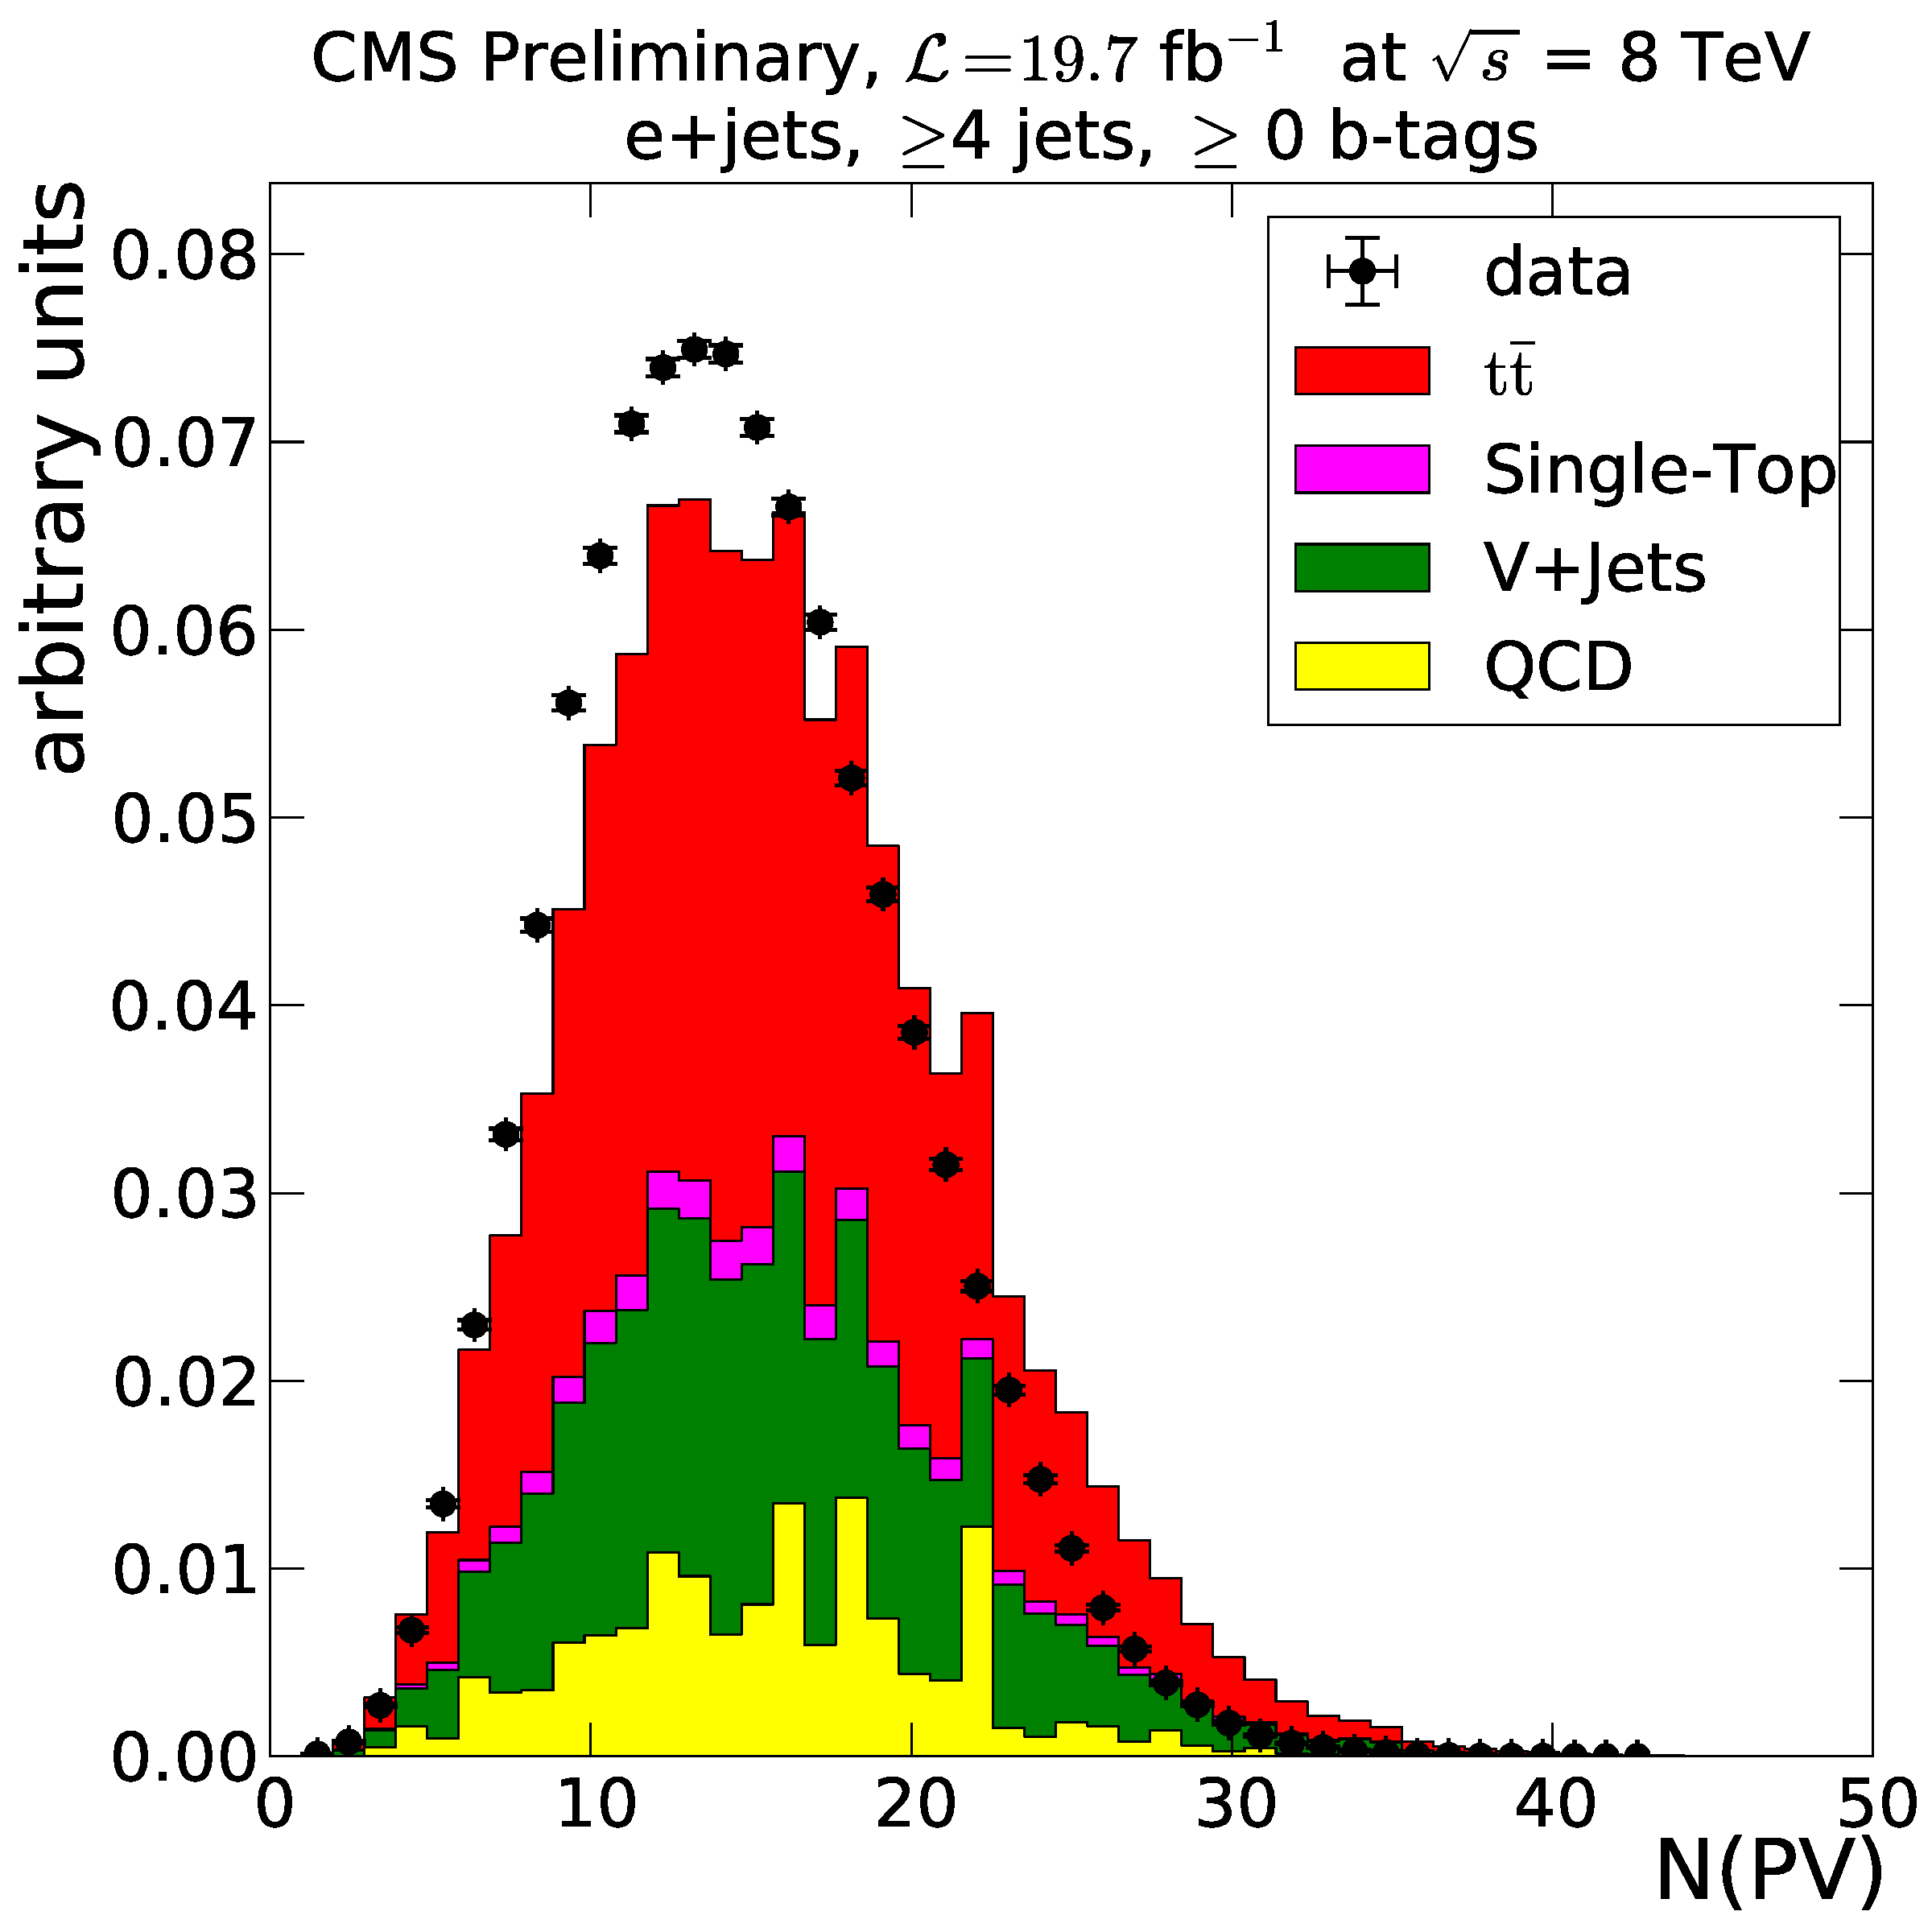
\includegraphics[width=0.50\textwidth]{vertices/EPlusJets_nVertex.pdf}}\hfill
	\subfloat[]{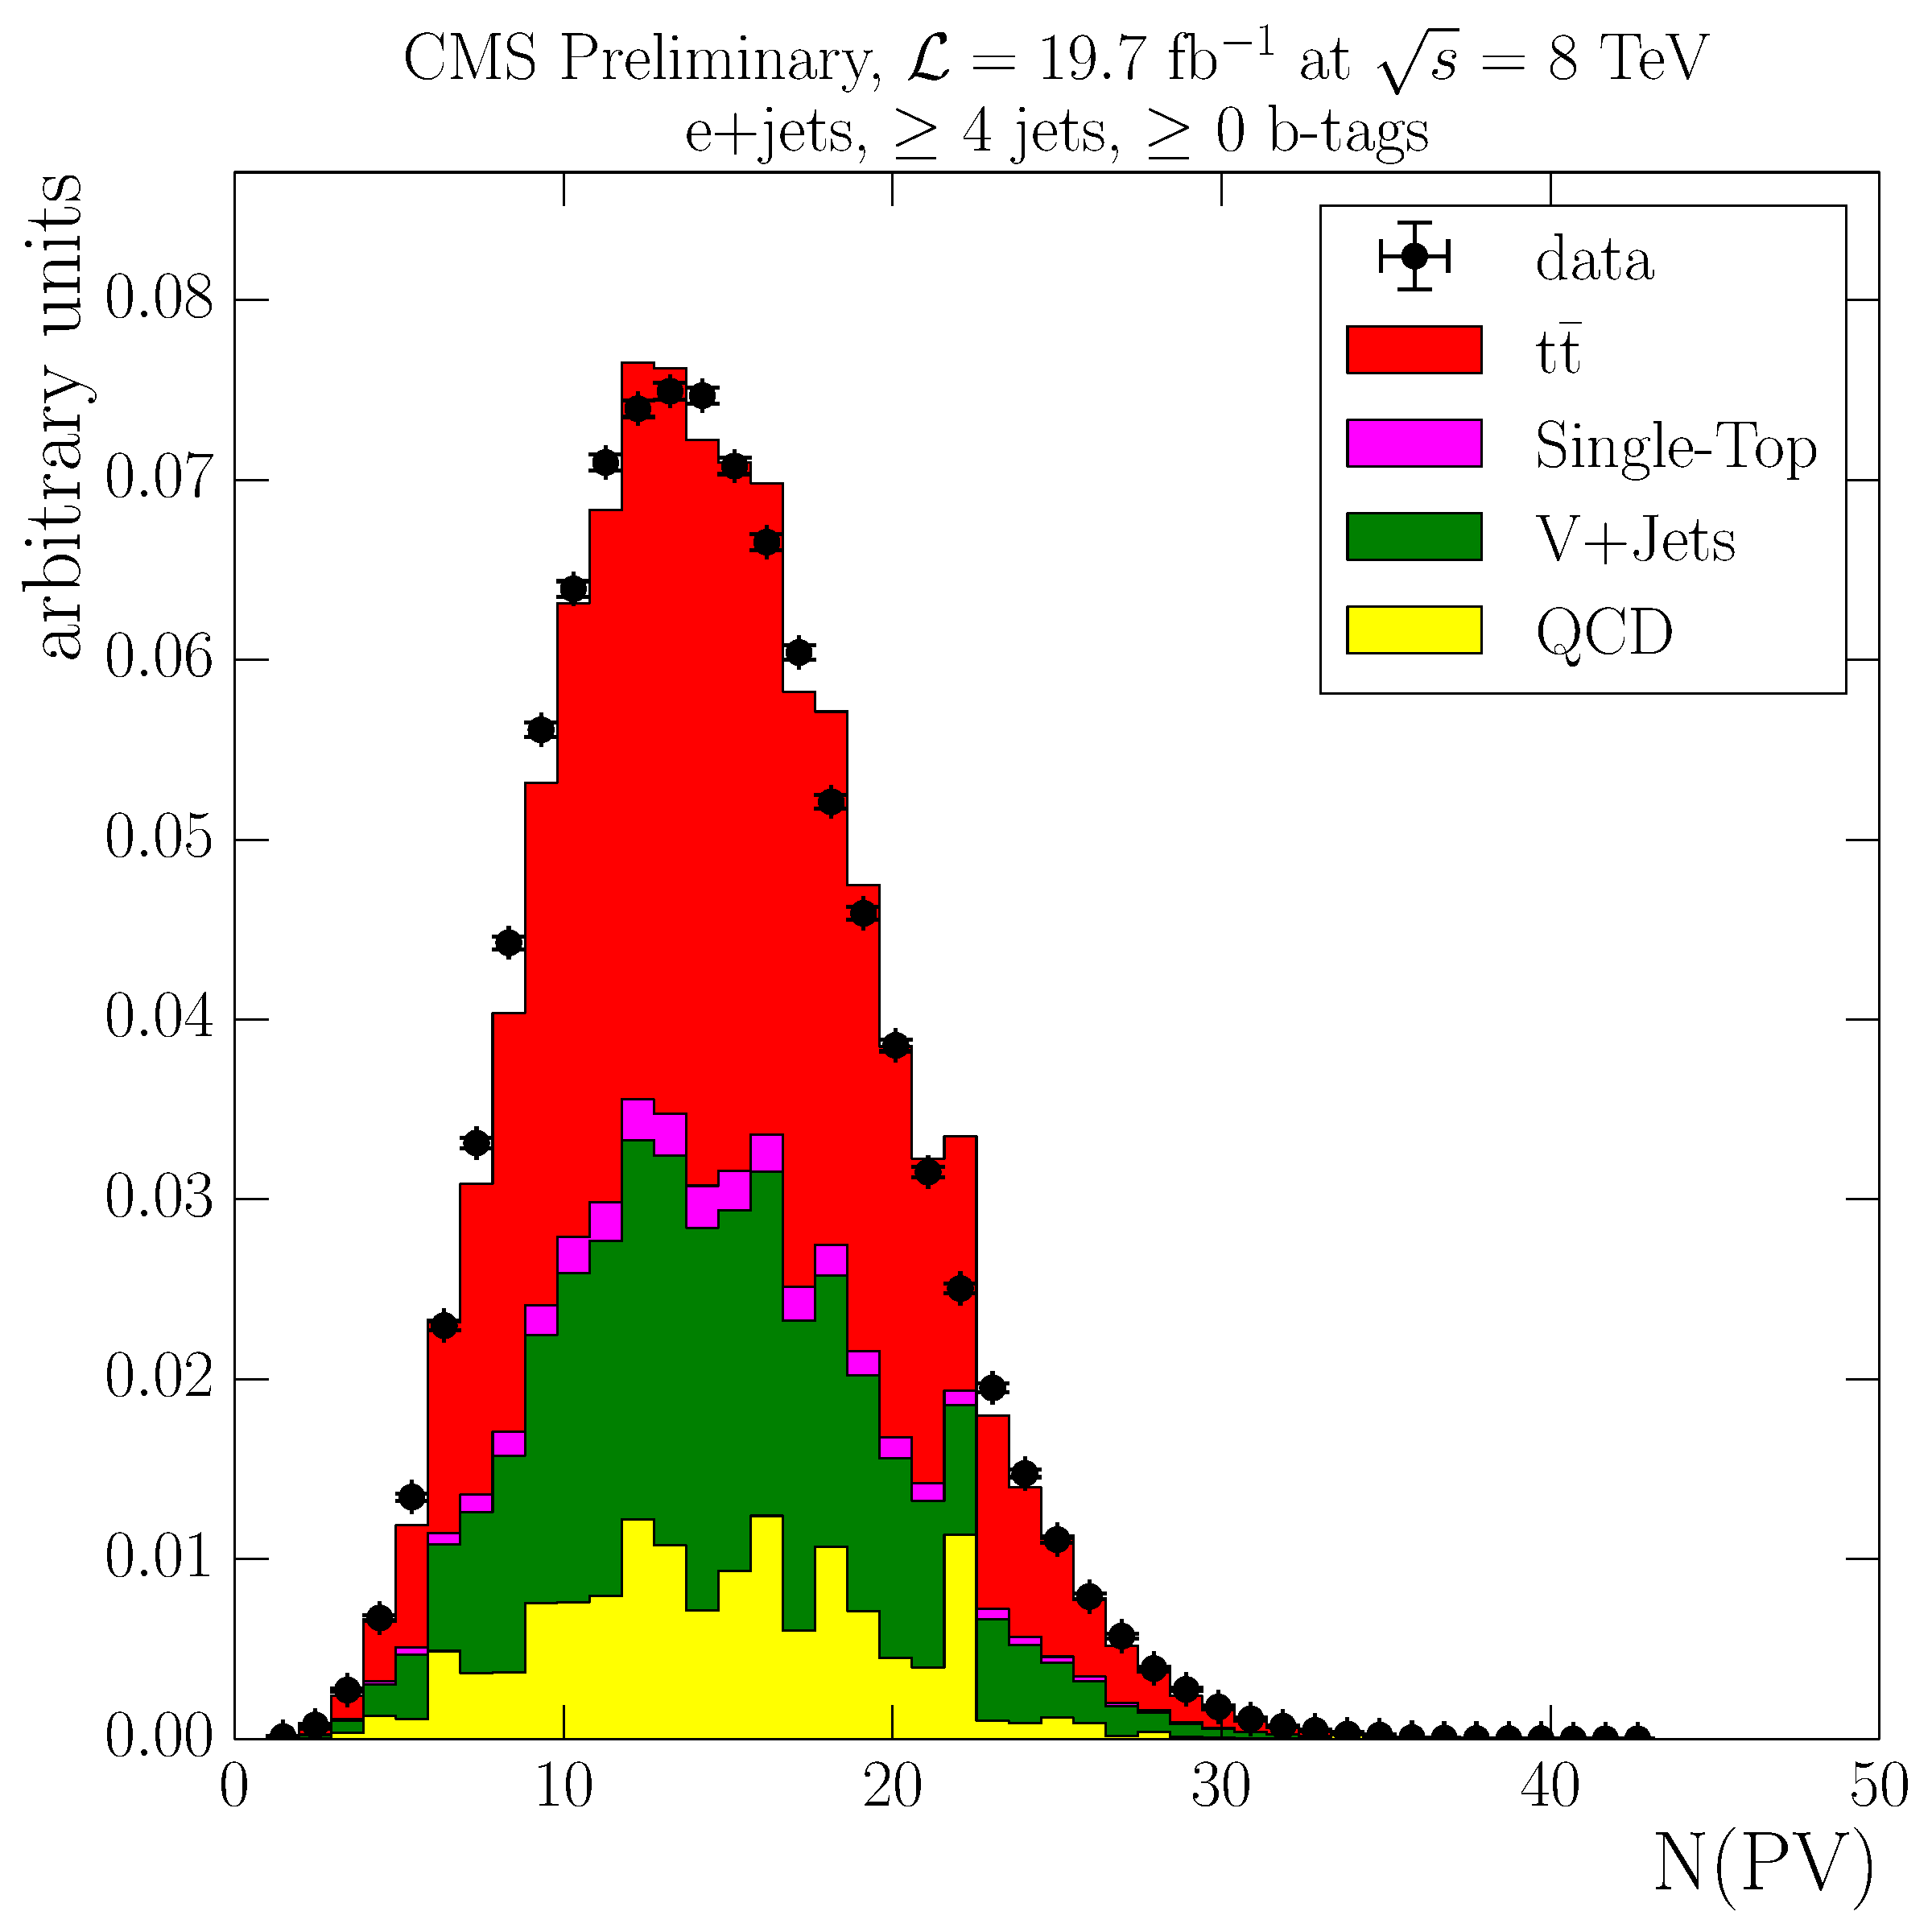
\includegraphics[width=0.50\textwidth]{vertices/EPlusJets_nVertex_reweighted.pdf}} \\
	\subfloat[]{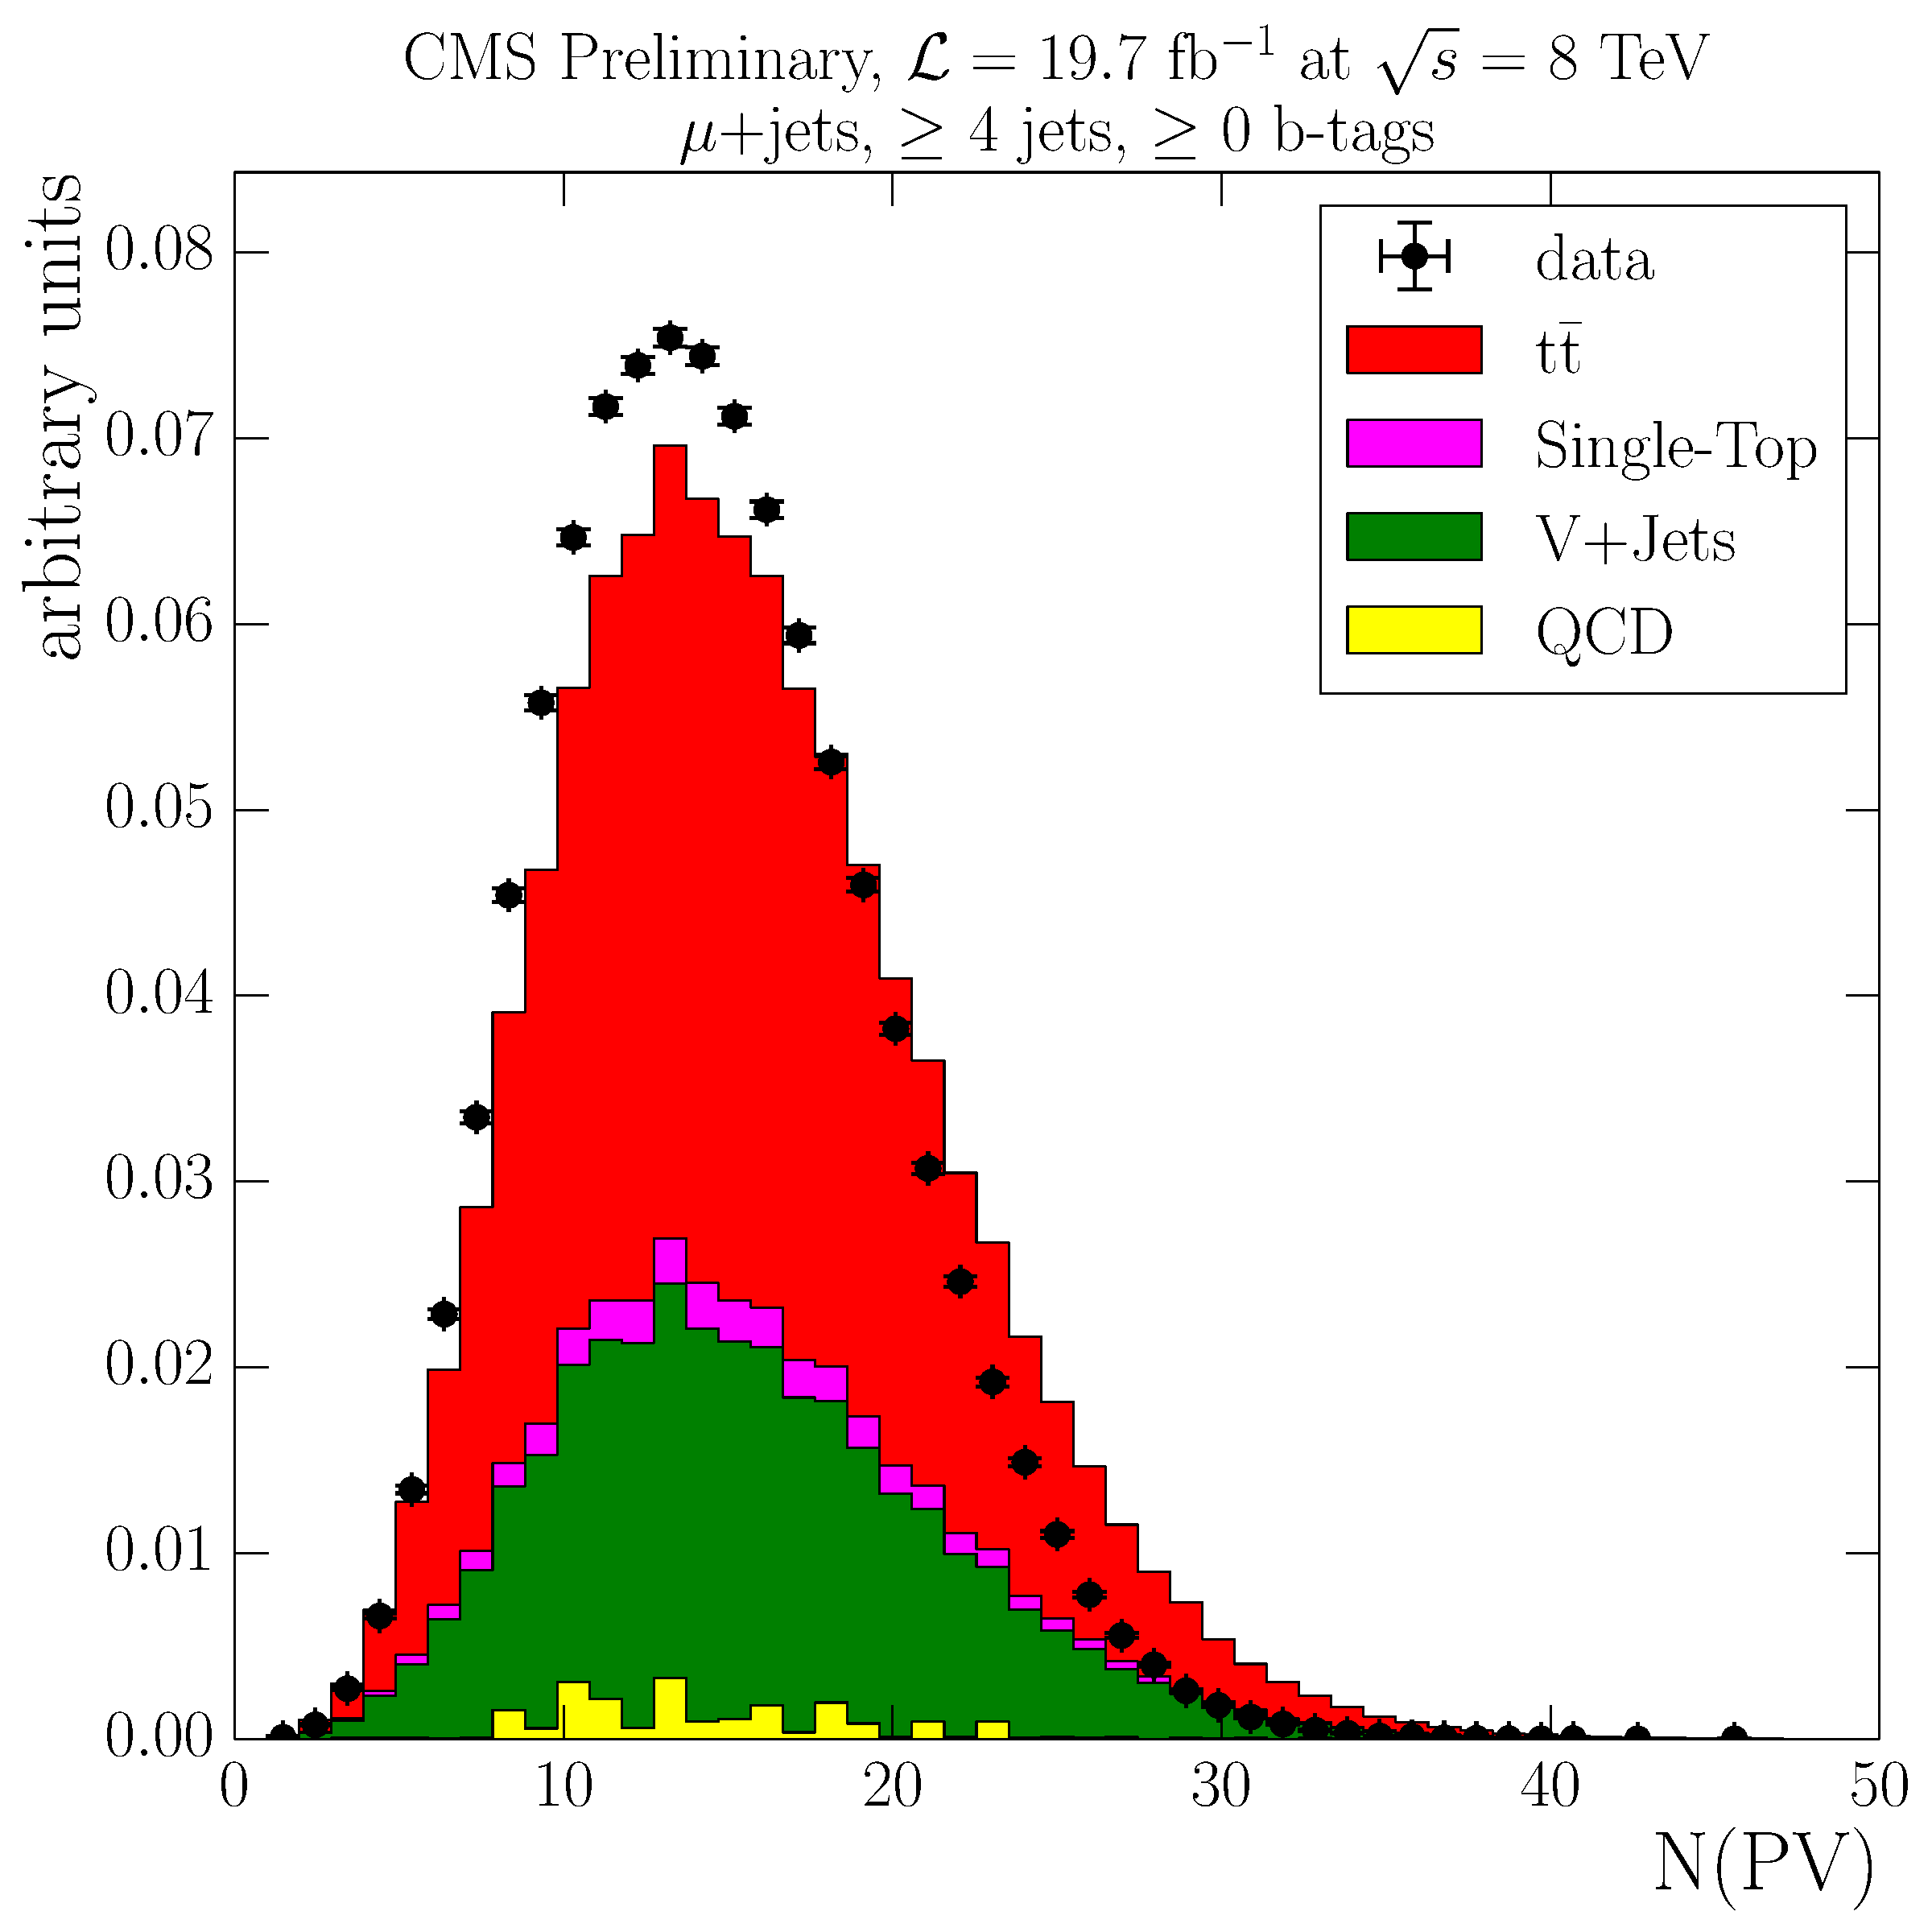
\includegraphics[width=0.50\textwidth]{vertices/MuPlusJets_nVertex.pdf}}\hfill
	\subfloat[]{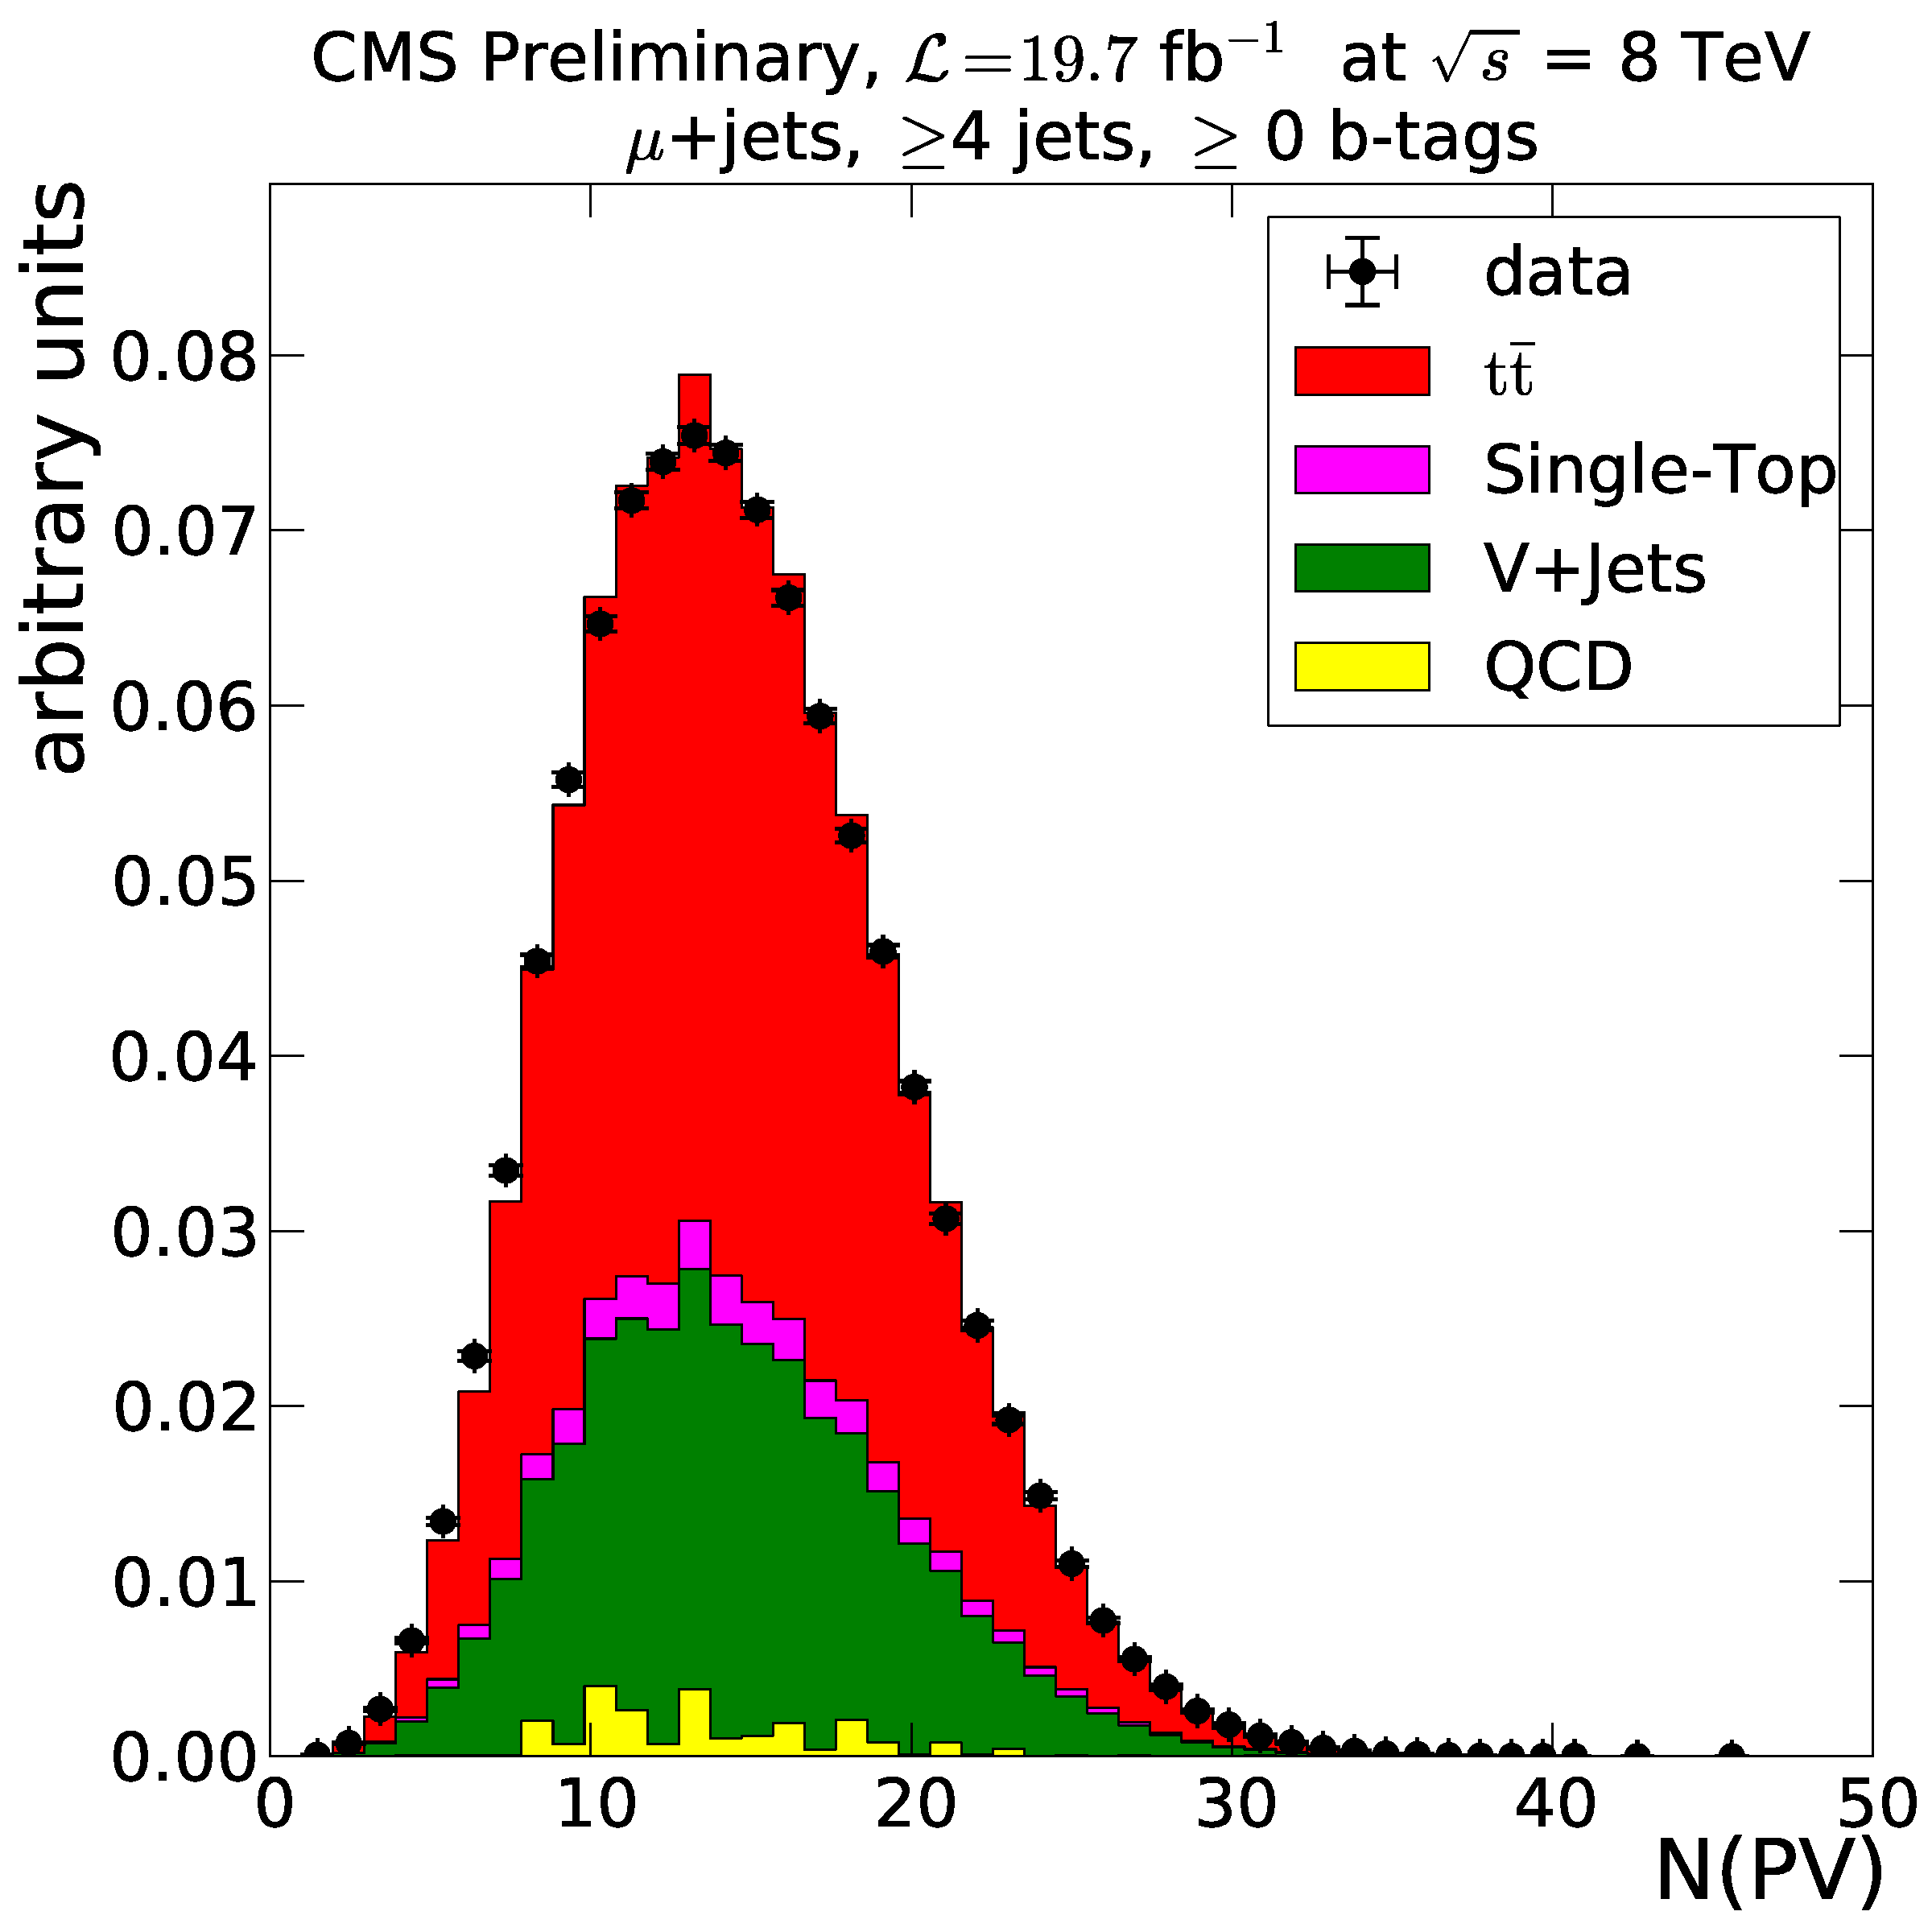
\includegraphics[width=0.50\textwidth]{vertices/MuPlusJets_nVertex_reweighted.pdf}}
    \caption[Number of reconstructed vertices per event before and after pile-up reweighting]{Number of reconstructed
    vertices per event before (left) and after pile-up reweighting (right) in the electron channel (top) and in the muon
    channel (bottom). Both data and sum of the MC samples are normalised to unit area.}
    \label{fig:pileup_vertices}
    %QCD is estimated from MC here. Possible to fix/remove?
\end{figure}

To estimate the number of pile-up vertices in data, the measured instantaneous luminosity in each bunch crossing is
multiplied by an average total inelastic proton-proton cross section. Therefore, two sources of uncertainty arise from
these factors: the luminosity uncertainty, measured to be \SI{4.4}{\pc} by a dedicated study \autocite{CMS_lumi_2012},
and the uncertainty on the total inelastic cross section. To obtain the total cross section value, the CMS measurement
of \SI{68\pm4.5}{\milli\barn} based on \SI{7}{\TeV} data \autocite{CMS_total_inelastic_7TeV} was extrapolated to the
\SI{8}{\TeV} value of \SI{69.3}{\milli\barn}. The recommended uncertainty on this value, set to be \SI{5}{\pc}, covers
the modelling and physics aspects of pile-up simulation that have not been fully studied up to date.

%https://twiki.cern.ch/twiki/bin/viewauth/CMS/PileupSystematicErrors (this has been updated to 69.4mb!)

The effect of the \SI{\pm5}{\pc} variations in total inelastic cross section on the estimate of the true number of
vertices in data is shown in Figure~\ref{fig:pileup_truth}, whereas its effect on the simulated distributions is shown
in Figure~\ref{fig:pileup_vertices_variations} for both electron and muon channels.

 \begin{figure}[htbp]
   	\centering
    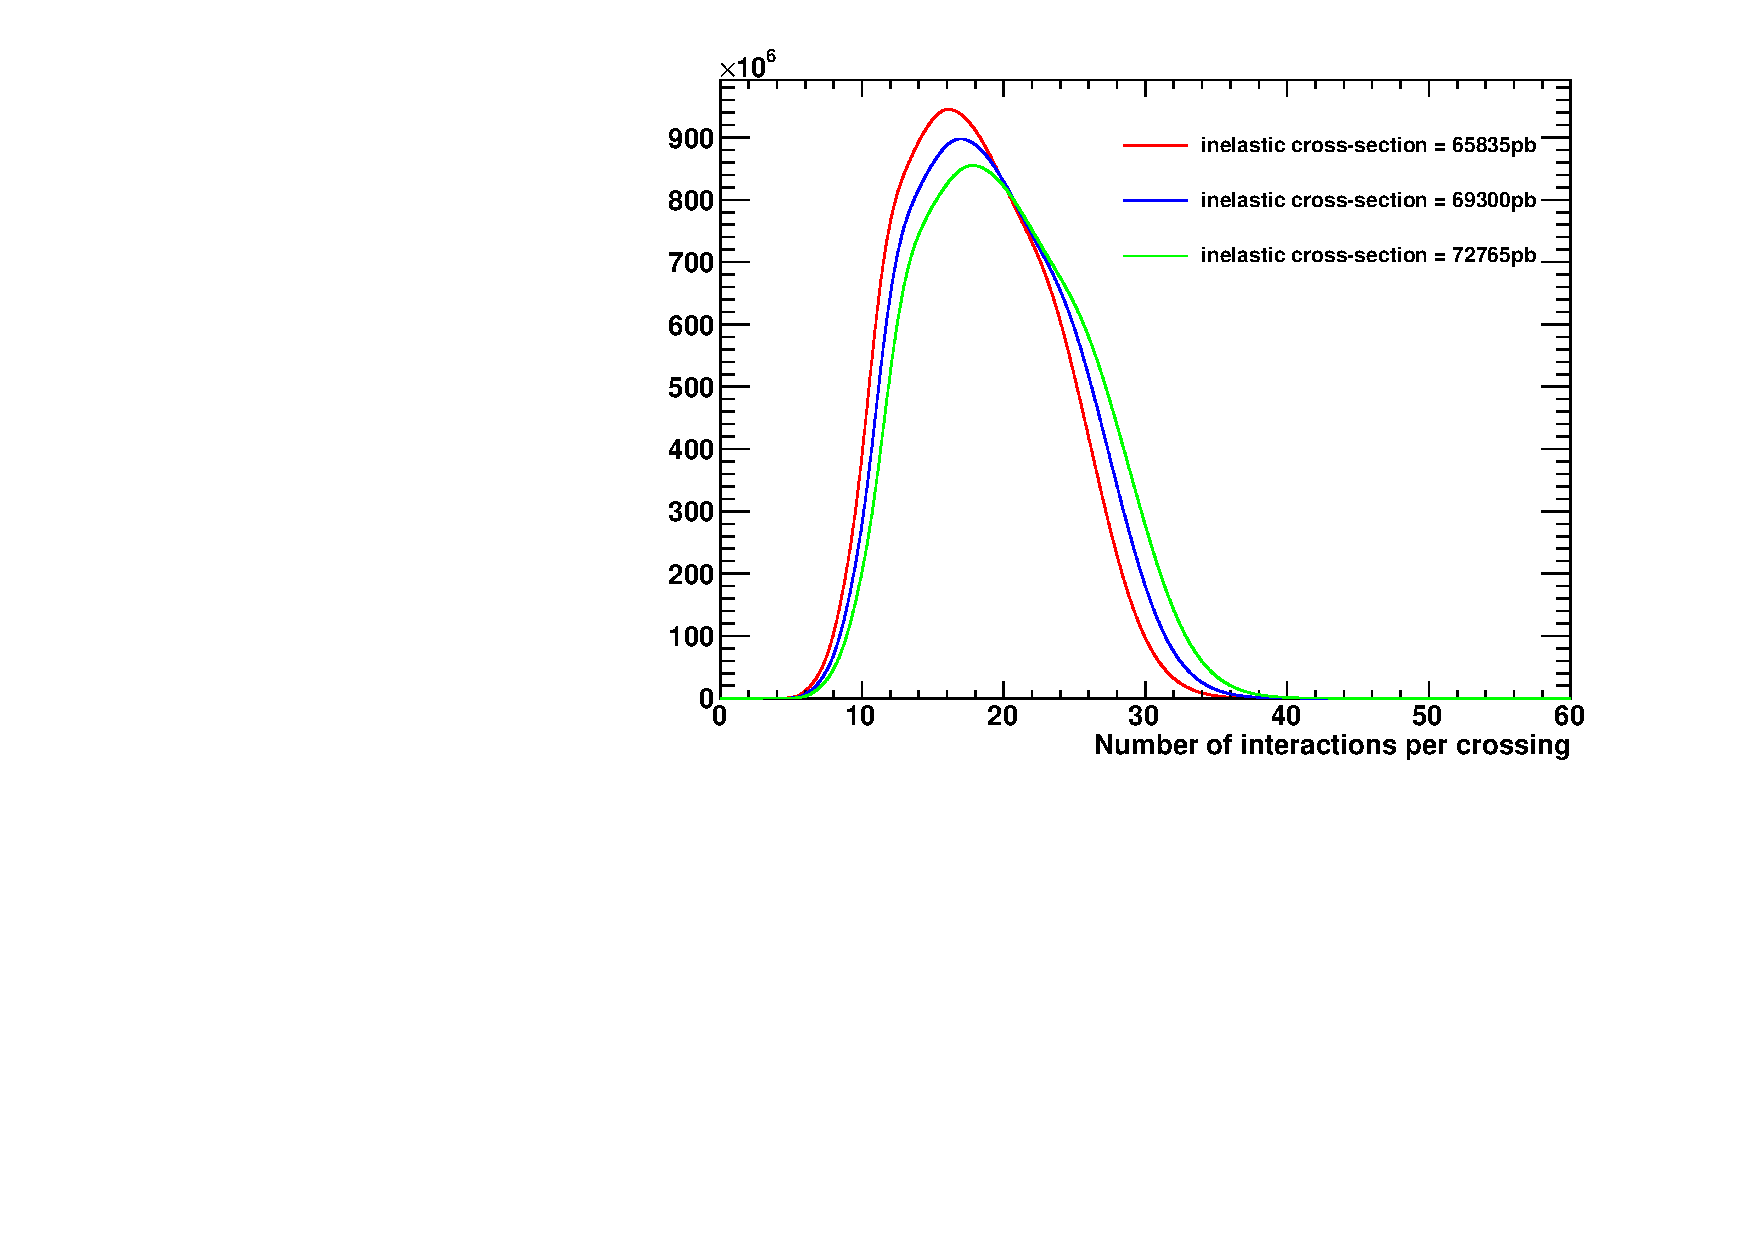
\includegraphics[width=\textwidth]{vertices/PileUp_2012_truth_data.pdf}
    \caption[Number of expected vertices per event for central and $\pm1\sigma$ variations of the total inelastic cross
    section for the 2012 data]{Number of expected vertices per event for central and $\pm1\sigma$ variations of the
    total inelastic cross section for the 2012 data.}
    \label{fig:pileup_truth}
 \end{figure}

\begin{figure}[!htpb]
	\centering
	\subfloat[]{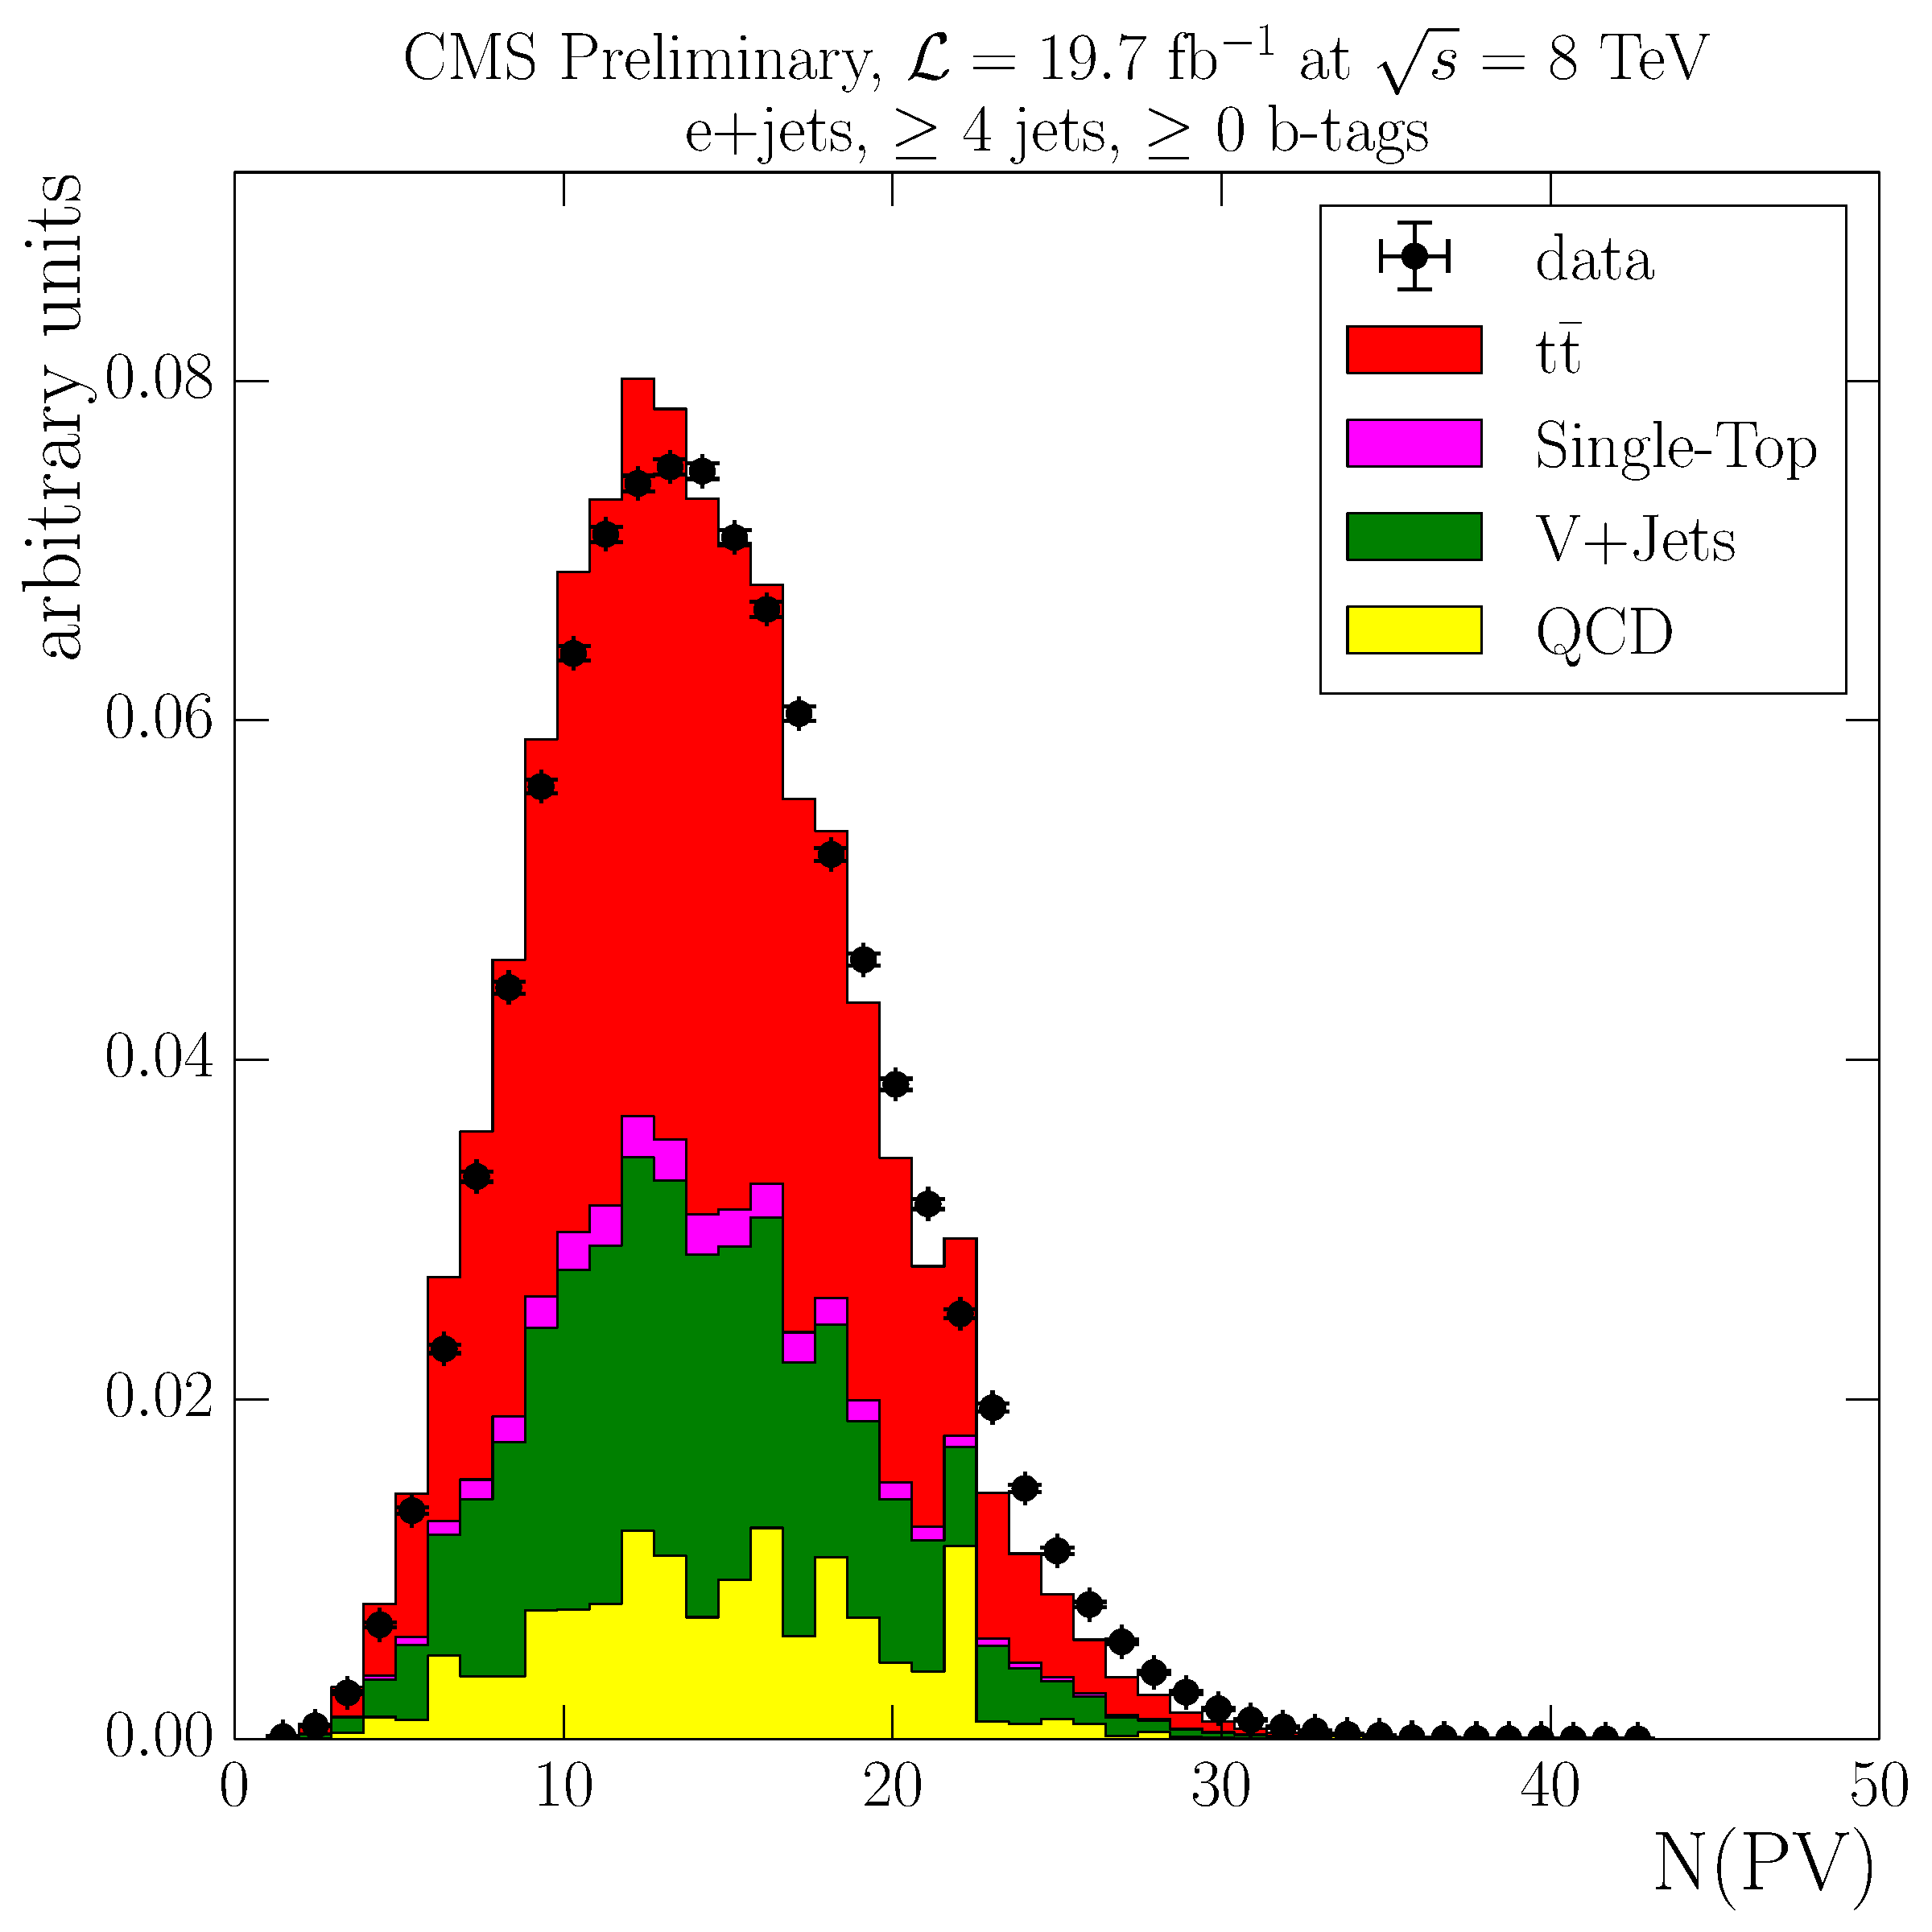
\includegraphics[width=0.50\textwidth]{vertices/EPlusJets_nVertex_reweighted_PU_down.pdf}}\hfill
	\subfloat[]{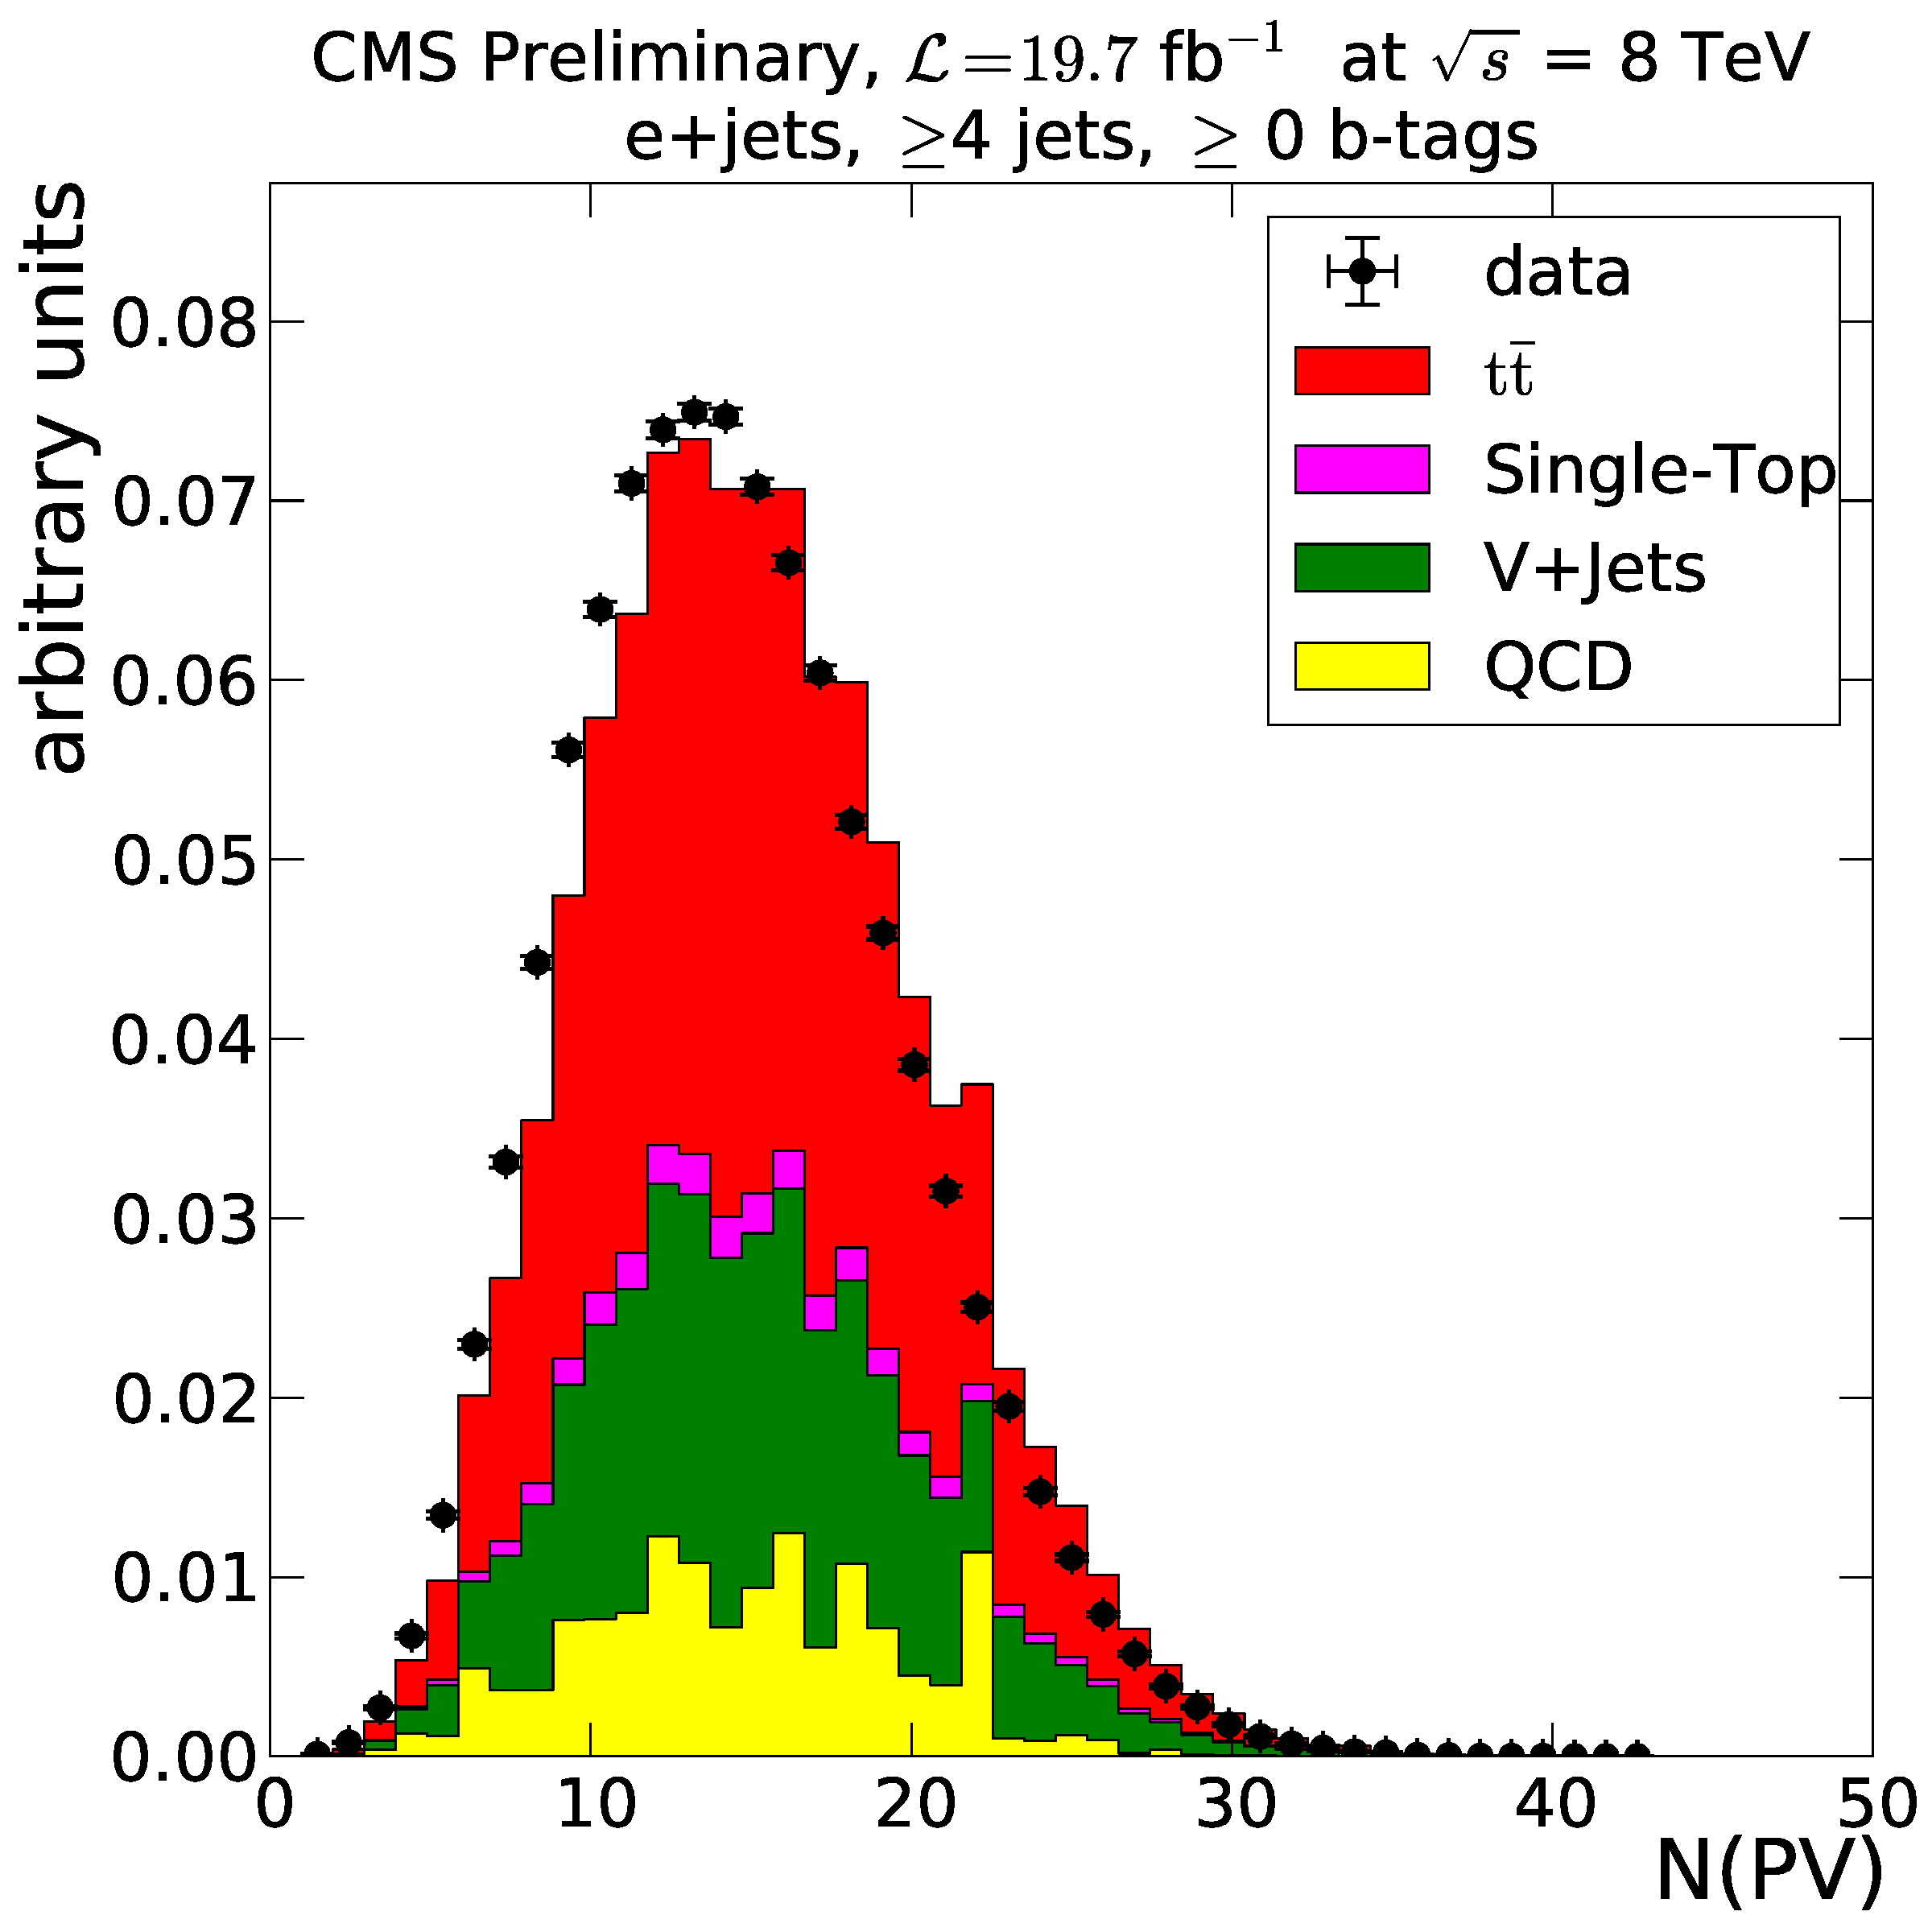
\includegraphics[width=0.50\textwidth]{vertices/EPlusJets_nVertex_reweighted_PU_up.pdf}} \\
	\subfloat[]{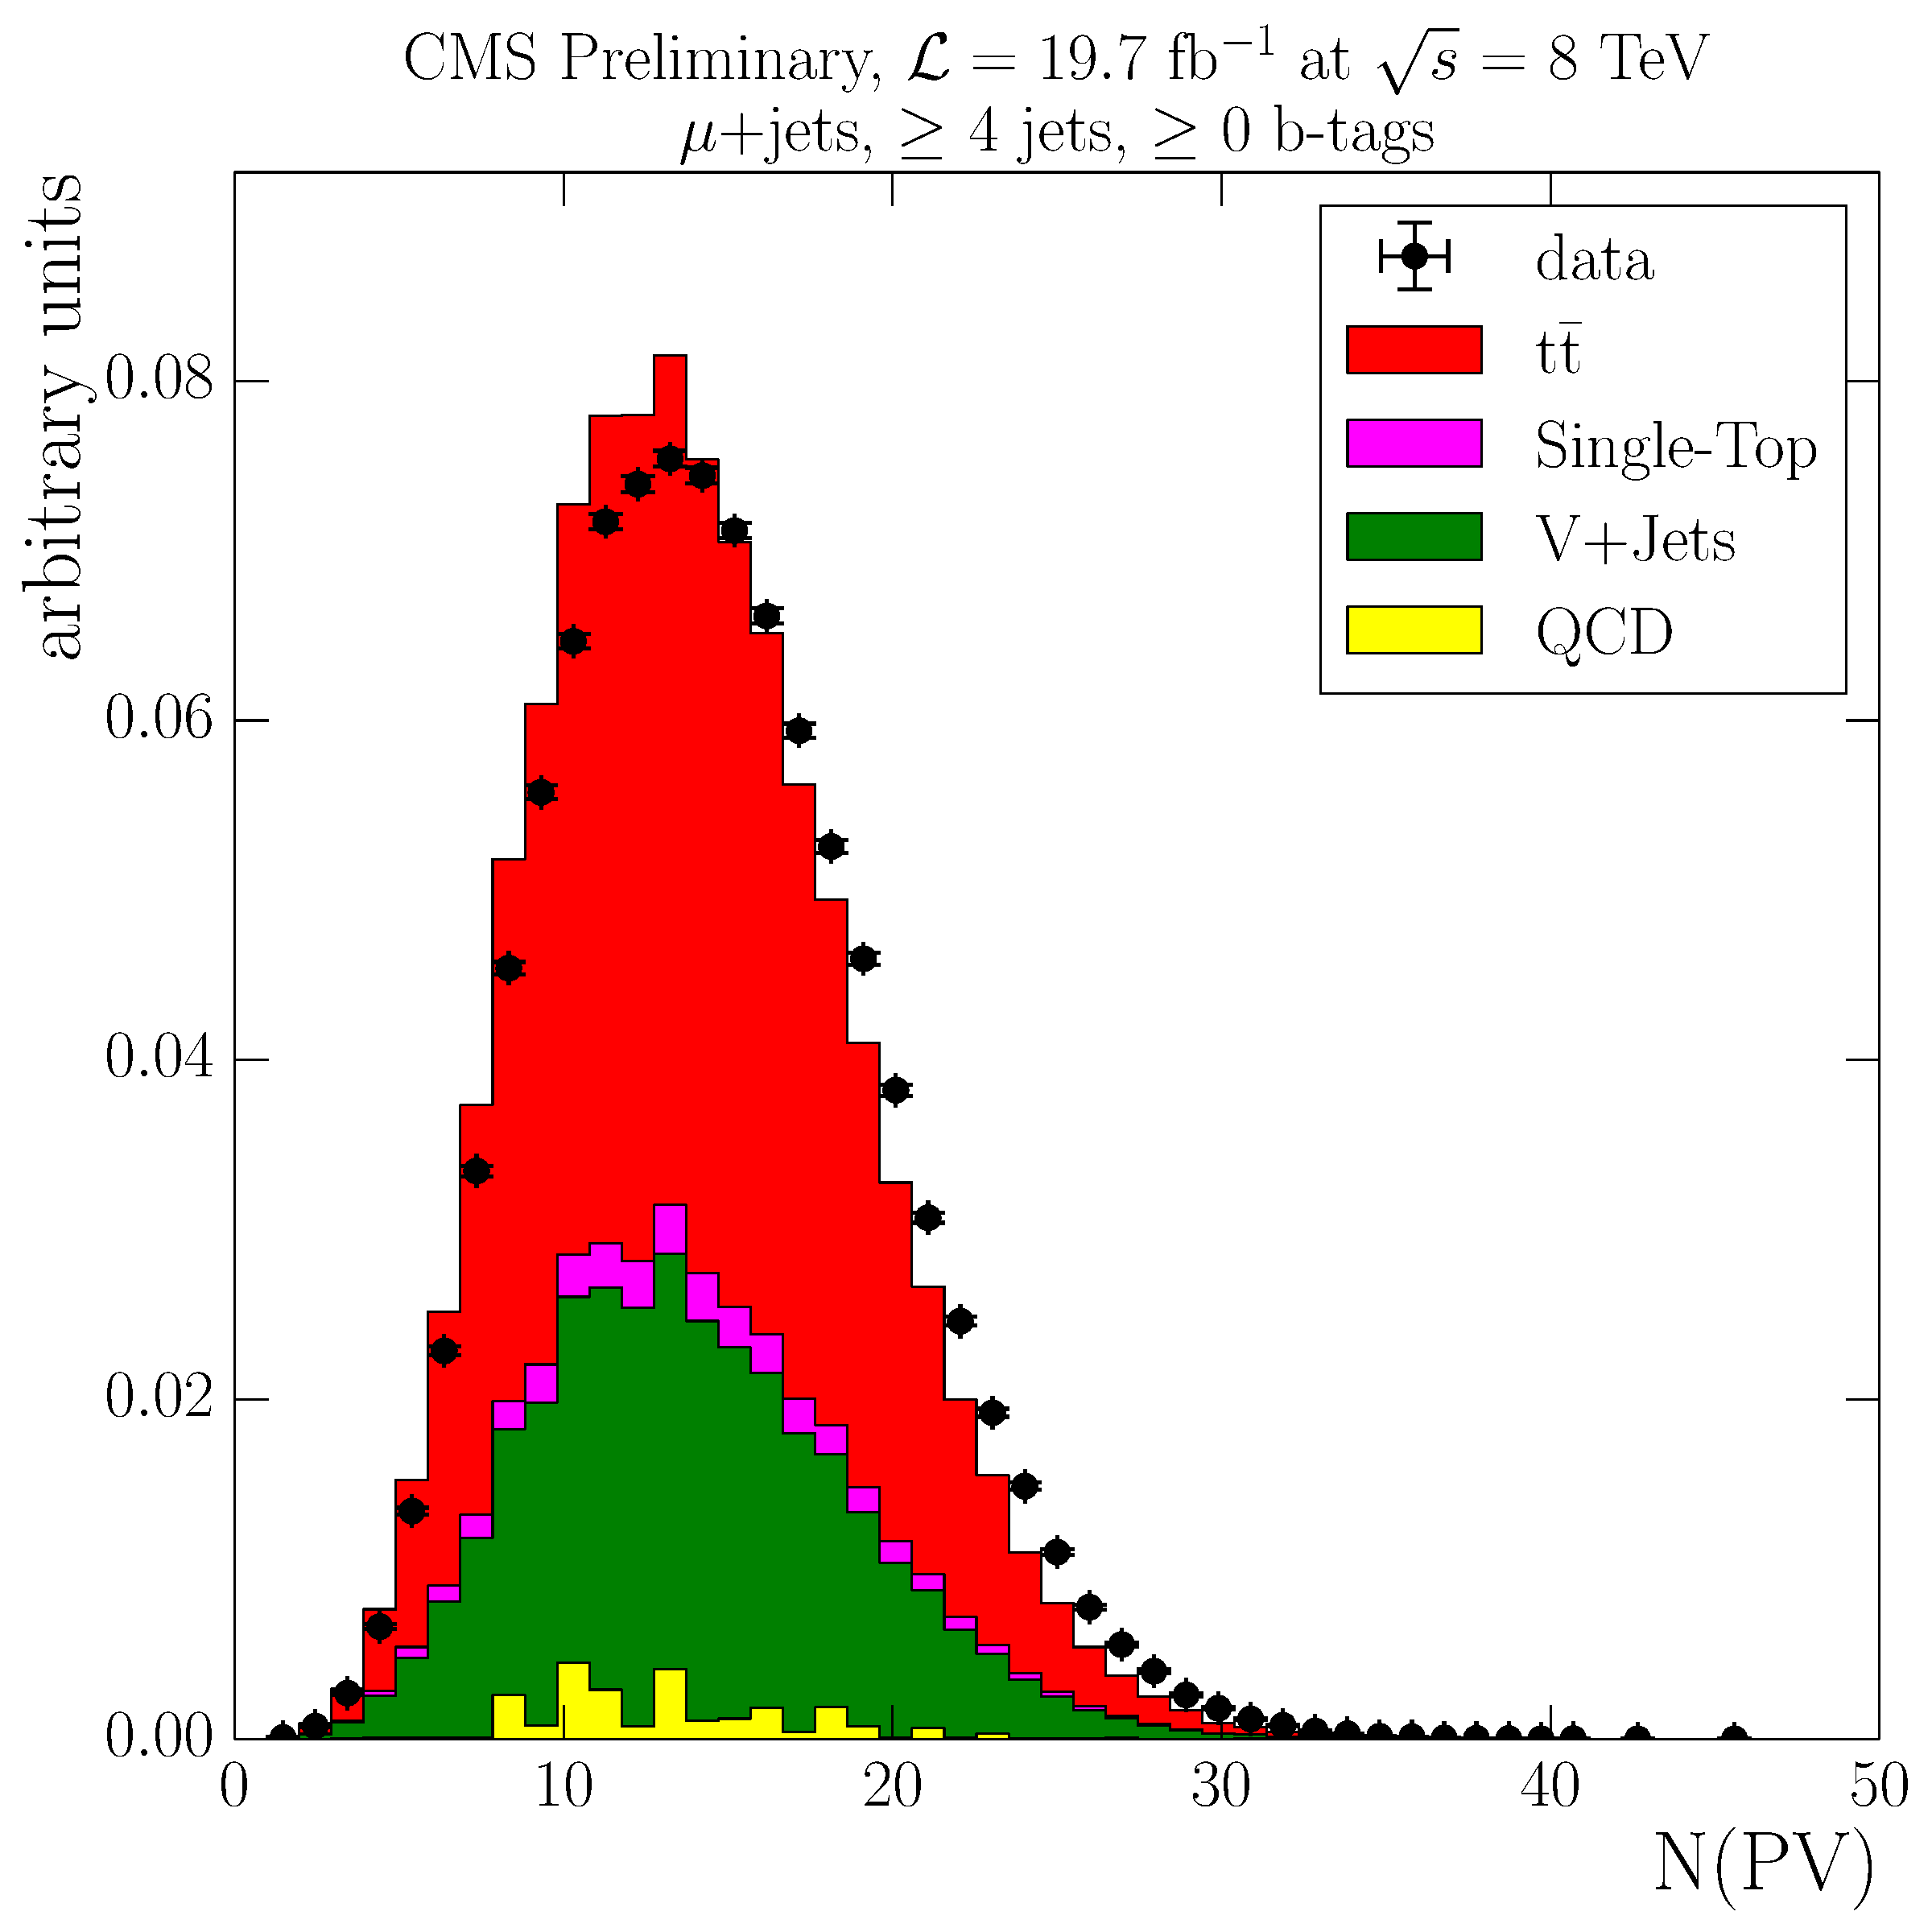
\includegraphics[width=0.50\textwidth]{vertices/MuPlusJets_nVertex_reweighted_PU_down.pdf}}\hfill
	\subfloat[]{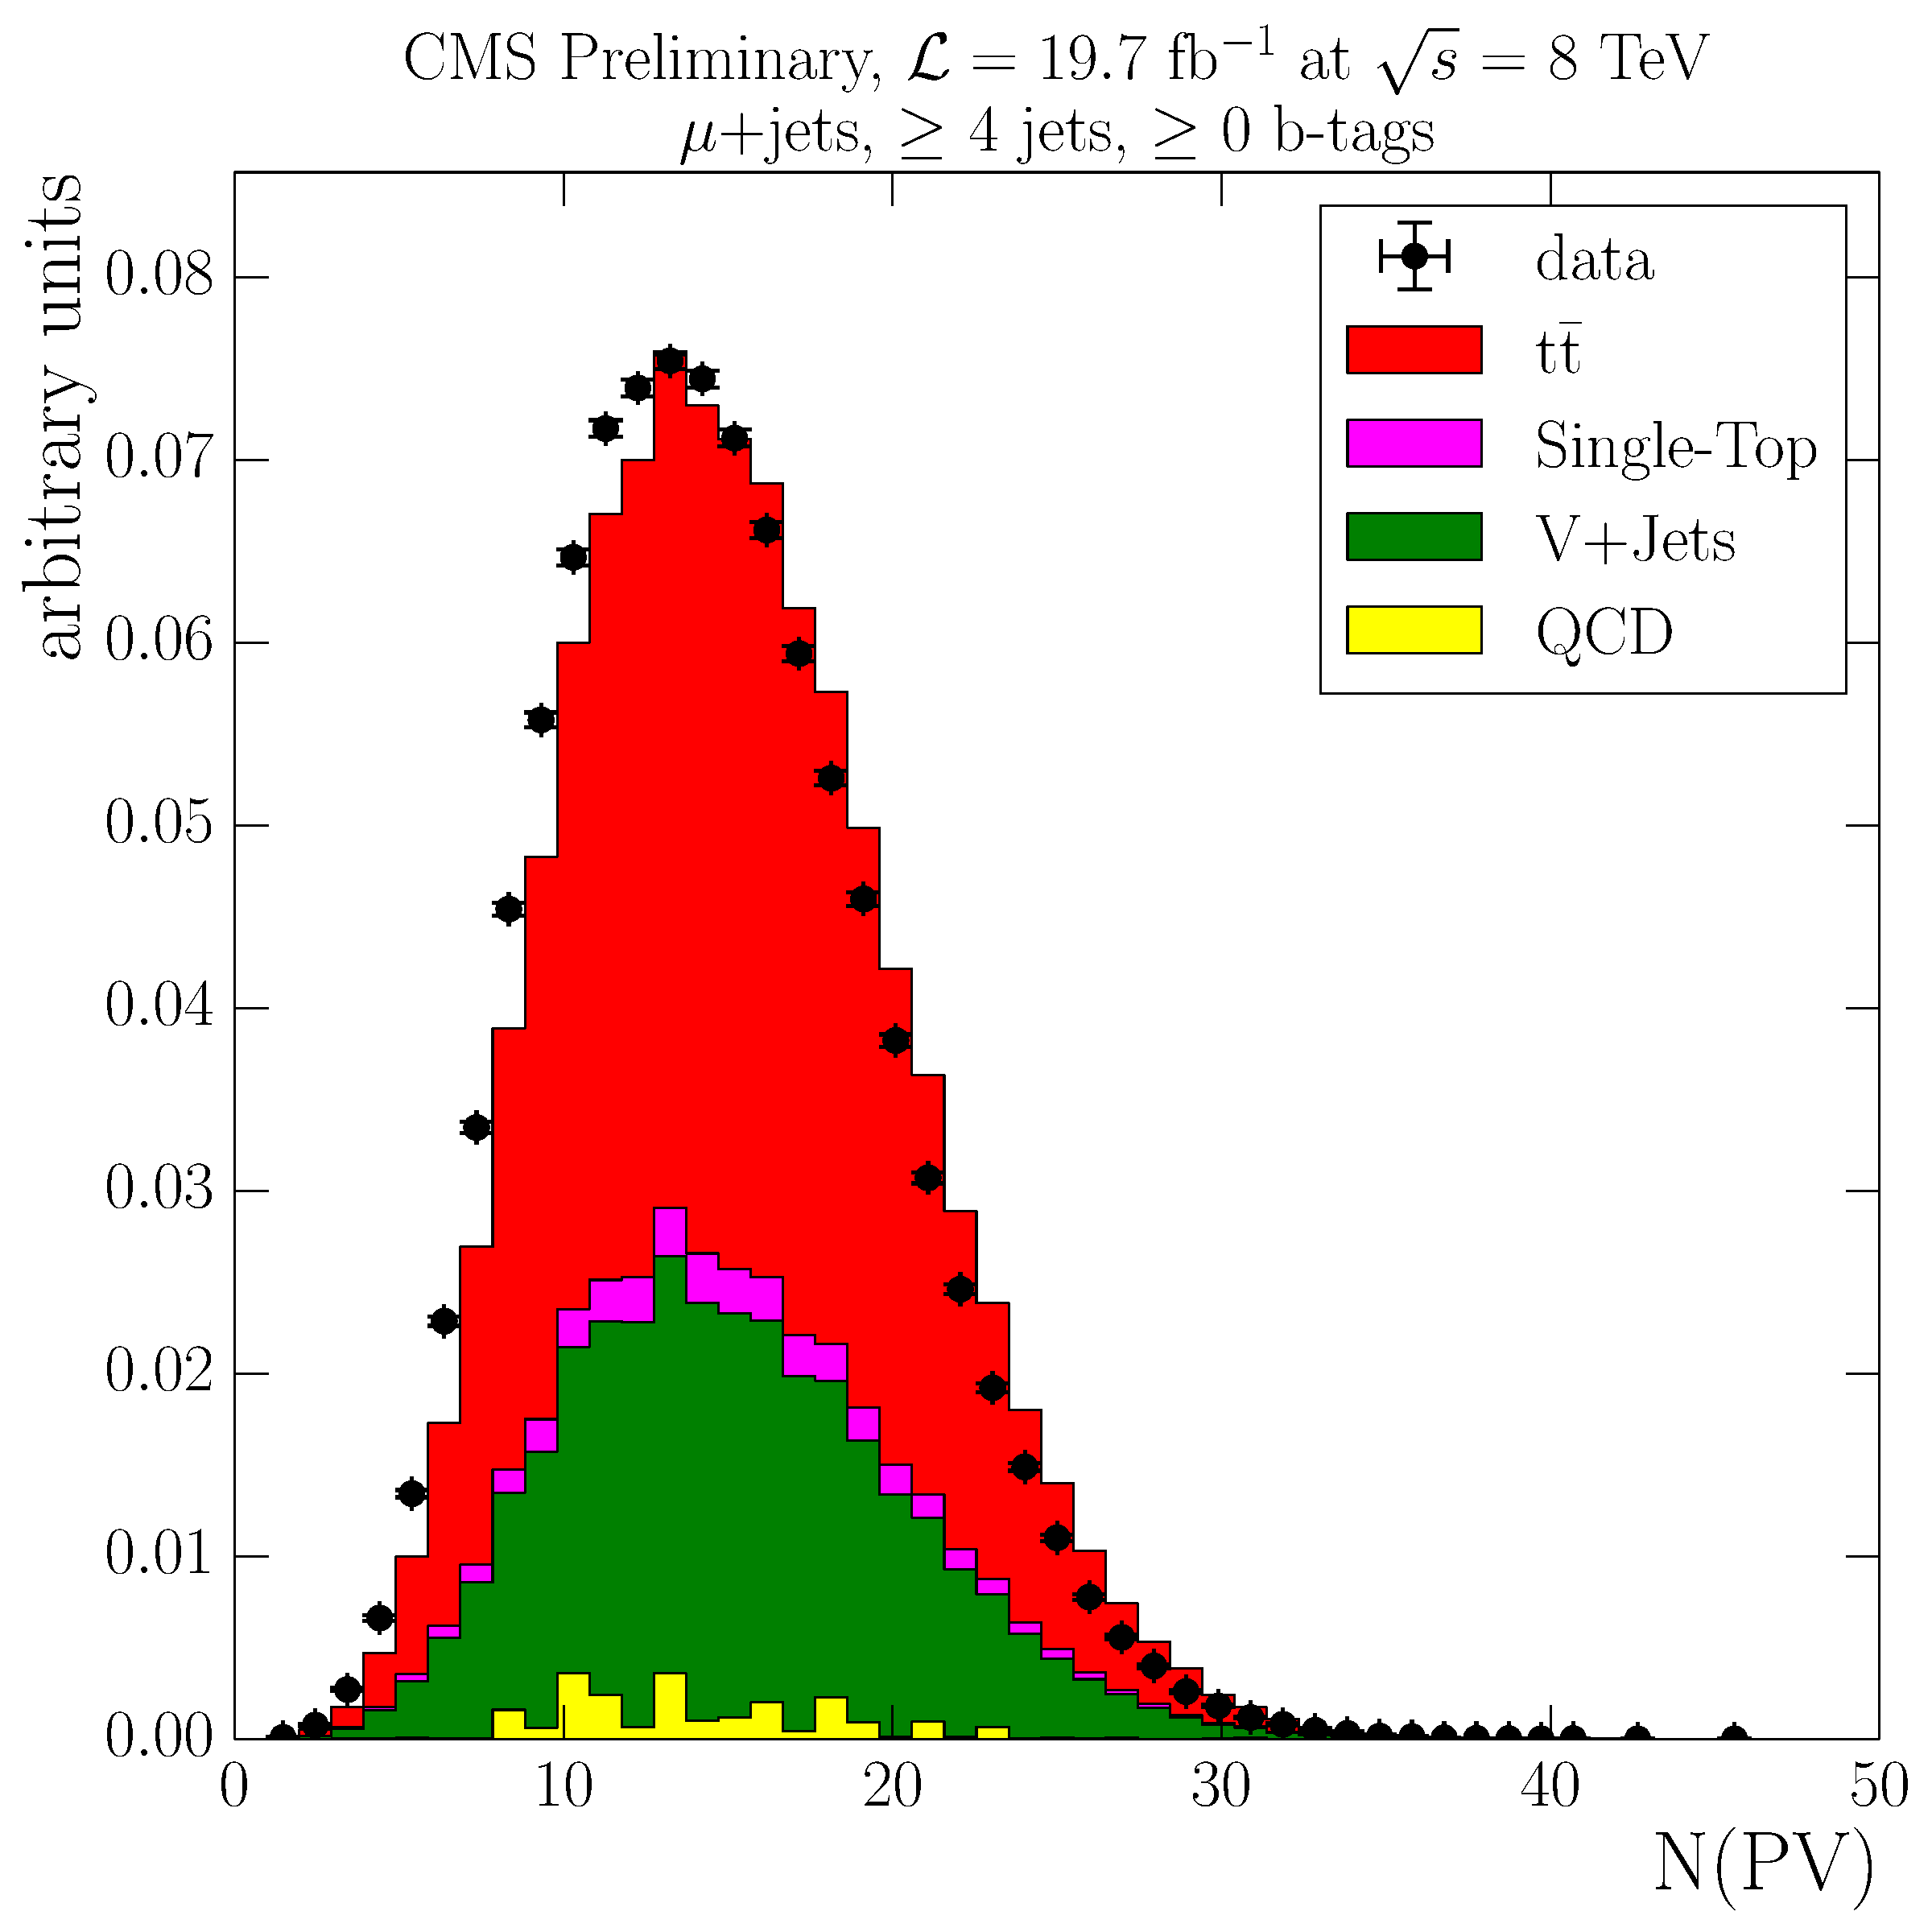
\includegraphics[width=0.50\textwidth]{vertices/MuPlusJets_nVertex_reweighted_PU_up.pdf}}
    \caption[Number of reconstructed vertices per event for $\pm1\sigma$ variations of the pile-up reweighting
    procedure]{Number of reconstructed vertices per event for $-1\sigma$ (left) and $+1\sigma$ variation (right) of the
    pile-up reweighting procedure for the electron channel (top) and the muon channel (bottom).}
    \label{fig:pileup_vertices_variations}
\end{figure}


\subsection{b-tagging corrections}
\label{ss_xsection:btagging_corrections}
In order to mitigate the background (QCD in particular), b-tagging is applied in the event selection of this analysis.
Similarly to the top quark mass analysis, the CSV algorithm with the medium working point providing
\SI{\sim70}{\percent} efficiency and \SI{\sim1}{\percent} mis-tag rate (Section~\ref{sss:b-tagging}) was used. However,
in contrast with the 2011 analysis where the b-tagging corrections were implemented in the construction of the event
likelihood, in this work scale factors are applied to Monte Carlo events. This is done in order to correct for the
mismatch between the algorithm efficiency seen in data and MC \autocite{btagging_CMS_8TeV_results}. \pt and
$\eta$-dependent scale factors were derived by the CMS b-tag Physics Object Group \autocite{btag_weights_2011} and are
used to reweight the simulated events. The overall jet content of the event is taken into account, such as the number of
jets originating from light and heavy quarks.

\begin{figure}[!htpb]
	\centering
	\subfloat[]{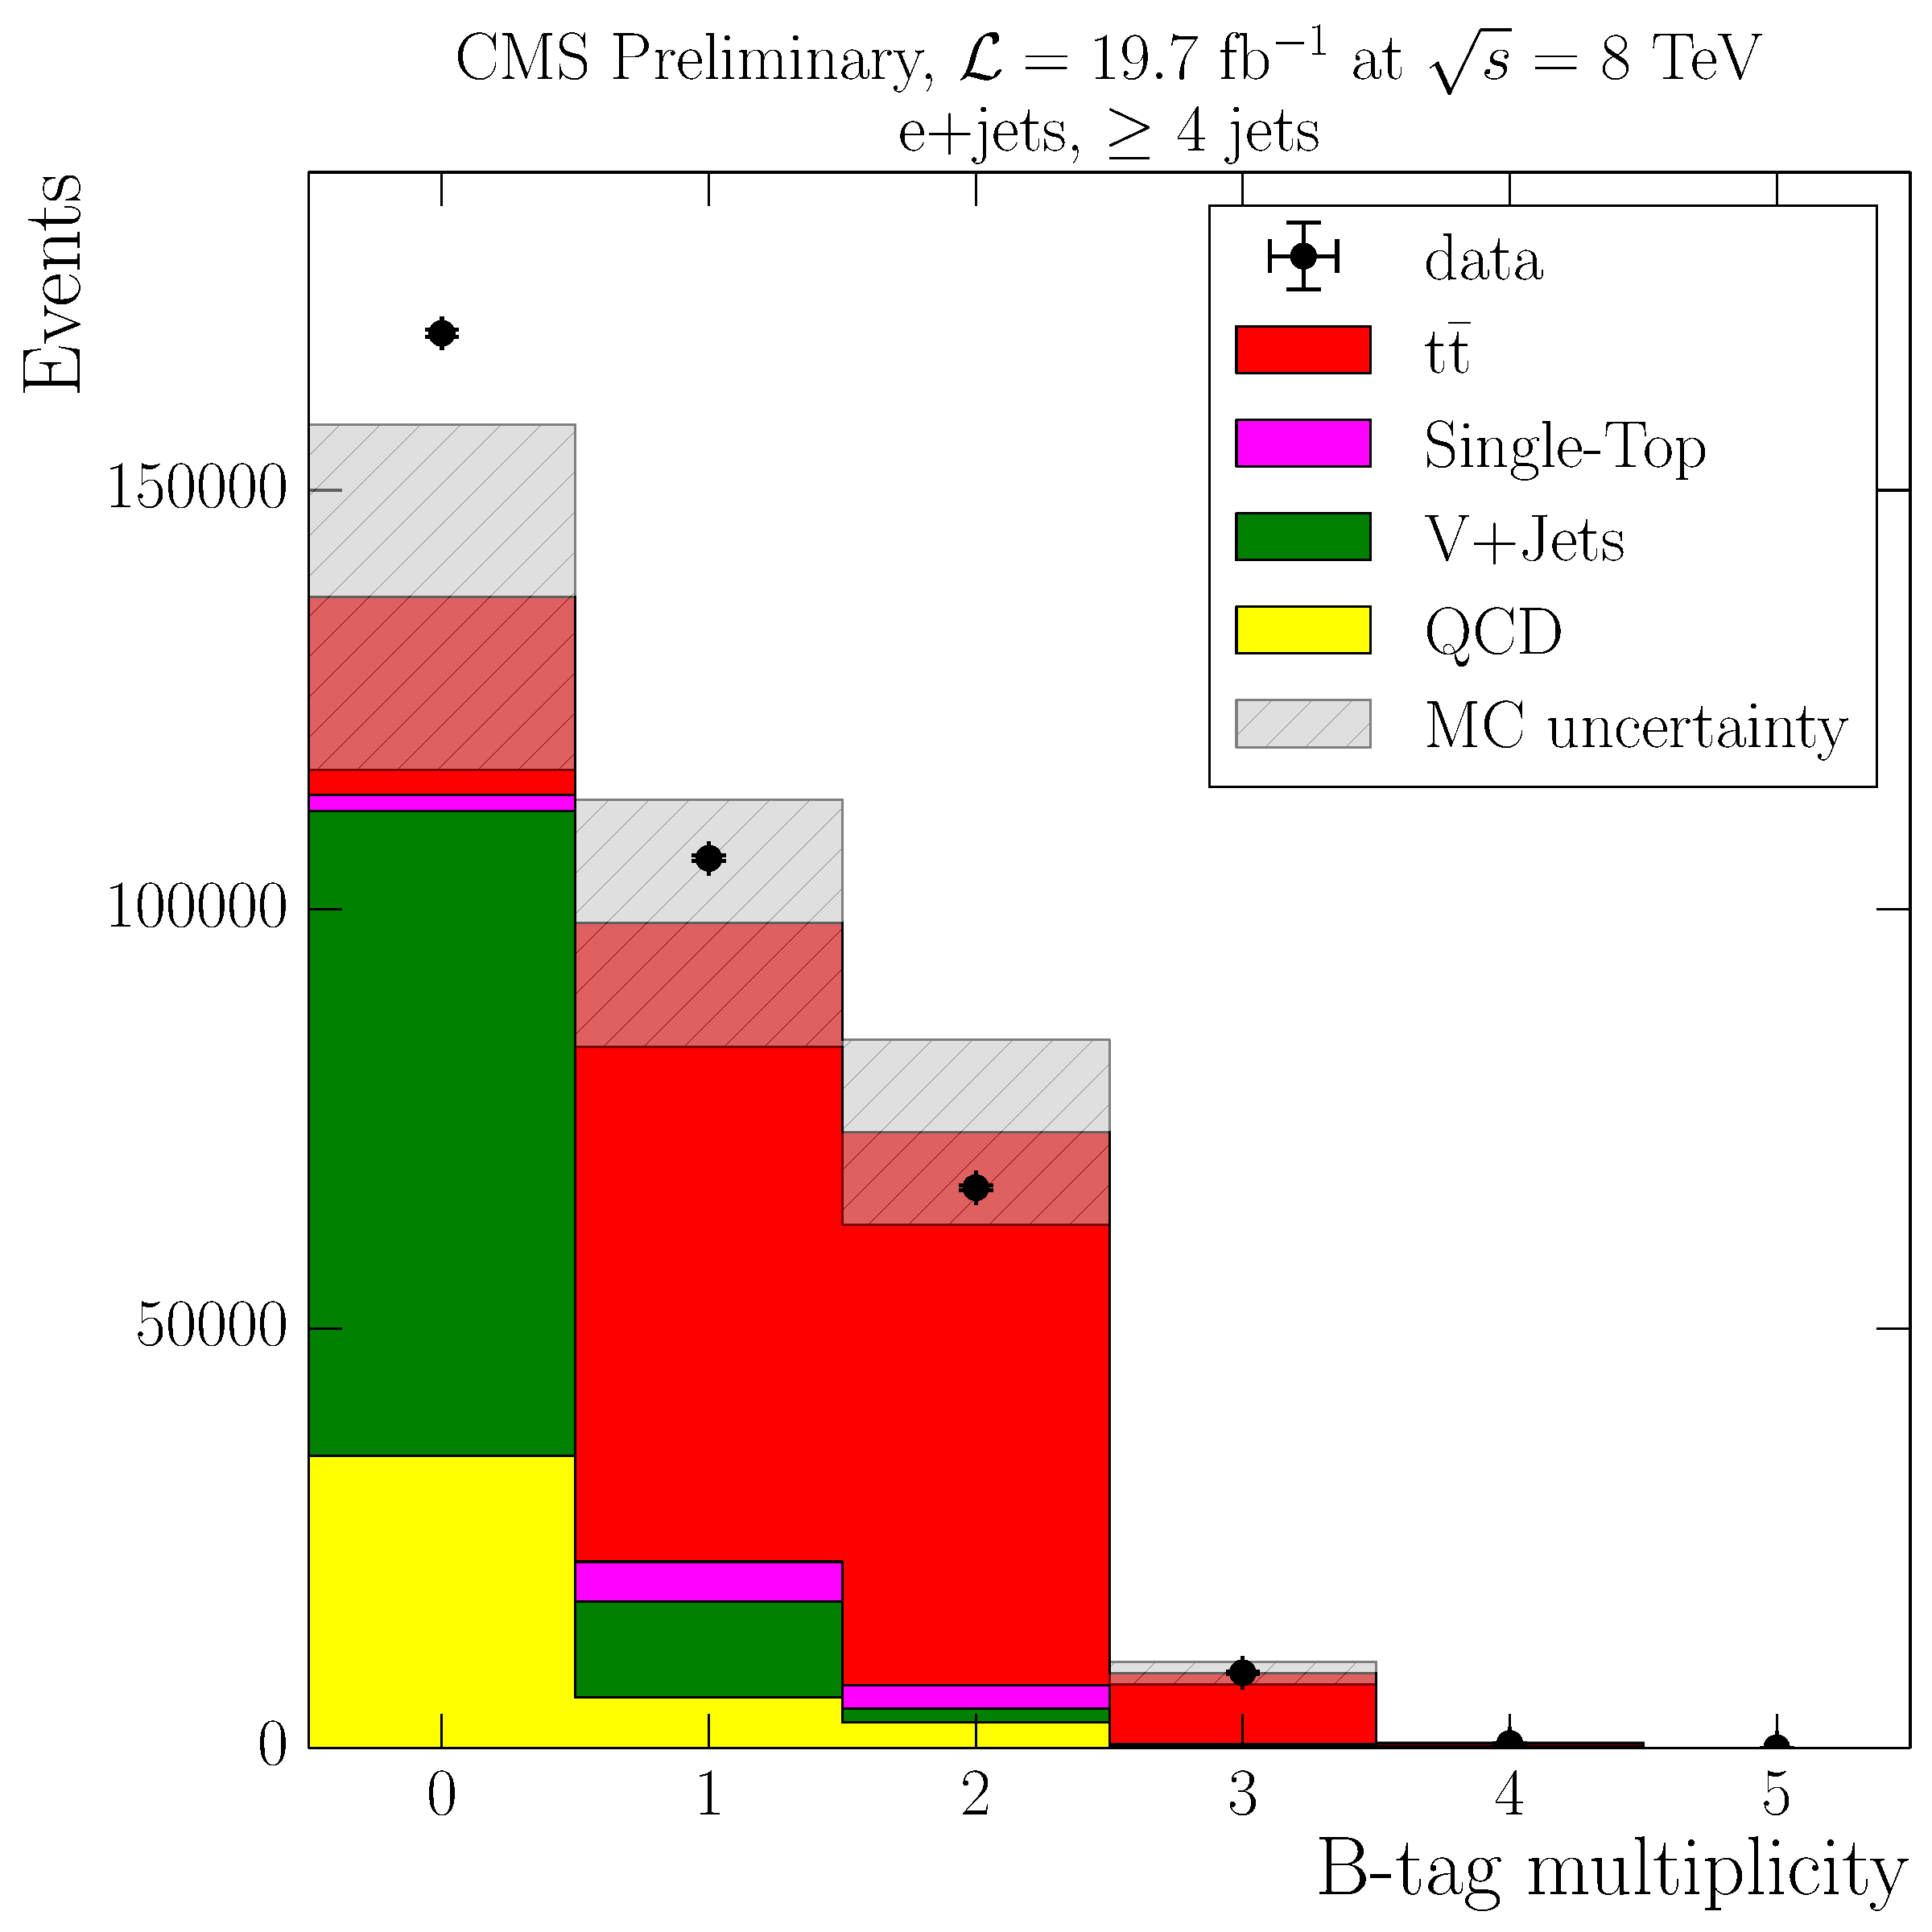
\includegraphics[width=0.50\textwidth]{bjets_multiplicity/EPlusJets_N_BJets.pdf}}\hfill
	\subfloat[]{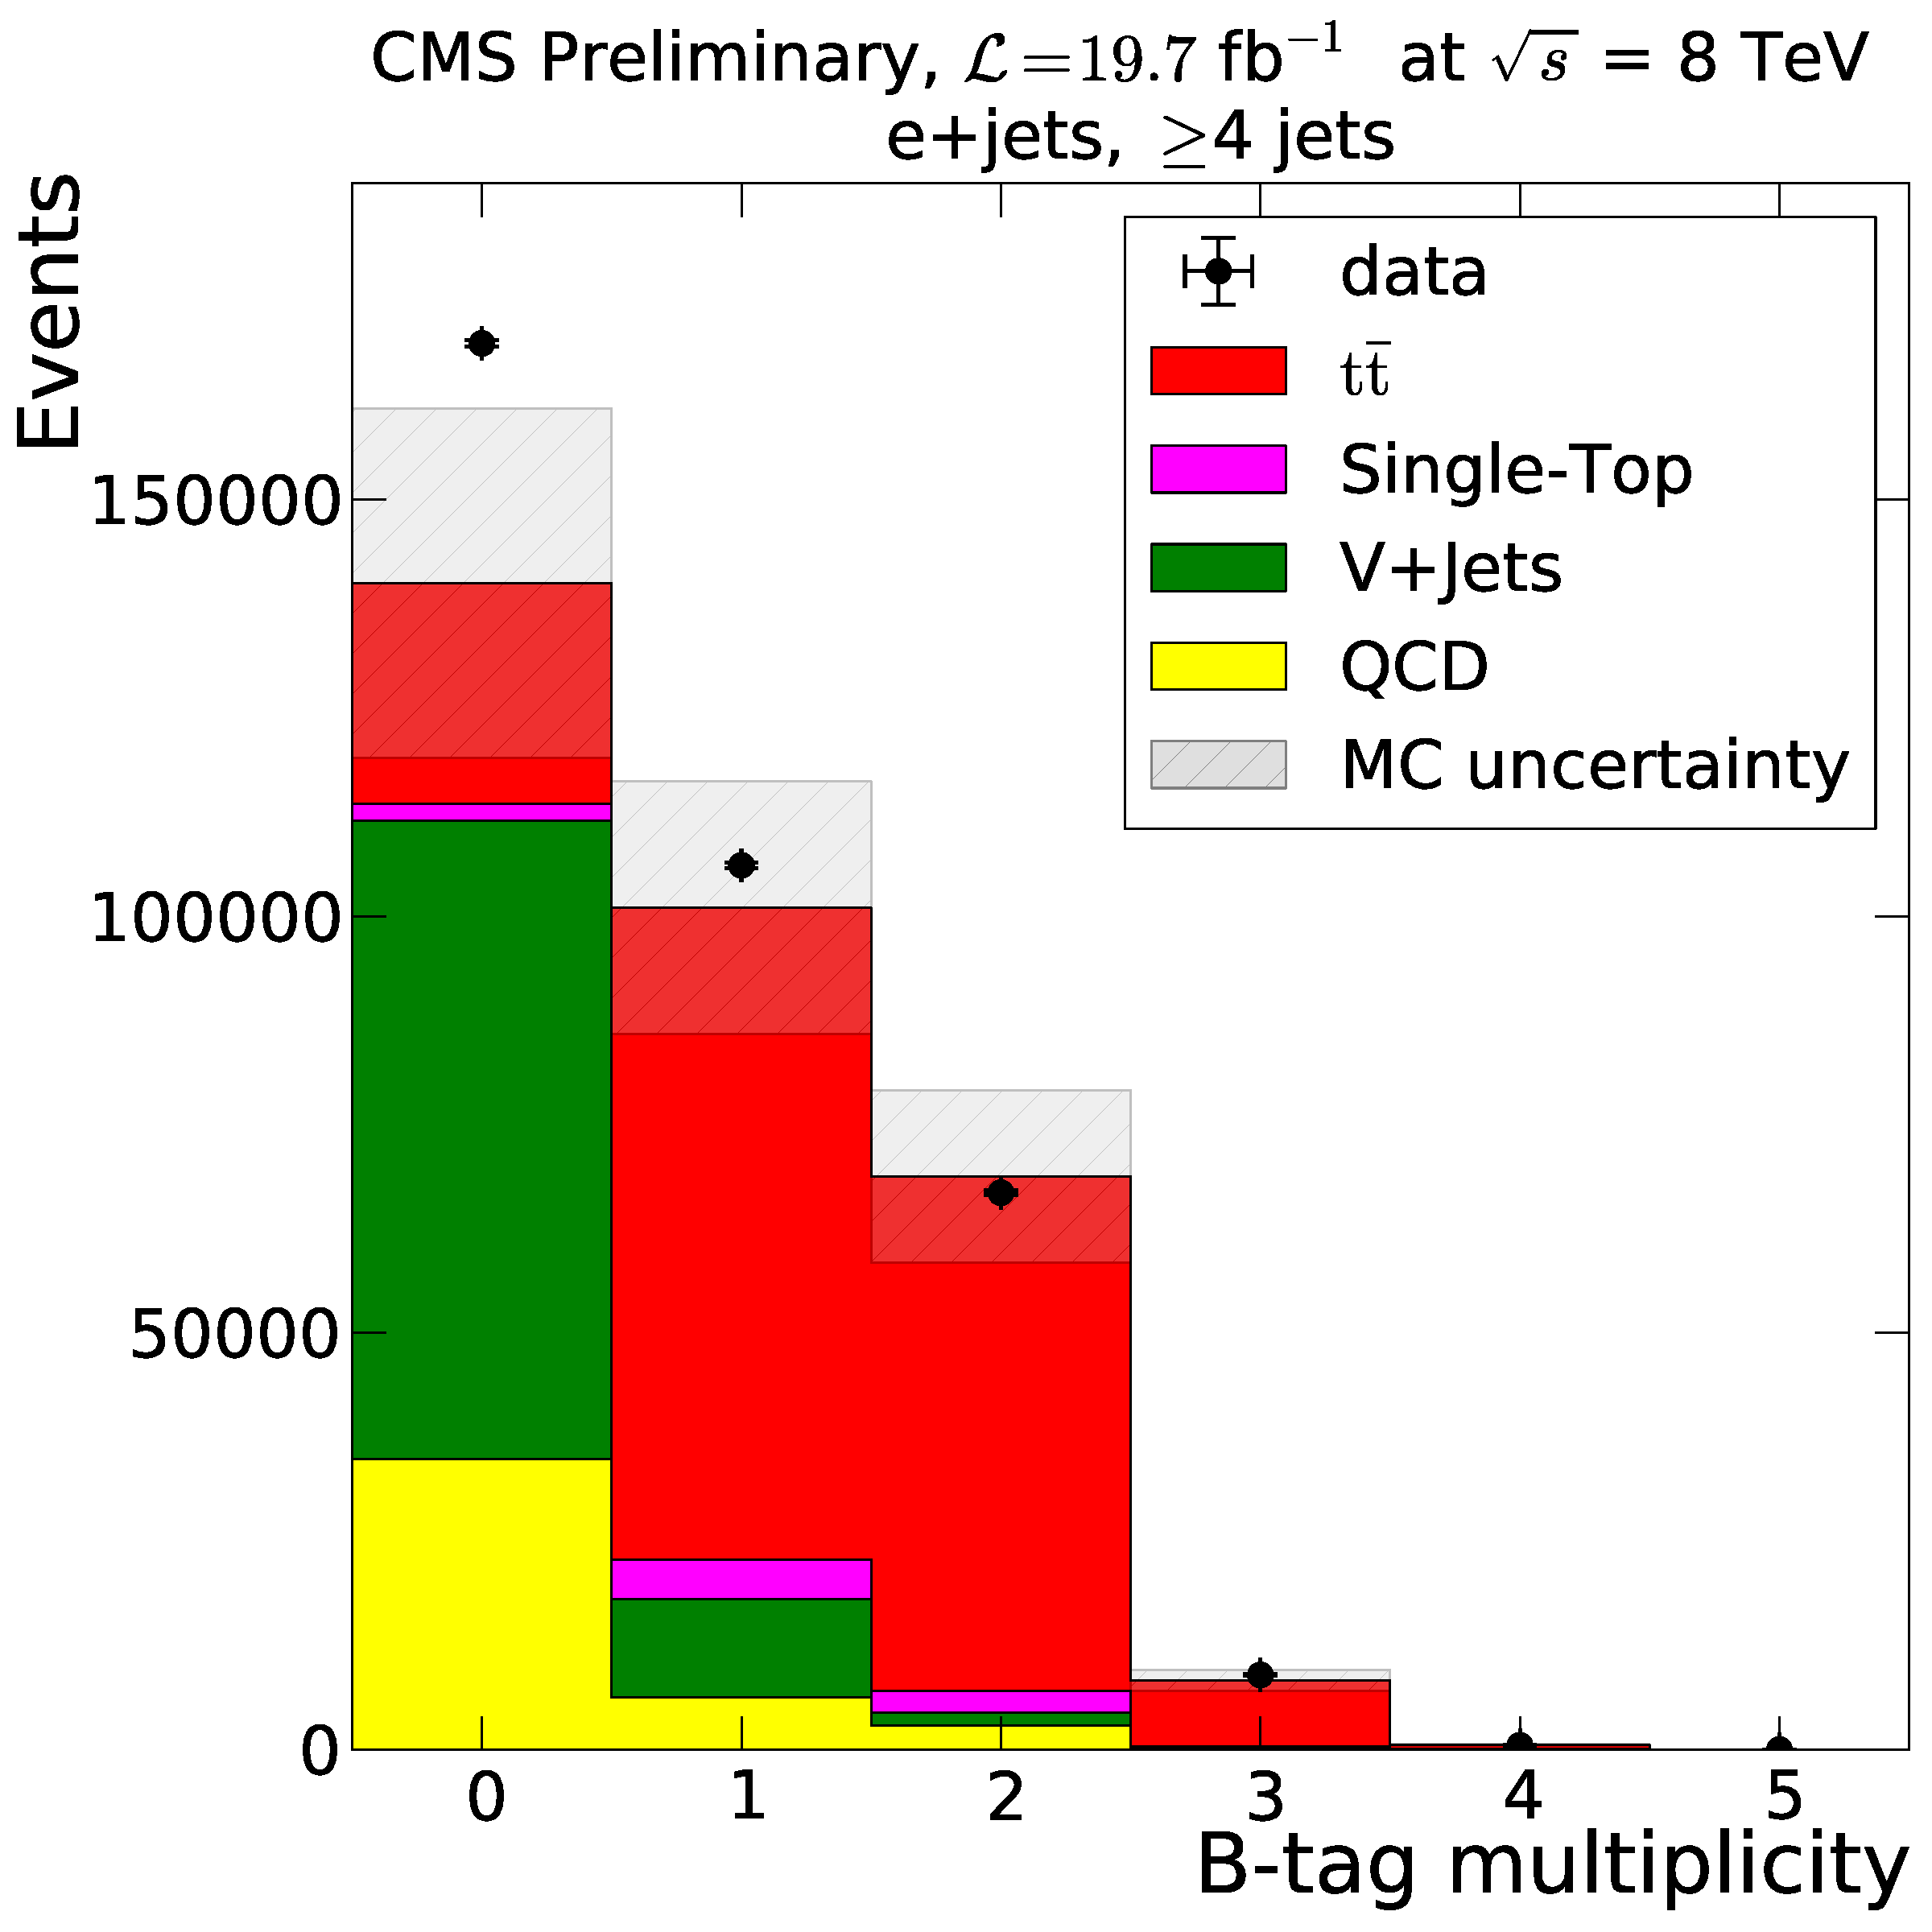
\includegraphics[width=0.50\textwidth]{bjets_multiplicity/EPlusJets_N_BJets_reweighted.pdf}} \\
	\subfloat[]{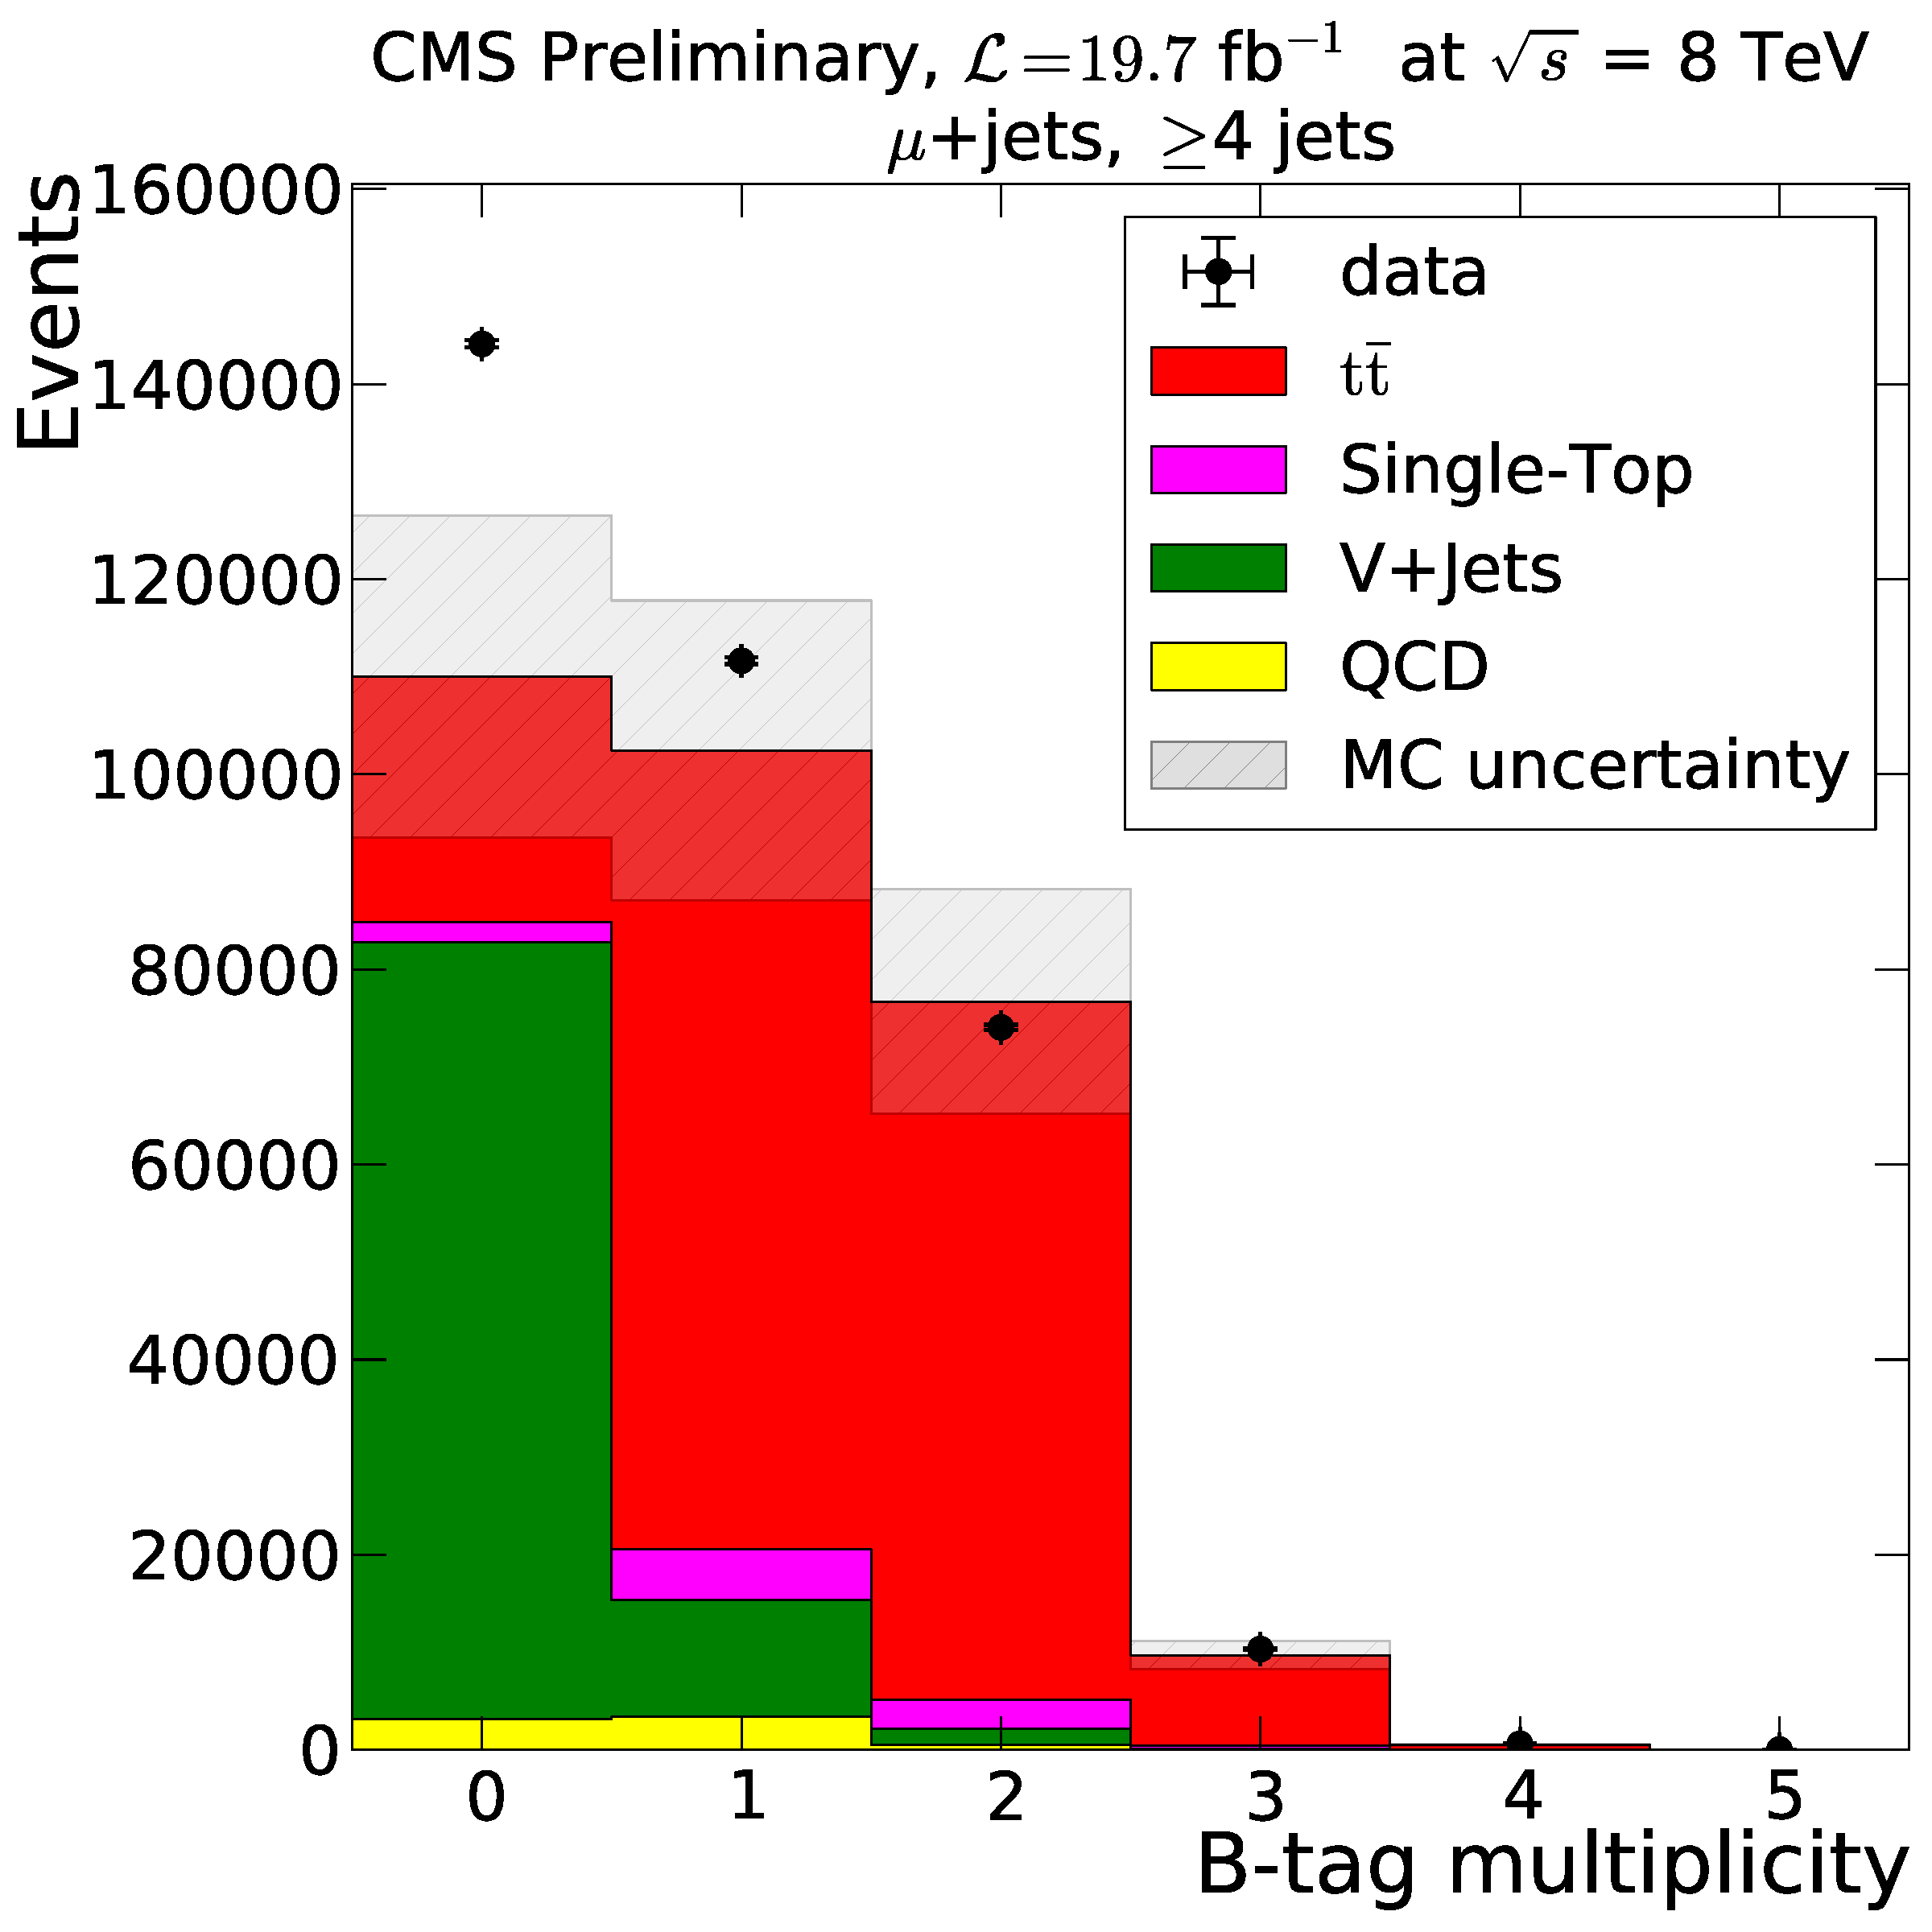
\includegraphics[width=0.50\textwidth]{bjets_multiplicity/MuPlusJets_N_BJets.pdf}}\hfill
	\subfloat[]{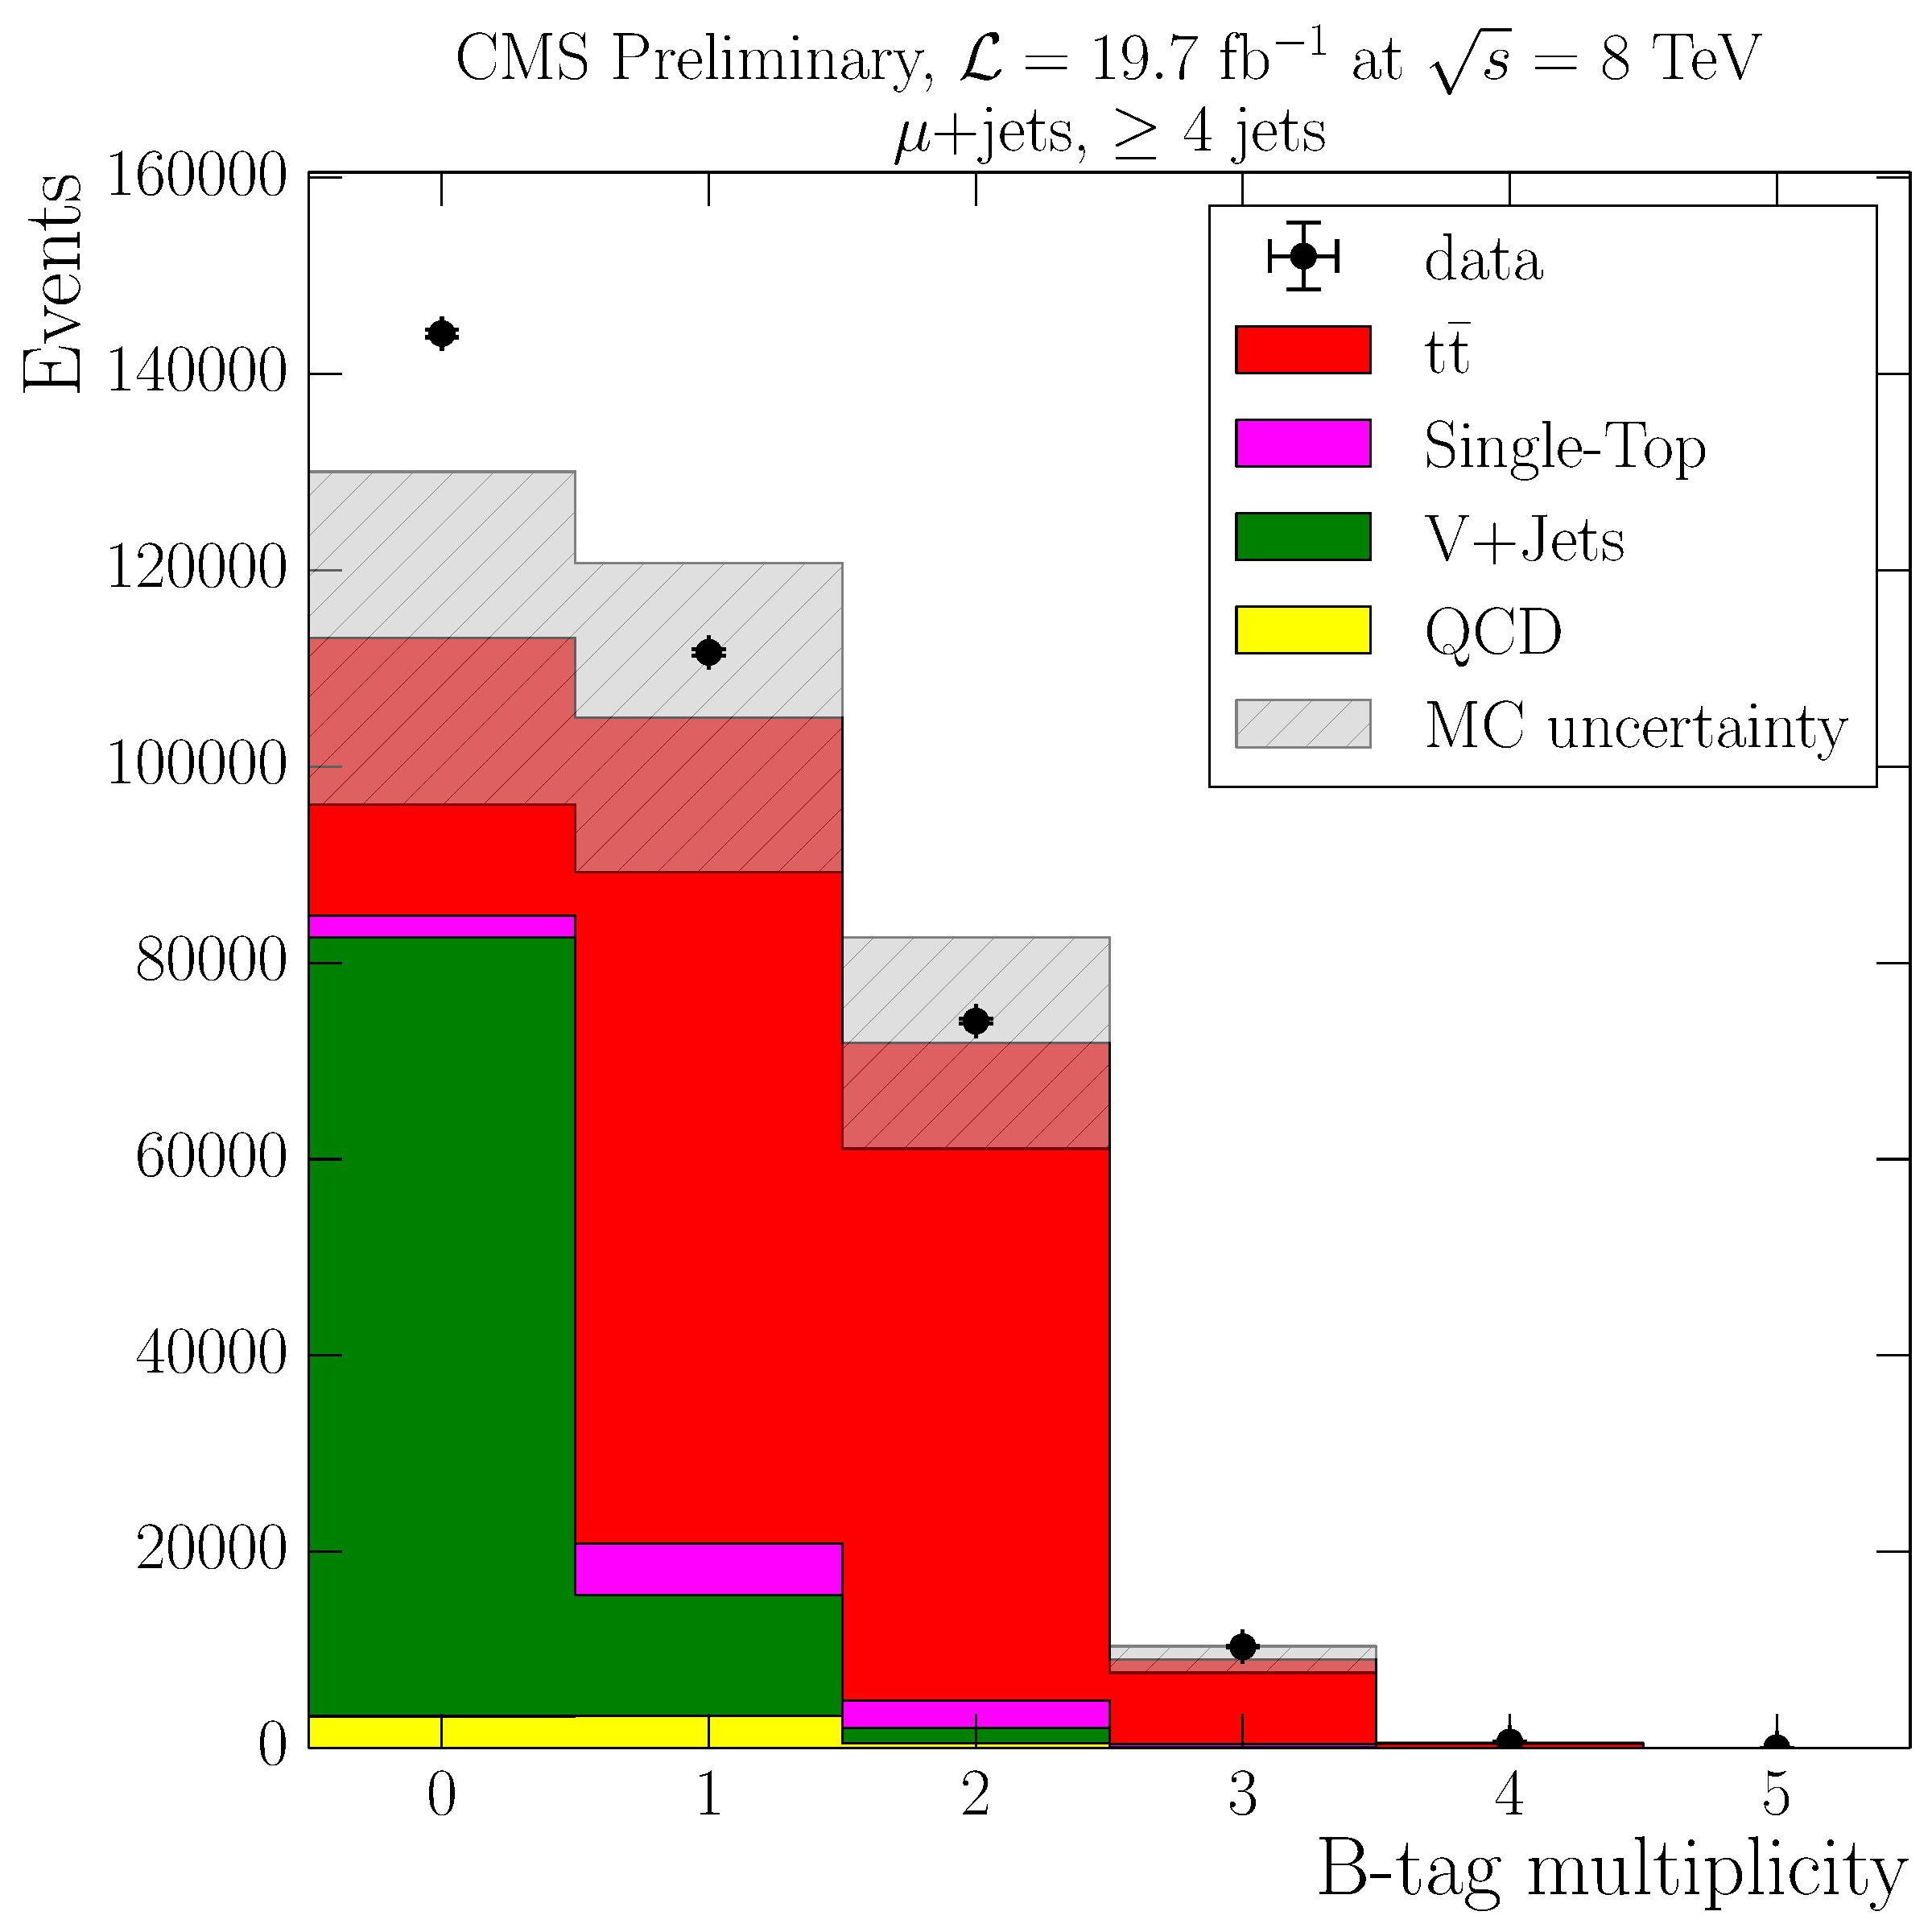
\includegraphics[width=0.50\textwidth]{bjets_multiplicity/MuPlusJets_N_BJets_reweighted.pdf}}
    \caption[b-tag multiplicity before and after applying the b-tagging scale factors]{b-tag multiplicity before (left)
    and after applying the b-tagging scale factors (right) in the electron channel (top) and the muon channel (bottom).}
    \label{fig:bjet_weights}
\end{figure}

Figure \ref{fig:bjet_weights} shows the results of the reweighting procedure for electron and muon channels. It can be
seen that the numbers of simulated events in b-tag multiplicity bins of \num{0} and \num{1} are scaled up, whereas for
other bins the number of MC events is scaled down. The systematic uncertainty due to b-tagging corrections is calculated
by applying $\pm 1 \sigma$ variations of the scale factors in the reweighting procedure.

\section{Event Selection}
\label{s_xsection:event_selection}
As in the top quark mass analysis, the event selection in this work is based on the standard CMS selection optimised for
Standard Model \ttbar production. It also exploits the semileptonic signature of a \ttbar decay with exactly one
isolated lepton and at least four jets, two of which are b-tagged. One of the main goals of the analysis is the
measurement of the missing transverse energy distribution represented by a neutrino from the leptonic decay of the \W
boson. However, there is no specific requirement on the \MET in the selection.

Comparing to the 2011 event selection described in Section~\ref{s_top_mass:event_selection}, enhanced pile-up
subtraction and lepton identification techniques are used. Improved understanding of the detector in form of updated
alignment and calibration constants resulted in better resolution of jets and \MET. The preselection (or skimming) step
used in order to reduce the number of events for local analysis processing is identical to that of the 2011 analysis.
However, additional filters are used to reject the events with artificial \MET caused by noise or known problems with
one of the detector subsystems. These filters are discussed in Section~\ref{ss_xsection:met_filters}.

Two semileptonic \ttbar decay modes are explored in this analysis: the electron plus jets and the muon plus jets
channels. The event selection for each of these decay modes is described below.

\subsection{Electron plus jets channel}
\label{ss_xsection:ejets}

Similarly to the electron plus jets channel in the top quark mass analysis, the selection consists of the following
steps:

\begin{enumerate}[topsep=\parskip, parsep=\parskip, itemsep=\parskip, leftmargin=\leftmargin]
	\item preselection;
	\item trigger;
	\item electron candidate selection;
	\item muon veto;
	\item dilepton veto;
	\item conversion veto;
	\item jet selection;
	\item b-tagging.
\end{enumerate}

%https://twiki.cern.ch/twiki/bin/view/CMS/TWikiTop2011DataMCTrig

\subsubsection*{Trigger}
In contrast to the 2011 analysis using cross triggers, a single electron trigger is used in this analysis. Referred to
as HLT\_Ele27\_WP80, this trigger has a lepton \pt threshold of \SI{27}{\GeV} and ``WP80'' lepton isolation requirement
(see Table~\ref{tab:trigger_naming}), but no specific jet requirements. In 2012, the single electron trigger was
unprescaled for the whole running period, despite a comparatively large rate. The decision to keep the trigger
unprescaled was made due to simplicity of the trigger selection, requiring flat efficiency corrections.

\subsubsection*{Electron candidate selection}
Similarly to 2011 selection, exactly one electron candidate passing is required in the event, passing the following
criteria:

\begin{itemize}
	\item $\ET > \SI{30}{\GeV}$;
	\item $|\eta| < 2.5$, excluding the ECAL barrel-endcap transition regions of $1.4442 < |\eta| < 1.566$;
	\item MVA electron ID (Section~\ref{ss:electron_reconstruction}) with a discriminator cut of $>0.5$;
	\item transverse impact parameter with respect to the primary vertex $d_{xy} < \SI{0.02}{\cm}$;
	\item PF-based relative isolation (Section~\ref{sss:electron_isolation}) \reliso $< 0.1$ with a $\Delta
R$ cone of \num{0.3}.
\end{itemize}

\subsubsection*{Muon veto}
To reduce contamination from other \ttbar decay modes (i.e.\ muon and dilepton channels), events containing a global or
a tracker muon (see Section \ref{ss:muon_reconstruction}) are rejected. The requirements on the muon are identical to
those of 2011 selection: $\pt > \SI{10}{\GeV}$, $|\eta| < 2.5$ and $\reliso < 0.2$ with a $\Delta R$ cone of \num{0.4}.

\subsubsection*{Dilepton veto}
To reject events with additional electrons, a dilepton veto is applied. Events are rejected if they contain a second
electron candidate with the same ID and $\eta$ requirements, but looser \ET and \reliso criteria ($>\SI{20}{\GeV}$ and
$<0.15$, respectively).

\subsubsection*{Conversion veto}
As described in Section~\ref{sss:photon_conversions}, a vertex fit technique combined with the number of missing hits
in the tracker is used for photon conversion rejection.

\subsubsection*{Jet selection and b-tagging}
To help further reduce the background, at least four jets with $\pt > \SI{30}{\GeV}$ and $|\eta| < 2.5$ are required in
the event. These jets are required to pass the loose PF jet ID (see Section \ref{ss:jet_reconstruction}). Before the
multiplicity and identification requirements, the collection of jets is cleaned against the signal electron, i.e.\ any
jet within a $\Delta R$ cone of \num{0.3} around the signal lepton is excluded from the analysis. This is done due to
the fact that an electron may be reconstructed as a jet by leaving a characteristic signature in calorimeters. Any
additional jets with $\pt > \SI{20}{\GeV}$ and the same cleaning and ID requirements are also used for calculation of
\HT and \ST variables (Section~\ref{ss_xsection:variables}). Finally, the combined secondary vertex (CSV) b-tagging
algorithm with the medium working point (Section \ref{sss:b-tagging}) is used to identify the jets originating from
\cPqb-quarks in the \ttbar decay. At least two b-tagged jets are required in this analysis.

\subsection{Muon plus jets channel}
\label{ss_xsection:mujets}
The muon channel event selection follows a strategy similar to that of the electron channel:

\begin{enumerate}[topsep=\parskip, parsep=\parskip, itemsep=\parskip, leftmargin=\leftmargin]
	\item preselection;
	\item trigger;
	\item muon candidate selection;
	\item second muon veto;
	\item electron veto;
	\item jet selection;
	\item b-tagging.
\end{enumerate}

\subsubsection*{Trigger}
An isolated single muon trigger, referred to as HLT\_IsoMu24\_eta2p1, is used in this channel. Partially suggested by
the name of the trigger path, the following criteria on the muon are imposed at the HLT level:

\begin{itemize}
	\item $\pt > \SI{24}{\GeV}$;
	\item $\abs \eta < 2.1$;
	\item Combined tracker and calorimeter-based relative isolation (Section~\ref{sss:electron_isolation}) \reliso $<
0.15$ with a $\Delta R$ cone of 0.3.

% according to https://twiki.cern.ch/twiki/bin/viewauth/CMS/MuonHLT isolation used to be 0.1, dR=0.24 in RunA
\end{itemize}

\subsubsection*{Muon candidate selection}
For selection of a muon candidate, exactly one muon satisfying the following requirements is required:

\begin{itemize}
	\item $\pt > \SI{26}{\GeV}$;
	\item $|\eta| < 2.1$;
	\item PF-based relative isolation (Section~\ref{sss:electron_isolation}) \reliso $< 0.12$ with a $\Delta
R$ cone of \num{0.4};
	\item PF-muon ID criteria (Section \ref{ss:muon_reconstruction}):
	\begin{itemize}
		\item identified as a particle flow muon and as a global muon;
		\item a normalised of the global muon fit $\chi^2<10$;
		\item number of muon chamber hits $>0$;
		\item number of muon stations with muon segments $>1$;
		\item transverse impact parameter w.r.t. the primary vertex $d_{xy} < \SI{0.02}{\cm}$;
		\item longitudinal distance of the tracker track w.r.t. the primary vertex $d_z < \SI{0.5}{\cm}$;
		\item number of hits in the pixel detector $>0$;
		\item number of hits in the tracker layers $>5$.
	\end{itemize}
\end{itemize}

\subsubsection*{Second muon veto}
Events containing an additional loose muon are rejected, with loose ID requirements as follows:

\begin{itemize}
	\item $\pt > \SI{10}{\GeV}$;
	\item $|\eta| < 2.5$;
	\item PF-based relative isolation (Section~\ref{sss:electron_isolation}) \reliso $< 0.2$ with a $\Delta R$ cone of
	\num{0.4}; %PU corrections!
	\item identified as a particle flow muon, and either global or tracker muon.
\end{itemize}

These criteria are identical to the muon veto requirements in the electron channel.

\subsubsection*{Electron veto}
To further reduce background contamination, events with electrons are rejected. The requirements on additional loose
electron are the same to the dilepton veto in the electron channel.

\subsubsection*{Jet selection and b-tagging}
Finally, the jet requirements are applied. These are also identical to those of the electron channel, mentioned above.


\subsection{Additional filters for missing transverse energy}
\label{ss_xsection:met_filters}
%https://twiki.cern.ch/twiki/bin/viewauth/CMS/MissingETOptionalFilters

There is no specific requirement on missing transverse energy in the selection, however, a set of corrections is applied
to \MET. As described in Section~\ref{ss:MET_reconstruction}, jet energy corrections are propagated to \MET, and it is
also corrected for pile-up and various detector effects causing $\phi$ modulation.

Additionally, a set of optional filters, prescribed for analyses with high sensitivity to \MET, was applied in the
selection for both electron and muon channels. Most of these filters were put in place after discovering events with
anomalously high missing transverse energy. A short description of each filter is given below.

\begin{description}[wide=\parindent]
	\item[CSC beam halo filter.]
	Protons in the LHC beams can interact with residual particles of beam collimators, which produces secondary particle
	showers referred to as beam halo \autocite{beam_halo_CMS}. This machine-induced background can significantly
	contaminate collision events, particularly affecting the \MET observable due to specific trajectories of halo muons.
	A dedicated algorithm based on exploiting the halo signatures in the Cathode Strip Chambers (CSCs) helps to mitigate
	this background.

	\item[HCAL laser filter.] The HCAL laser system is used for calibration and monitoring the detector response
	\autocite{CMS_TDR1}. During the 2012 data-taking, laser pulses were accidentally fired and consequently polluted a
	small fraction of the recorded physics dataset. Using the fact that unlike physics events, laser pulses produce hits
	in calibration channels of the HCAL, the dataset is filtered from this contamination.
	%https://indico.cern.ch/event/169318/contribution/1/material/slides/0.pdf

	\item[ECAL dead cell filter.] Both ECAL endcap and barrel regions are known to have faulty crystals producing too
	much noise in detector readouts. There are also crystals corresponding to front-end cards with defective data link.
	All these channels are masked in reconstruction and constitute to about \SI{1}{\pc} of the total amount. However,
	they can still cause a significant amount of energy deposits to be lost, therefore contributing to fake \MET. One of
	the approaches to tackle this issue uses the so-called trigger primitive information, i.e.\ digital quantities
	produced by the Level 1 trigger electronics \autocite{CMS_L1_Trigger_TDR}. Another approach uses the energy deposits
	surrounding the masked channels (boundary energy). These methods allow to filter events with the estimated energy
	leakage above certain threshold (\SI{\sim10}{\GeV}).
	%https://twiki.cern.ch/twiki/bin/viewauth/CMS/SusyEcalMaskedCellSummary

	\item[Tracking failure filter.] Some events have been observed to have a lack of tracks corresponding to standard or
	large calorimeter deposits. There are two understood sources of this misreconstruction: in a first type of such
	events, the tracking algorithm (explained in Section~\ref{ss:electron_reconstruction}) halts for some of its
	iterations due to an exceeding number of calorimeter clusters. In a second type the hard collision happens in a
	satellite colliding bunch at a distance of approximately \SI{75}{\cm} from the nominal interaction point along the
	$z$ axis. A cut on the summed \pt of the tracks originating from the primary vertices passing the preselection
	criteria, divided by the summed \pt of all jets in the event, was found to clearly distinguish between pathological
	and unaffected events. A cut value of \SI{10}{\pc} is imposed.
	%https://twiki.cern.ch/twiki/bin/viewauth/CMS/SusyRA2NJetsInData2010#Tracking_failure

	\item[Bad ECAL endcap super-cluster filter.] In 2012, two $5\times5$ super-clusters in the ECAL endcap regions were
	observed to occasionally produce anomalous pulses, leading to artificially high \MET. The source of this issue can
	be related to the High-Voltage system, but is subject to further investigation. A filter removing the problematic
	events is used, configured to cut on the total energy of reconstructed hits not passing the nominal quality criteria
	in the two super-clusters, with the cut value of \SI{1}{\TeV}.
	%https://twiki.cern.ch/twiki/bin/viewauth/CMS/MissingETOptionalFilters#Bad_EE_Supercrystal_filter_added

	\item[ECAL laser correction filter.] Lead tungstate crystals of the ECAL naturally lose their transparency with
	radiation exposure. To maintain high precision, this effect is corrected for by frequently injecting laser pulses
	and reading out the response in order to calibrate each crystal \autocite{CMS_TDR1}. During 2012 data-taking, a
	handful of crystals had unphysically large values of laser corrections, resulting in anomalously high \MET in
	recorded events. The filter removes such events from the dataset.
	%https://twiki.cern.ch/twiki/bin/viewauth/CMS/PdmVKnowFeatures#Filter_to_reject_events_with_ano

	\item[Strip tracker noise filter.] A few events were affected by a large coherent noise in the silicon strip
	tracker, which resulted in a much larger number of the strip clusters compared to according pixel cluster
	multiplicity in the tracking algorithm. A dedicated filter rejects events with this anomaly.
	%https://twiki.cern.ch/twiki/bin/viewauth/CMS/TrackingPOGFilters#Filters

\end{description}

% Although the number of events removed by these filters is extremely small (\SI{\ll1}{\pc}), most of them have high
% fake \MET, which could lead to an artificial excess in the \MET distribution. Due to the analysis sensitivity to
% \MET, application of these filters was rather important.

\section{Data-driven QCD estimation}
\label{s_xsection:data_driven_QCD}
QCD multi-jet events constitute an important background to semileptonic \ttbar decays, and one of the most difficult to
model (Section~\ref{ss:backgrounds}). The requirement of two b-tagged jets in the event selection is mainly motivated by
the necessity to mitigate the effect of this particular background. In this analysis, the final QCD yield is obtained
from the fitting process as explained in Section~\ref{s_xsection:measurement}. However, the initial estimate is
performed using data-driven techniques. Only the shape of the distribution is of importance here as the normalisation is
determined in the fitting process. The QCD estimation methods for both electron and muon channel are described in detail
hereafter.

\subsection{QCD multi-jet events with electrons}
Two control regions have been investigated in the electron channel:

\begin{itemize}
\item conversion control region: conversion veto is inverted in the full event selection;
\item non-isolated electron control region: the electron isolation requirement is changed from $\reliso < 0.1$ to
$\reliso > 0.2$.
\end{itemize}

Additionally, only events with no b-tagged jets are taken into account to increase the statistics and QCD purity in both
control regions. In Figure~\ref{fig:qcd_control_regions_eta} the distributions of the absolute pseudorapidities of the
electron are presented for both control regions. The distributions observed in data are compared with MC expectations.
It can be seen that the distributions are not well described by the Monte Carlo, e.g.\ occasional high peaks in the QCD
MC represent the lack of statistics in simulation. Moreover, the two control regions have considerably different shapes
in the electron $\abs \eta$ distributions. For the conversion control region, the shape is mostly flat in the barrel
region ($\abs \eta < 1.5$) and peaks in the endcap region ($\abs \eta > 1.5$), which is expected as the conversions are
more likely to happen in the region with higher material budget. In contrast, the non-isolated control region peaks in
the pseudorapidity region of $1.0 < \abs \eta < 1.5$. Such behaviour is correlated with the jet $\abs
\eta$ distribution, since this control region favours non-isolated electrons coming from heavy quark decays.

\begin{figure}[htbp]
	\centering
  	\subfloat[]{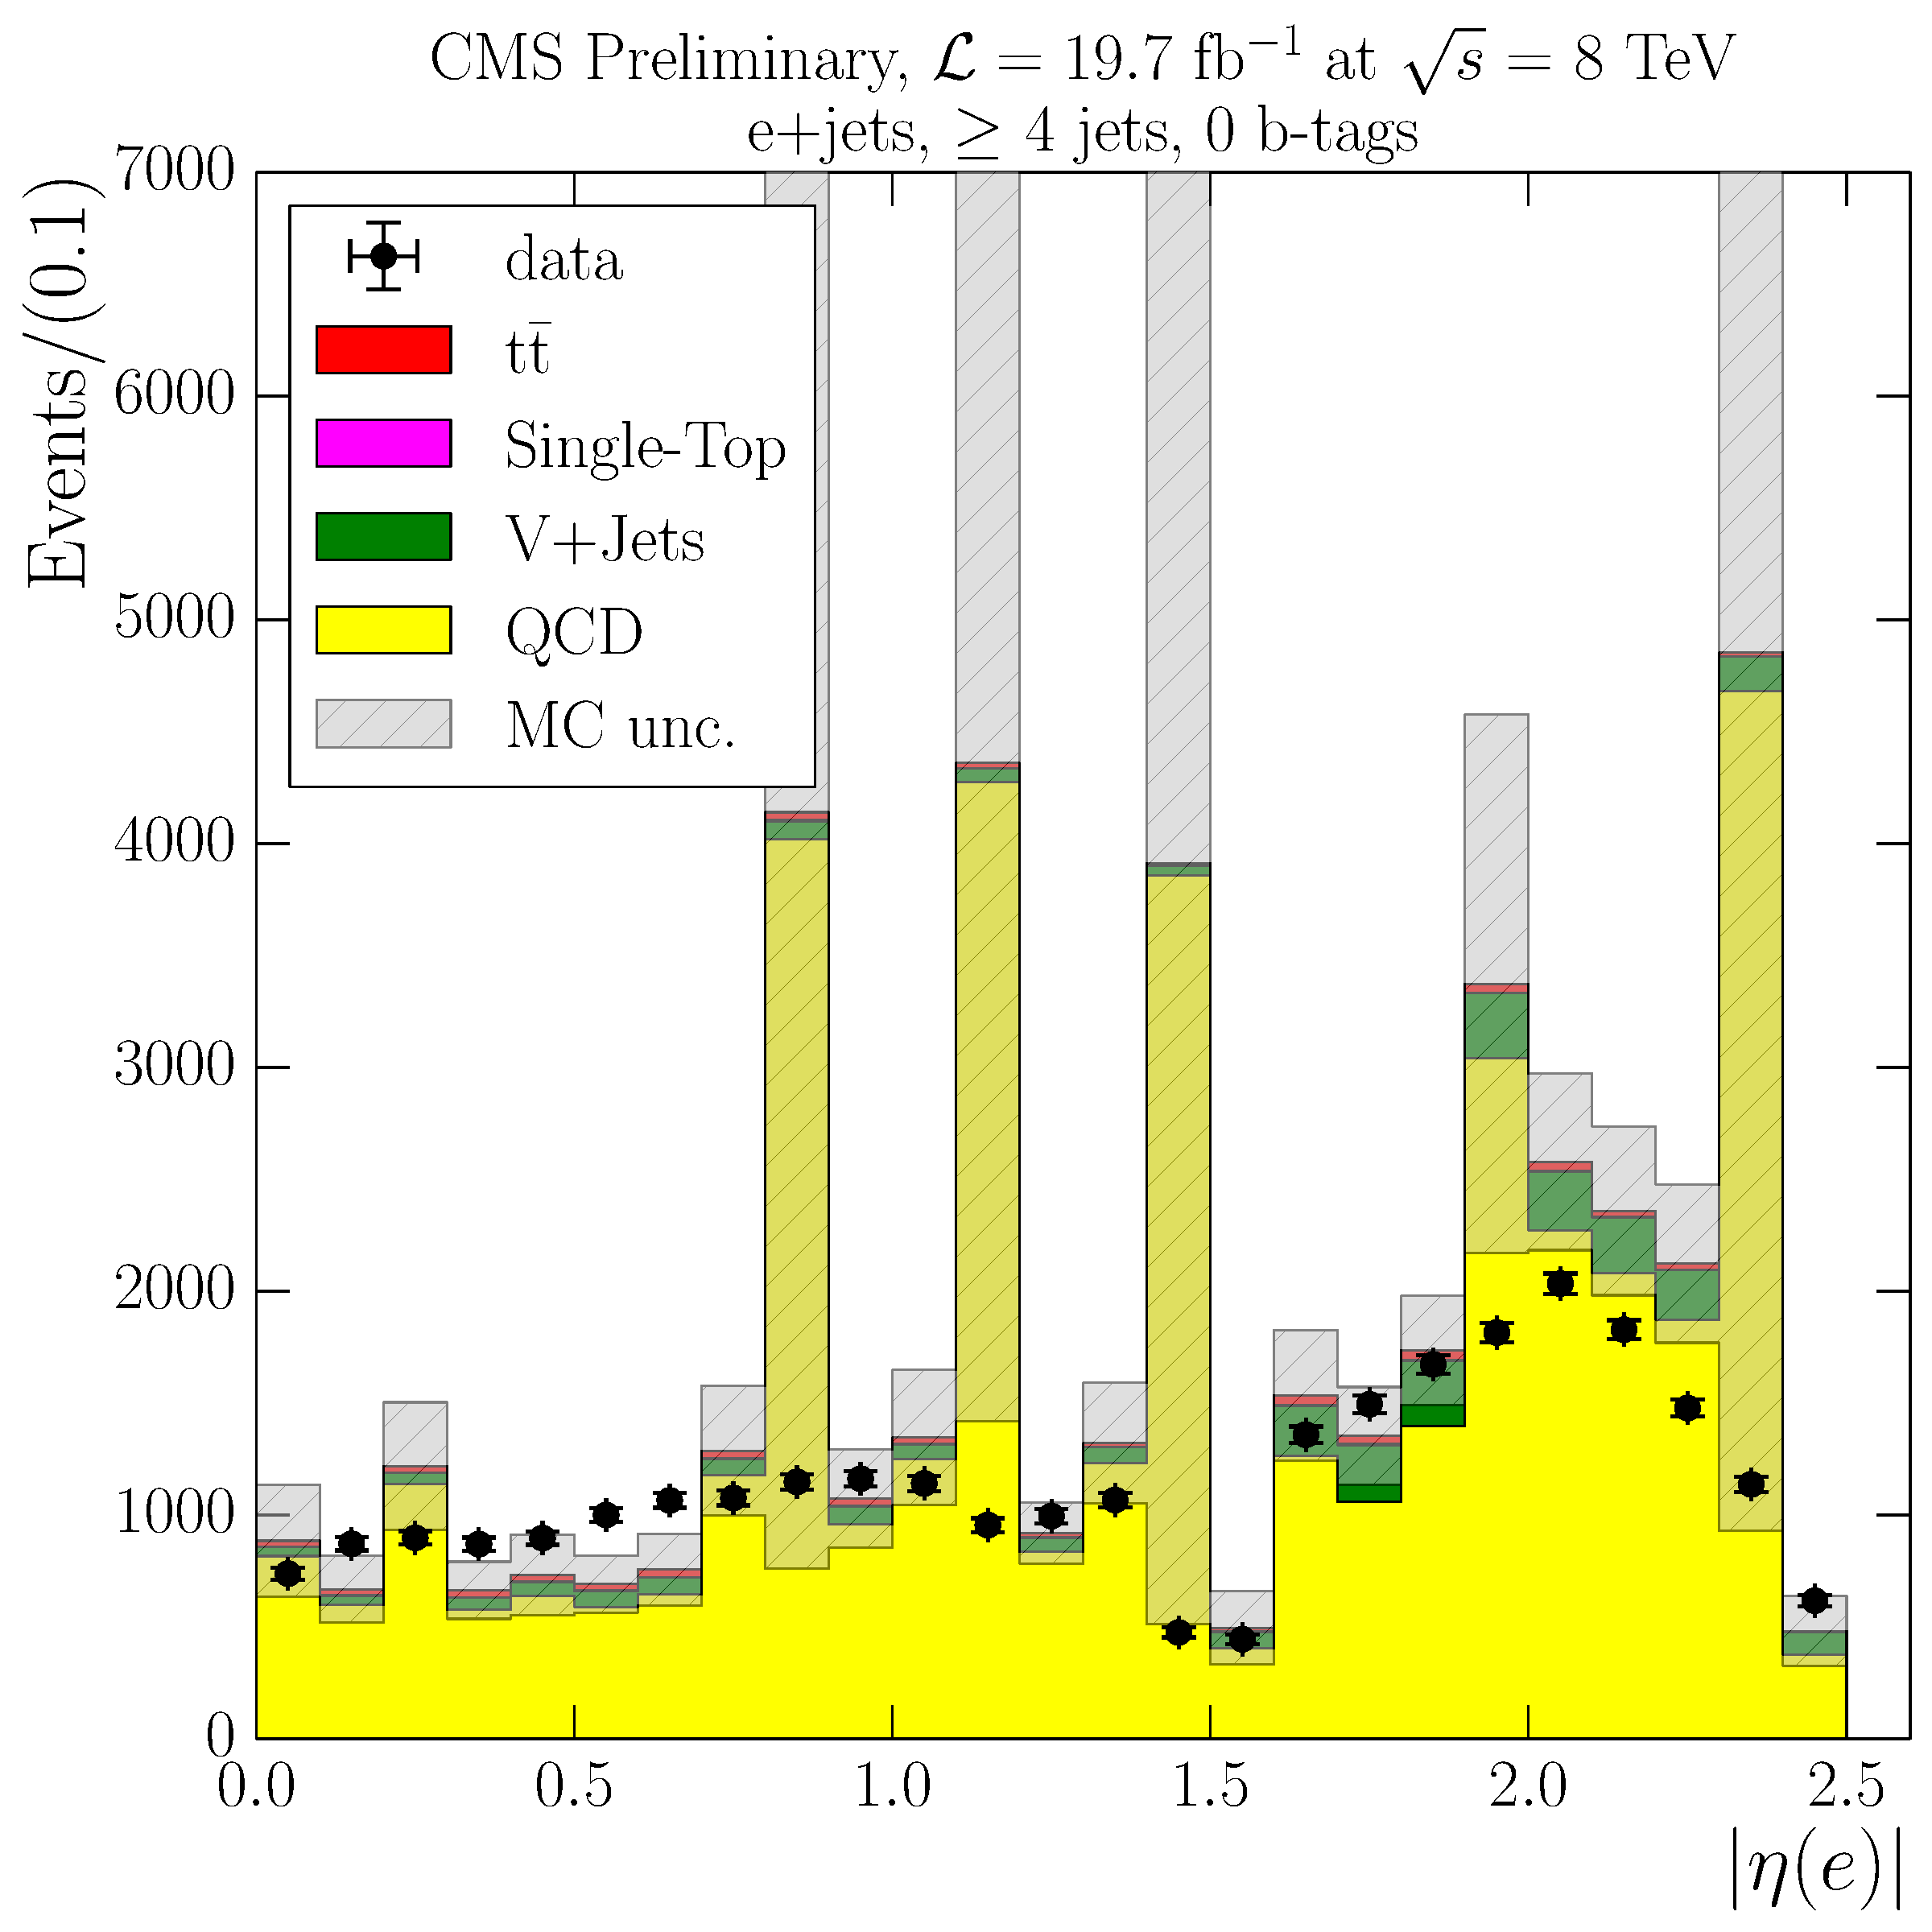
\includegraphics[width=0.50\textwidth]{QCD/QCD_conversion_control_region_electron_AbsEta_0btag}}\hfill
	\subfloat[]{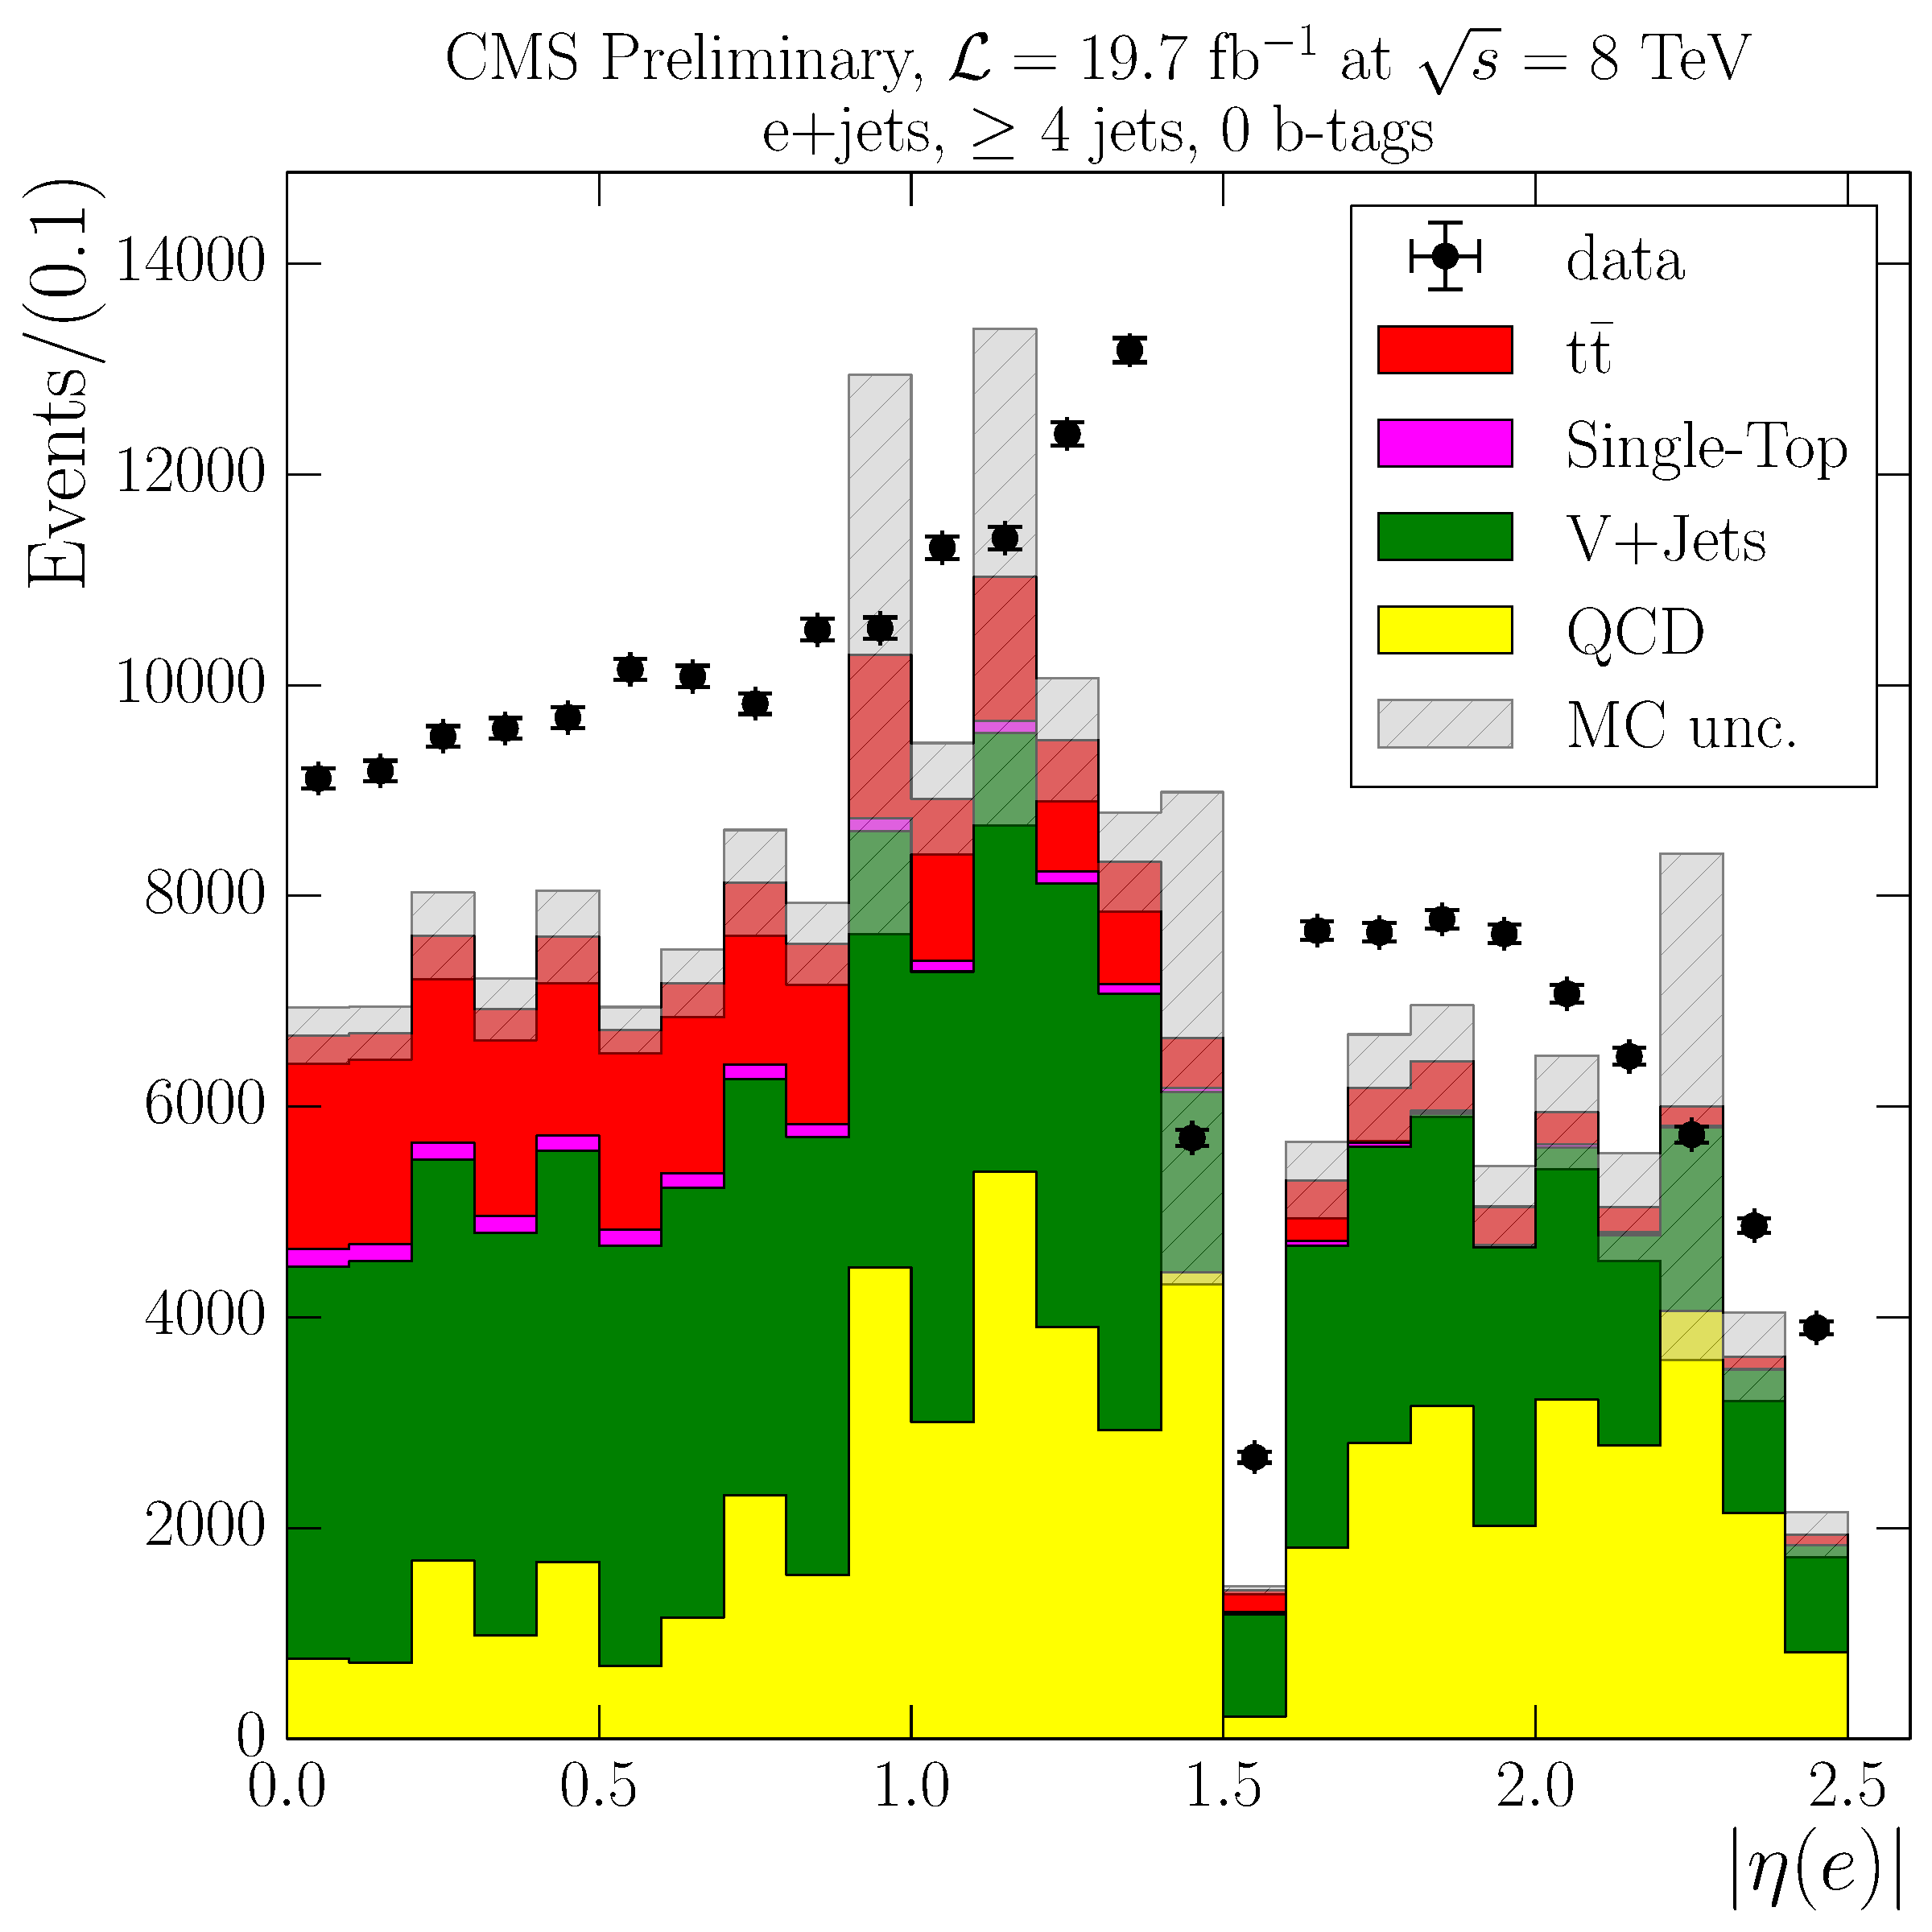
\includegraphics[width=0.50\textwidth]{QCD/QCD_non_iso_control_region_electron_AbsEta_0btag}} \\
	\subfloat[]{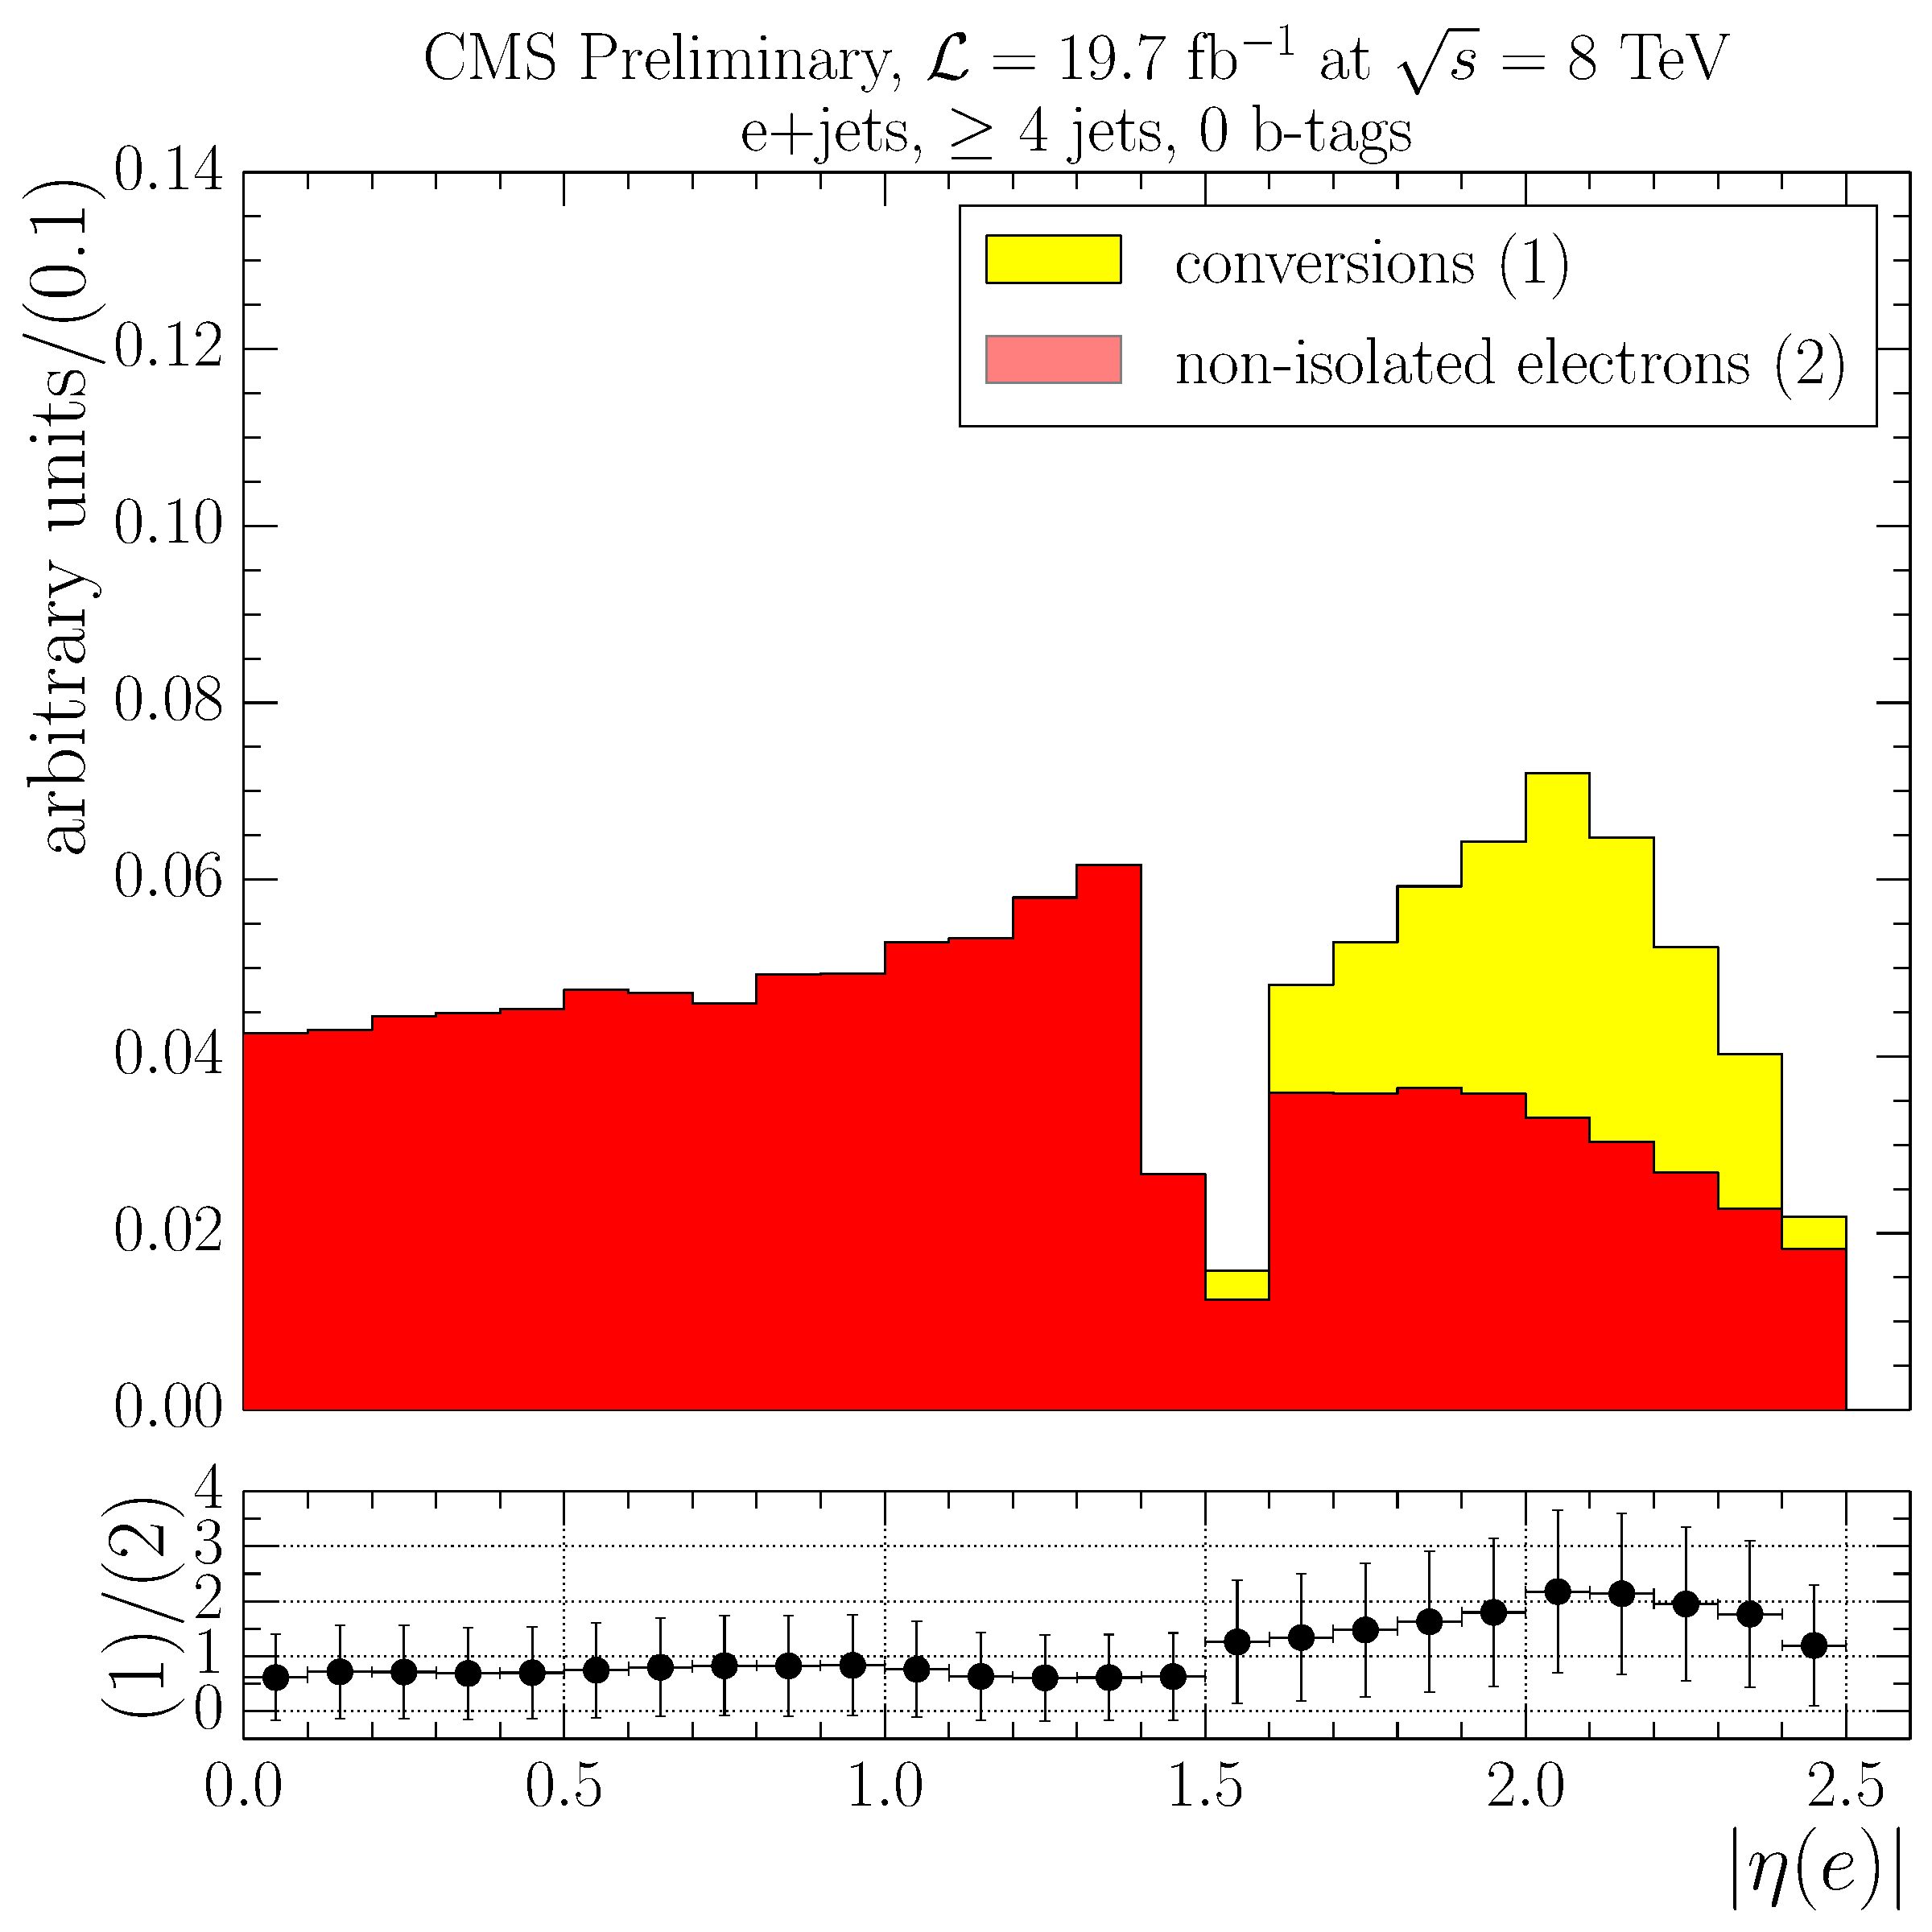
\includegraphics[width=0.50\textwidth]{QCD/QCD_control_region_comparison_electron_AbsEta_0btag}}
    \caption[Distribution of the electron $\abs \eta$ for conversion selection and non-isolated electron selection, and
    the shape comparison of both QCD control regions]{Distribution of the electron $\abs \eta$ for conversion selection
    (a), non-isolated electron selection (b) and the shape comparison of both QCD control regions in data (c) in
    electron plus jets events with at least four jets and 0 b-tagged jets.}
    \label{fig:qcd_control_regions_eta}
\end{figure}

Also, in Figure~\ref{fig:qcd_control_regions_eta} we see that while the conversion region is predicted to be a rather
pure QCD sample, the non-isolated control region has significant contamination from \ttbar signal and \W/\ZpJets events.
For this reason, the conversion region was chosen to produce the QCD template for the electron channel. However, since
the relative contributions of the QCD events from both control regions in the final selected sample are not known, the
real QCD shape can differ considerably from the prediction. Therefore, the non-isolated region is used to estimate the
systematic uncertainty due to the QCD shape choice. This systematic error is estimated by substituting the nominal QCD
template from the conversion control region with that from the non-isolated region, and calculating the change in the
final measurement. More information on systematic uncertainties is presented in Section~\ref{s_xsection:systematics}.

\subsection{QCD multi-jet events with muons}
For the QCD shape extraction in the muon plus jets channel, the inverted isolation cut is applied in the event
selection: at least one muon with $\reliso>0.3$ is required, and events with isolated muons with $\reliso<0.3$ are
vetoed. Similarly to the electron channel, only events with no b-tagged jets are taken into account. Additionally, to
increase the available statistics, events with only three jets are also considered ($\geq 3$ jet bin).

The relative isolation distribution with the cut value and the muon $\abs \eta$ for the non-isolated region are shown on
Figure~\ref{fig:qcd_muon_plots}. Clearly, the control region is dominated by QCD events and generally there is a
reasonable agreement between data and simulation. The contamination from other processes is subtracted using Monte
Carlo.

\begin{figure}[!htbp]
	\centering
  	\subfloat[]{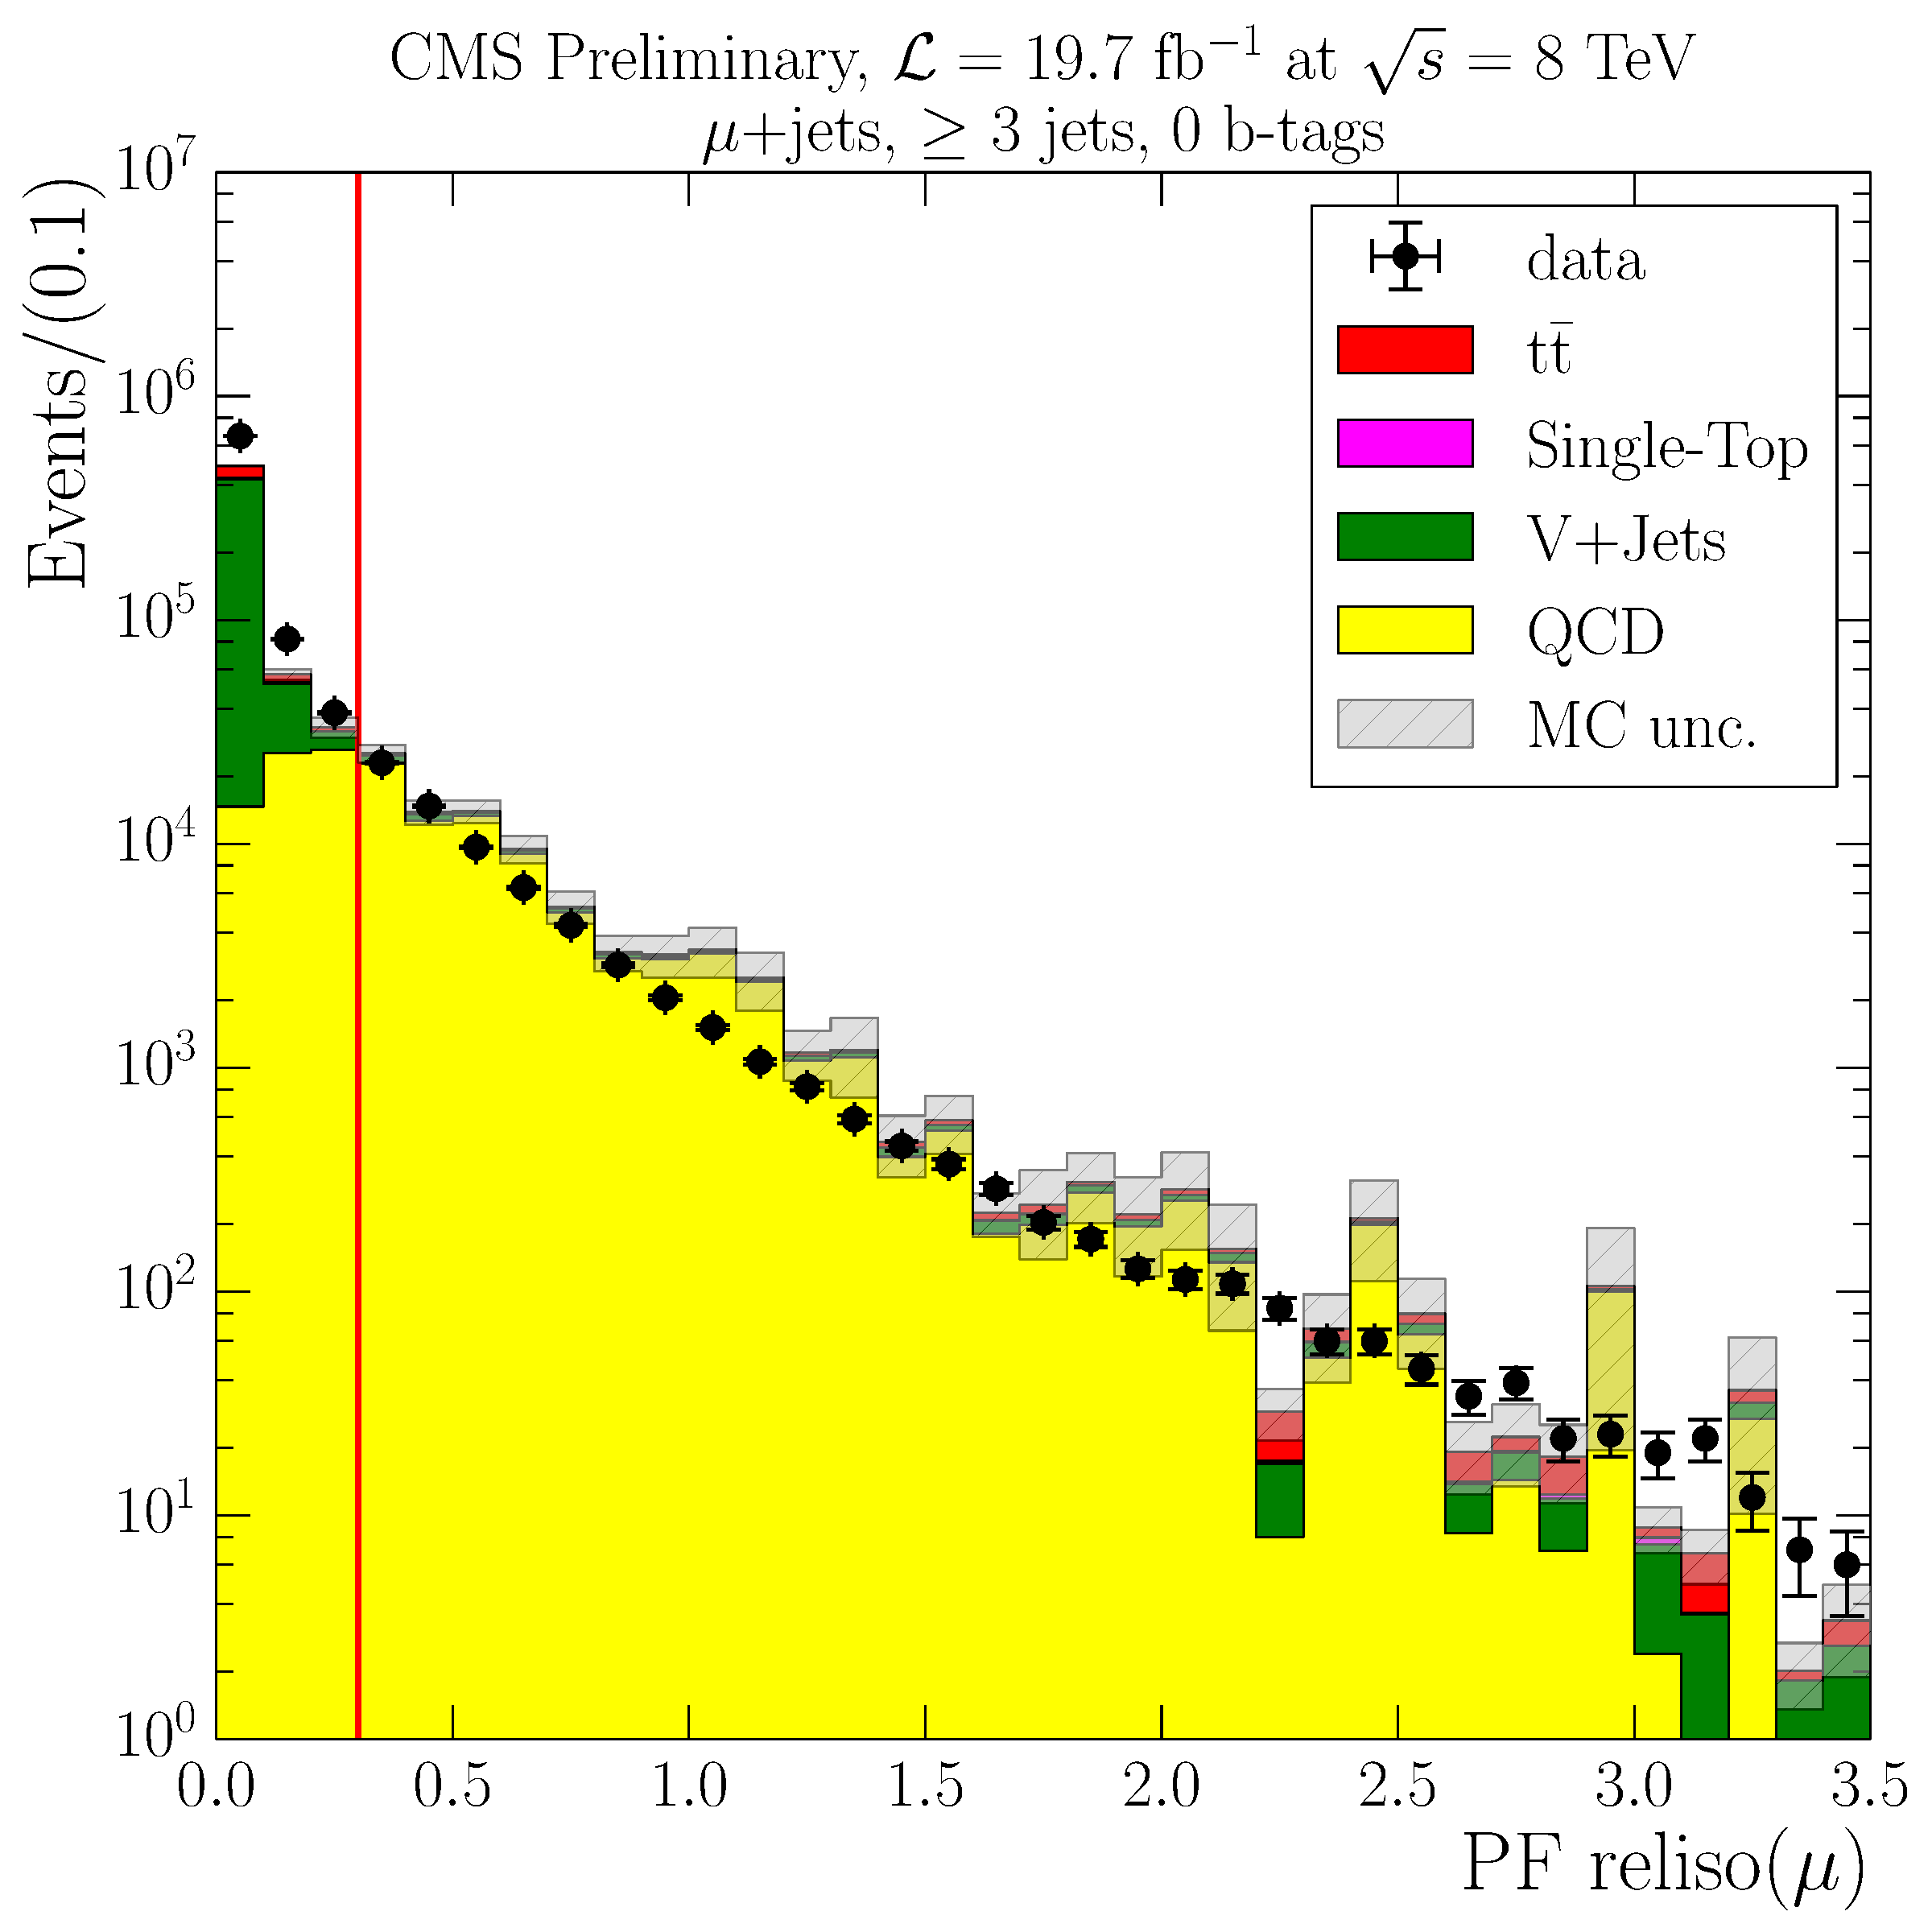
\includegraphics[width=0.47\textwidth]{QCD/QCD_muon_pfIsolation_0btag}}\hfill
  	\subfloat[]{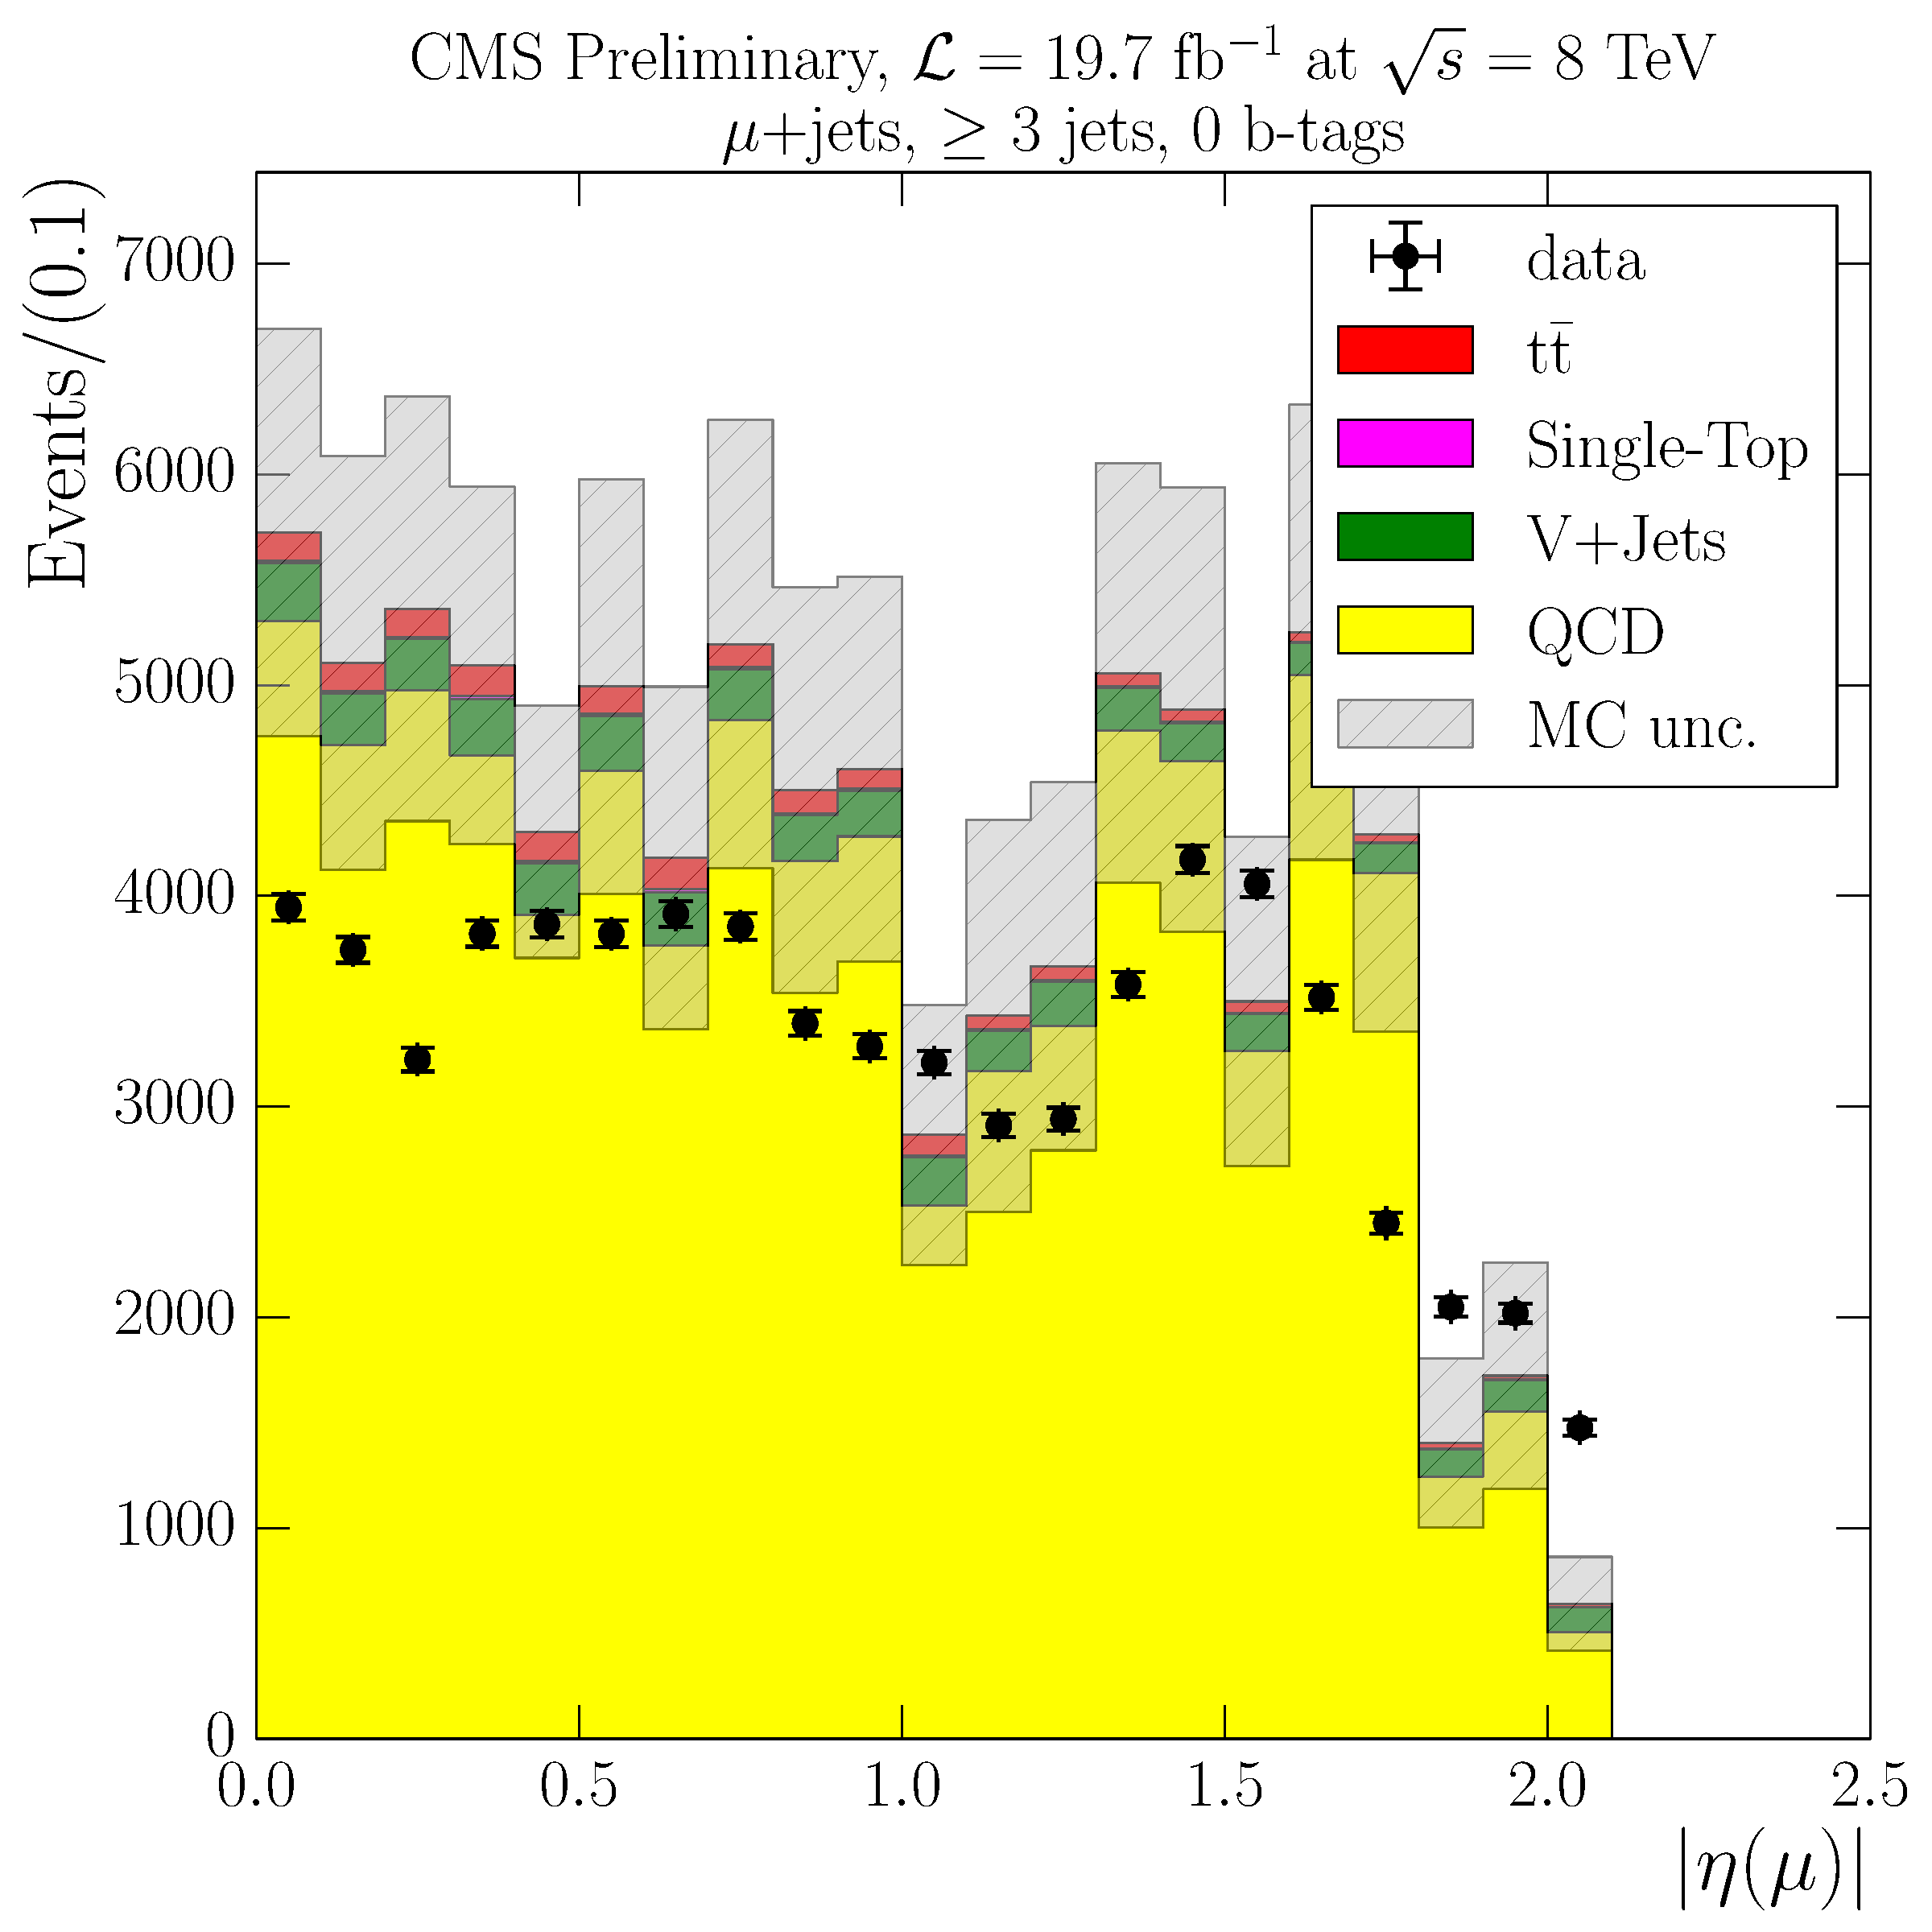
\includegraphics[width=0.47\textwidth]{QCD/QCD_non_iso_control_region_muon_AbsEta_0btag}}
    \caption[Muon relative isolation with no isolation cut and muon $\abs \eta$ for non-isolated selection in muon plus
    jets events]{Muon relative isolation with no isolation cut (a) and muon $\abs \eta$ (b) for non-isolated ($\reliso >
    0.3$) selection in muon plus jets events with at least three jets and 0 b-tagged jets. The vertical red line on plot
    (a) shows the \reliso cut value of \num{0.3}.}
    \label{fig:qcd_muon_plots}
\end{figure}

\section{Data/MC comparison}
\label{s_xsection:data_mc_comparison}
%explain the MC error on the plots. explain the yields.

In this section, the agreement between simulation and data for various kinematic distributions is reviewed after the
final event selection. The event yields for all selection steps described in Section~\ref{s_xsection:event_selection}
are shown in Tables~\ref{tab:event_yields_ejets} and \ref{tab:event_yields_mujets} for the electron and muon channels,
respectively. All background events are normalised to the number of expected events for the total integrated luminosity
of \SI{19.7}{\fbinv}.

The QCD multi-jet background events shown in plots are derived using the data-driven methods explained previously.
Figure~\ref{fig:contol_plots_leptons} shows the lepton \pt and $\abs \eta$ distributions for both electrons and muons.
In Figure~\ref{fig:contol_plots_METs}, missing transverse energy distributions are shown, also including the
logarithmic scale for higher values of \MET. Figure~\ref{fig:contol_plots_phiMET_NJets} shows the azimuthal angle of
\MET ($\phi(\MET)$) and jet multiplicity distributions for both channels. The \ttbar uncertainty shown in the plots
refers to the theoretical uncertainty on the NNLO calculation of the total \ttbar cross section at \SI{8}{\TeV}
\autocite{NNLO_ttbar} used in this analysis.

Overall, good agreement is found between data and Monte Carlo simulation in all kinematic distributions. One should note
that the comparison shown is made before the fitting process, which is described in
Section~\ref{s_xsection:measurement}.

\begin{table}
  \centering
   \caption[Number of expected and observed events from simulation and data in the electron channel]{Number of expected
   and observed events from simulation and data in the electron channel out of the box, i.e.\ before the fitting
   process.}
    \label{tab:event_yields_ejets}
    \resizebox{\columnwidth}{!} {
    \begin{tabular}{lrrrrrrr}
    \toprule
	\textbf{Selection step} & \textbf{\ttjets} & \textbf{\WpJets} & \textbf{\ZpJets} & \textbf{Single top} & \textbf{QCD} & \textbf{Sum MC} & \textbf{Data} \\
	\midrule
	Preselection  &  $1346476 \pm 1028$ &  $1727900 \pm 1138$ &  $380944 \pm 234$ &  $169689 \pm 262$ &  $130308513 \pm 475118$ &  $133933524 \pm 475120$ &  13042702 \\ 
	Event cleaning/HLT  &  $385009 \pm 553$ &  $516544 \pm 600$ &  $147515 \pm 143$ &  $37308 \pm 127$ &  $3854386 \pm 83441$ &  $4940764 \pm 83445$ &  5846672 \\ 
	One isolated electron  &  $342394 \pm 522$ &  $446691 \pm 548$ &  $100243 \pm 117$ &  $33000 \pm 120$ &  $578895 \pm 29802$ &  $1501225 \pm 29812$ &  1688811 \\ 
	Muon veto  &  $323759 \pm 508$ &  $446579 \pm 548$ &  $99805 \pm 117$ &  $32301 \pm 118$ &  $578860 \pm 29802$ &  $1481306 \pm 29812$ &  1668851 \\ 
	Dilepton veto  &  $319019 \pm 504$ &  $446469 \pm 548$ &  $73876 \pm 101$ &  $32117 \pm 118$ &  $578821 \pm 29802$ &  $1450305 \pm 29812$ &  1628009 \\ 
	Conversion veto  &  $310863 \pm 498$ &  $430191 \pm 538$ &  $70929 \pm 99$ &  $31287 \pm 116$ &  $321292 \pm 21826$ &  $1164563 \pm 21839$ &  1396638 \\ 
	$\geq 1$ jets  &  $310863 \pm 498$ &  $430179 \pm 538$ &  $70928 \pm 99$ &  $31287 \pm 116$ &  $321292 \pm 21826$ &  $1164550 \pm 21839$ &  1396638 \\ 
	$\geq 2$ jets  &  $310838 \pm 498$ &  $429195 \pm 536$ &  $70723 \pm 99$ &  $31279 \pm 116$ &  $320506 \pm 21819$ &  $1162543 \pm 21831$ &  1396506 \\ 
	$\geq 3$ jets  &  $306406 \pm 494$ &  $386892 \pm 493$ &  $63653 \pm 90$ &  $29953 \pm 114$ &  $226938 \pm 16321$ &  $1013843 \pm 16337$ &  1215535 \\ 
	$\geq 4$ jets  &  $174701 \pm 373$ &  $76646 \pm 179$ &  $13323 \pm 35$ &  $9765 \pm 67$ &  $44203 \pm 4340$ &  $318640 \pm 4361$ &  351194 \\ 
	$\geq 1$ b-tagged jets  &  $148287 \pm 341$ &  $11280 \pm 69$ &  $2152 \pm 14$ &  $7675 \pm 58$ &  $9304 \pm 2055$ &  $178700 \pm 2085$ &  182481 \\ 
	$\geq 2$ b-tagged jets  &  $70103 \pm 228$ &  $1320 \pm 23$ &  $337 \pm 5$ &  $2900 \pm 35$ &  $3035 \pm 1789$ &  $77697 \pm 1804$ &  76379 \\ 
	\bottomrule
	\end{tabular}
	}
\end{table}

\begin{table}
  \centering
   \caption[Number of expected and observed events from simulation and data in the muon channel]{Number of expected and
   observed events from simulation and data in the muon channel out of the box, i.e.\ before the fitting process.}
    \label{tab:event_yields_mujets}
    \resizebox{\columnwidth}{!} {
    \begin{tabular}{lrrrrrrr}
    \toprule
	\textbf{Selection step} & \textbf{\ttjets} & \textbf{\WpJets} & \textbf{\ZpJets} & \textbf{Single top} & \textbf{QCD} & \textbf{Sum MC} & \textbf{Data} \\
	\midrule
	Preselection  &  $1346476 \pm 1028$ &  $1727900 \pm 1138$ &  $380944 \pm 234$ &  $169689 \pm 262$ &  $104079124 \pm 236784$ &  $107704135 \pm 236789$ &  20284215 \\ 
	Event cleaning/HLT  &  $443056 \pm 581$ &  $644505 \pm 688$ &  $148143 \pm 142$ &  $44727 \pm 135$ &  $1664036 \pm 33747$ &  $2944468 \pm 33759$ &  3063569 \\ 
	One isolated muon  &  $360897 \pm 521$ &  $473825 \pm 556$ &  $88283 \pm 106$ &  $35546 \pm 121$ &  $83535 \pm 5833$ &  $1042088 \pm 5885$ &  1327738 \\ 
	Second muon veto  &  $353646 \pm 516$ &  $473776 \pm 556$ &  $53263 \pm 82$ &  $35260 \pm 120$ &  $82863 \pm 5823$ &  $998811 \pm 5874$ &  1254896 \\ 
	Electron veto  &  $336474 \pm 503$ &  $473631 \pm 556$ &  $52935 \pm 82$ &  $34633 \pm 119$ &  $82841 \pm 5823$ &  $980516 \pm 5873$ &  1237495 \\ 
	$\geq 1$ jets  &  $336474 \pm 503$ &  $473622 \pm 556$ &  $52934 \pm 82$ &  $34633 \pm 119$ &  $82841 \pm 5823$ &  $980507 \pm 5873$ &  1237495 \\ 
	$\geq 2$ jets  &  $336457 \pm 503$ &  $472377 \pm 554$ &  $52768 \pm 81$ &  $34620 \pm 119$ &  $81211 \pm 5777$ &  $977436 \pm 5827$ &  1237428 \\ 
	$\geq 3$ jets  &  $332863 \pm 501$ &  $425334 \pm 507$ &  $47493 \pm 74$ &  $33146 \pm 117$ &  $33505 \pm 2726$ &  $872343 \pm 2822$ &  1108272 \\ 
	$\geq 4$ jets  &  $188466 \pm 377$ &  $83248 \pm 184$ &  $10144 \pm 29$ &  $10556 \pm 67$ &  $7006 \pm 1155$ &  $299422 \pm 1231$ &  340786 \\ 
	$\geq 1$ b-tagged jets  &  $160223 \pm 344$ &  $12341 \pm 71$ &  $1690 \pm 12$ &  $8322 \pm 59$ &  $3763 \pm 910$ &  $186341 \pm 977$ &  196667 \\ 
	$\geq 2$ b-tagged jets  &  $76068 \pm 231$ &  $1465 \pm 24$ &  $248 \pm 4$ &  $3096 \pm 35$ &  $481 \pm 413$ &  $81361 \pm 476$ &  85028 \\ 
	\bottomrule
	\end{tabular}
	}
\end{table}



\begin{figure}[htbp]
	\centering
  	\subfloat[]{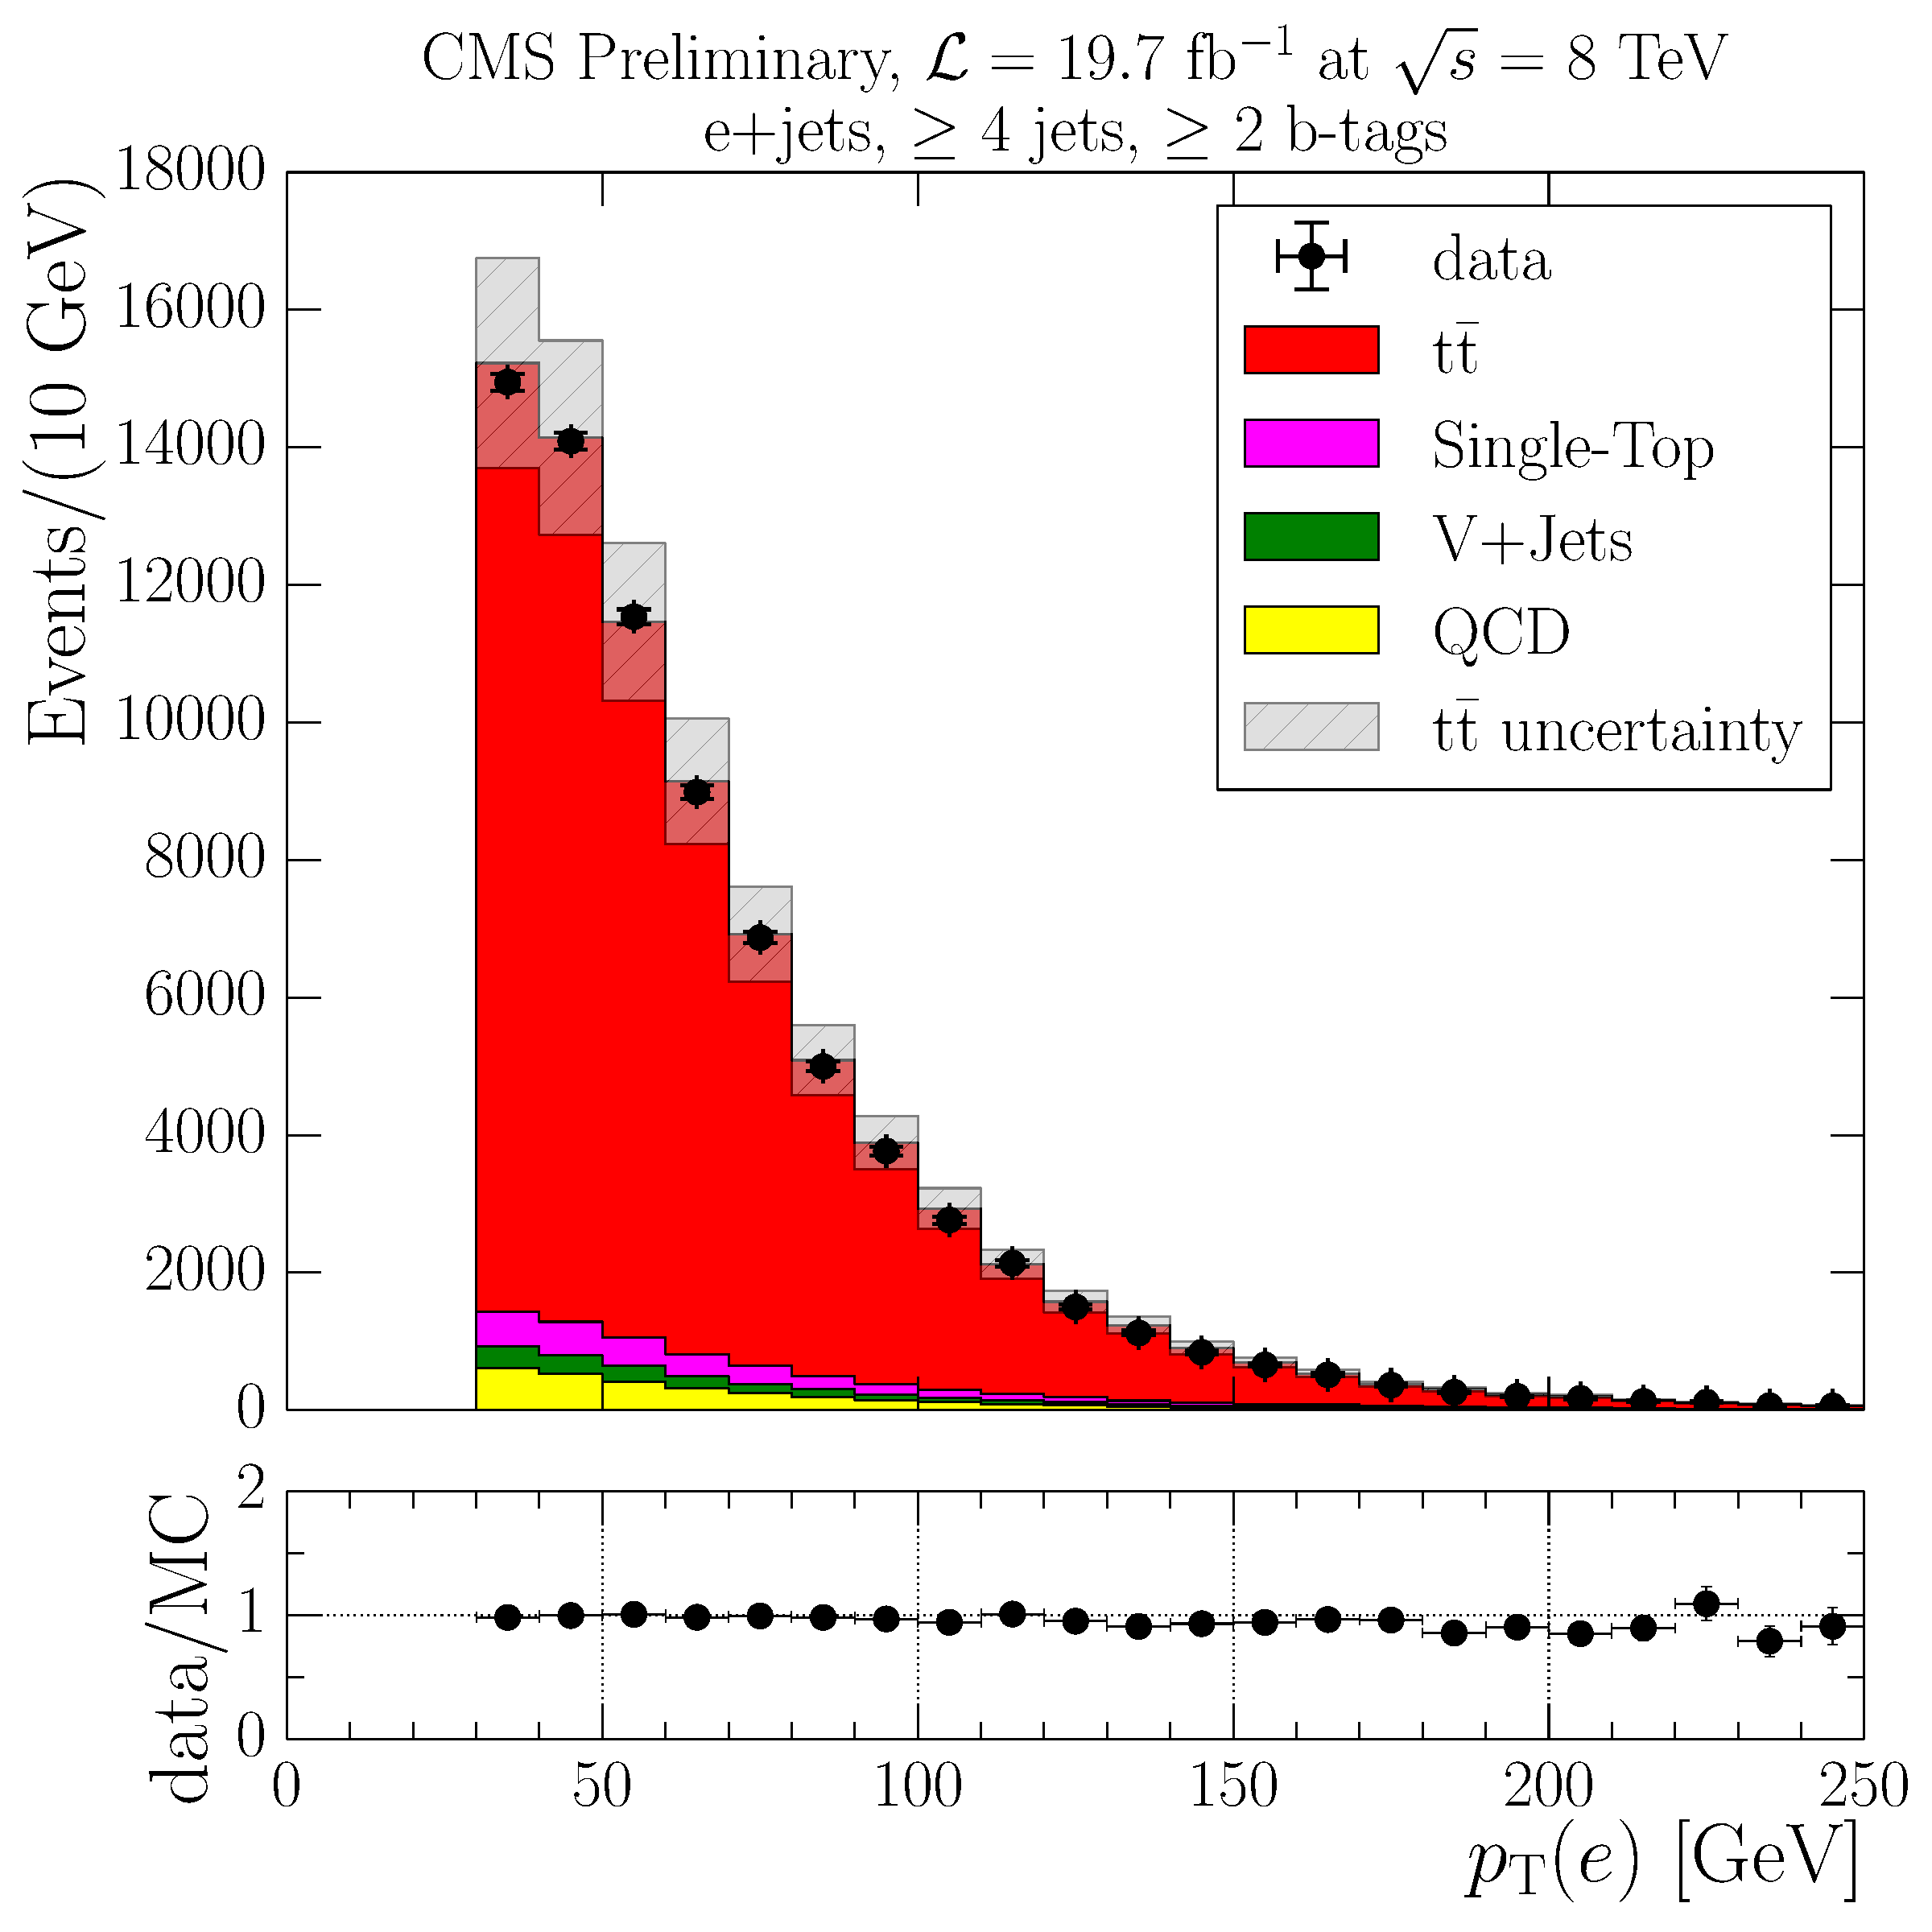
\includegraphics[width=0.50\textwidth]{control_plots/electron_pT_2orMoreBtags_with_ratio}}\hfill
  	\subfloat[]{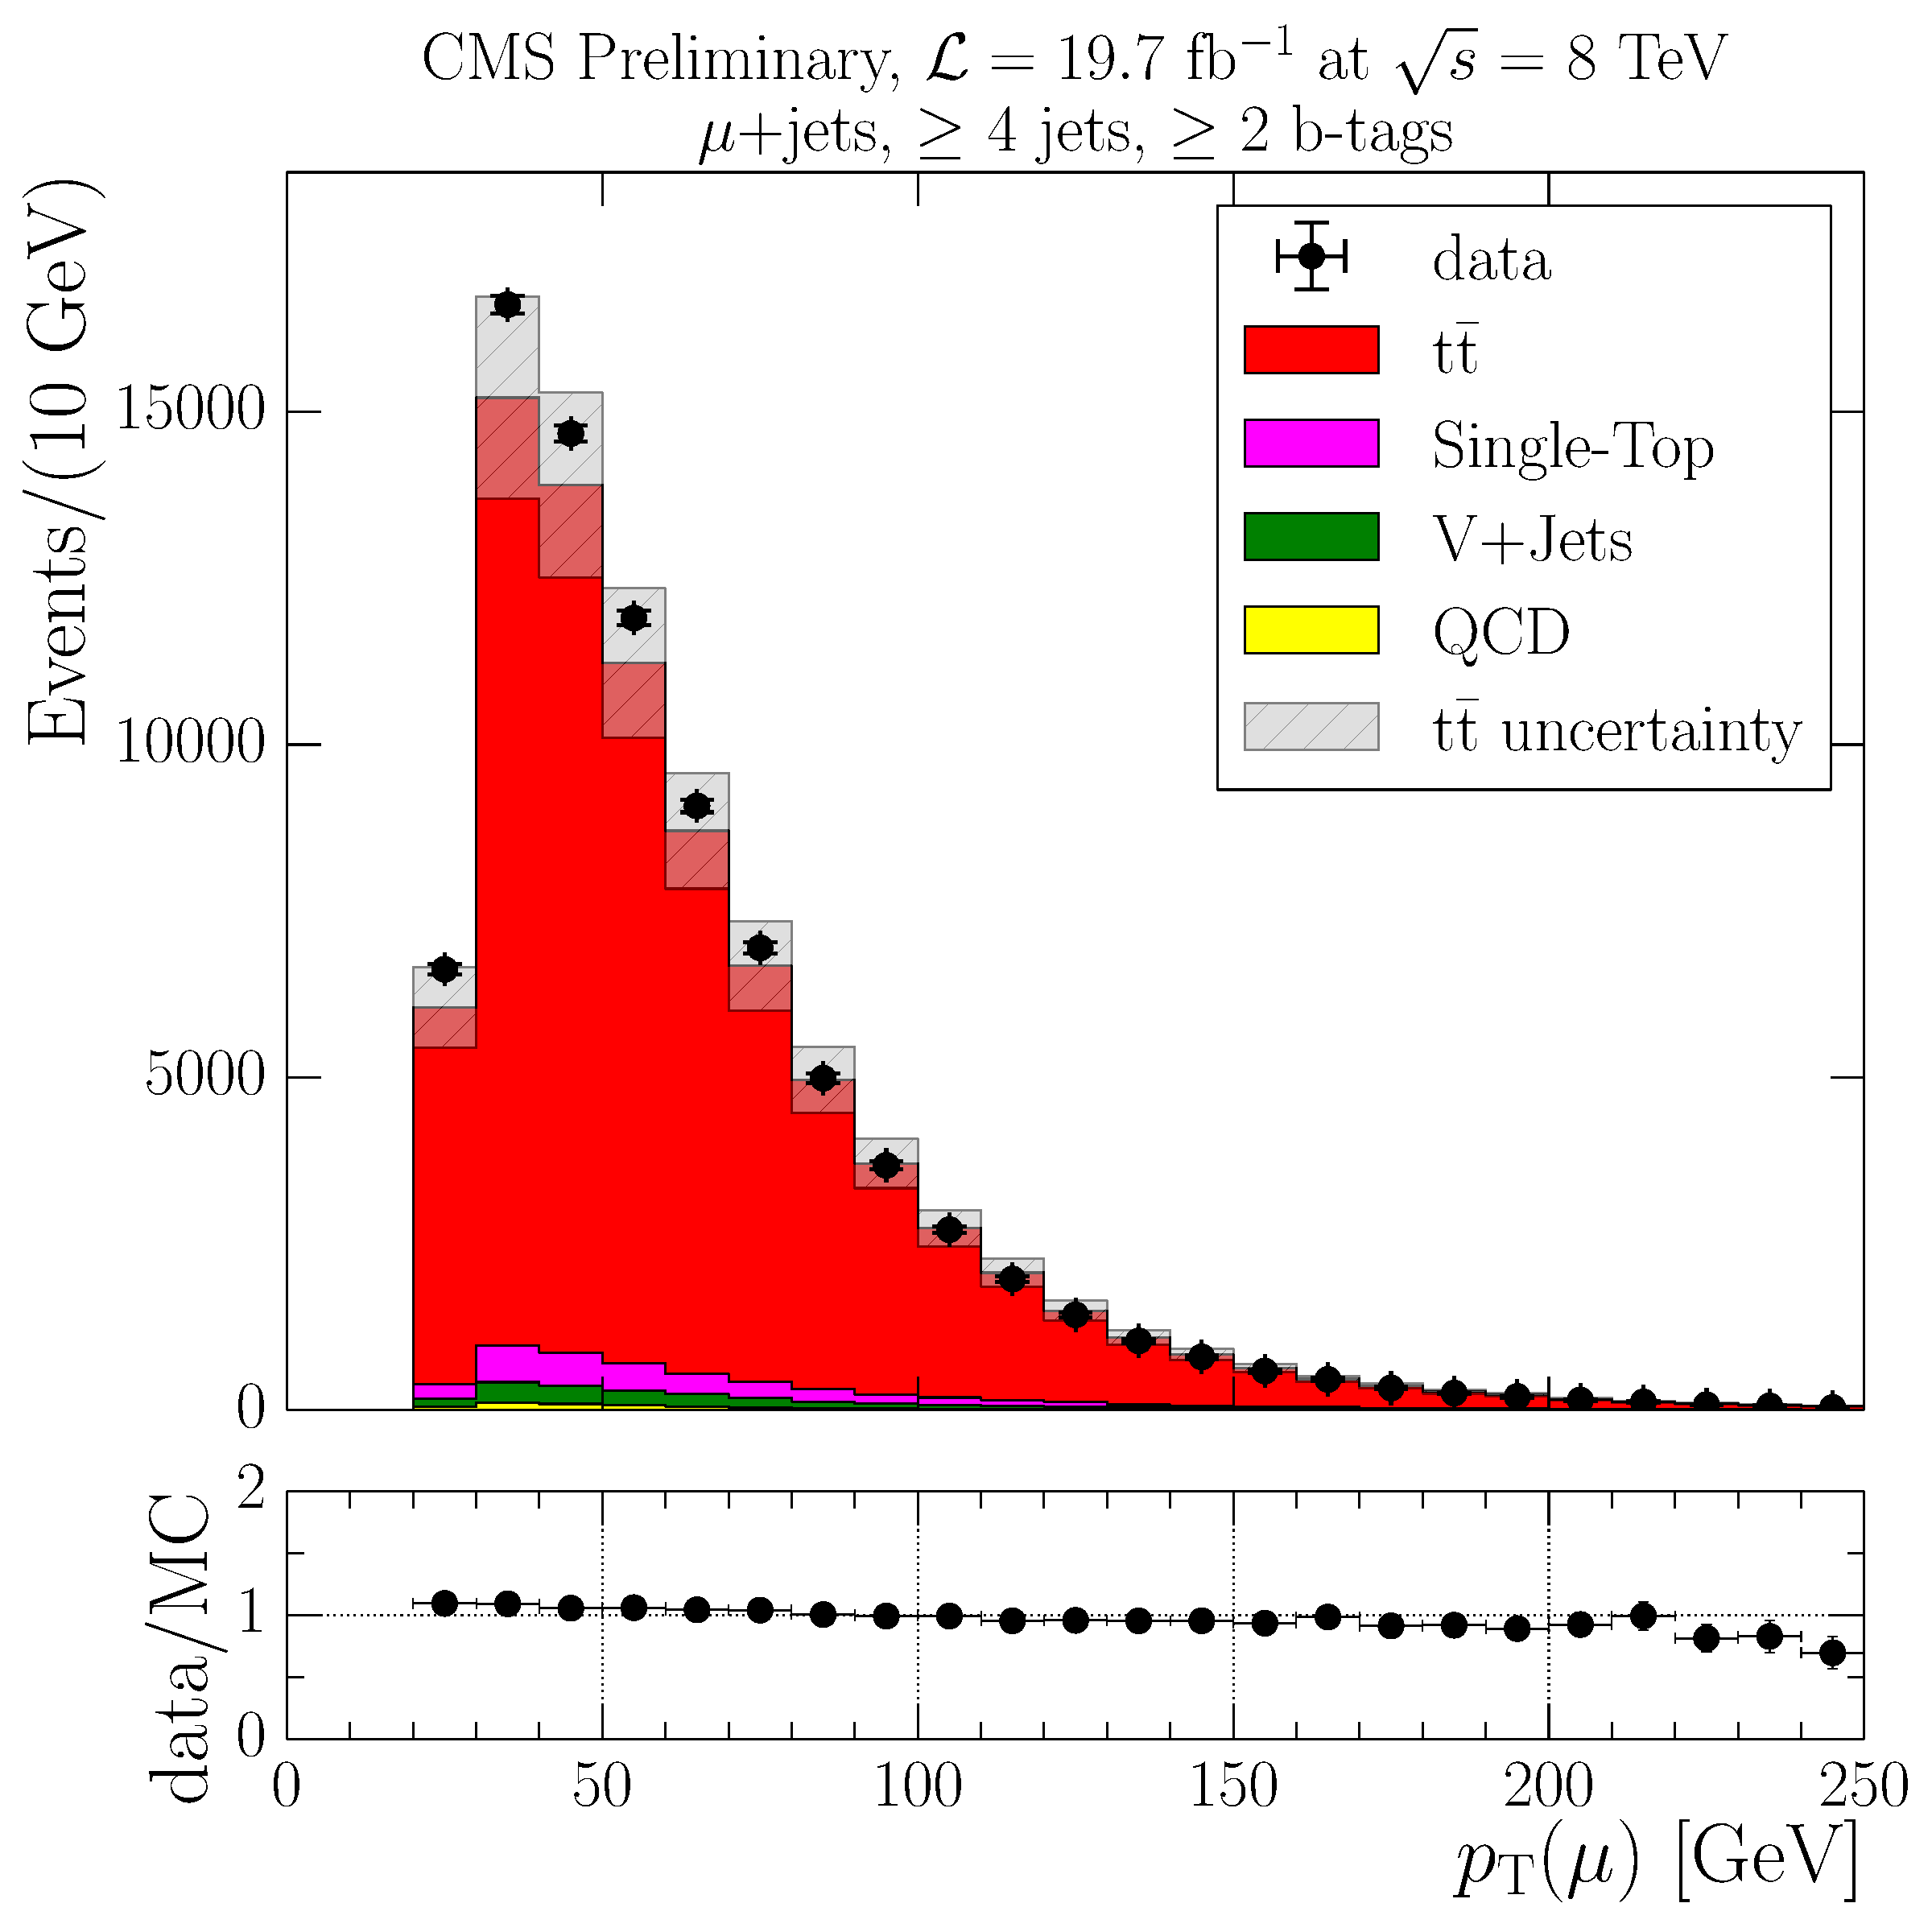
\includegraphics[width=0.50\textwidth]{control_plots/muon_pT_2orMoreBtags_with_ratio}} \\
  	\subfloat[]{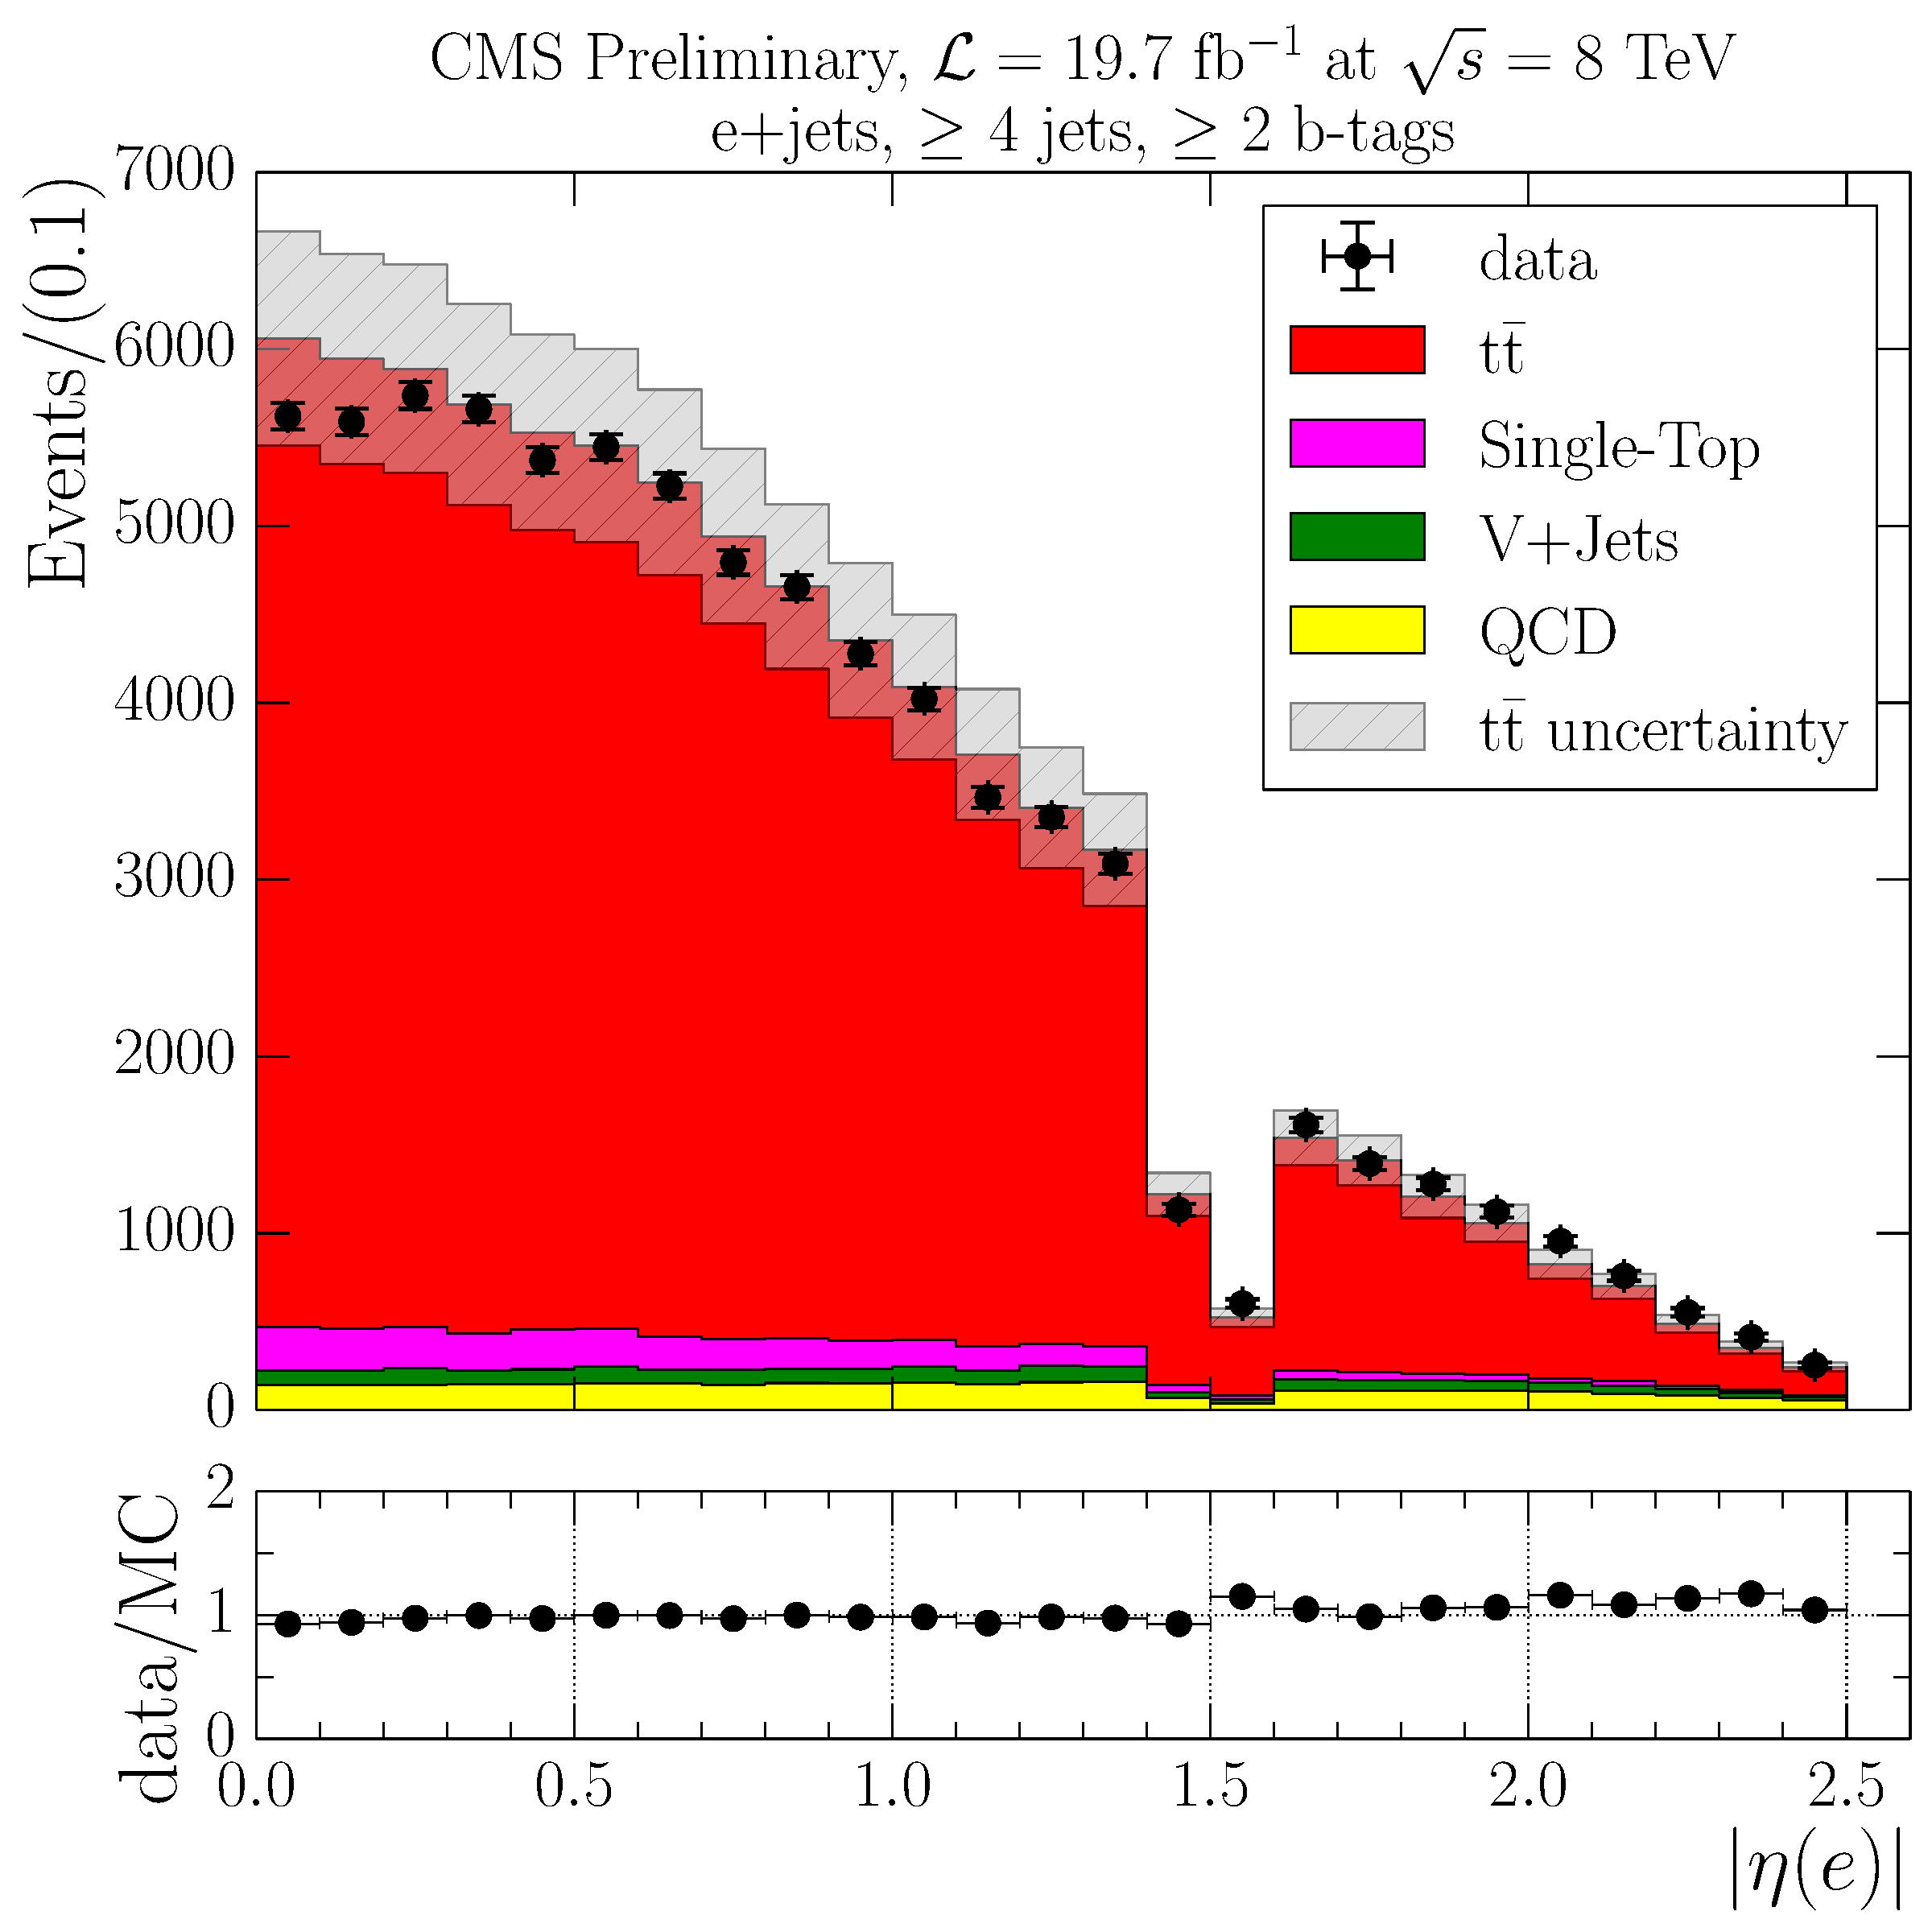
\includegraphics[width=0.50\textwidth]{control_plots/electron_AbsEta_2orMoreBtags_with_ratio}}\hfill
  	\subfloat[]{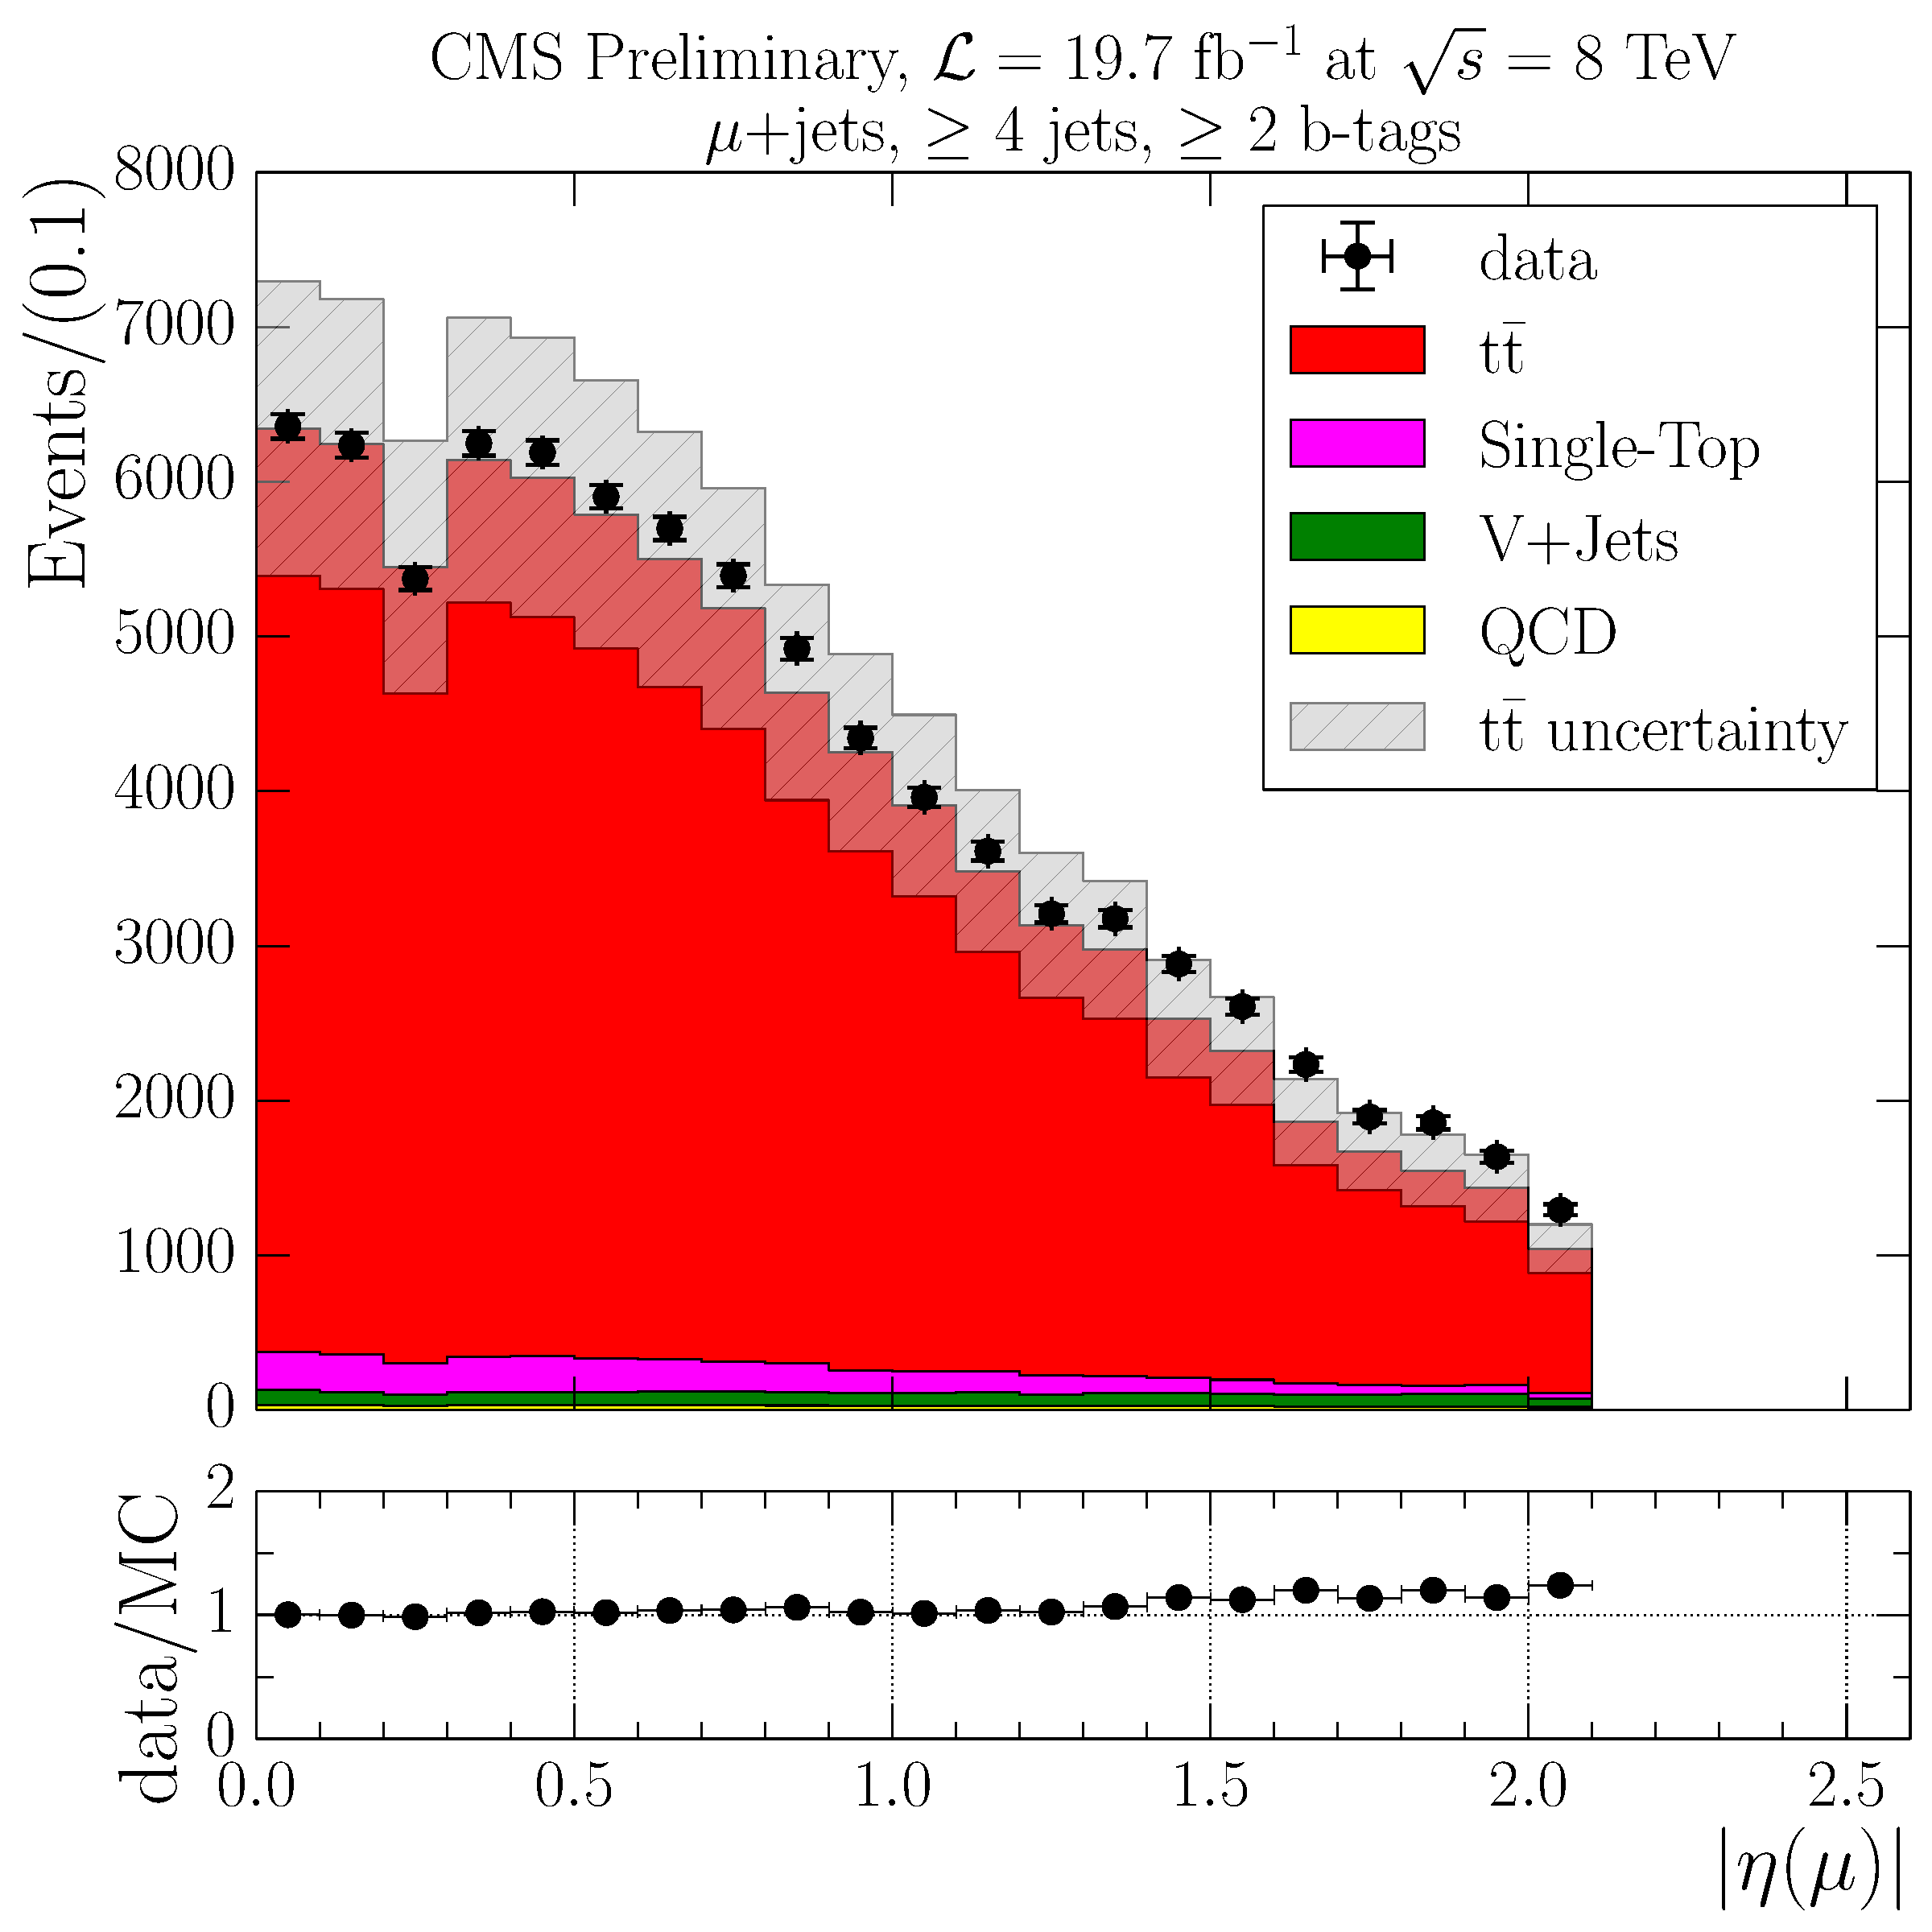
\includegraphics[width=0.50\textwidth]{control_plots/muon_AbsEta_2orMoreBtags_with_ratio}}
    \caption[Data/MC comparison plots of electron and muon \pt and $\abs \eta$ after the final event selection]{Data/MC
    comparison plots after the final event selection: electron \pt (a), muon \pt (b), electron $\abs \eta$ (c) and muon
    $\abs \eta$ (d). Left-hand plots: electron plus jets selection, right-hand plots: muon plus jets selection.}
    \label{fig:contol_plots_leptons}
\end{figure}

\begin{figure}[htbp]
	\centering
  	\subfloat[]{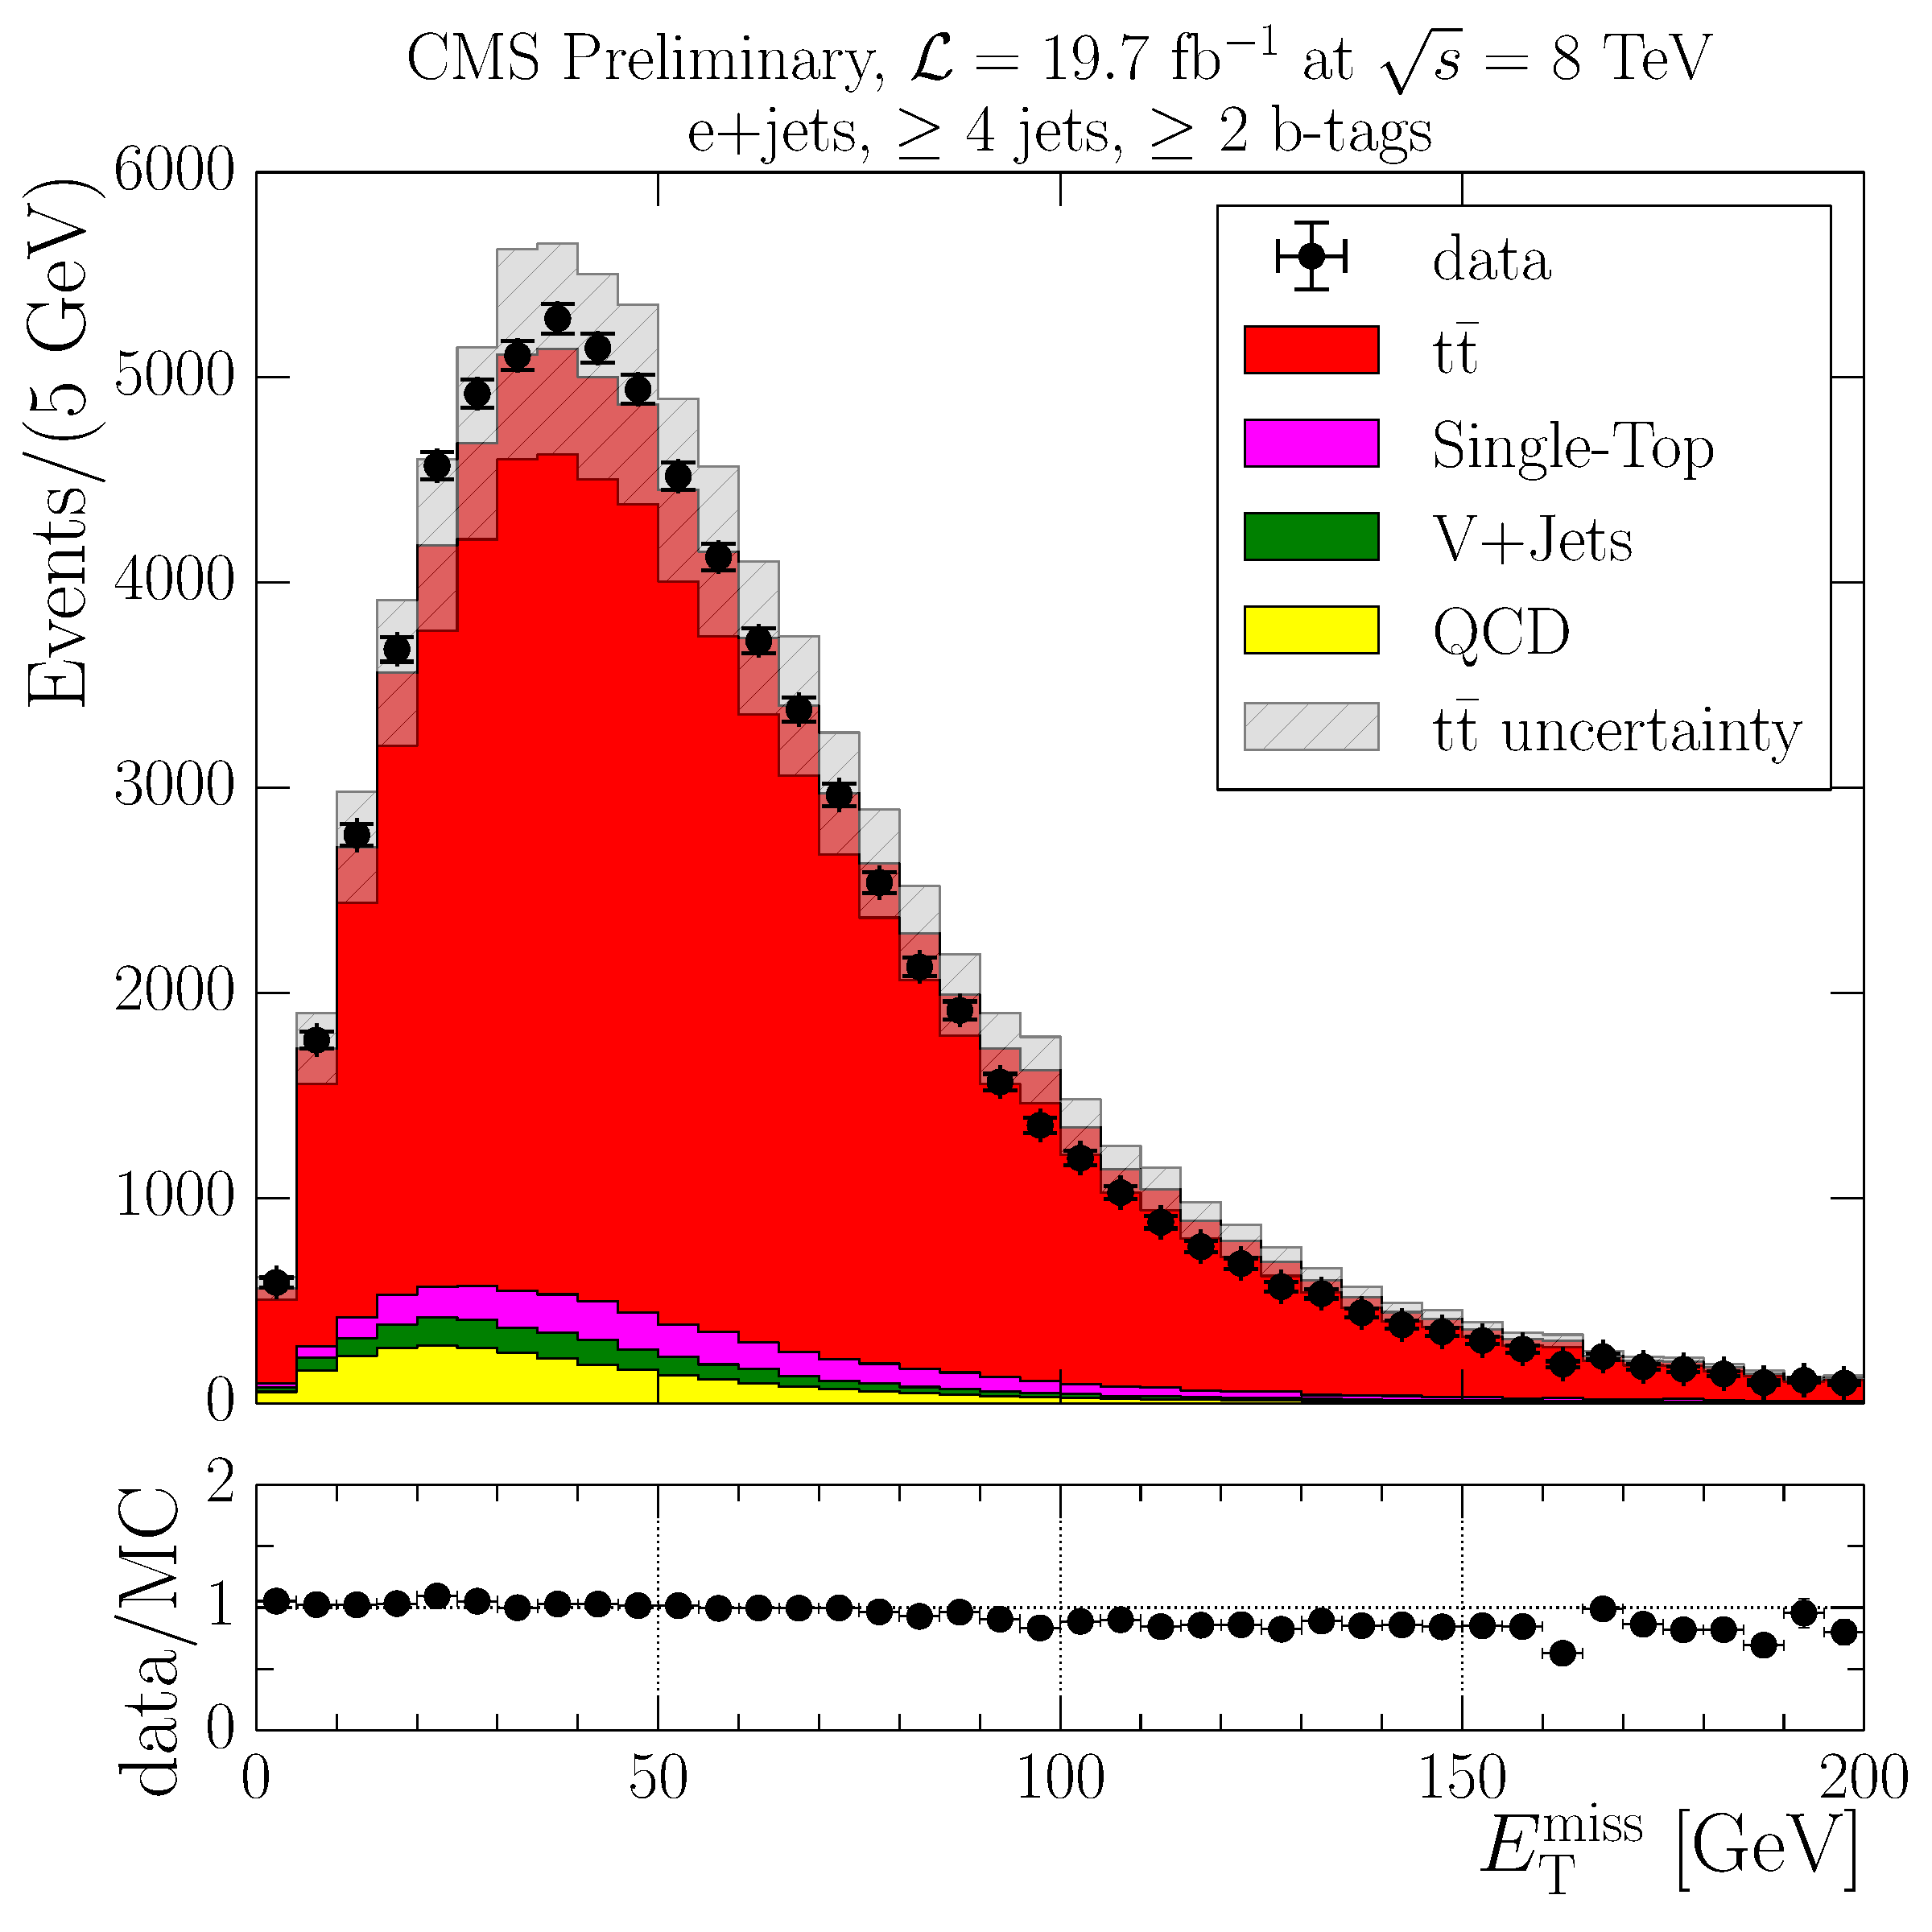
\includegraphics[width=0.50\textwidth]{control_plots/EPlusJets_patType1CorrectedPFMet_2orMoreBtags_with_ratio}}\hfill
  	\subfloat[]{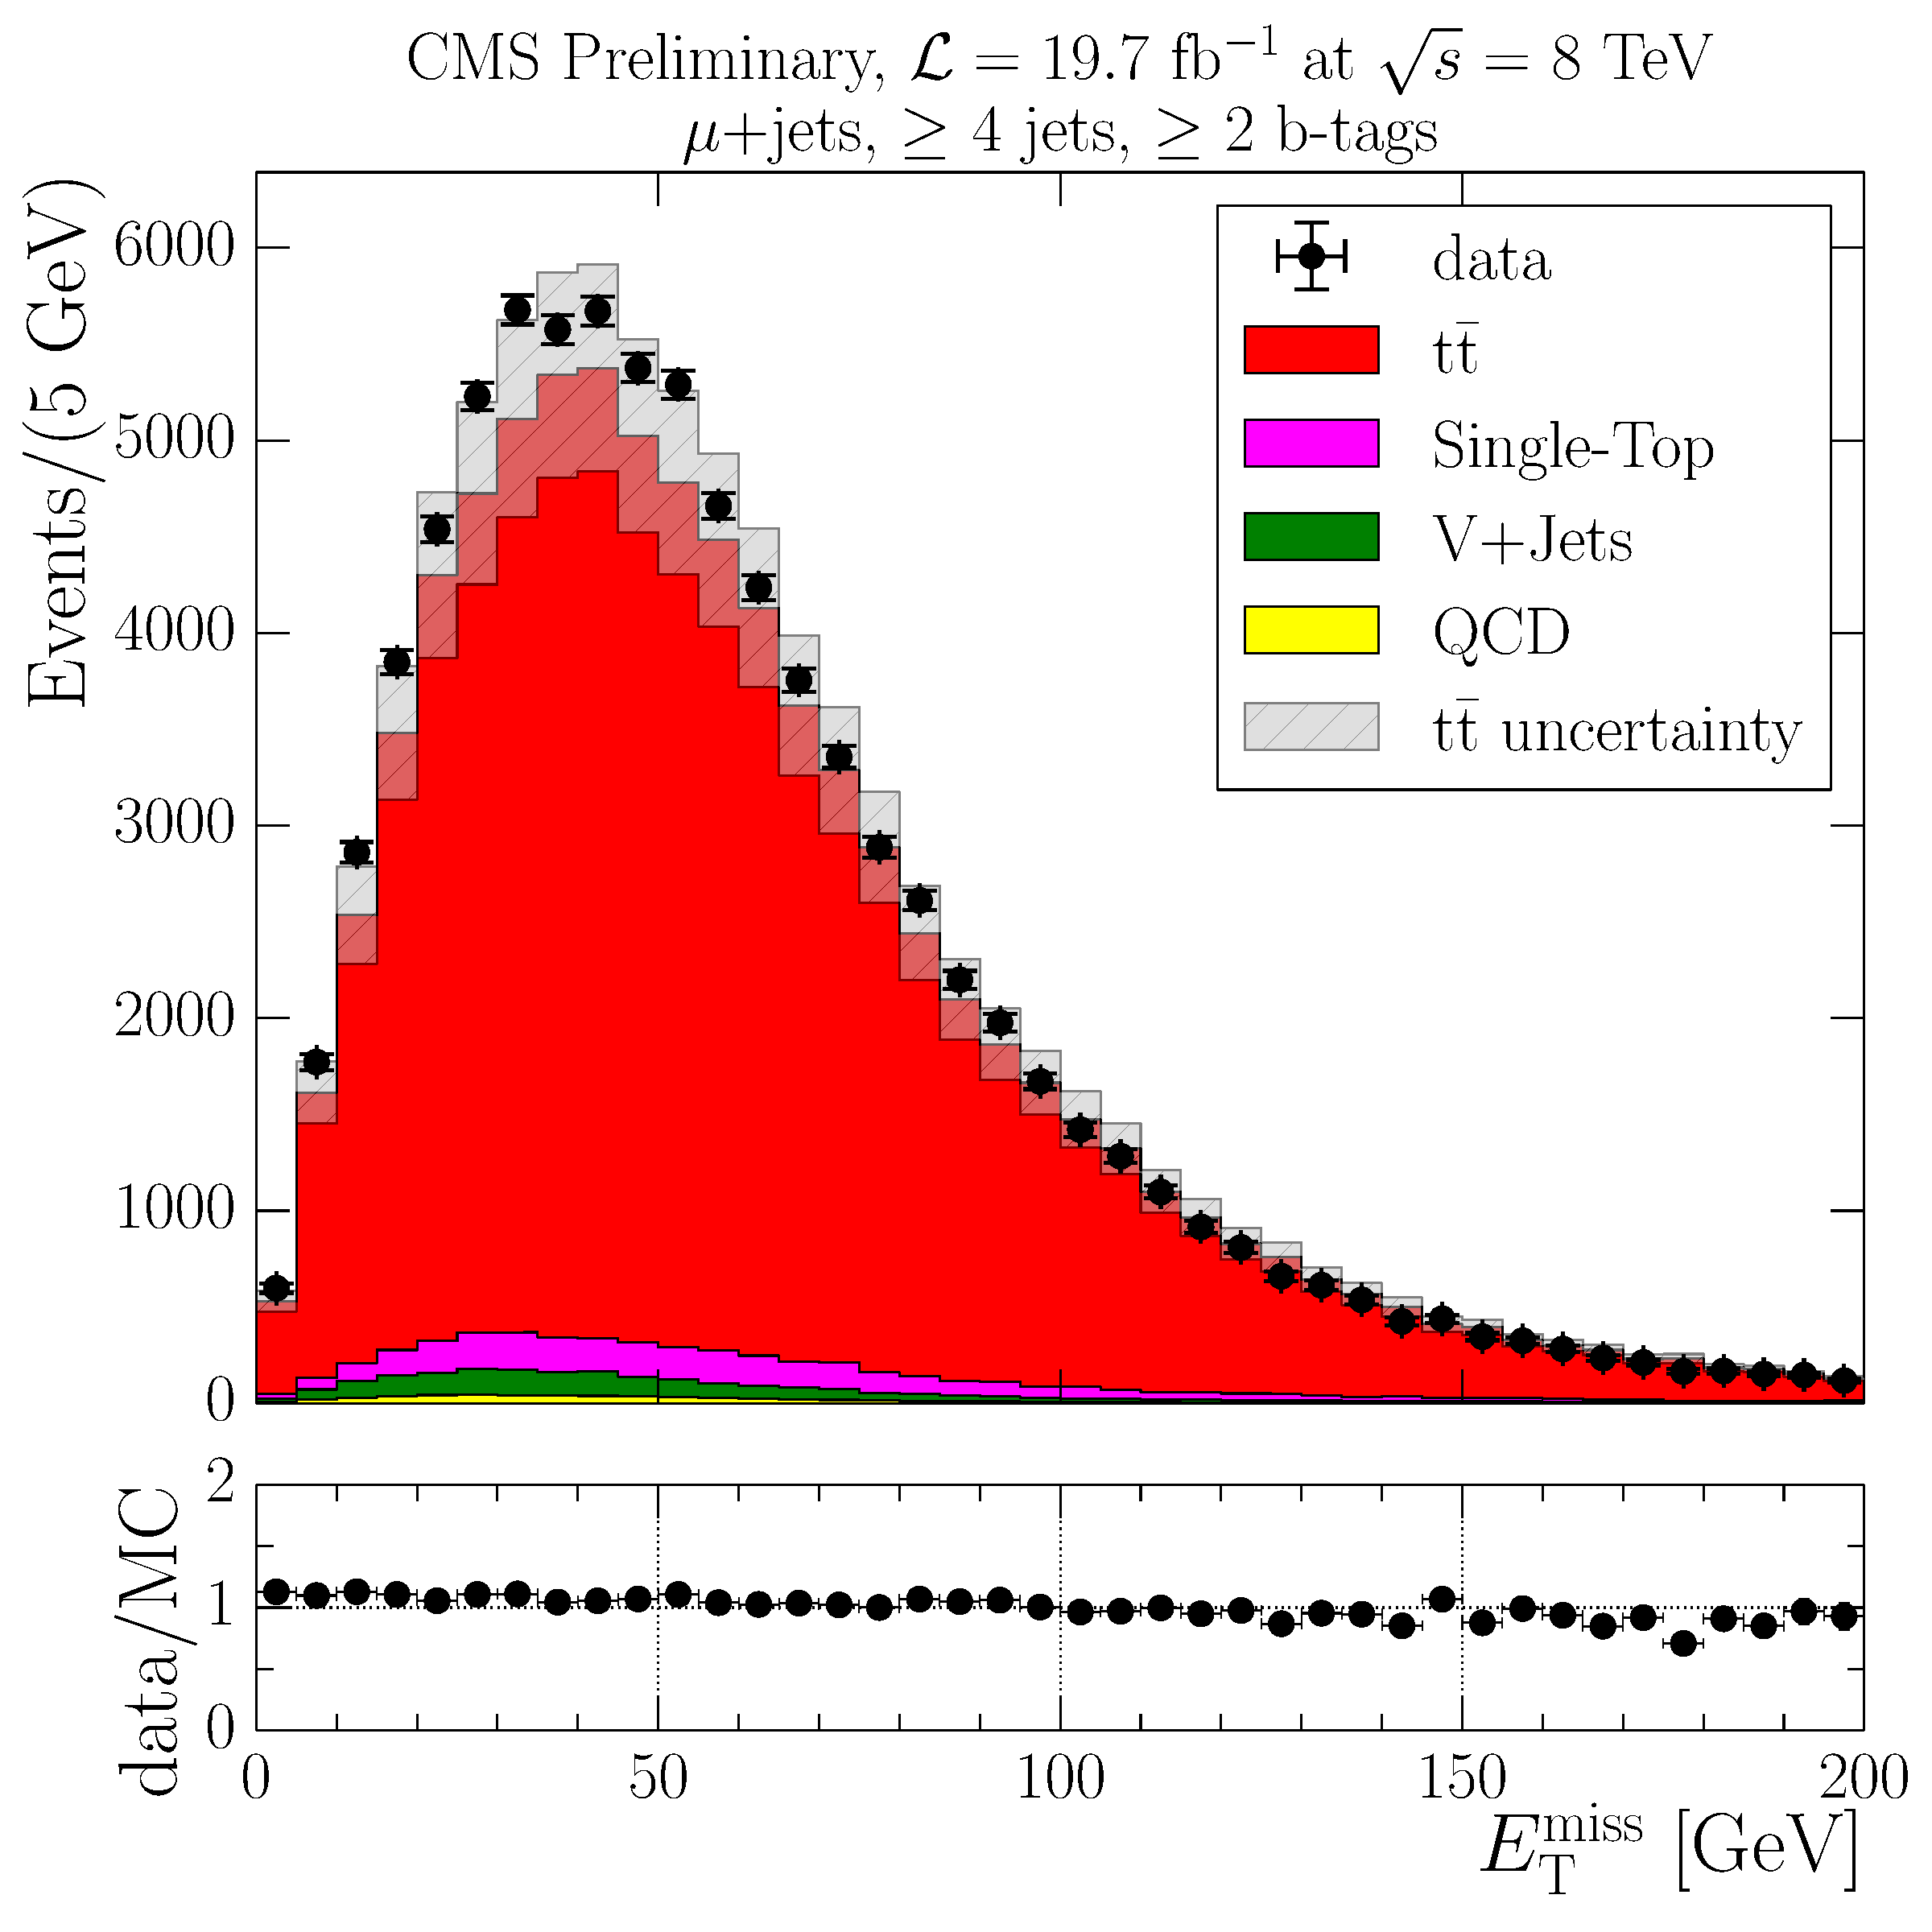
\includegraphics[width=0.50\textwidth]{control_plots/MuPlusJets_patType1CorrectedPFMet_2orMoreBtags_with_ratio}} \\
  	\subfloat[]{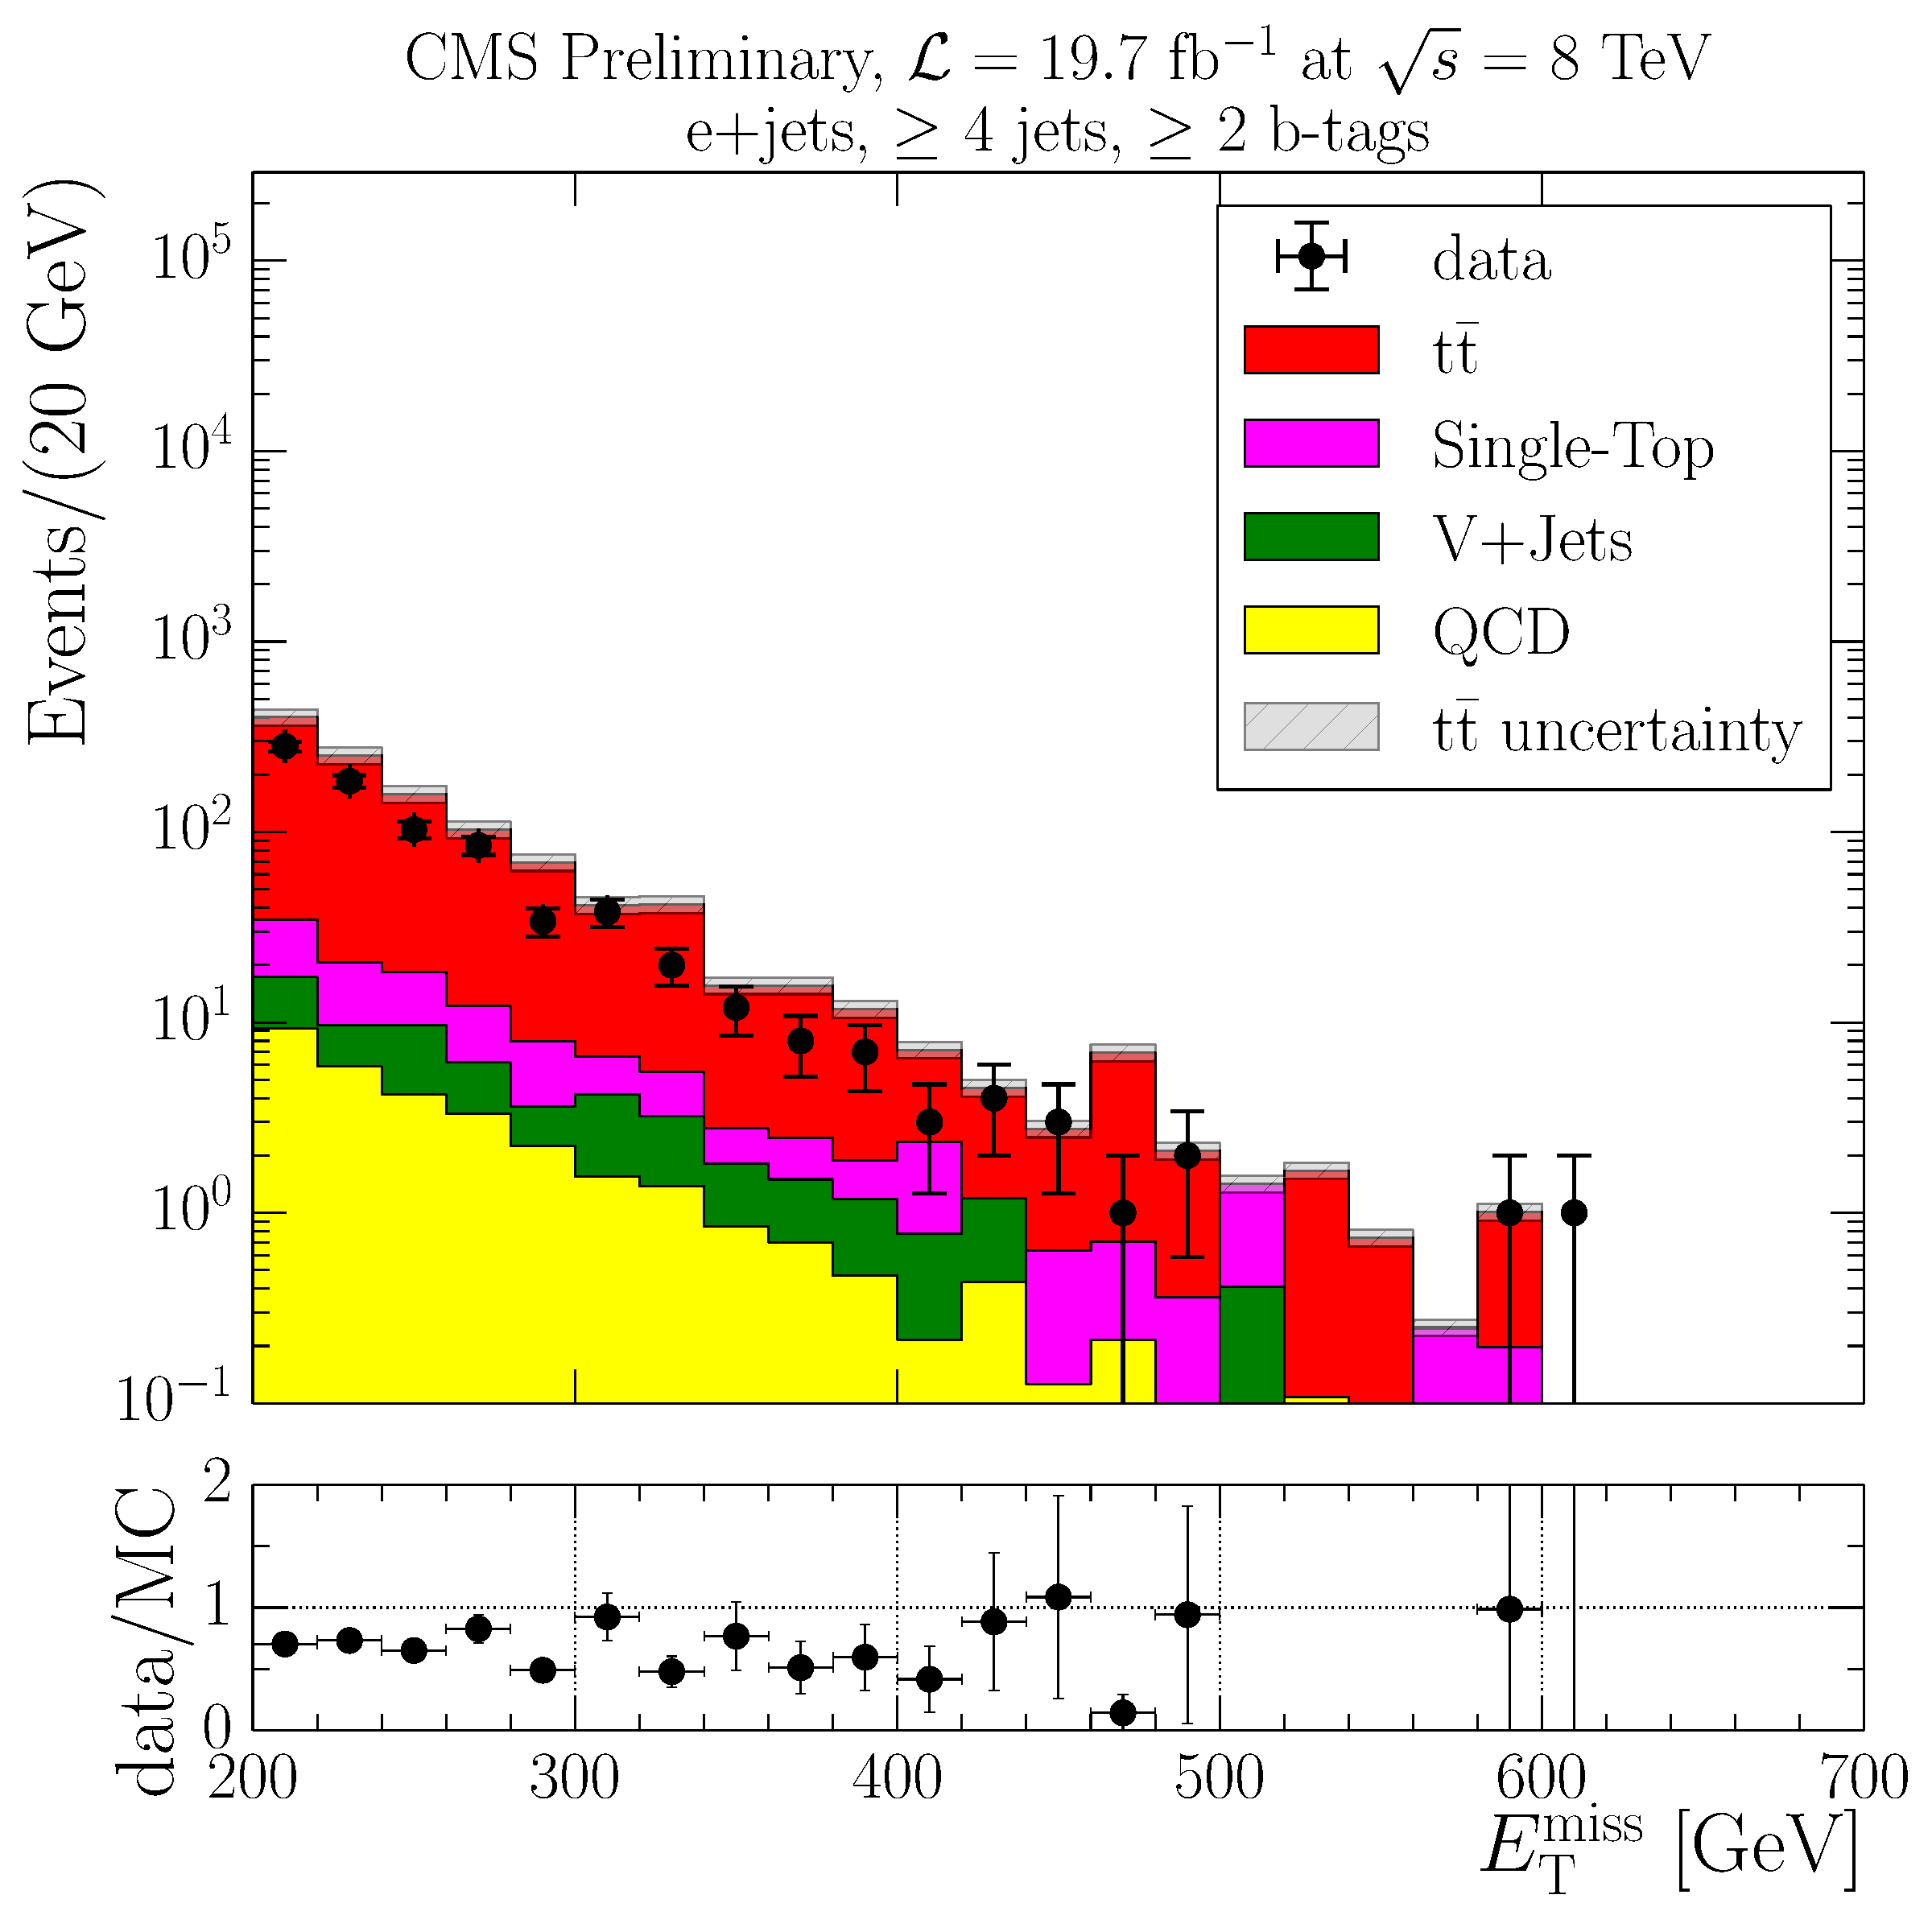
\includegraphics[width=0.50\textwidth]{control_plots/EPlusJets_patType1CorrectedPFMet_log_2orMoreBtags_with_ratio}}\hfill
  	\subfloat[]{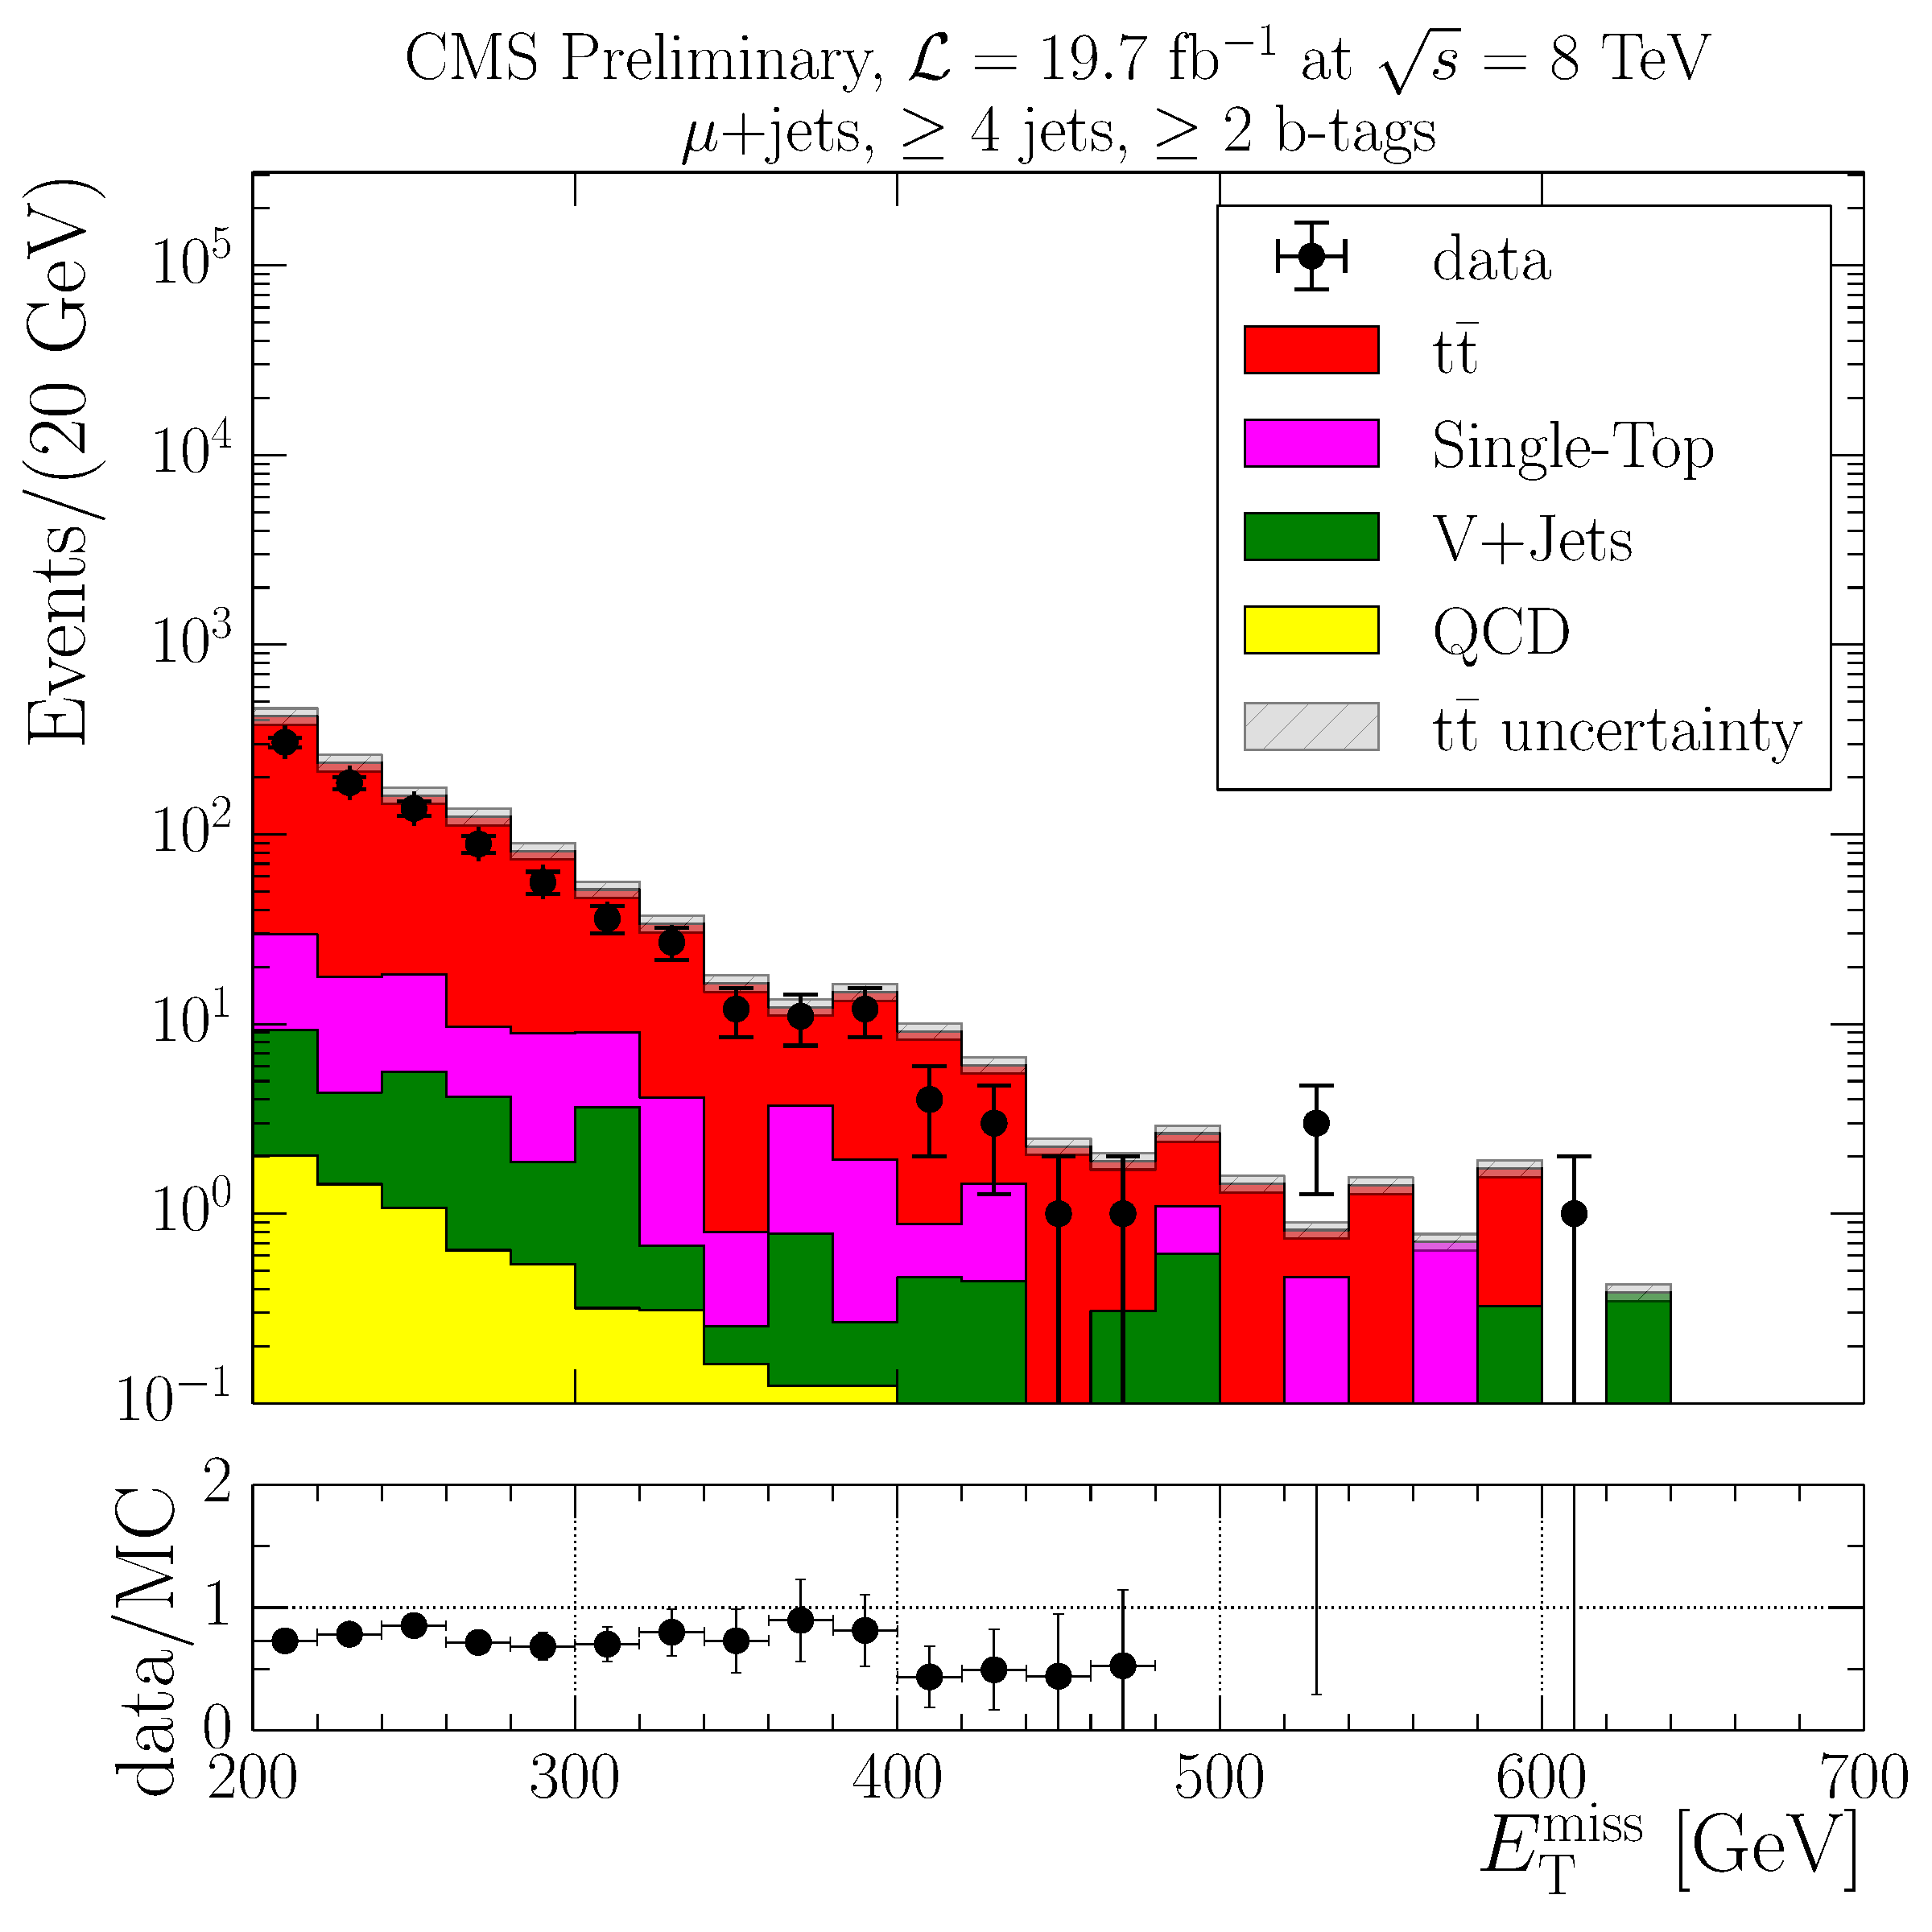
\includegraphics[width=0.50\textwidth]{control_plots/MuPlusJets_patType1CorrectedPFMet_log_2orMoreBtags_with_ratio}} \\
    \caption[Data/MC comparison plots of \MET after the final event selection]{Data/MC comparison plots of \MET (a, b)
    and logarithmic view of \MET (c, d) after the final event selection. Left-hand plots: electron plus jets selection,
    right-hand plots: muon plus jets selection.}
    \label{fig:contol_plots_METs}
\end{figure}

\begin{figure}[htbp]
	\centering
  	\subfloat[]{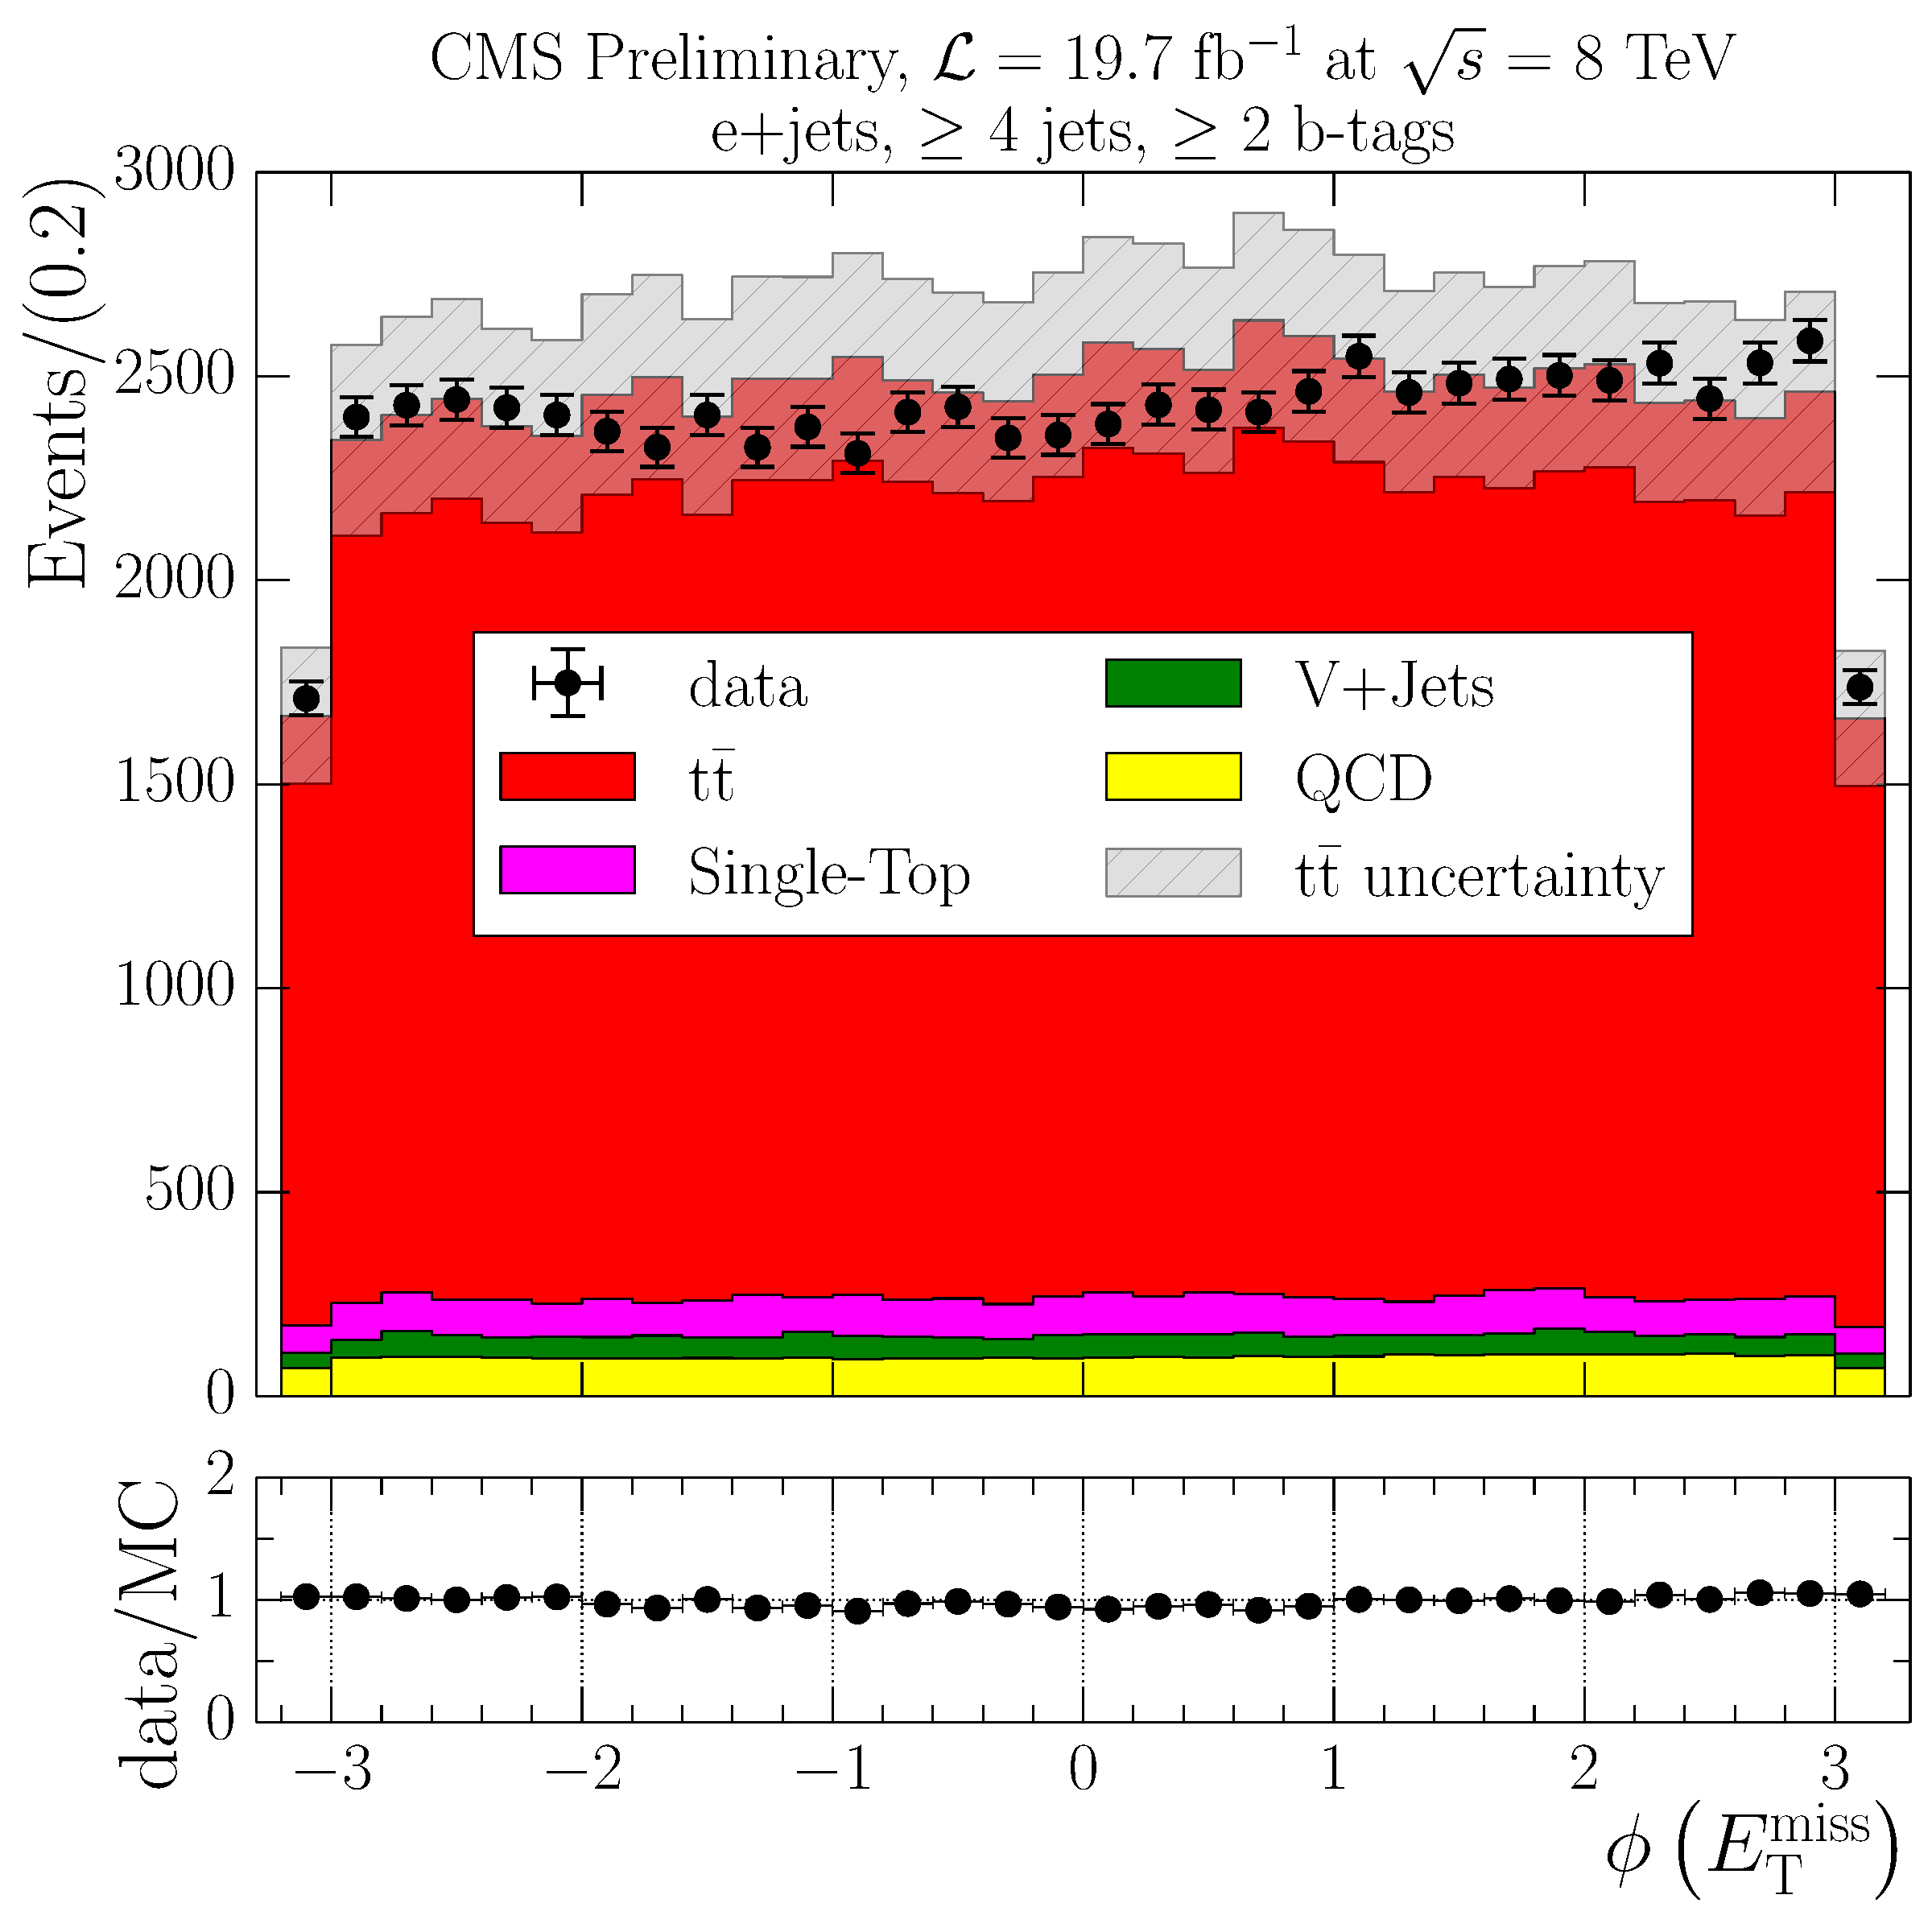
\includegraphics[width=0.50\textwidth]{control_plots/EPlusJets_patType1CorrectedPFMet_phi_2orMoreBtags_with_ratio}}\hfill
	\subfloat[]{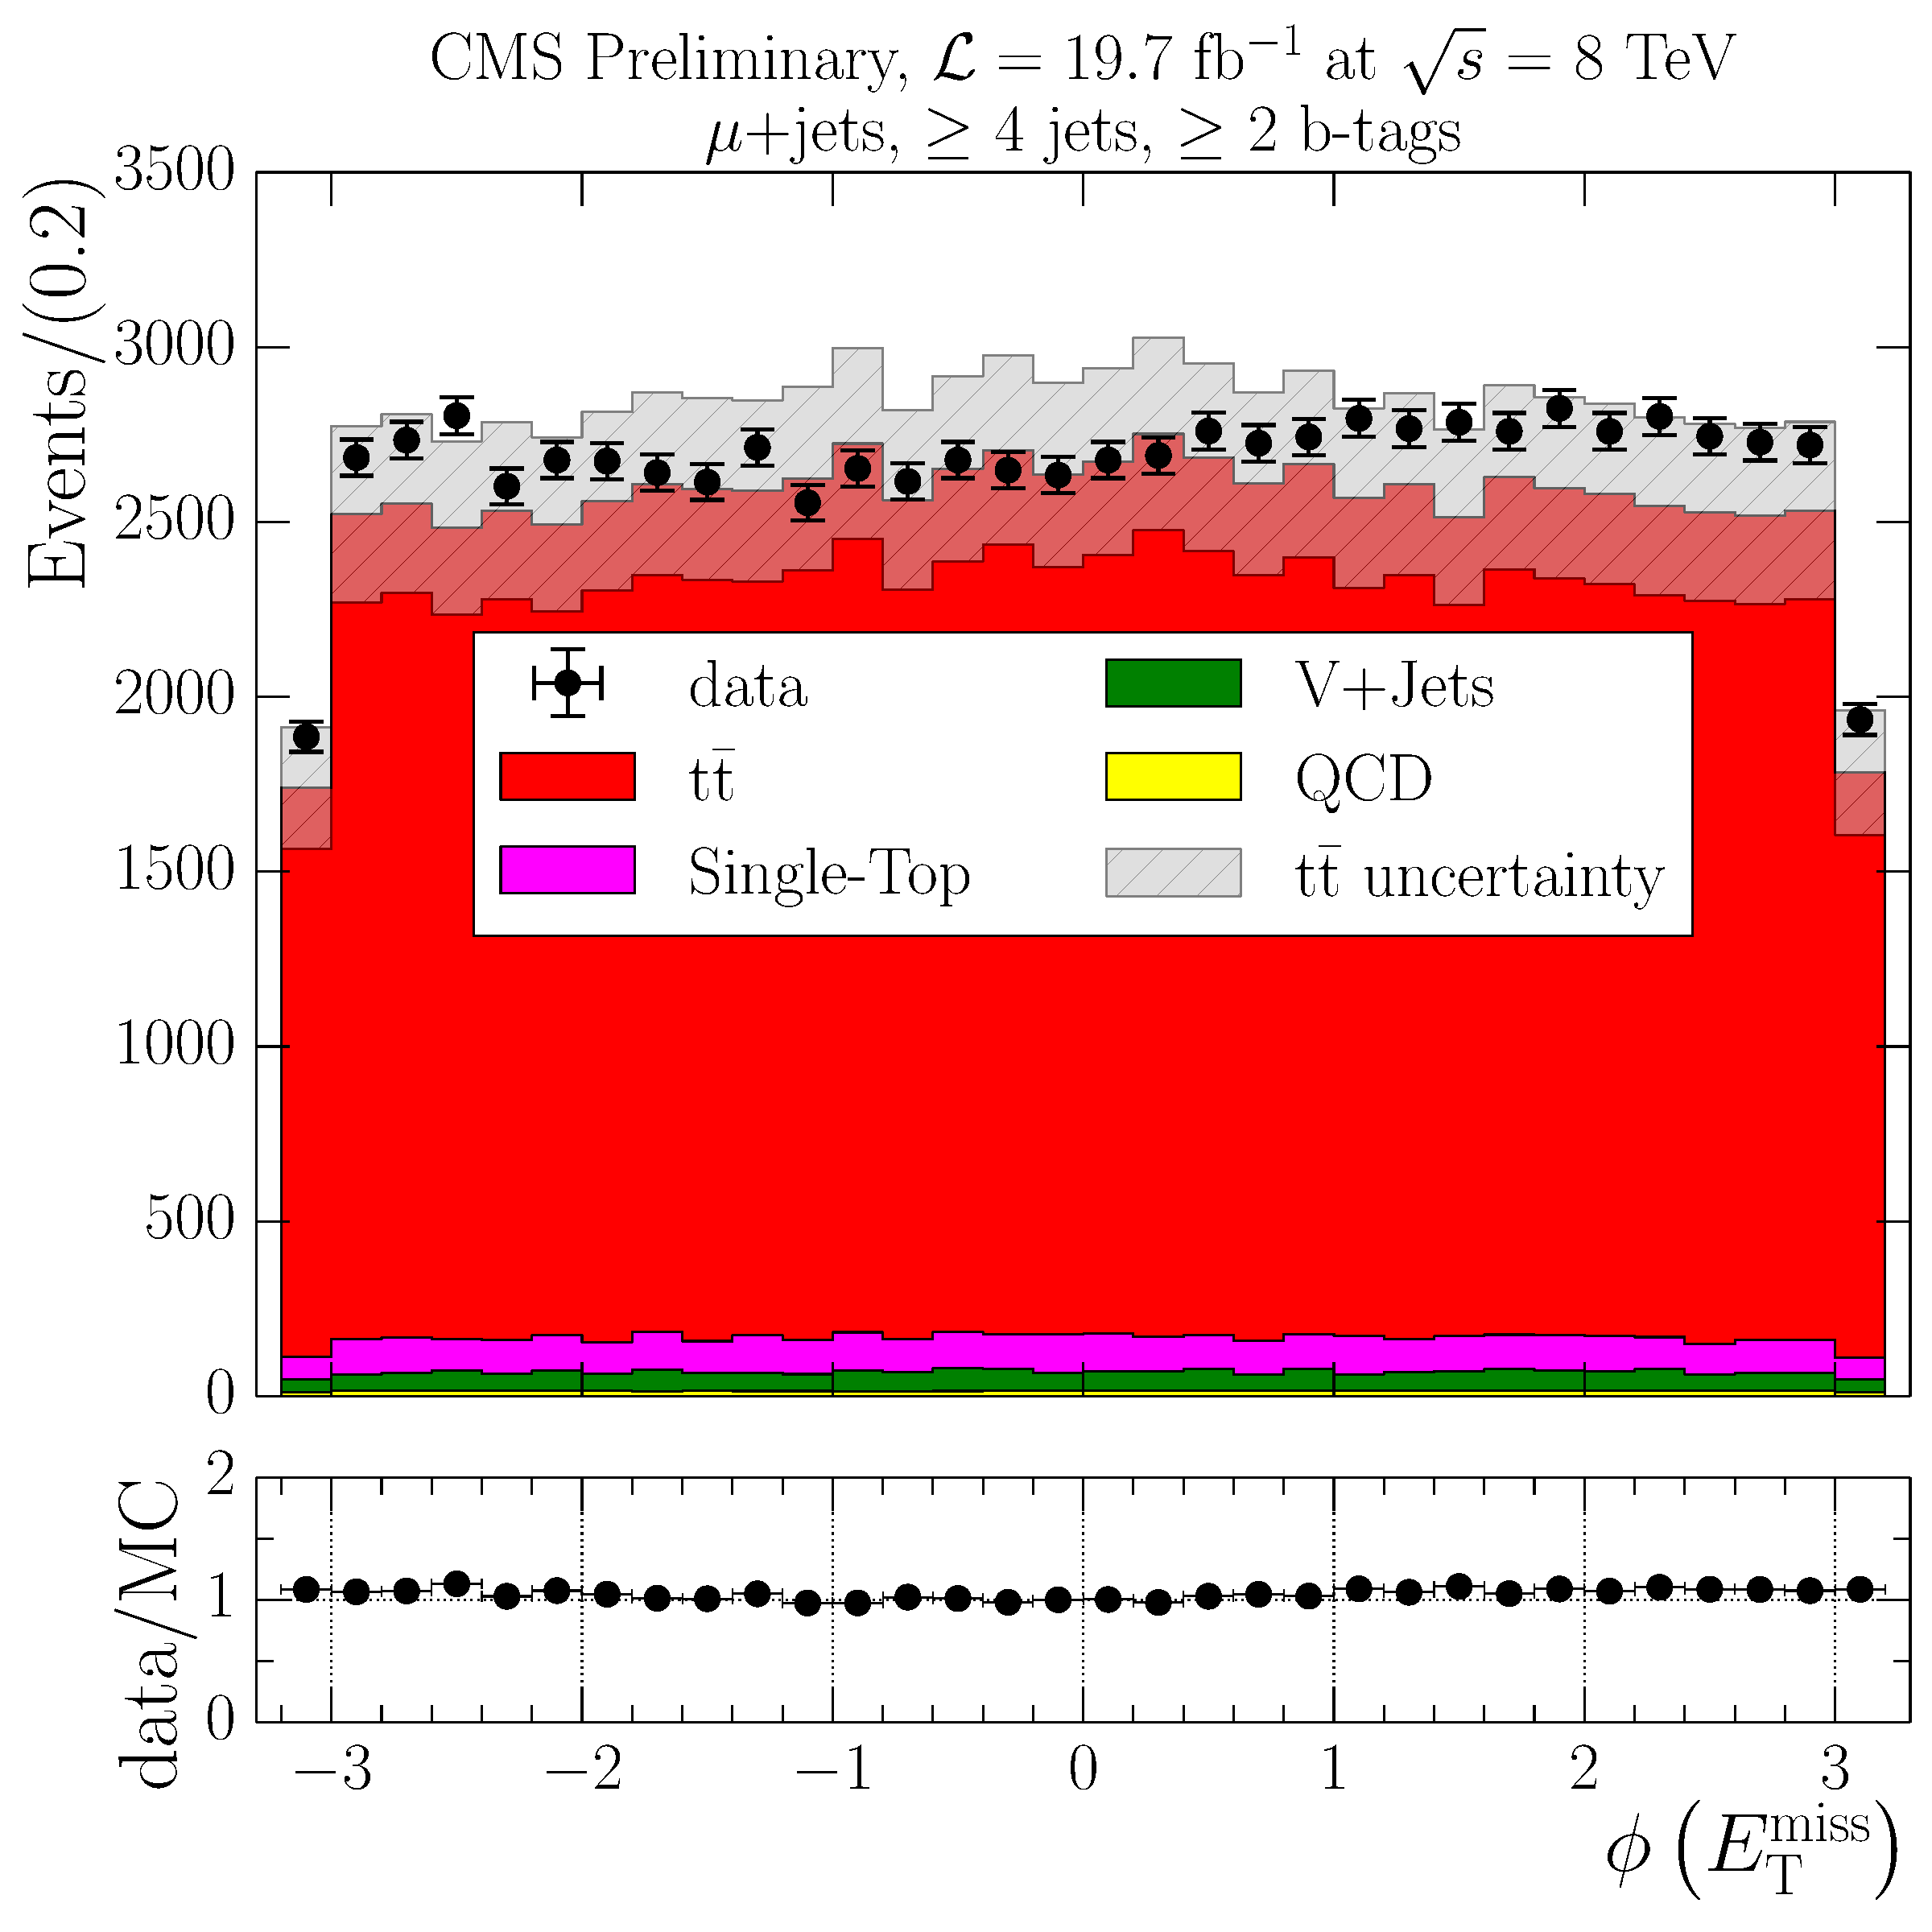
\includegraphics[width=0.50\textwidth]{control_plots/MuPlusJets_patType1CorrectedPFMet_phi_2orMoreBtags_with_ratio}} \\
  	\subfloat[]{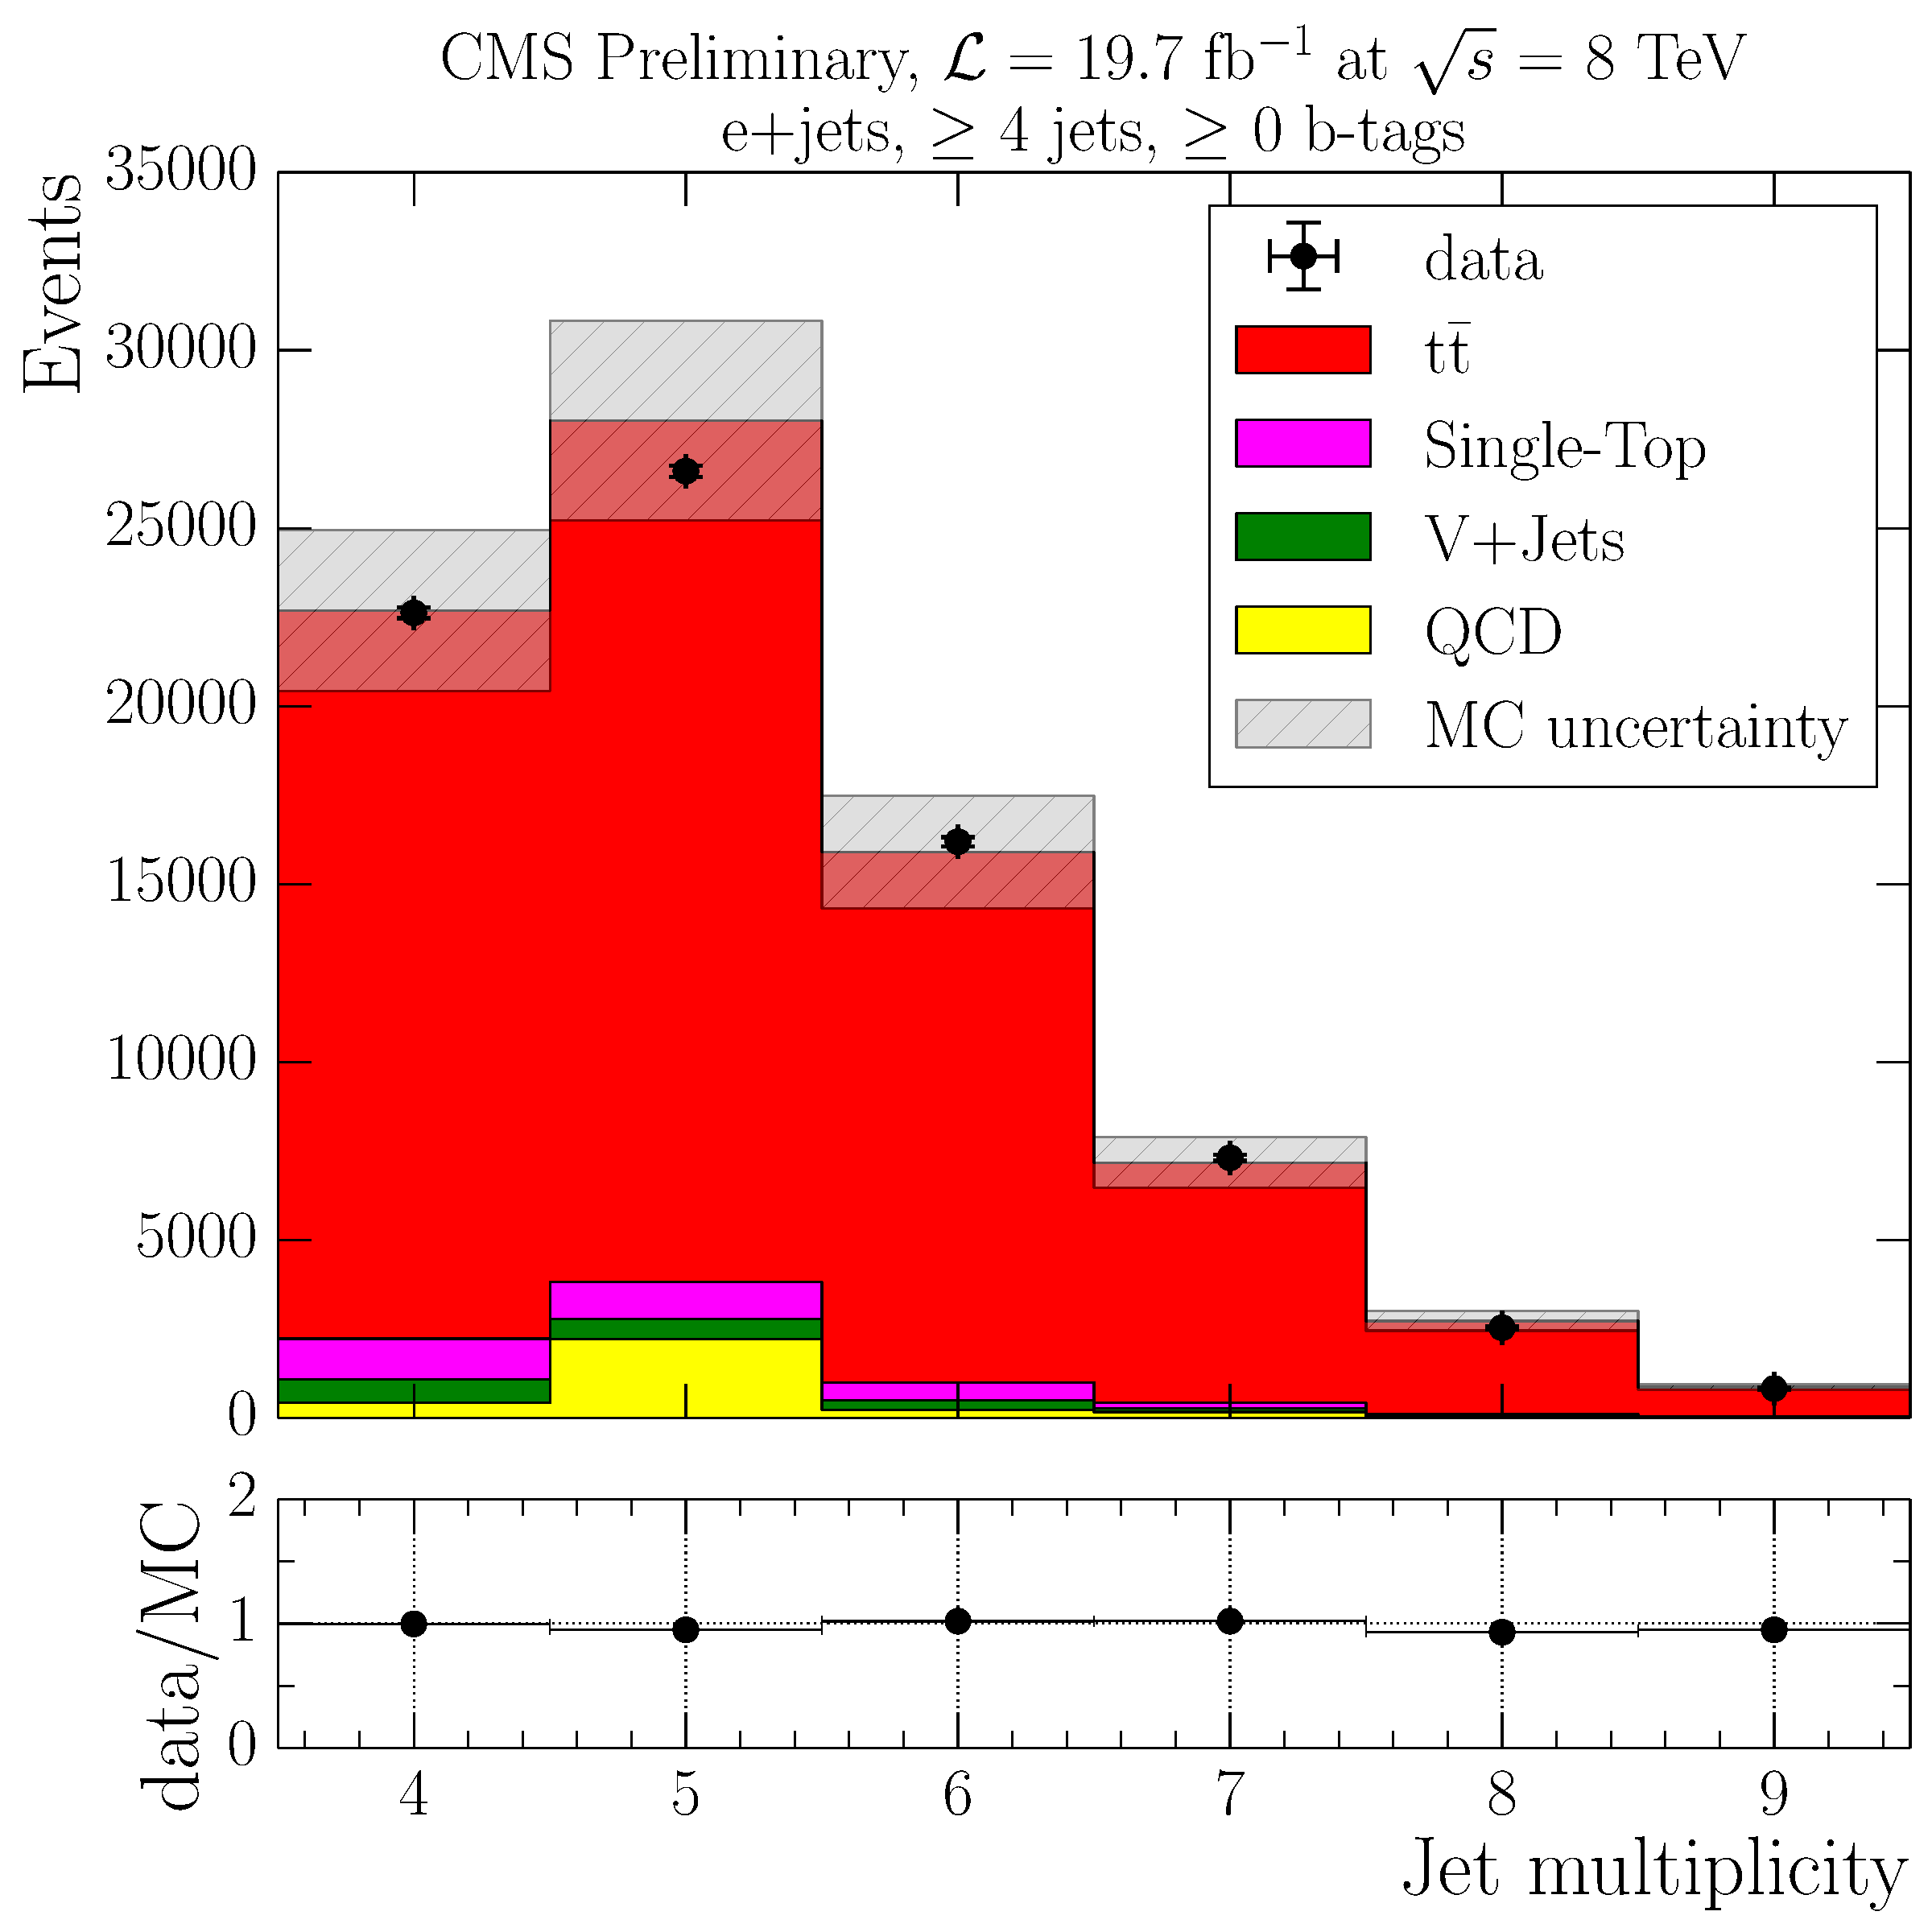
\includegraphics[width=0.50\textwidth]{control_plots/EPlusJets_N_Jets_2orMoreBtags_with_ratio}}\hfill
  	\subfloat[]{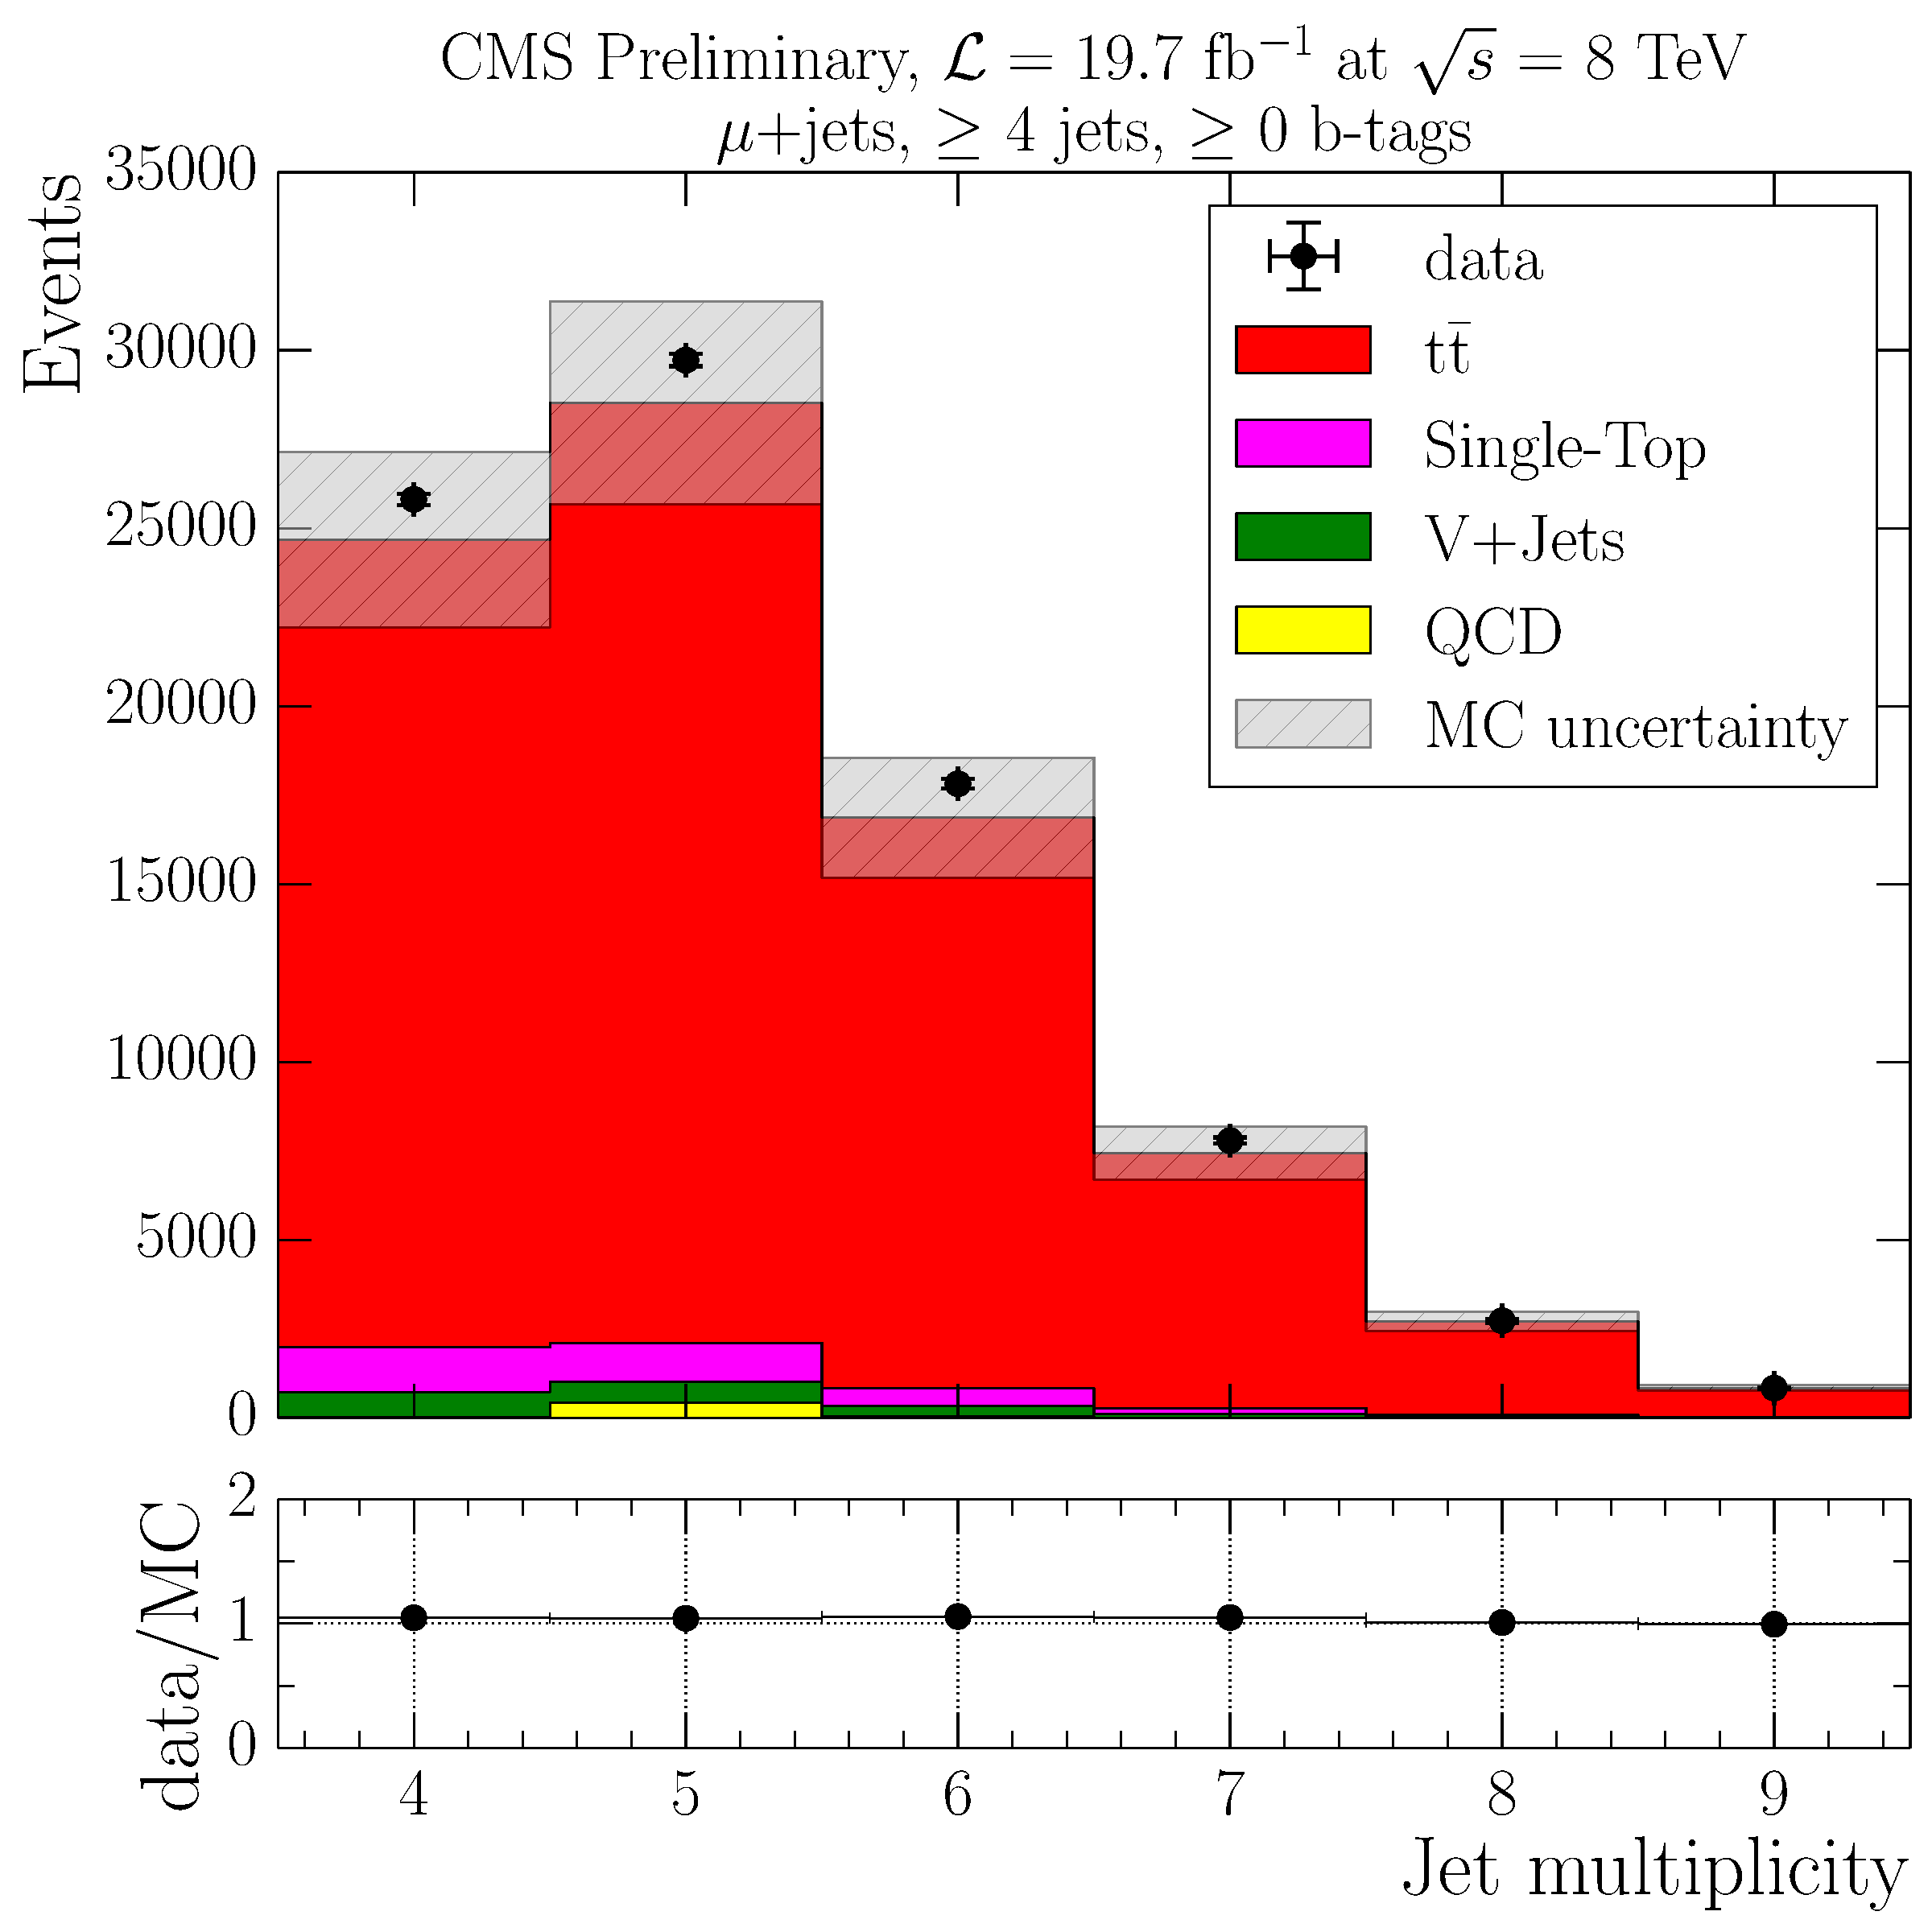
\includegraphics[width=0.50\textwidth]{control_plots/MuPlusJets_N_Jets_2orMoreBtags_with_ratio}} \\
    \caption[Data/MC comparison plots of $\phi(\MET)$ and jet multiplicity after the final event selection]{Data/MC
    comparison plots of $\phi(\MET)$ (a, b) and jet multiplicity (c, d) after the final event selection. Left-hand
    plots: electron plus jets selection, right-hand plots: muon plus jets selection.}
    \label{fig:contol_plots_phiMET_NJets}
\end{figure}

\newpage

\section{Differential cross section measurement}
\label{s_xsection:measurement}

\subsection{Primary variables}
\label{ss_xsection:variables}

In this analysis, the normalised differential cross section of \ttbar production is studied with respect to five primary
variables:

\begin{itemize}
	\item \MET, or magnitude of missing transverse momentum;
	\item \HT, or scalar sum of jet transverse momenta;
	\item \ST, or scalar sum of the transverse momenta of all objects in the event;
	\item \MT, or transverse mass of the leptonically decaying \W boson;
	\item \WPT, or magnitude of transverse momentum of the leptonically decaying \W boson.
\end{itemize}

These observables are often called event-level (or global) variables due to the fact that no high-level kinematic
reconstruction (e.g.\ that of a \ttbar pair) is required to calculate them. A lower level of complexity makes these
variables less prone to inefficiencies, systematic errors or biases arising from various kinematic reconstruction
techniques. Hence, global variables can provide better sensitivity in comparison of different theoretical models or
generator tunes.

\METvec is commonly referred to as the missing transverse energy, which is equivalent to missing transverse momentum
under assumption that the missing particles contributing to \METvec are massless. \METvec is defined as the negative of
the vector sum of the transverse momenta of all reconstructed particles in an event. Therefore, its direction is
opposite to the observed sum of transverse momentum, and its magnitude \MET is given by:
\[ \MET = - \left[ \left(\sum_i{p_{x}^i}\right)^2 + \left(\sum_i{p_{y}^i}\right)^2 \right]^{\frac{1}{2}}\]
where the sums are calculated over all measured particles in the event.

\HT is defined as the scalar sum of the transverse momenta of all reconstructed jets in the event:
\[\HT = \sum_{\mathrm{all~jets}}\pt^{\mathrm{jet}}\]
Here all jets are required to have a \pt $>$ \SI{20}{\GeV} as described in Section~\ref{s_xsection:event_selection}.

\ST represents the sum of \HT, \MET and the magnitude of \pt of the single isolated lepton:
\[\ST = \HT + \MET + p_\mathrm{T}^\mathrm{lepton}\]

\WPT refers to the magnitude of transverse momentum of the leptonically decaying \W boson, which is calculated from the
single isolated lepton and \MET assumed to originate from the \ttbar decay:
\[\WPT = \sqrt{(p_x^{\mathrm{lepton}} + p_x^{\mathrm{miss}})^2 + (p_y^{\mathrm{lepton}} + p_y^{\mathrm{miss}})^2}\]

Finally, \MT is defined as the transverse mass of the leptonically decaying \W boson, also using the single isolated
lepton and \MET:
\[\MT = \sqrt{(\ET {}^{\mathrm{lepton}} +\met)^2 - \wpt {}^2}\]
where $\ET {}^{\mathrm{lepton}}$ denotes the transverse energy of the lepton.

\subsection{Choice of binning}
\label{ss_xsection:binning}

The choice of binning for primary variables is an important part of differential cross section measurement. It is
directly influenced by available statistics and detector resolution. An ideal measurement would benefit from the cross
section calculation in as many bins as possible. However, insufficient statistics leads to high statistical uncertainty
in a particular bin, whereas limited detector resolution causes substantial migration effects between bins. Bin
migration happens if an event originating from one bin appears in a different bin after reconstruction. Unreasonable
binning choice would lead to a high number of such events, which can potentially compromise the cross section
measurement.

To quantify the bin migration, purity and stability variables are introduced, defined as:
\begin{align}
p_i = \frac{N^{\rec\&\gen}_i}{N^{\rec}_i} \\
s_i = \frac{N^{\rec\&\gen}_i}{N^{\gen}_i}
\end{align}
where $N^{\rec\&\gen}_i$ is the number of events both generated and reconstructed in the same bin, and
$N^{\rec}_k$ ($N^{\gen}_i$) is the number of reconstructed (generated) events within a bin.

The purity $p_i$ quantifies migration into a bin $i$, whereas the stability $s_i$ is sensitive to migration out of a
bin. The binning is chosen in such way that both purity and stability are above \num{0.5}, or do not fall far below this
value. This process is performed for both electron and muon channels, and common binning is derived in order to be able
to combine both channels in the final cross section measurement.

Figure~\ref{fig:choice_of_bins_MET} shows the two-dimensional distributions of reconstructed versus generated \MET,
which were used to calculate purity and stability. The distributions were obtained with the central signal
\ttbar sample. Red lines represent the bin edges for the chosen binning. Tables~\ref{tab:binning_MET_electron} and
\ref{tab:binning_MET_muon} show the numerical values of purity and stability, as well as the selected binning for \MET
variable. Results for other primary variables can be found in Appendix~\ref{a:binning}.

\begin{table}[htp]
  	\centering
  	\caption[Stability and purity of chosen \MET bins in the electron channel]{Stability and purity of chosen \MET bins
  	in the electron channel for \ttbar MC events}
  	\label{tab:binning_MET_electron}
	\resizebox{\columnwidth}{!}{
	\begin{tabular}{@{}lrrrrrr@{}}
	\toprule
	bin, \GeV & $0 < \MET < 25$ & $25 \leq \MET < 45$ & $45 \leq \MET < 75$ & $75 \leq \MET <100$ & $100 \leq \MET <150$ & $\MET \geq 150$ \\
	\midrule 
	events &  10337 & 17982 & 19503 & 12594 & 7220 & 2832\\
	purity & 0.52 & 0.48 & 0.44 & 0.42 & 0.54 & 0.69\\
	stability & 0.42 & 0.41 & 0.47 & 0.52 & 0.66 & 0.86  \\
	\bottomrule
	\end{tabular}
	}
\end{table}


\begin{table}[htp]
  	\centering
  	\caption[Stability and purity of chosen \MET bins in the muon channel]{Stability and purity of chosen \MET bins in
  	the muon channel for \ttbar MC events}
  	\label{tab:binning_MET_muon}
	\resizebox{\columnwidth}{!}{
	\begin{tabular}{@{}lrrrrrr@{}}
	\toprule
	bin, \GeV & $0 < \MET < 25$ & $25 \leq \MET < 45$ & $45 \leq \MET < 75$ & $75 \leq \MET <100$ & $100 \leq \MET <150$ & $\MET \geq 150$ \\
	\midrule 
	events & 11506 & 20348 & 22594 & 14413 & 8417 & 3274\\
	purity & 0.52 & 0.49 & 0.45 & 0.42 & 0.52 & 0.69\\
	stability & 0.43 & 0.42 & 0.47 & 0.5 & 0.66 & 0.87\\
	\bottomrule
	\end{tabular}
	}
\end{table}

\begin{figure}[!htbp]
	\centering
	\subfloat[]{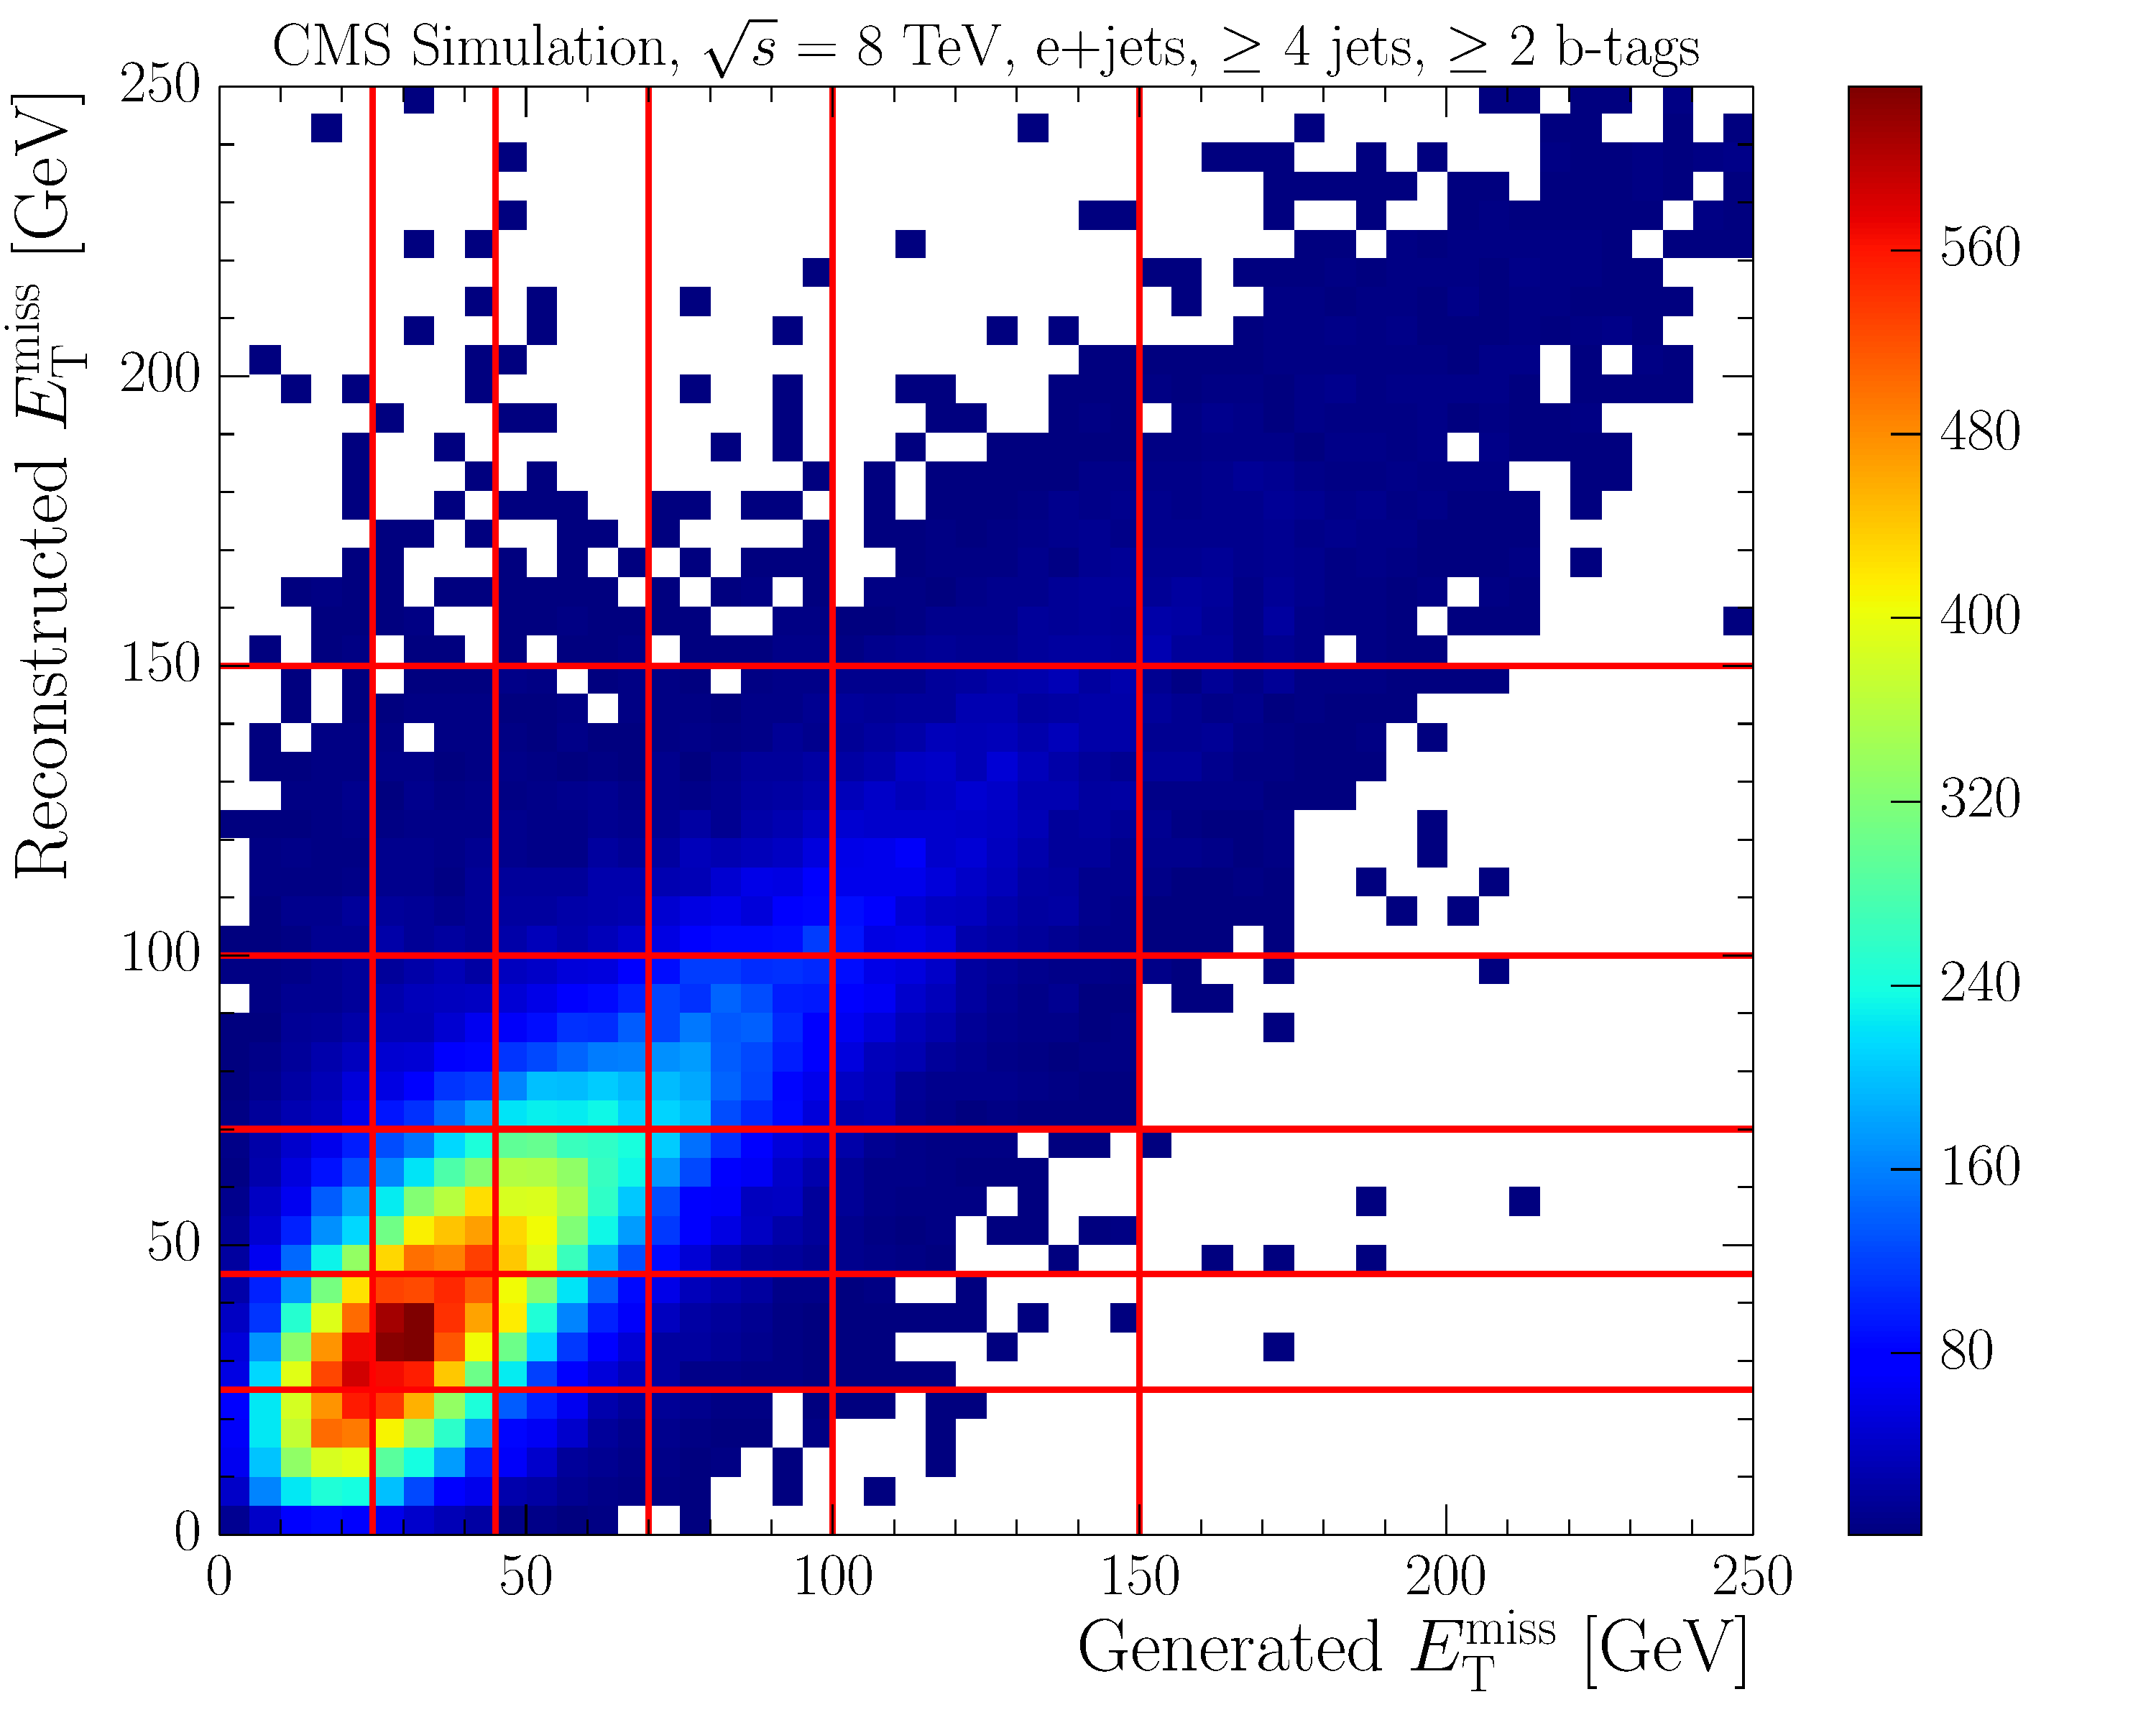
\includegraphics[width=0.5\textwidth]{binning/EPlusJets_MET}}\hfill
	\subfloat[]{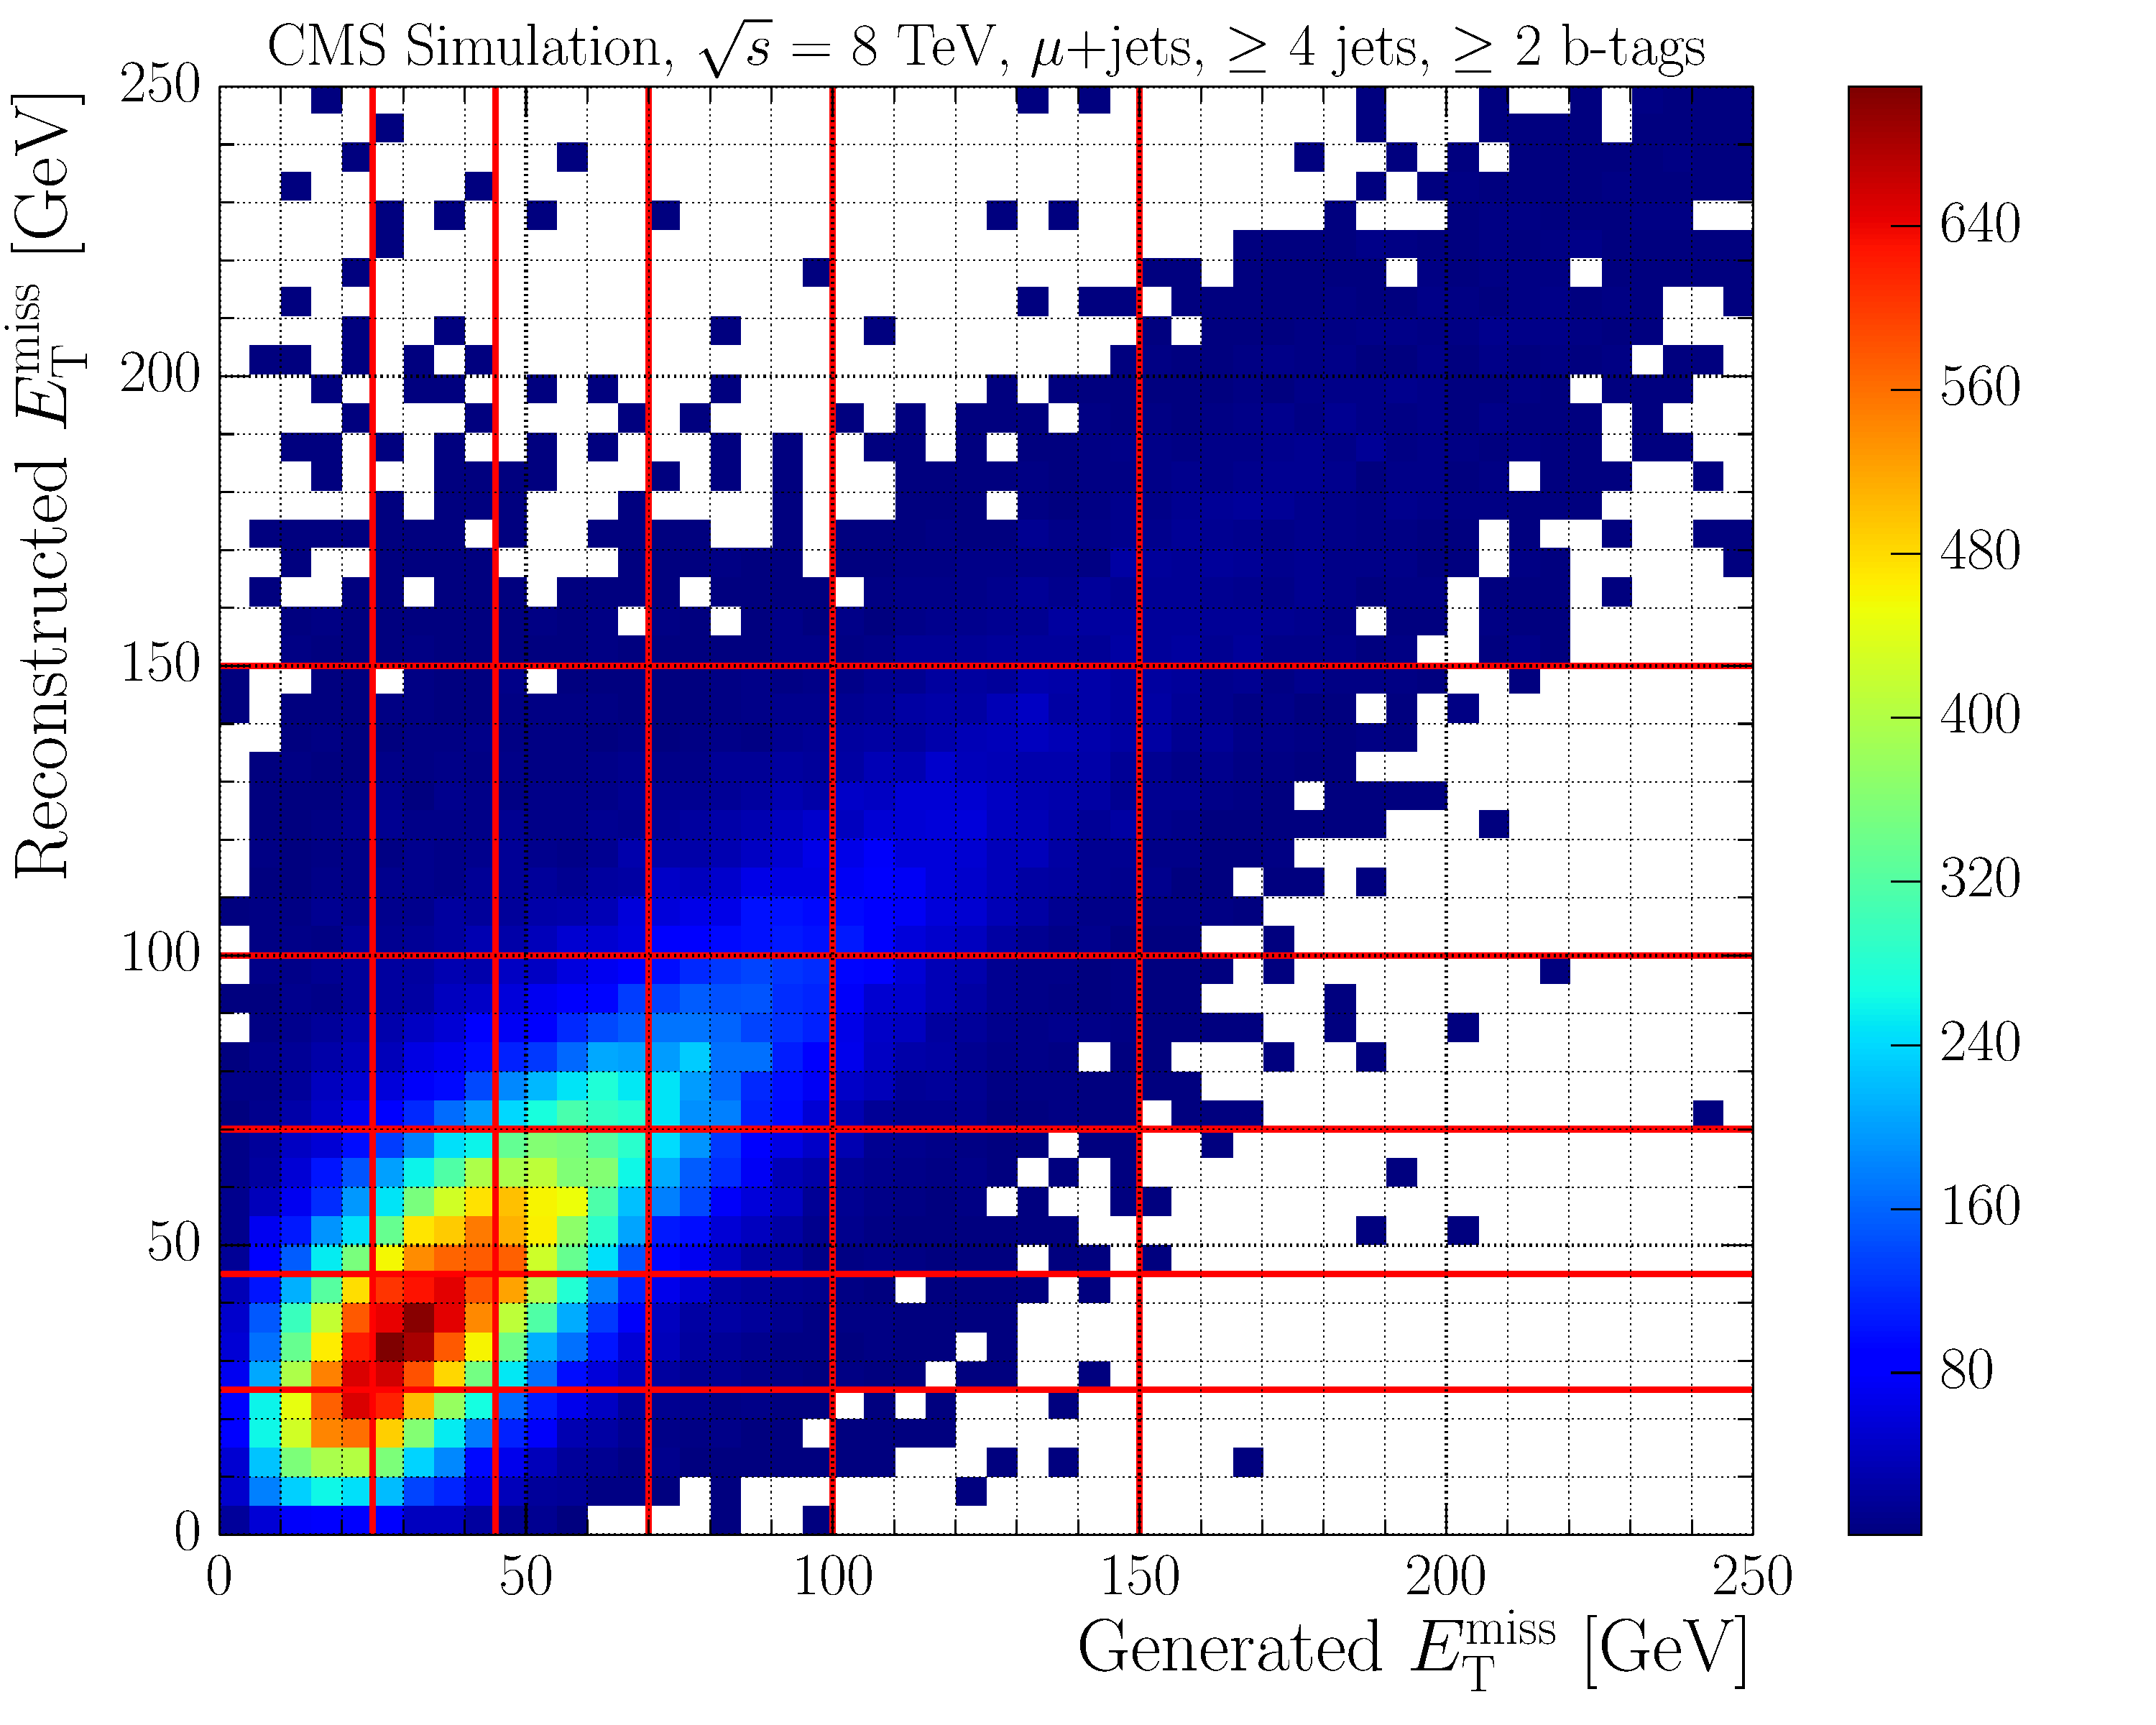
\includegraphics[width=0.5\textwidth]{binning/MuPlusJets_MET}}\\
	\caption[Reconstructed versus generated \MET]{Reconstructed versus generated \MET for electron plus jets (a) and
	muon plus jets events (b).}
	\label{fig:choice_of_bins_MET}
 \end{figure}

\subsection{Fitting procedure}
\label{ss_xsection:fitting}
To calculate the differential cross section as a function of a primary variable, the number of signal \ttbar events has
to be measured in each primary variable bin. For this purpose, a template fit of the observed distribution of lepton
pseudorapidity ($\abs {\eta_l}$) is performed in each bin in order to estimate the number of \ttbar events by
subtracting the primary backgrounds. Three separate normalised templates are produced for the input of the template fit:

\begin{itemize}
	\item $\abs {\eta_l}$ distribution of top-like events, i.e.\ combined template of \ttbar and single top MC;
	\item $\abs {\eta_l}$ distribution of \VpJets events, i.e.\ combined \WpJets and \ZpJets templates;
	\item $\abs {\eta_l}$ shape of QCD events, estimated from data (Section~\ref{s_xsection:data_driven_QCD}).
\end{itemize}

The combination of \WpJets and \ZpJets templates is justified by the similarity of the shapes of distributions, as well
as by limited MC statistics. Figures~\ref{fig:fit_templates_MET_electron} and \ref{fig:fit_templates_MET_muon} show
templates for the \MET variable for electron and muon channels, respectively. Templates for other primary variables are
attached in Appendix~\ref{a:templates}.

\sisetup{range-phrase = --}
\sisetup{range-units = single}

\begin{figure}[!htbp]
	\centering
	\vspace*{-0.5cm}
	\hspace*{\fill}
  	{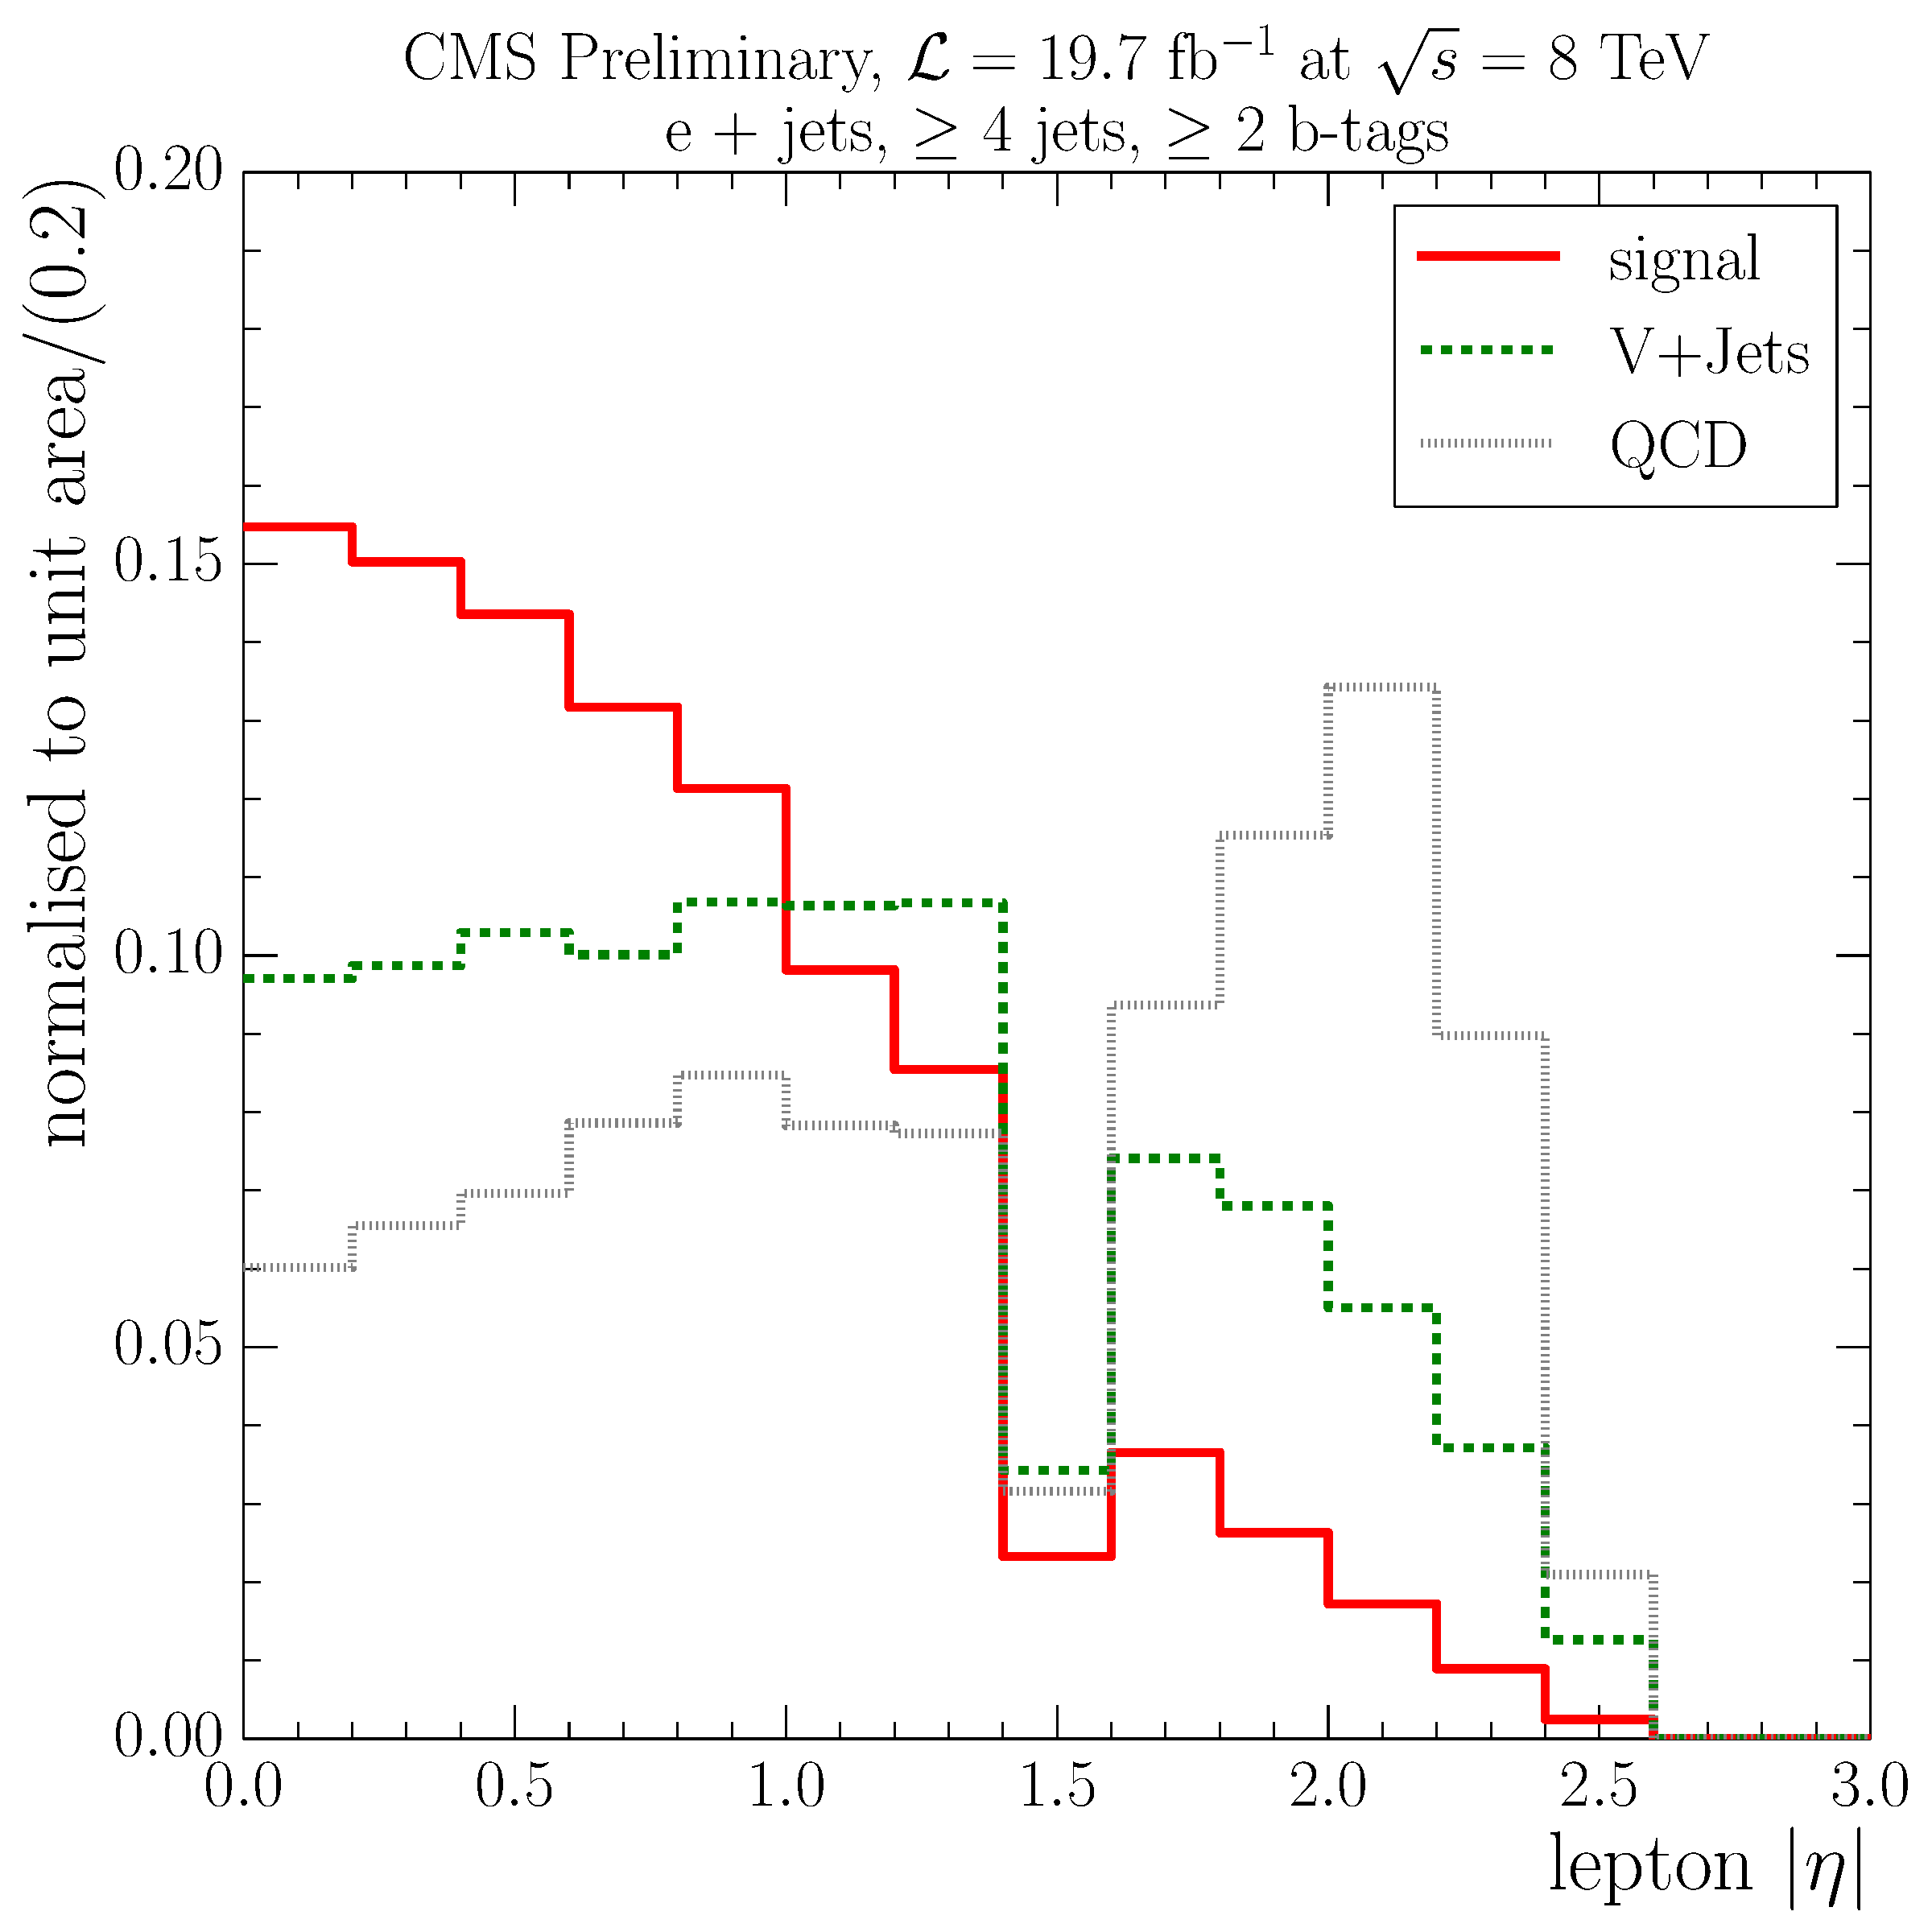
\includegraphics[width=0.42\textwidth]{measurement/MET/central/fit_templates/electron_templates_bin_0-25}}\hfill
  	{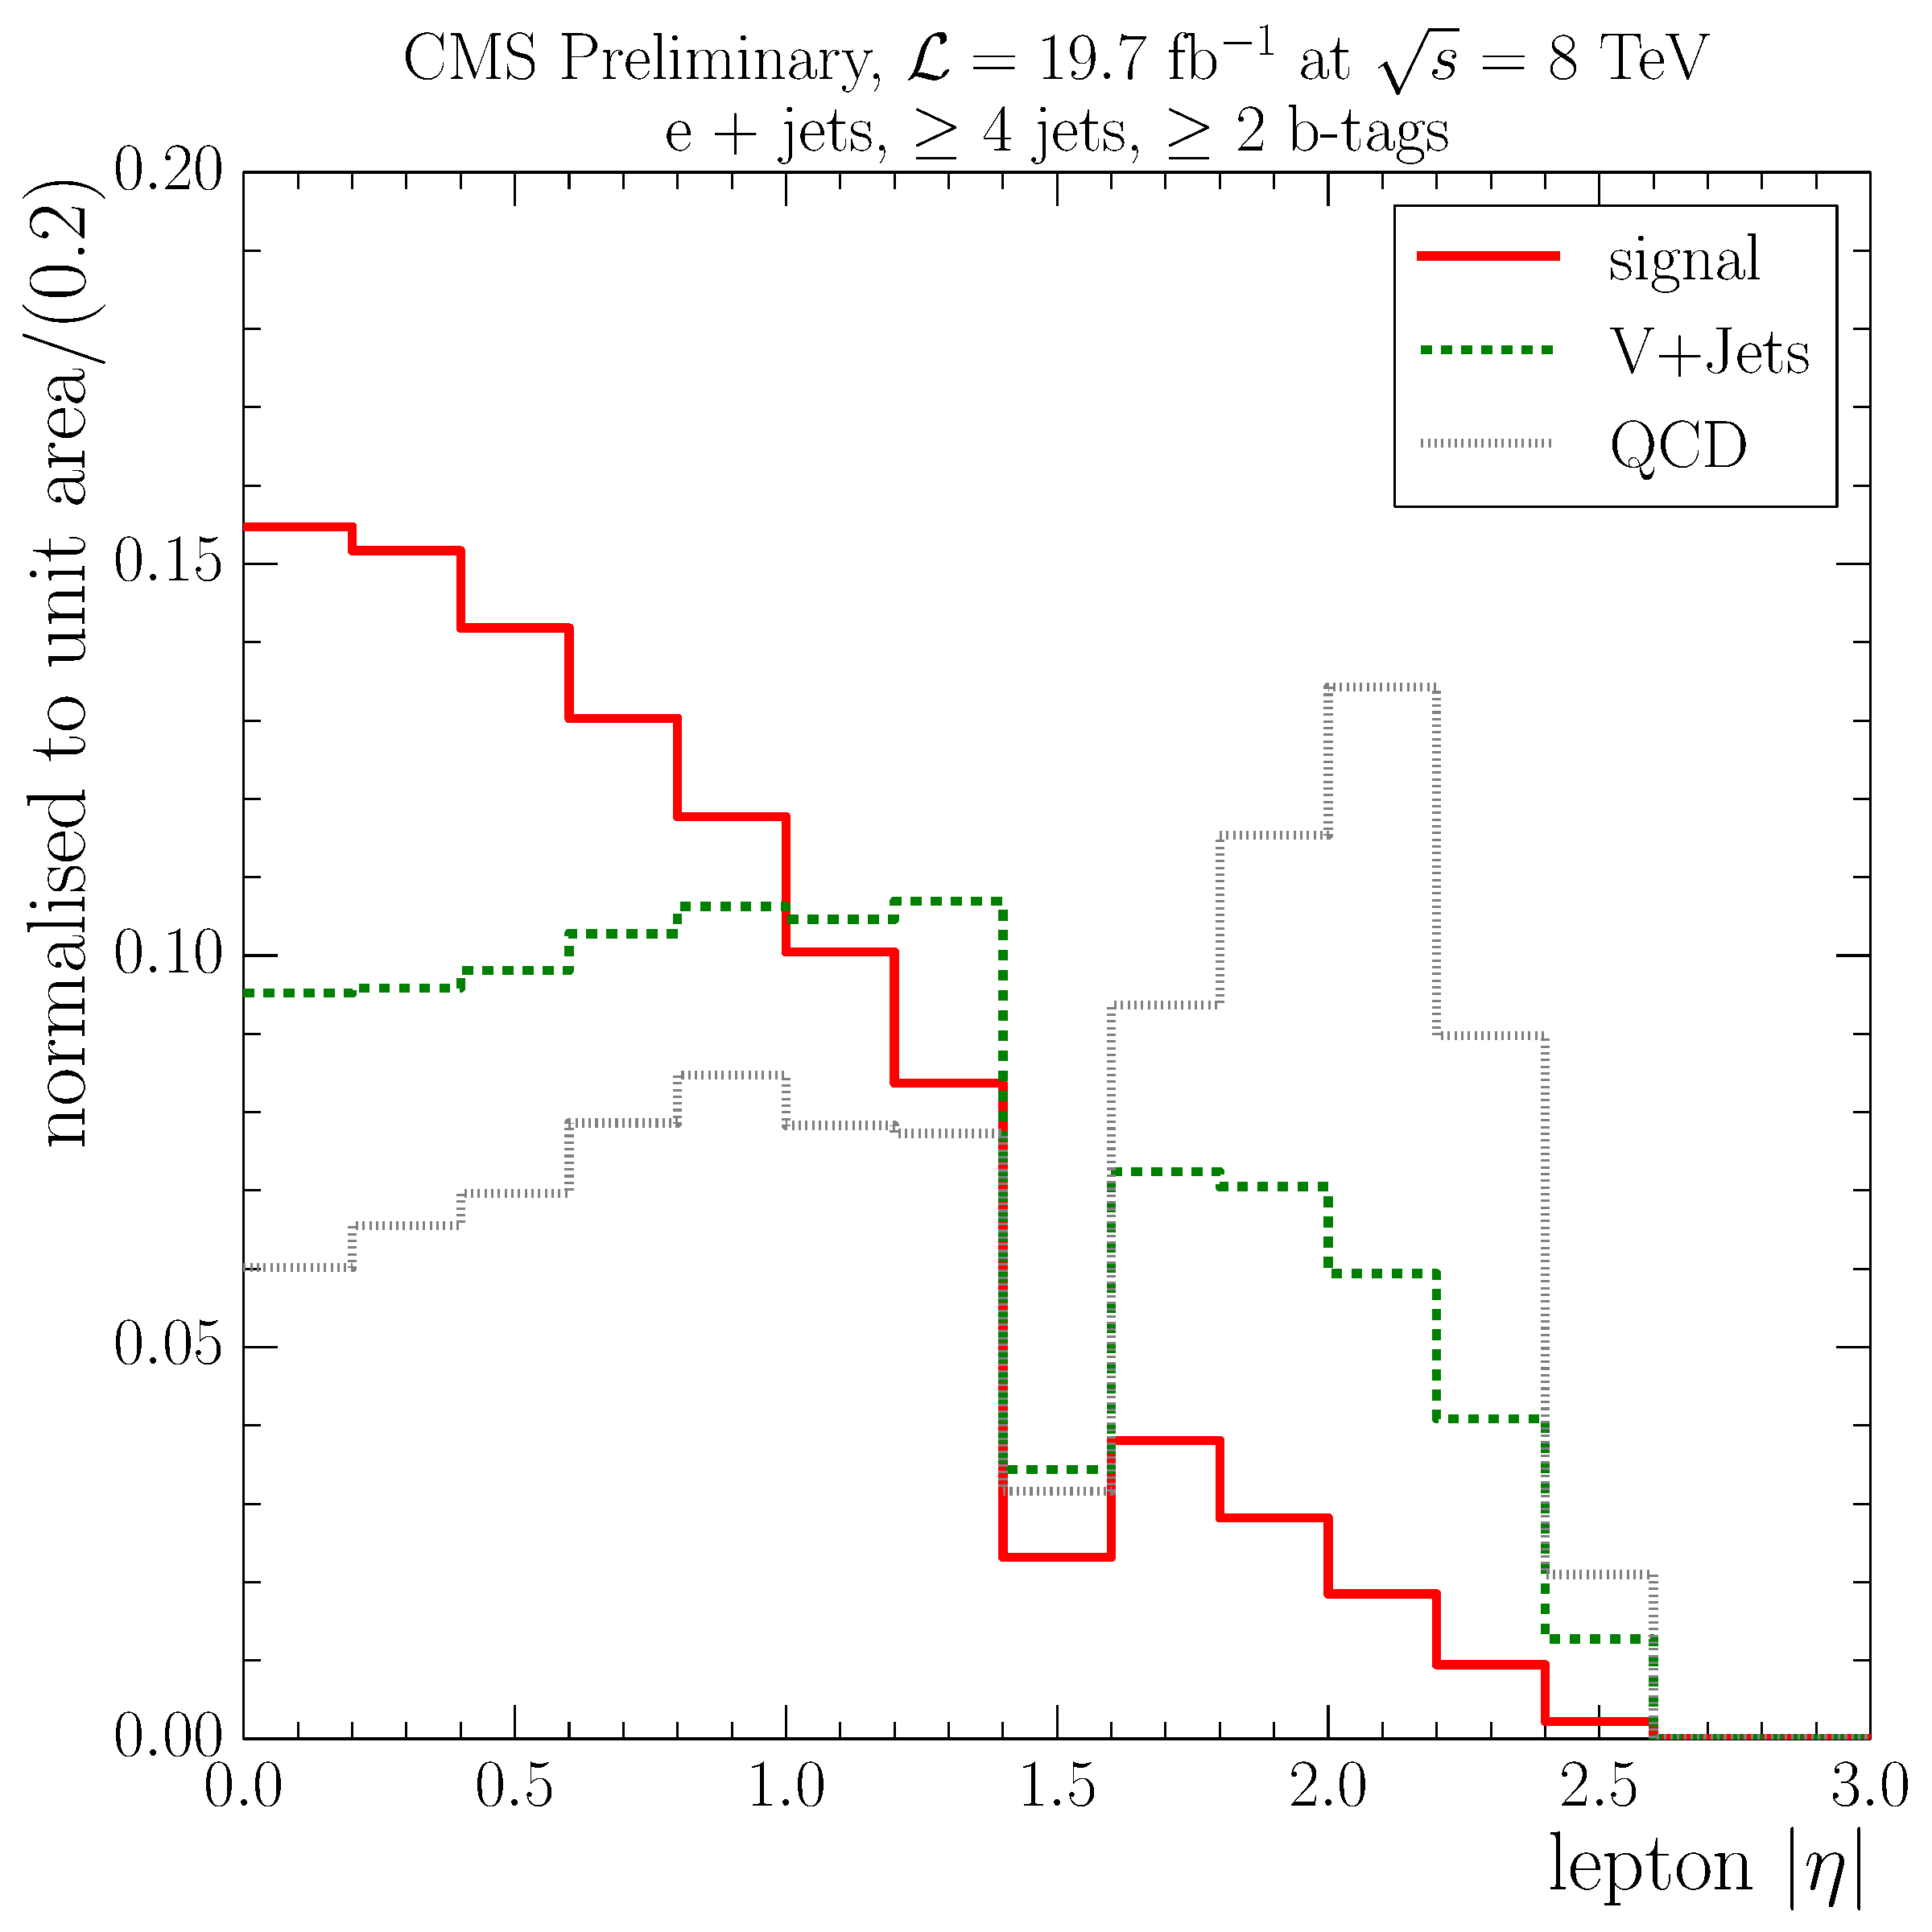
\includegraphics[width=0.42\textwidth]{measurement/MET/central/fit_templates/electron_templates_bin_25-45}}
  	\hspace*{\fill} \\
  	\hspace*{\fill}
  	{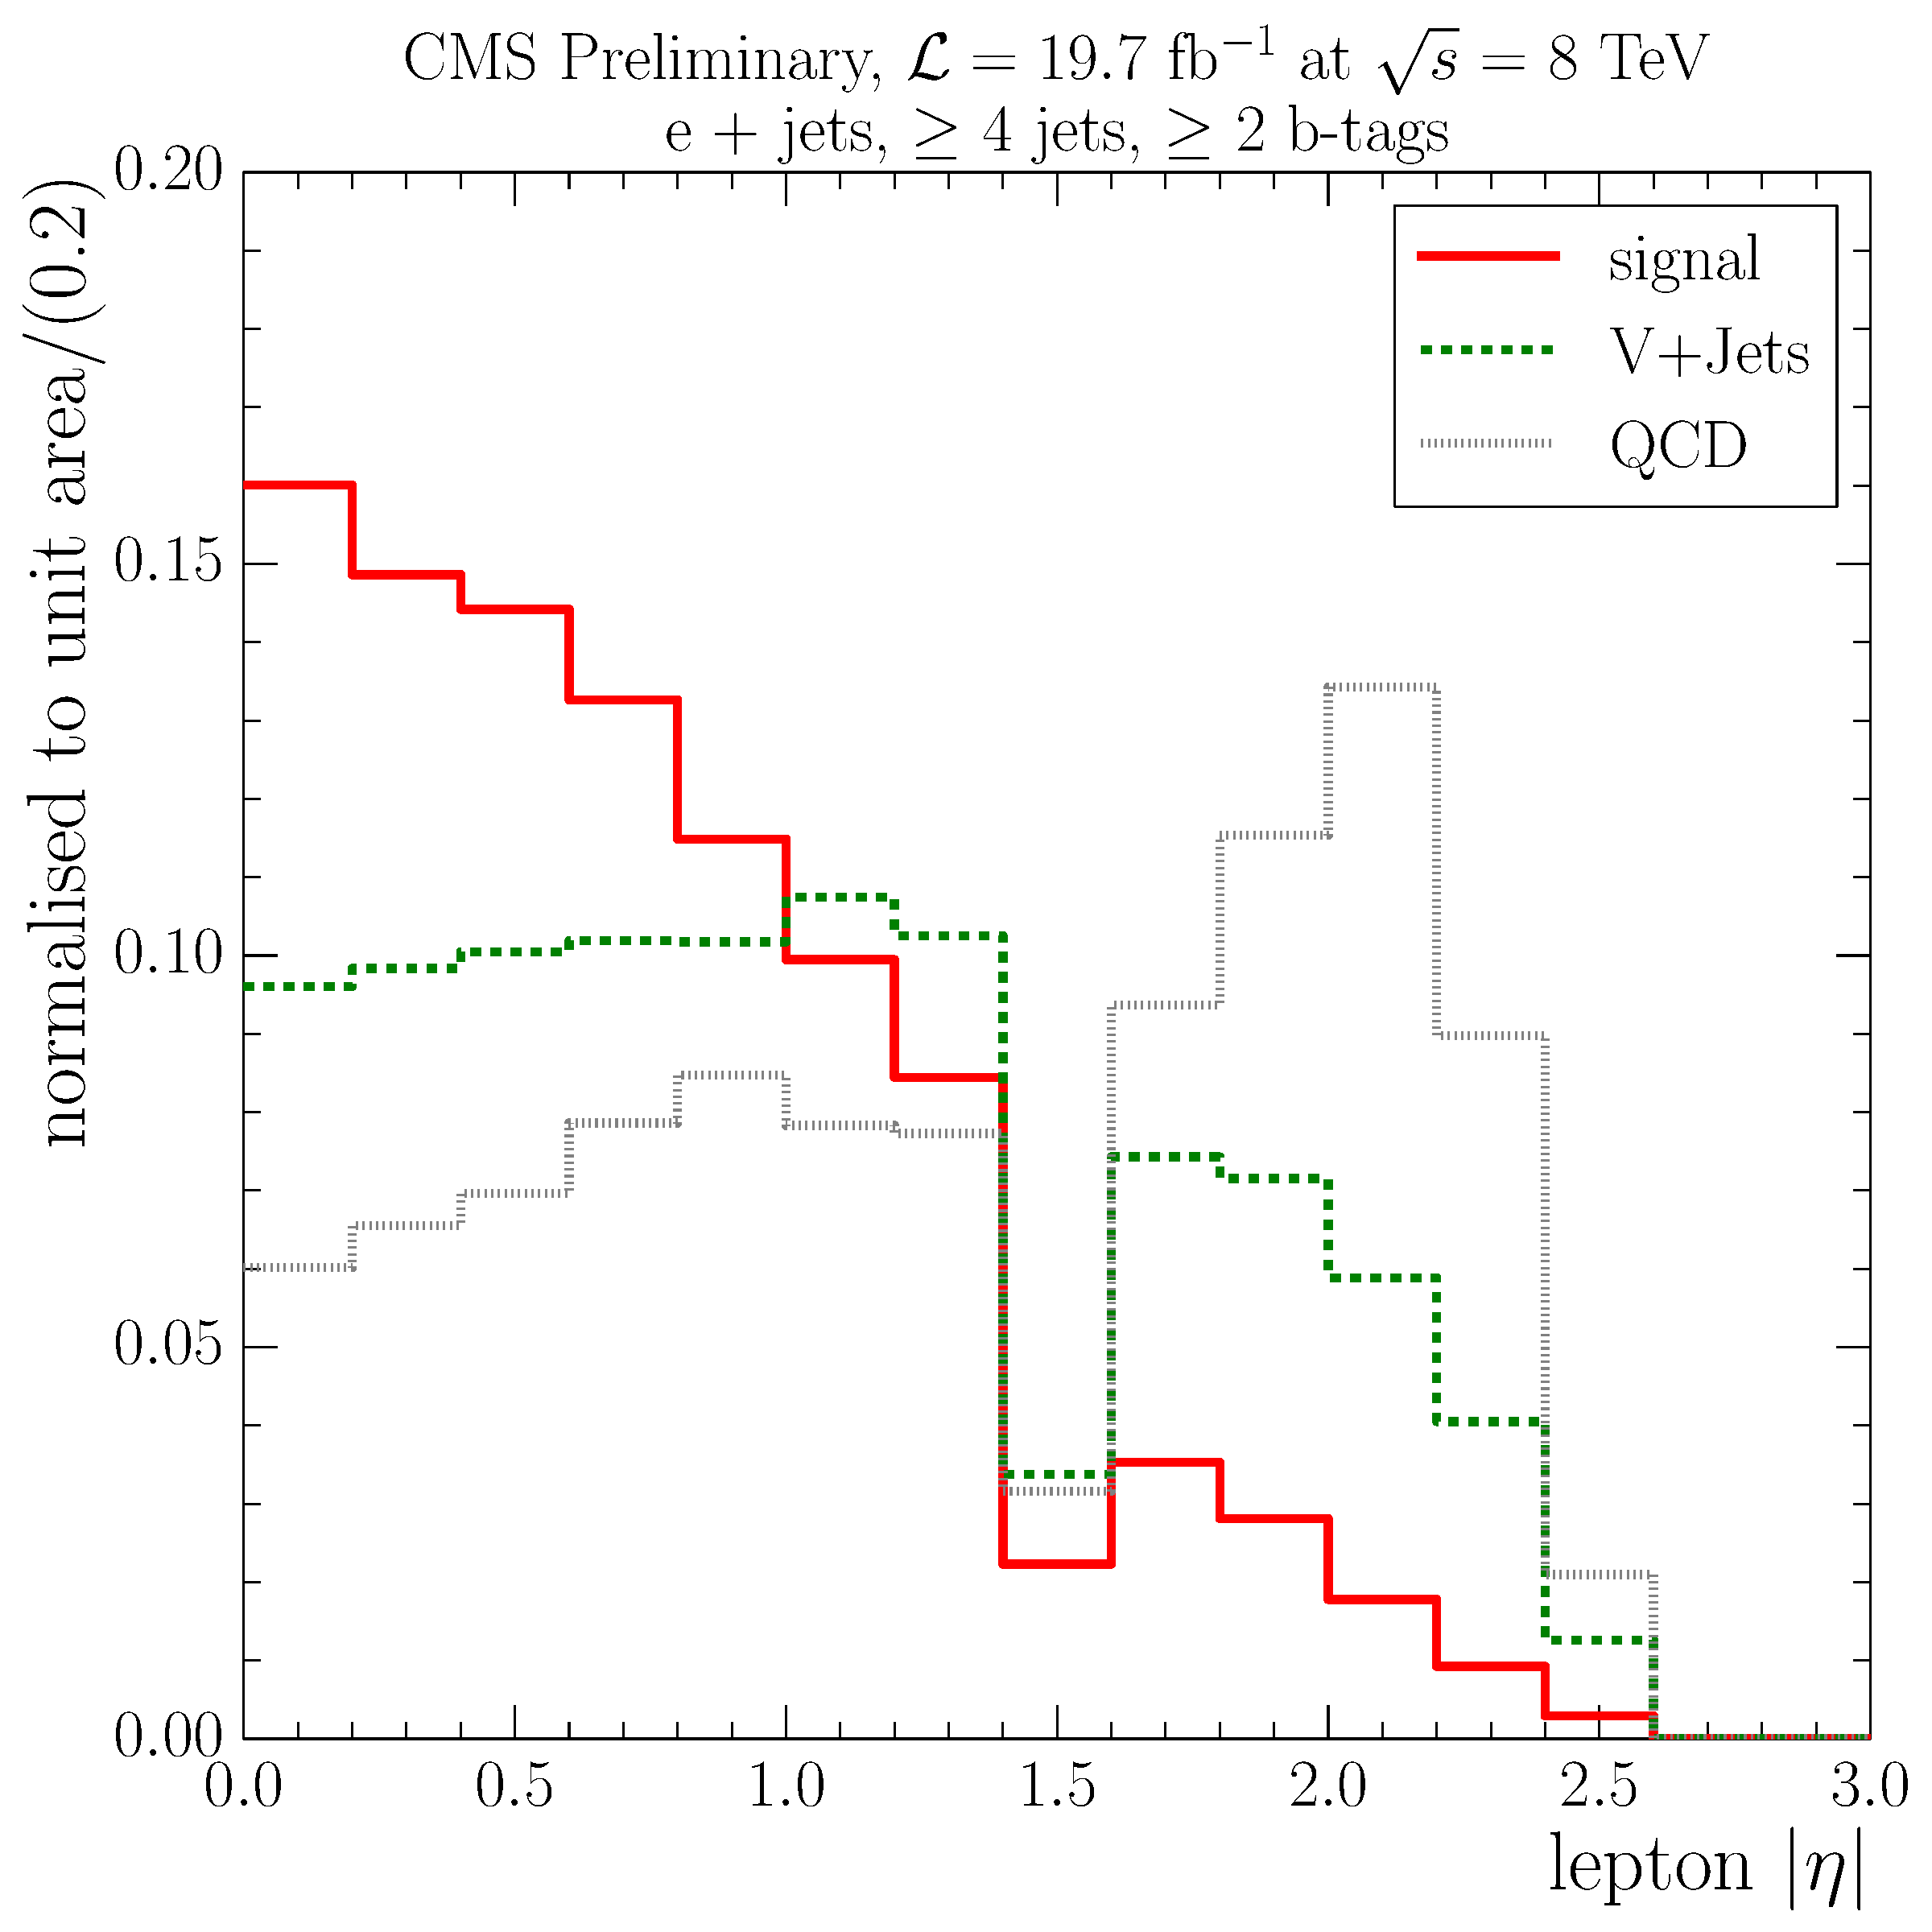
\includegraphics[width=0.42\textwidth]{measurement/MET/central/fit_templates/electron_templates_bin_45-70}}\hfill
  	{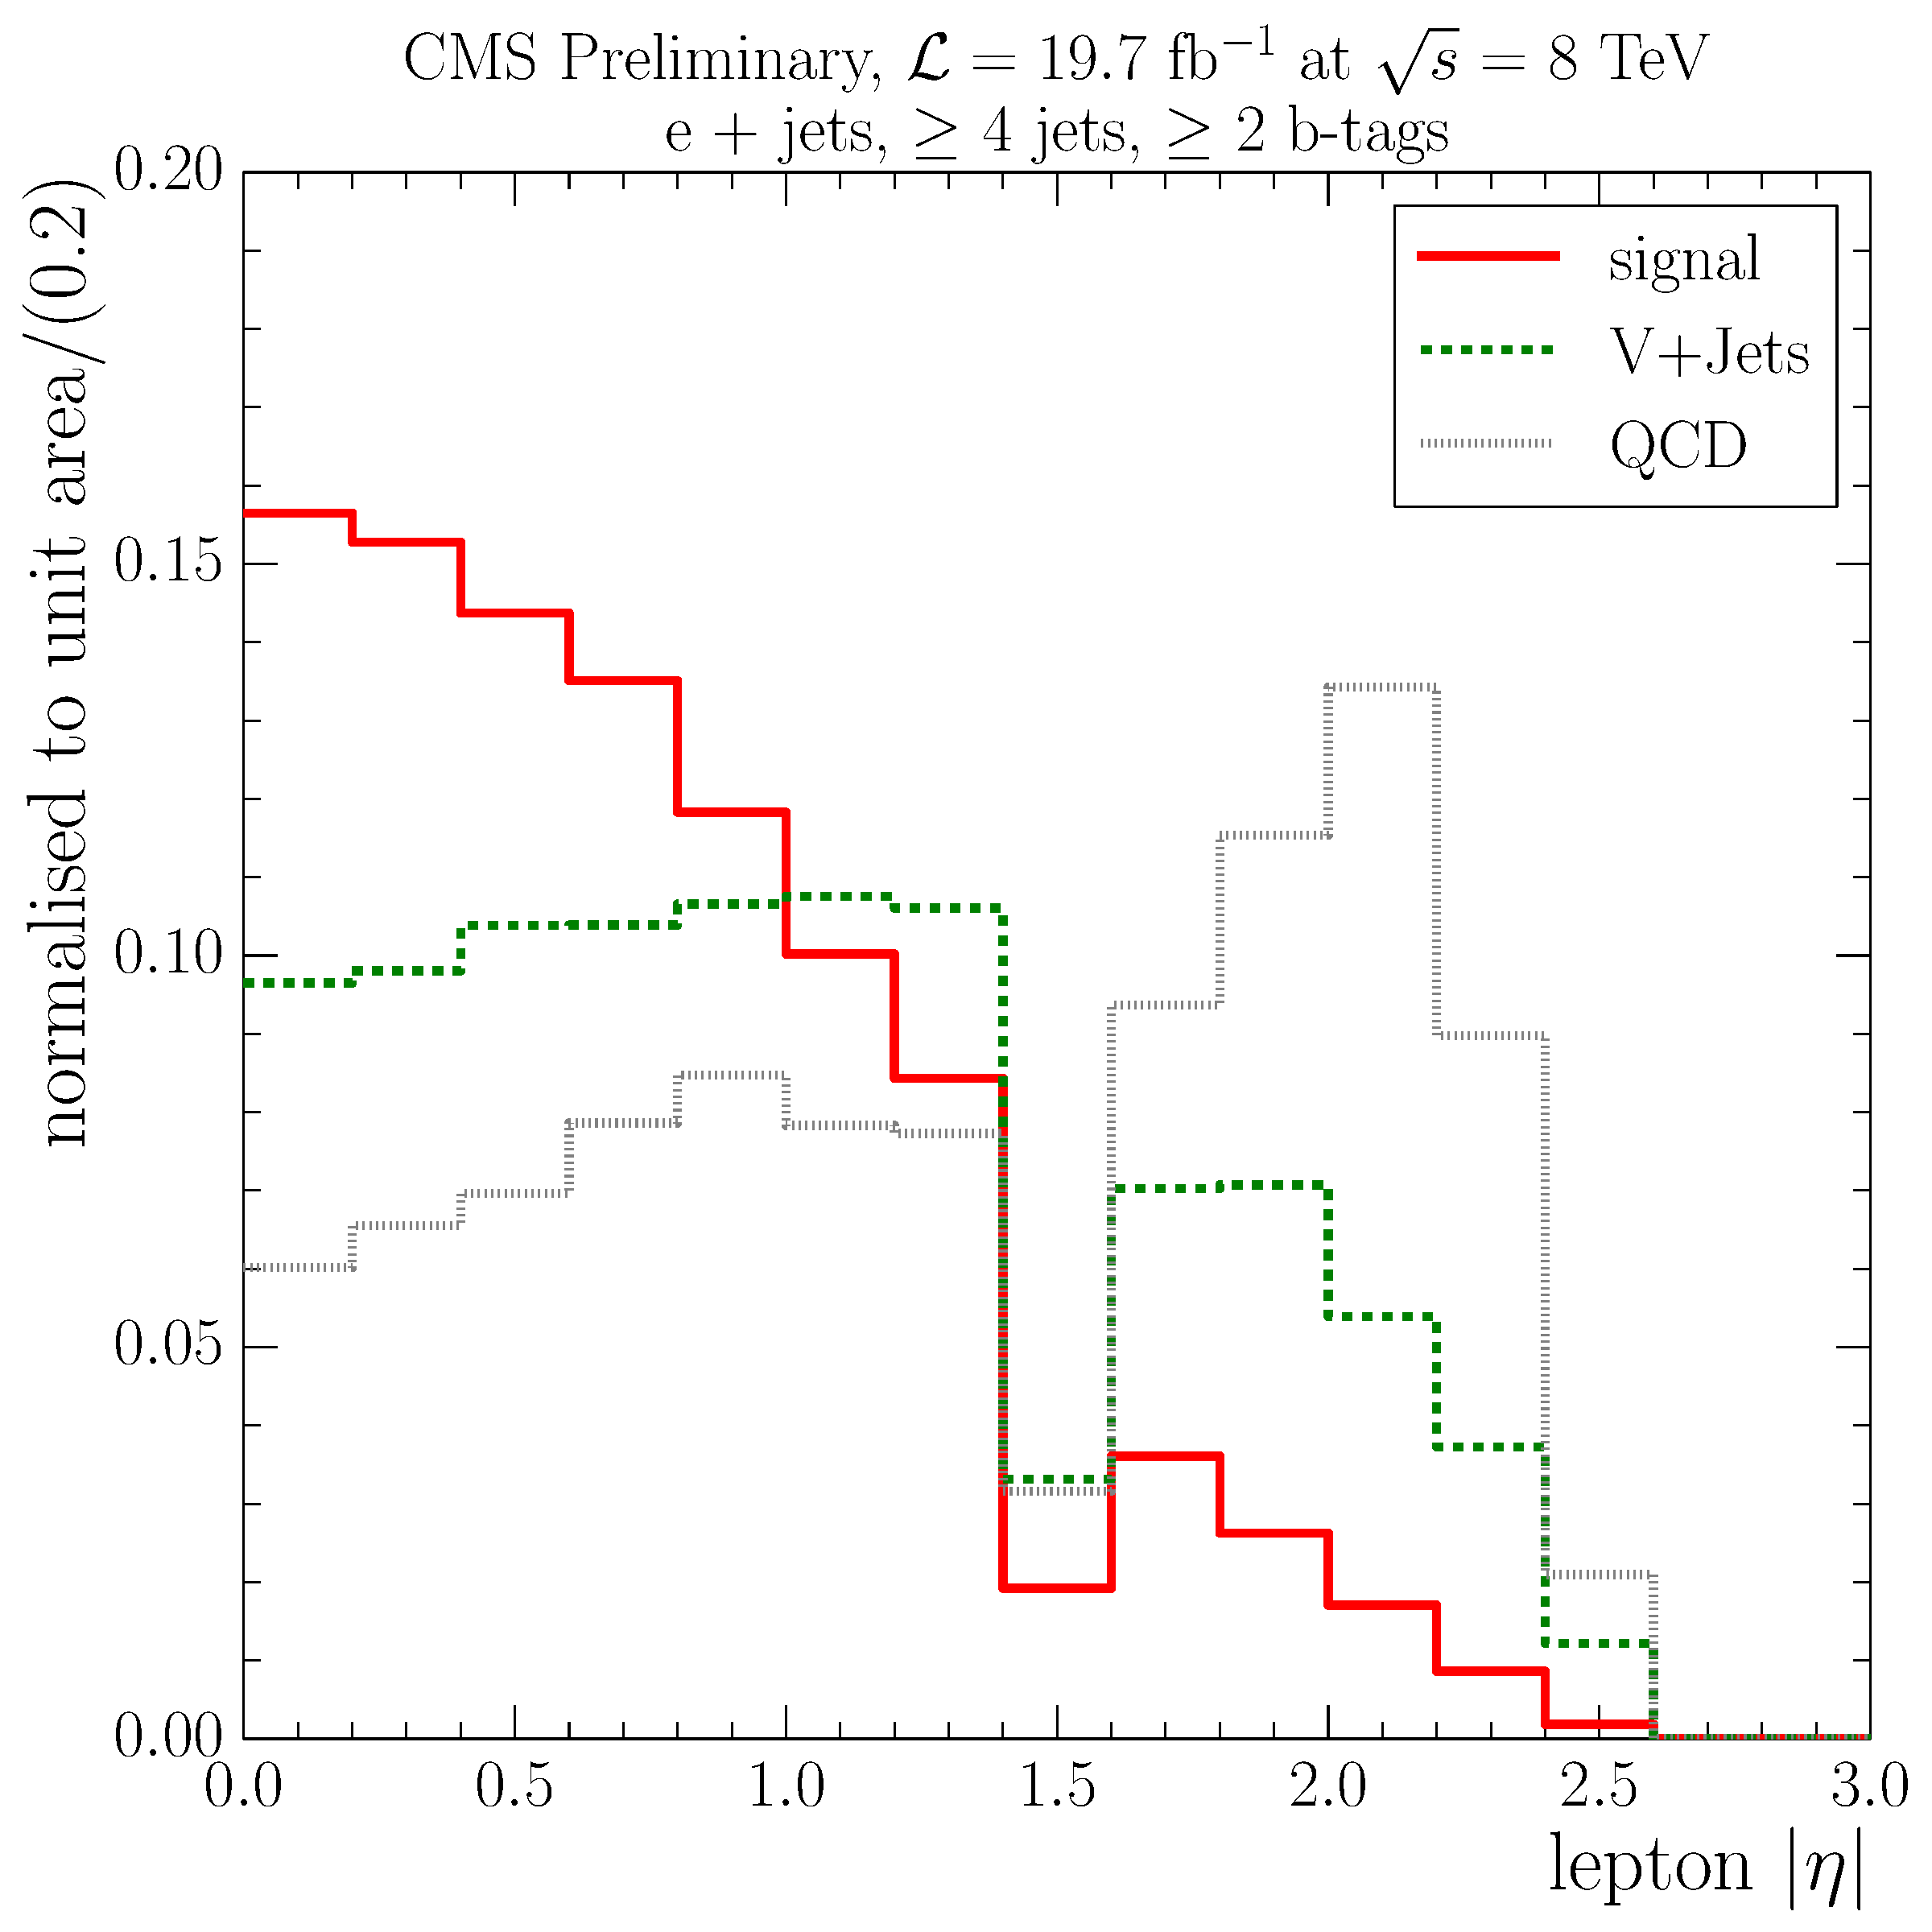
\includegraphics[width=0.42\textwidth]{measurement/MET/central/fit_templates/electron_templates_bin_70-100}}
  	\hspace*{\fill} \\
  	\hspace*{\fill}
  	{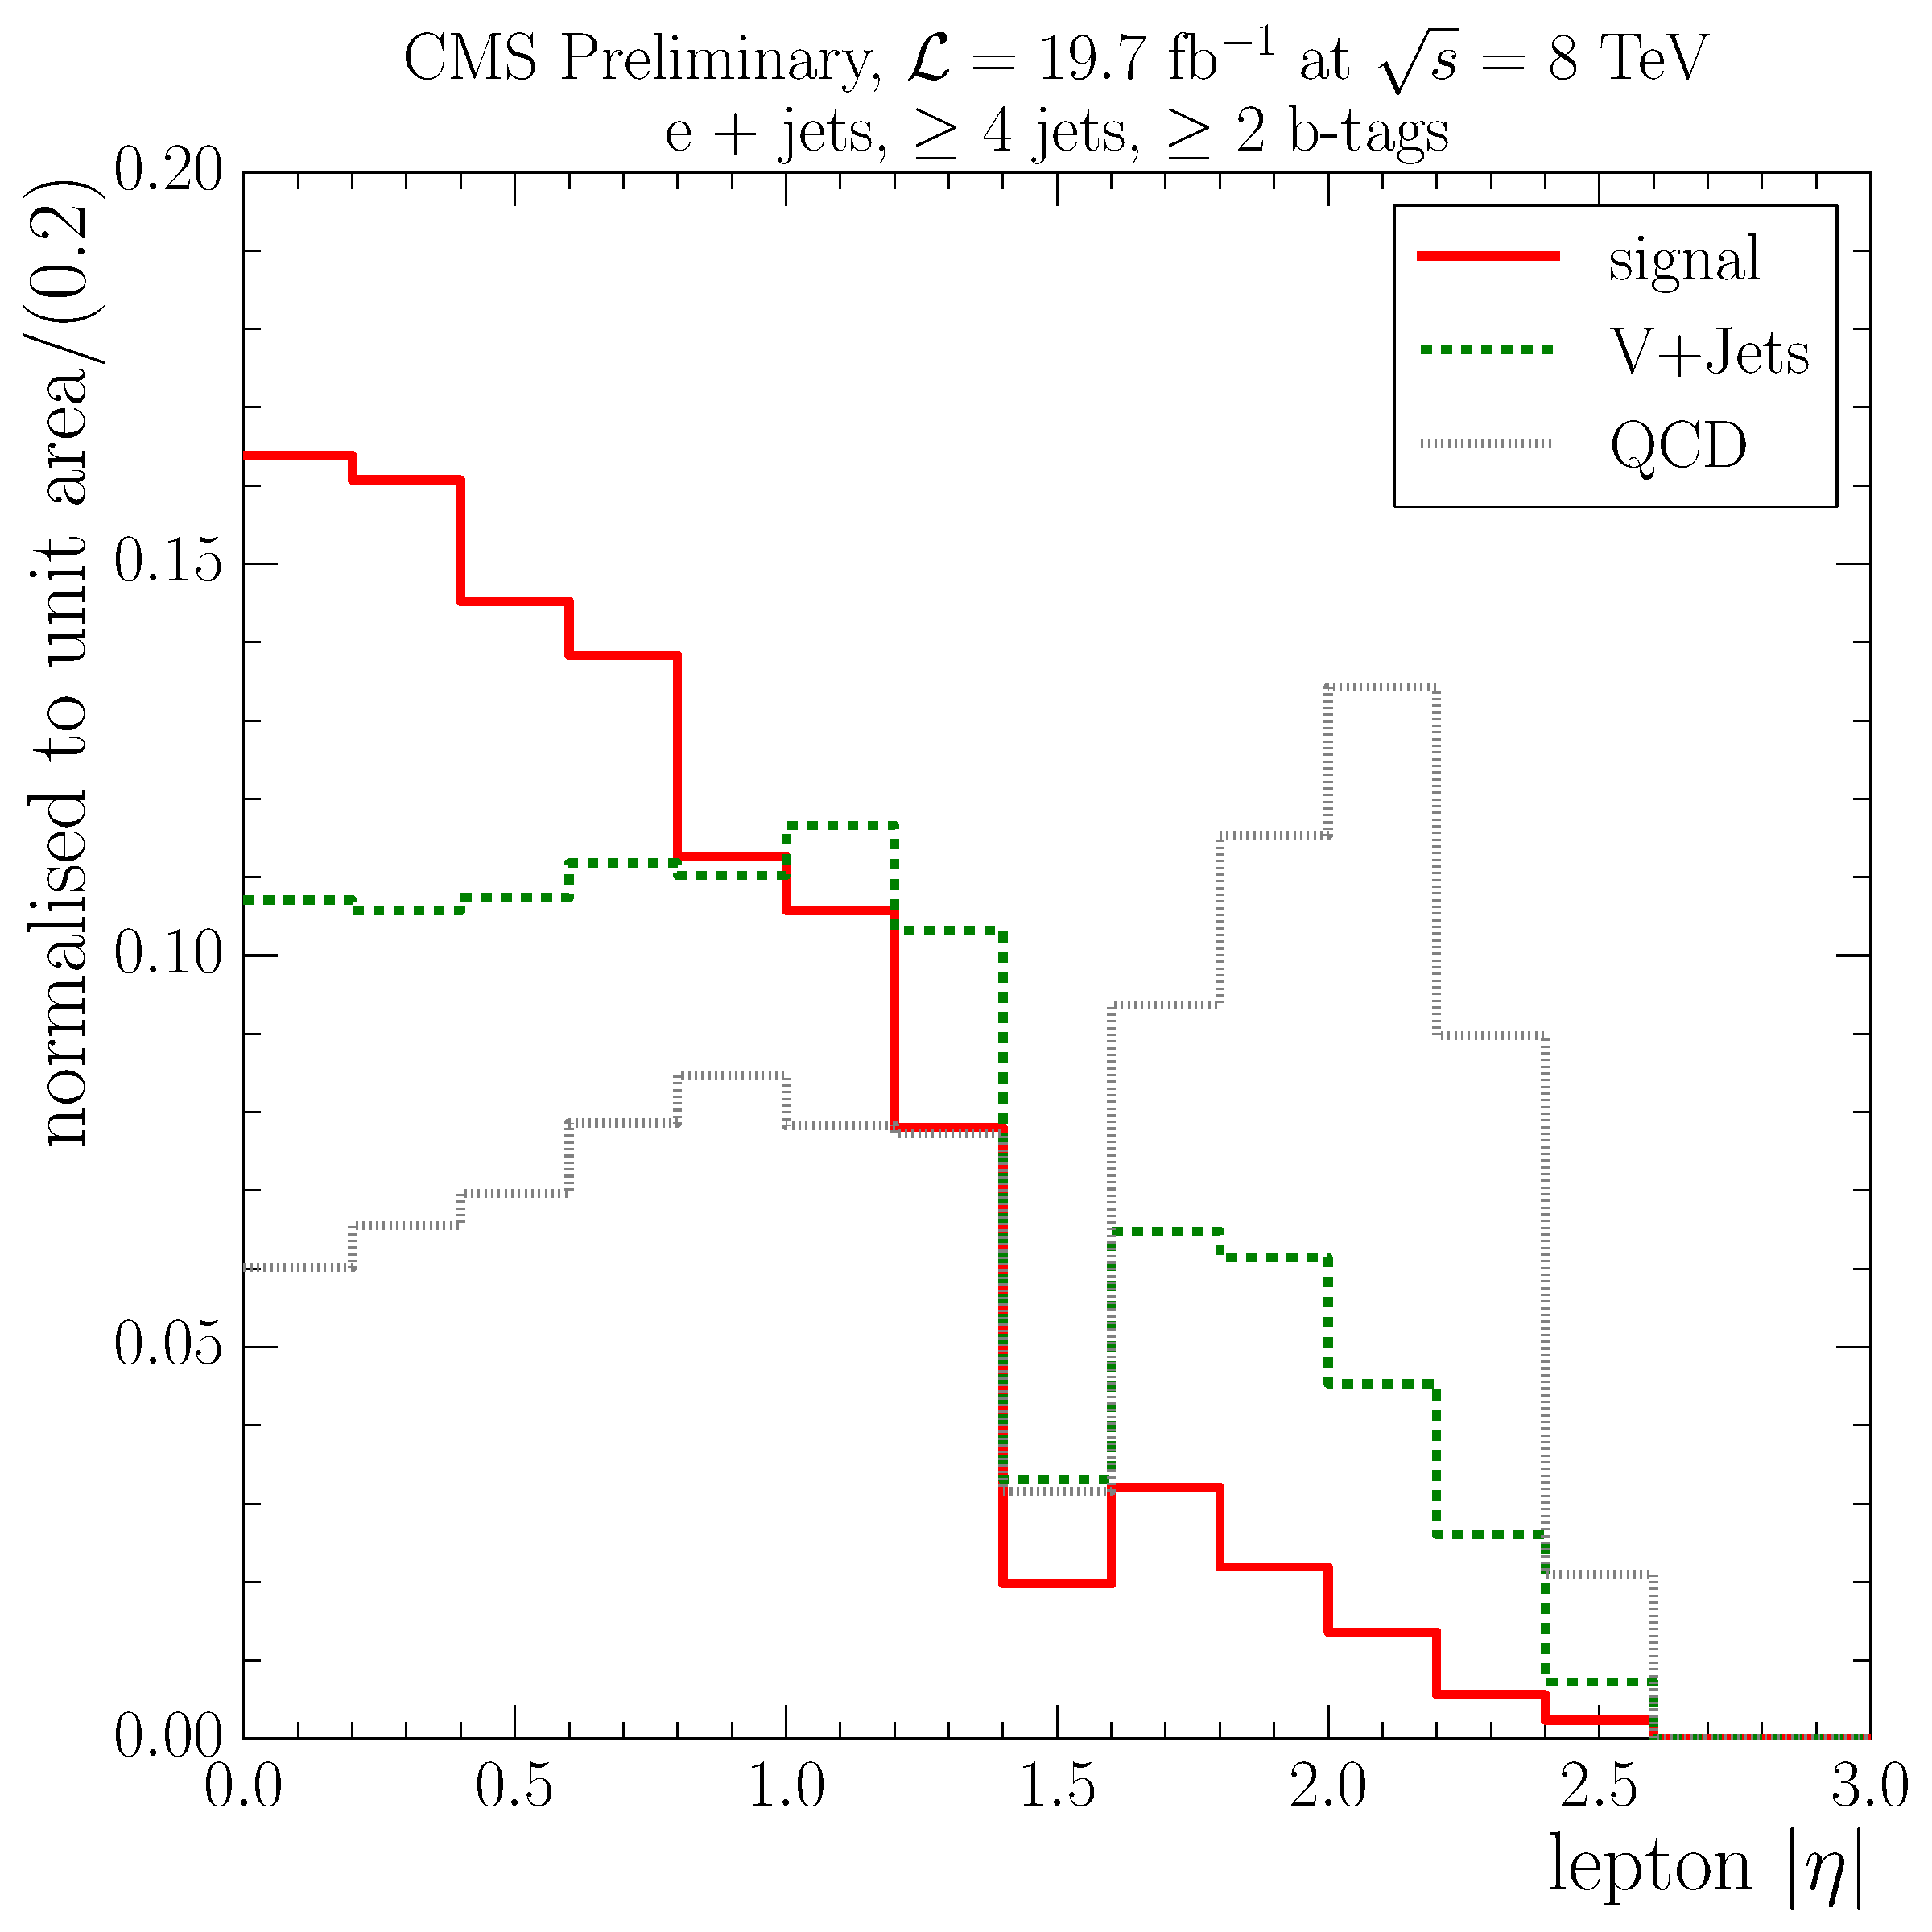
\includegraphics[width=0.42\textwidth]{measurement/MET/central/fit_templates/electron_templates_bin_100-150}}\hfill
  	{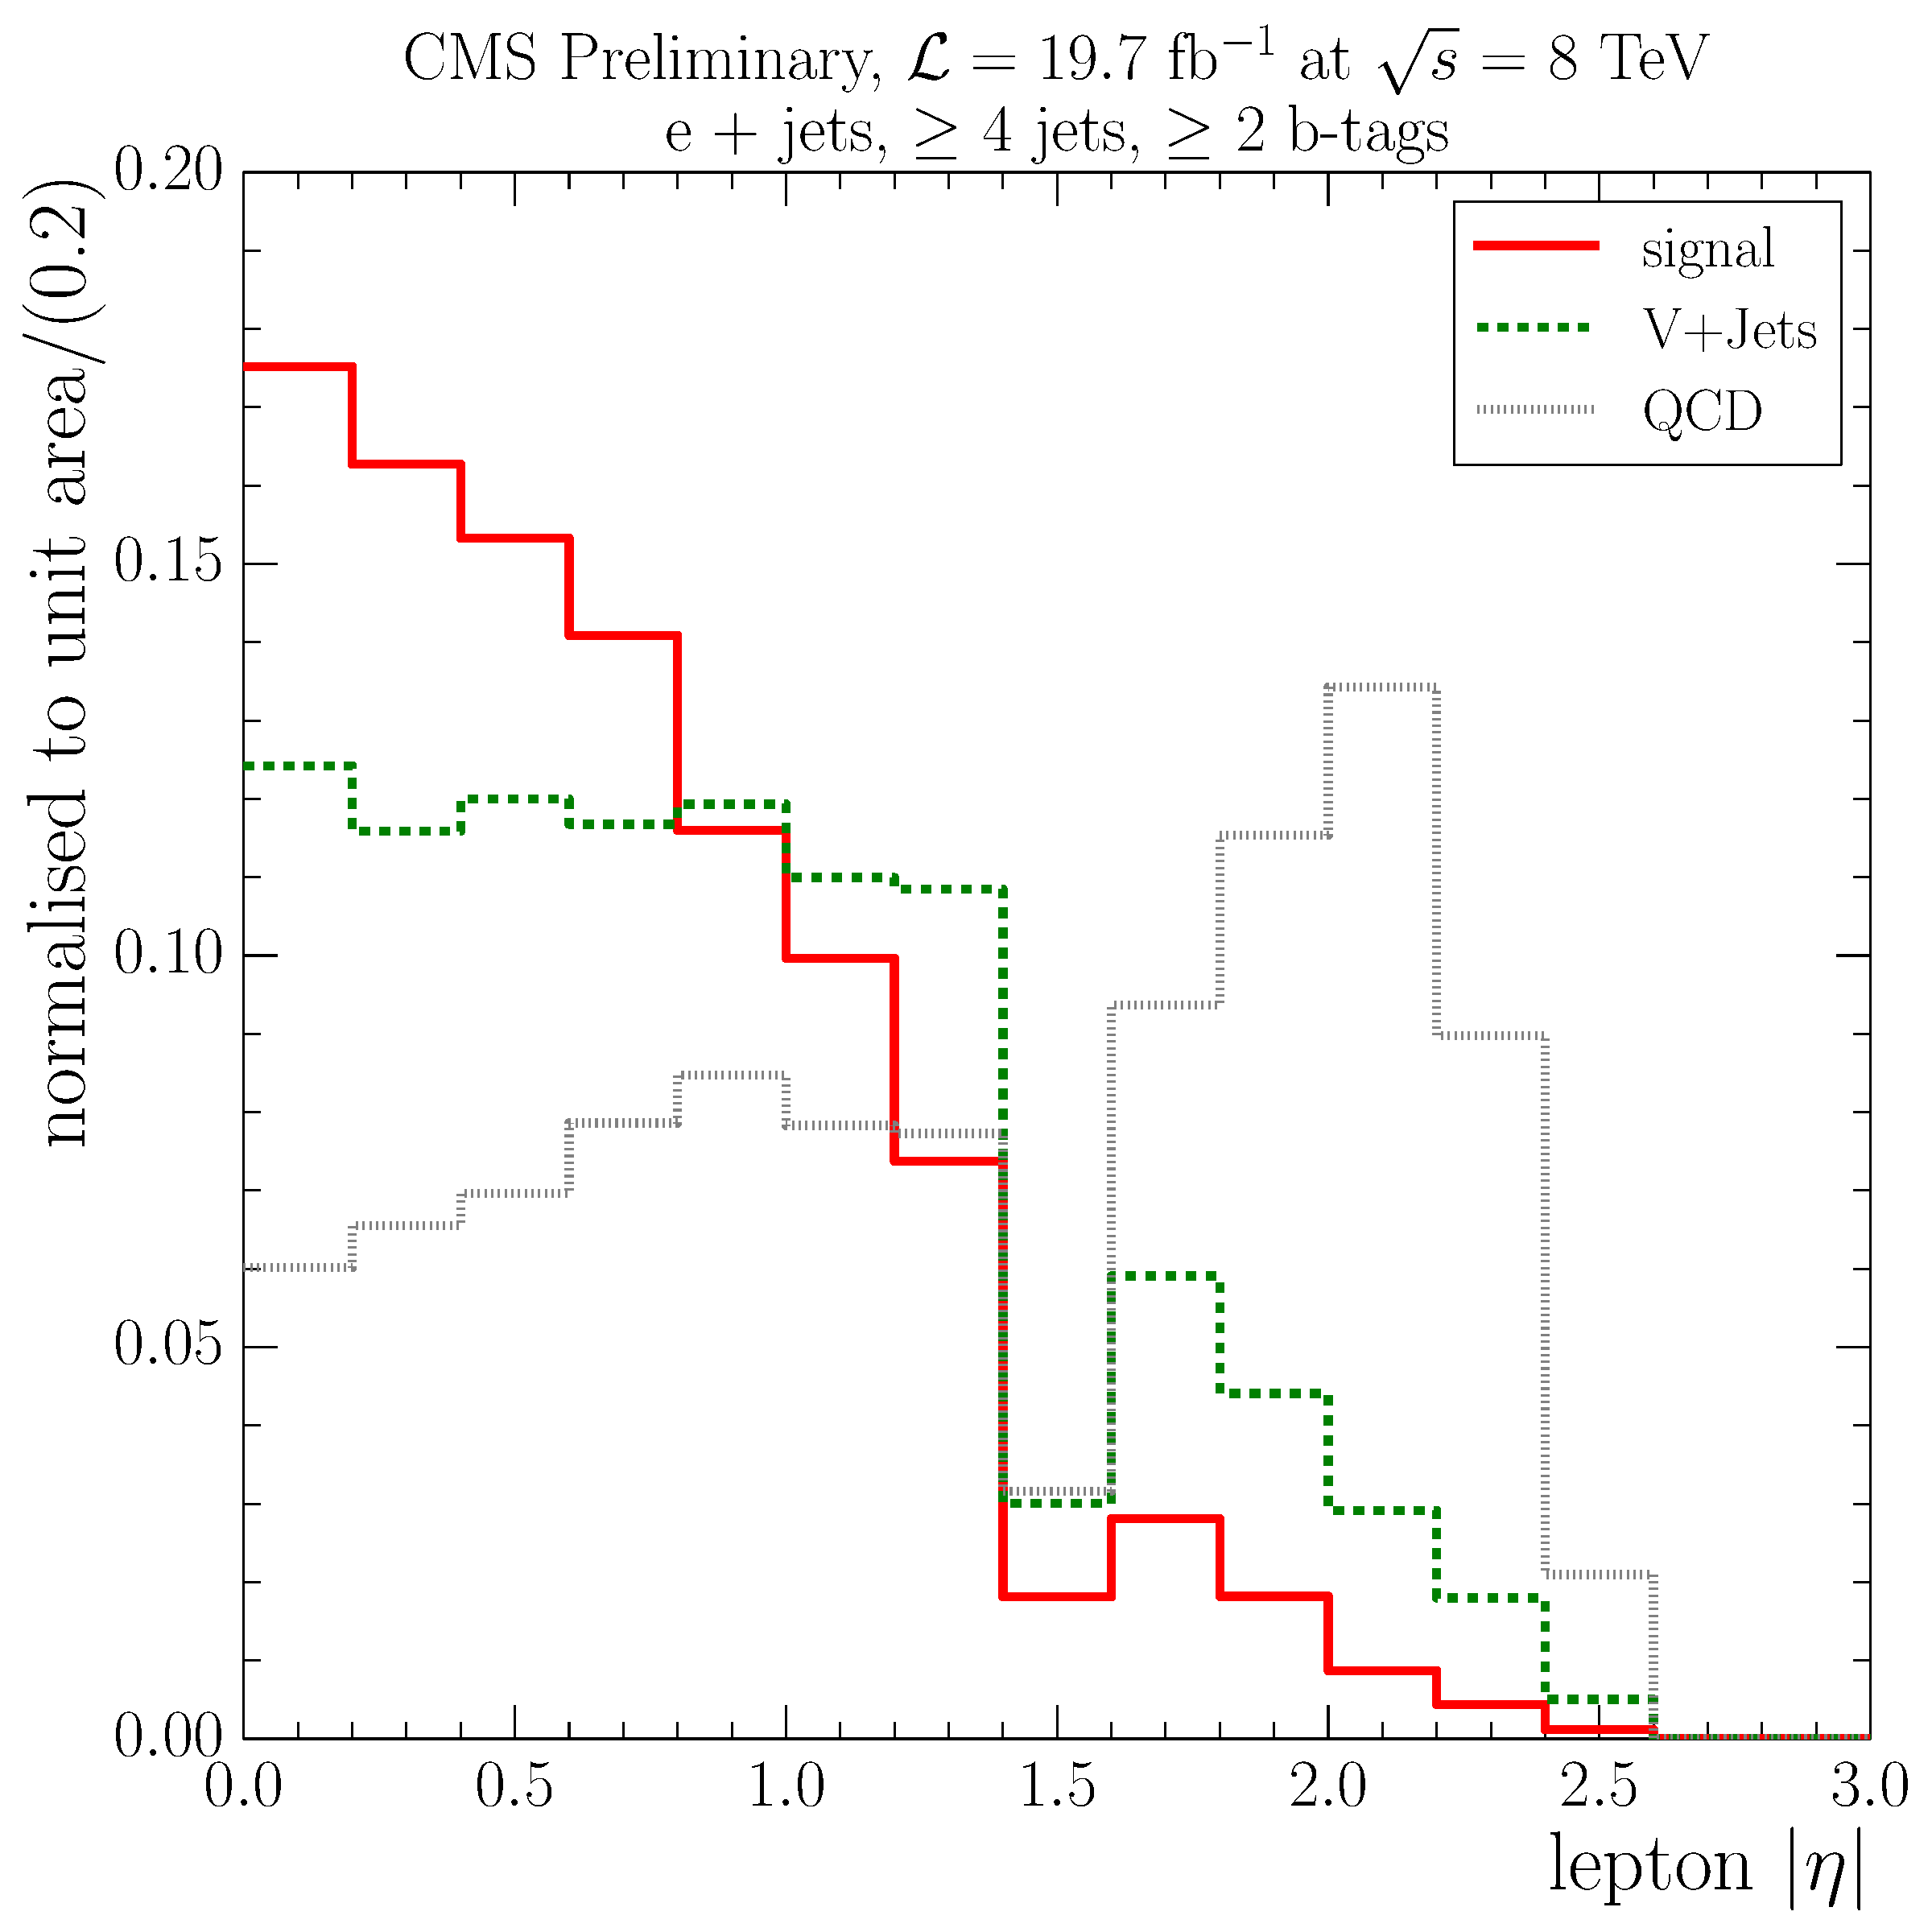
\includegraphics[width=0.42\textwidth]{measurement/MET/central/fit_templates/electron_templates_bin_150-inf}}
  	\hspace*{\fill}
    \caption[Electron $\abs \eta$ templates for the fit in different bins of \MET]{Electron $\abs \eta$ templates for
    the fit in different bins of \MET, from top left to bottom right: \SIrange{0}{25}{\GeV}, \SIrange{25}{45}{\GeV},
    \SIrange{45}{70}{\GeV}, \SIrange{70}{100}{\GeV}, \SIrange{100}{150}{\GeV} and $\geq \SI{150}{\GeV}$.}
    \label{fig:fit_templates_MET_electron}
\end{figure}

\begin{figure}[!htbp]
	\centering
	\vspace*{-0.5cm}
	\hspace*{\fill}
  	{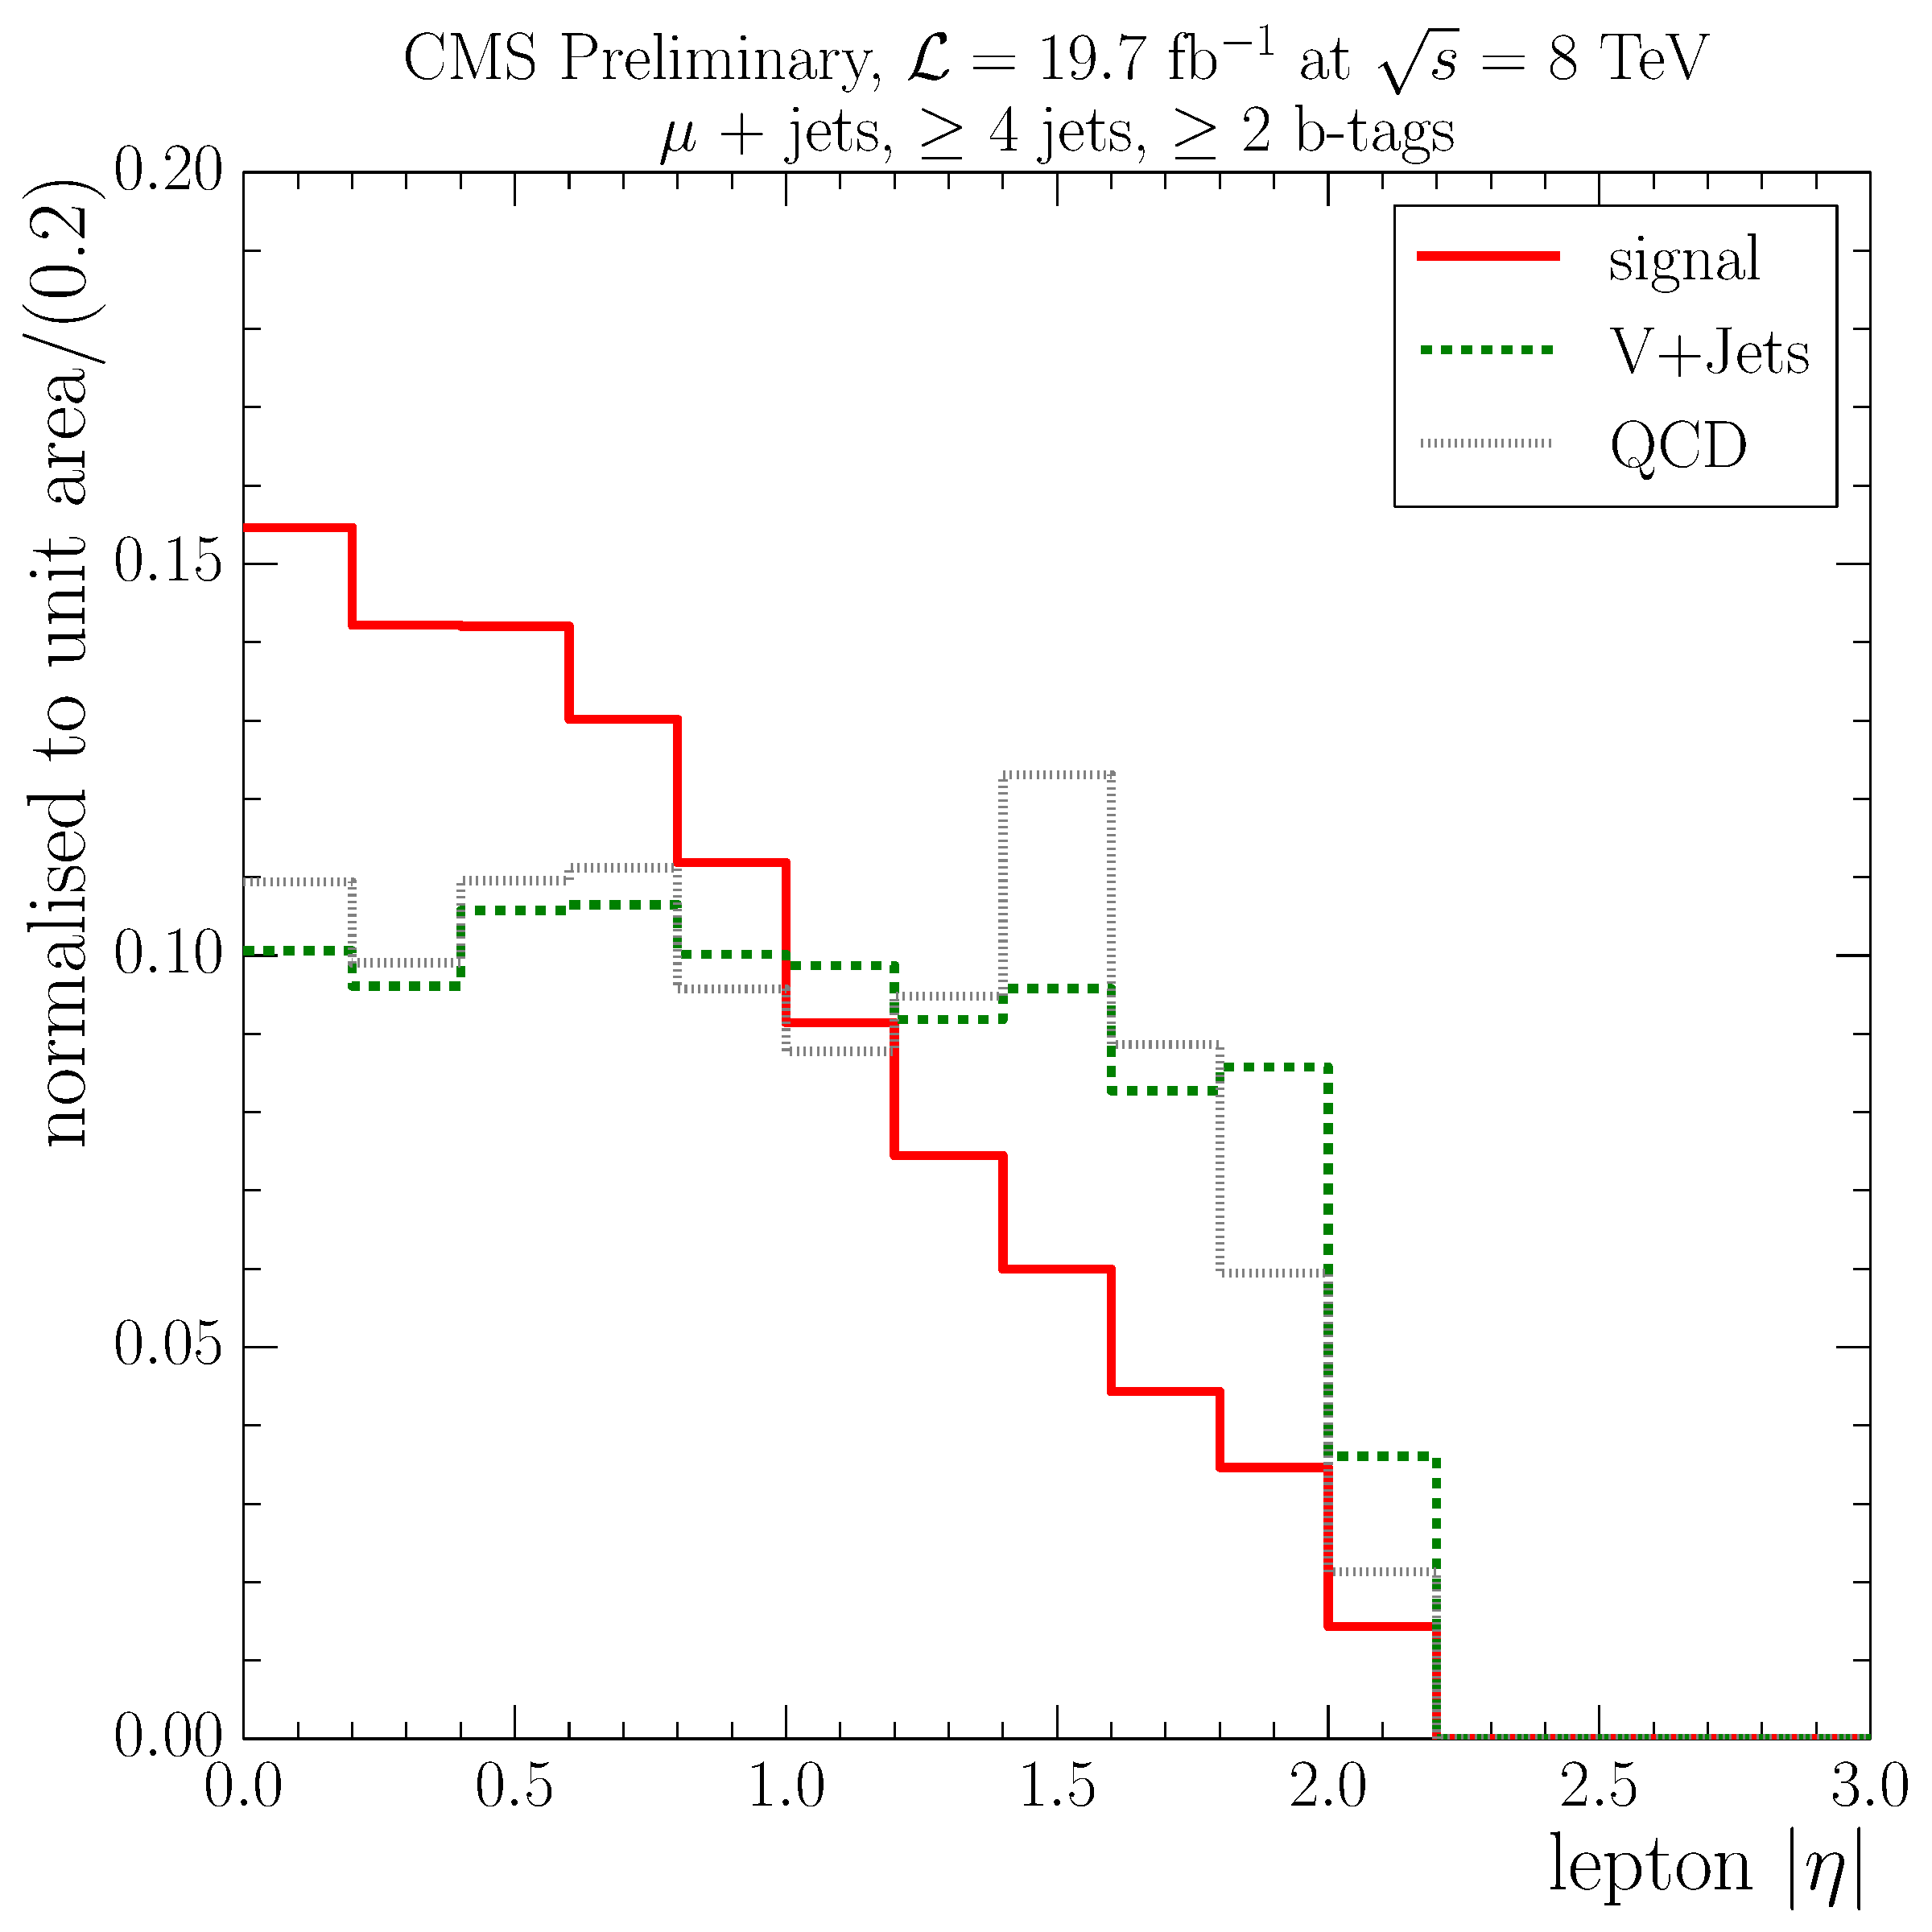
\includegraphics[width=0.42\textwidth]{measurement/MET/central/fit_templates/muon_templates_bin_0-25}}\hfill
  	{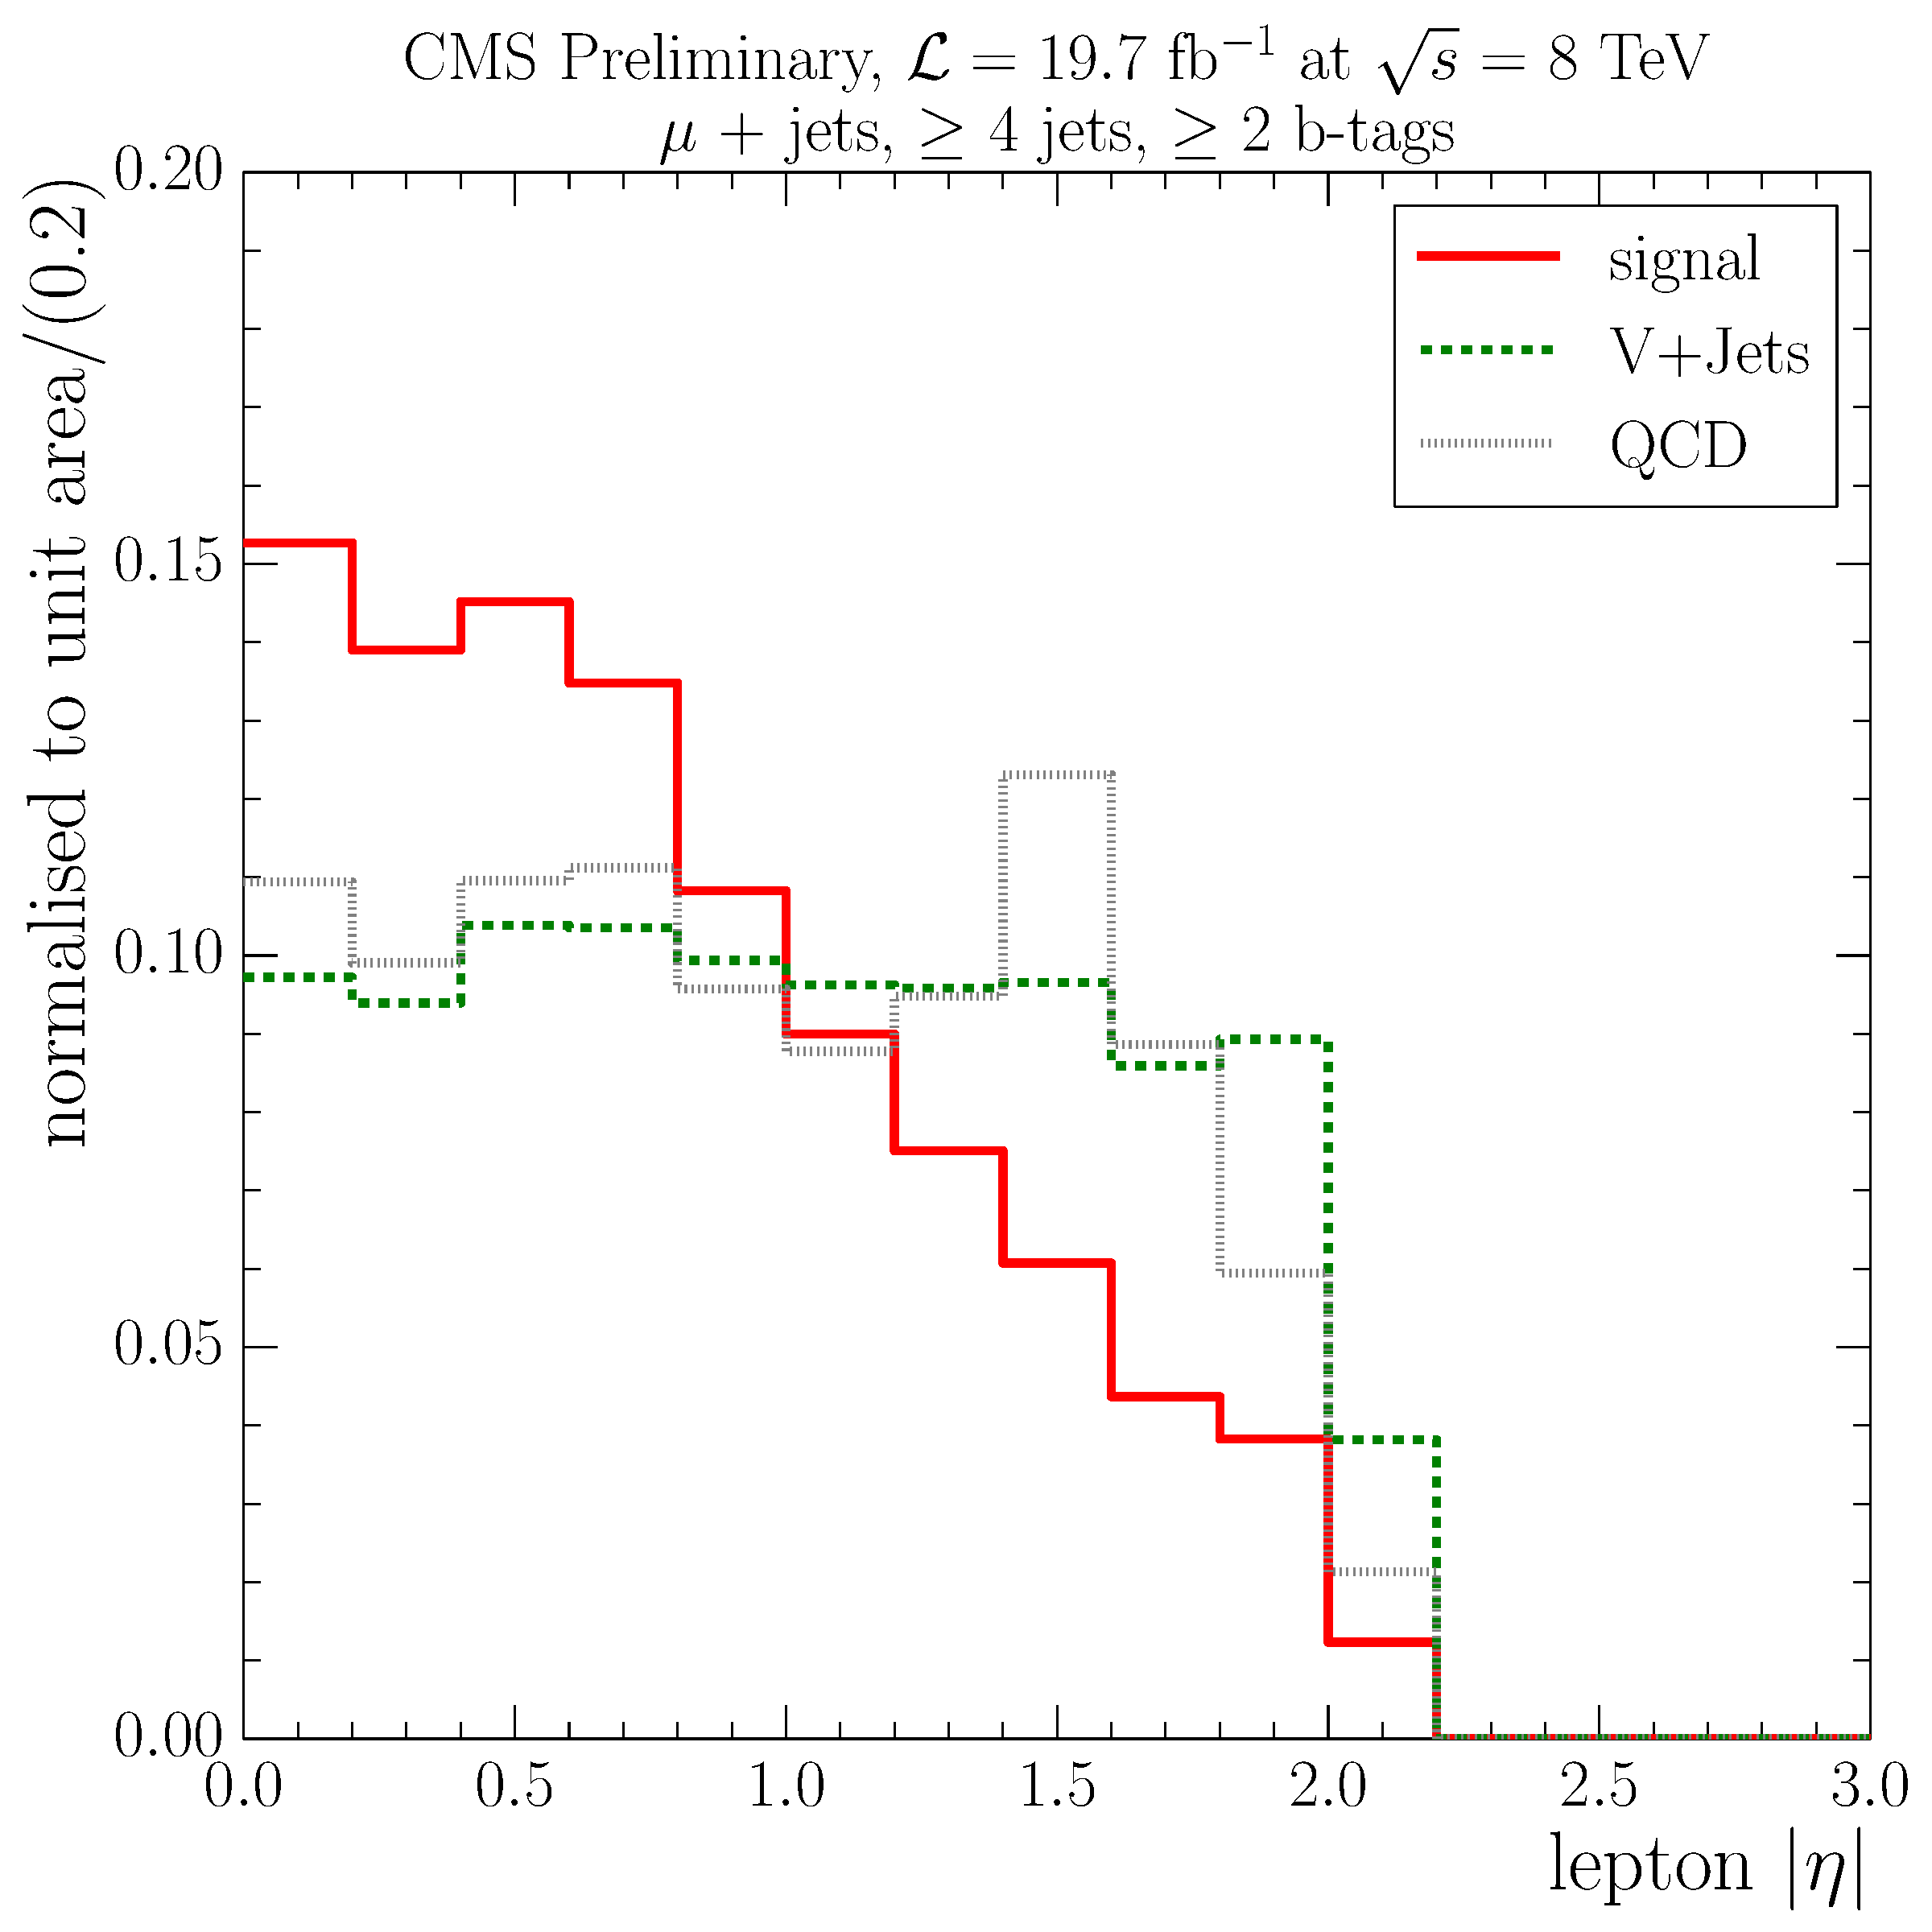
\includegraphics[width=0.42\textwidth]{measurement/MET/central/fit_templates/muon_templates_bin_25-45}}
  	\hspace*{\fill} \\
  	\hspace*{\fill}
  	{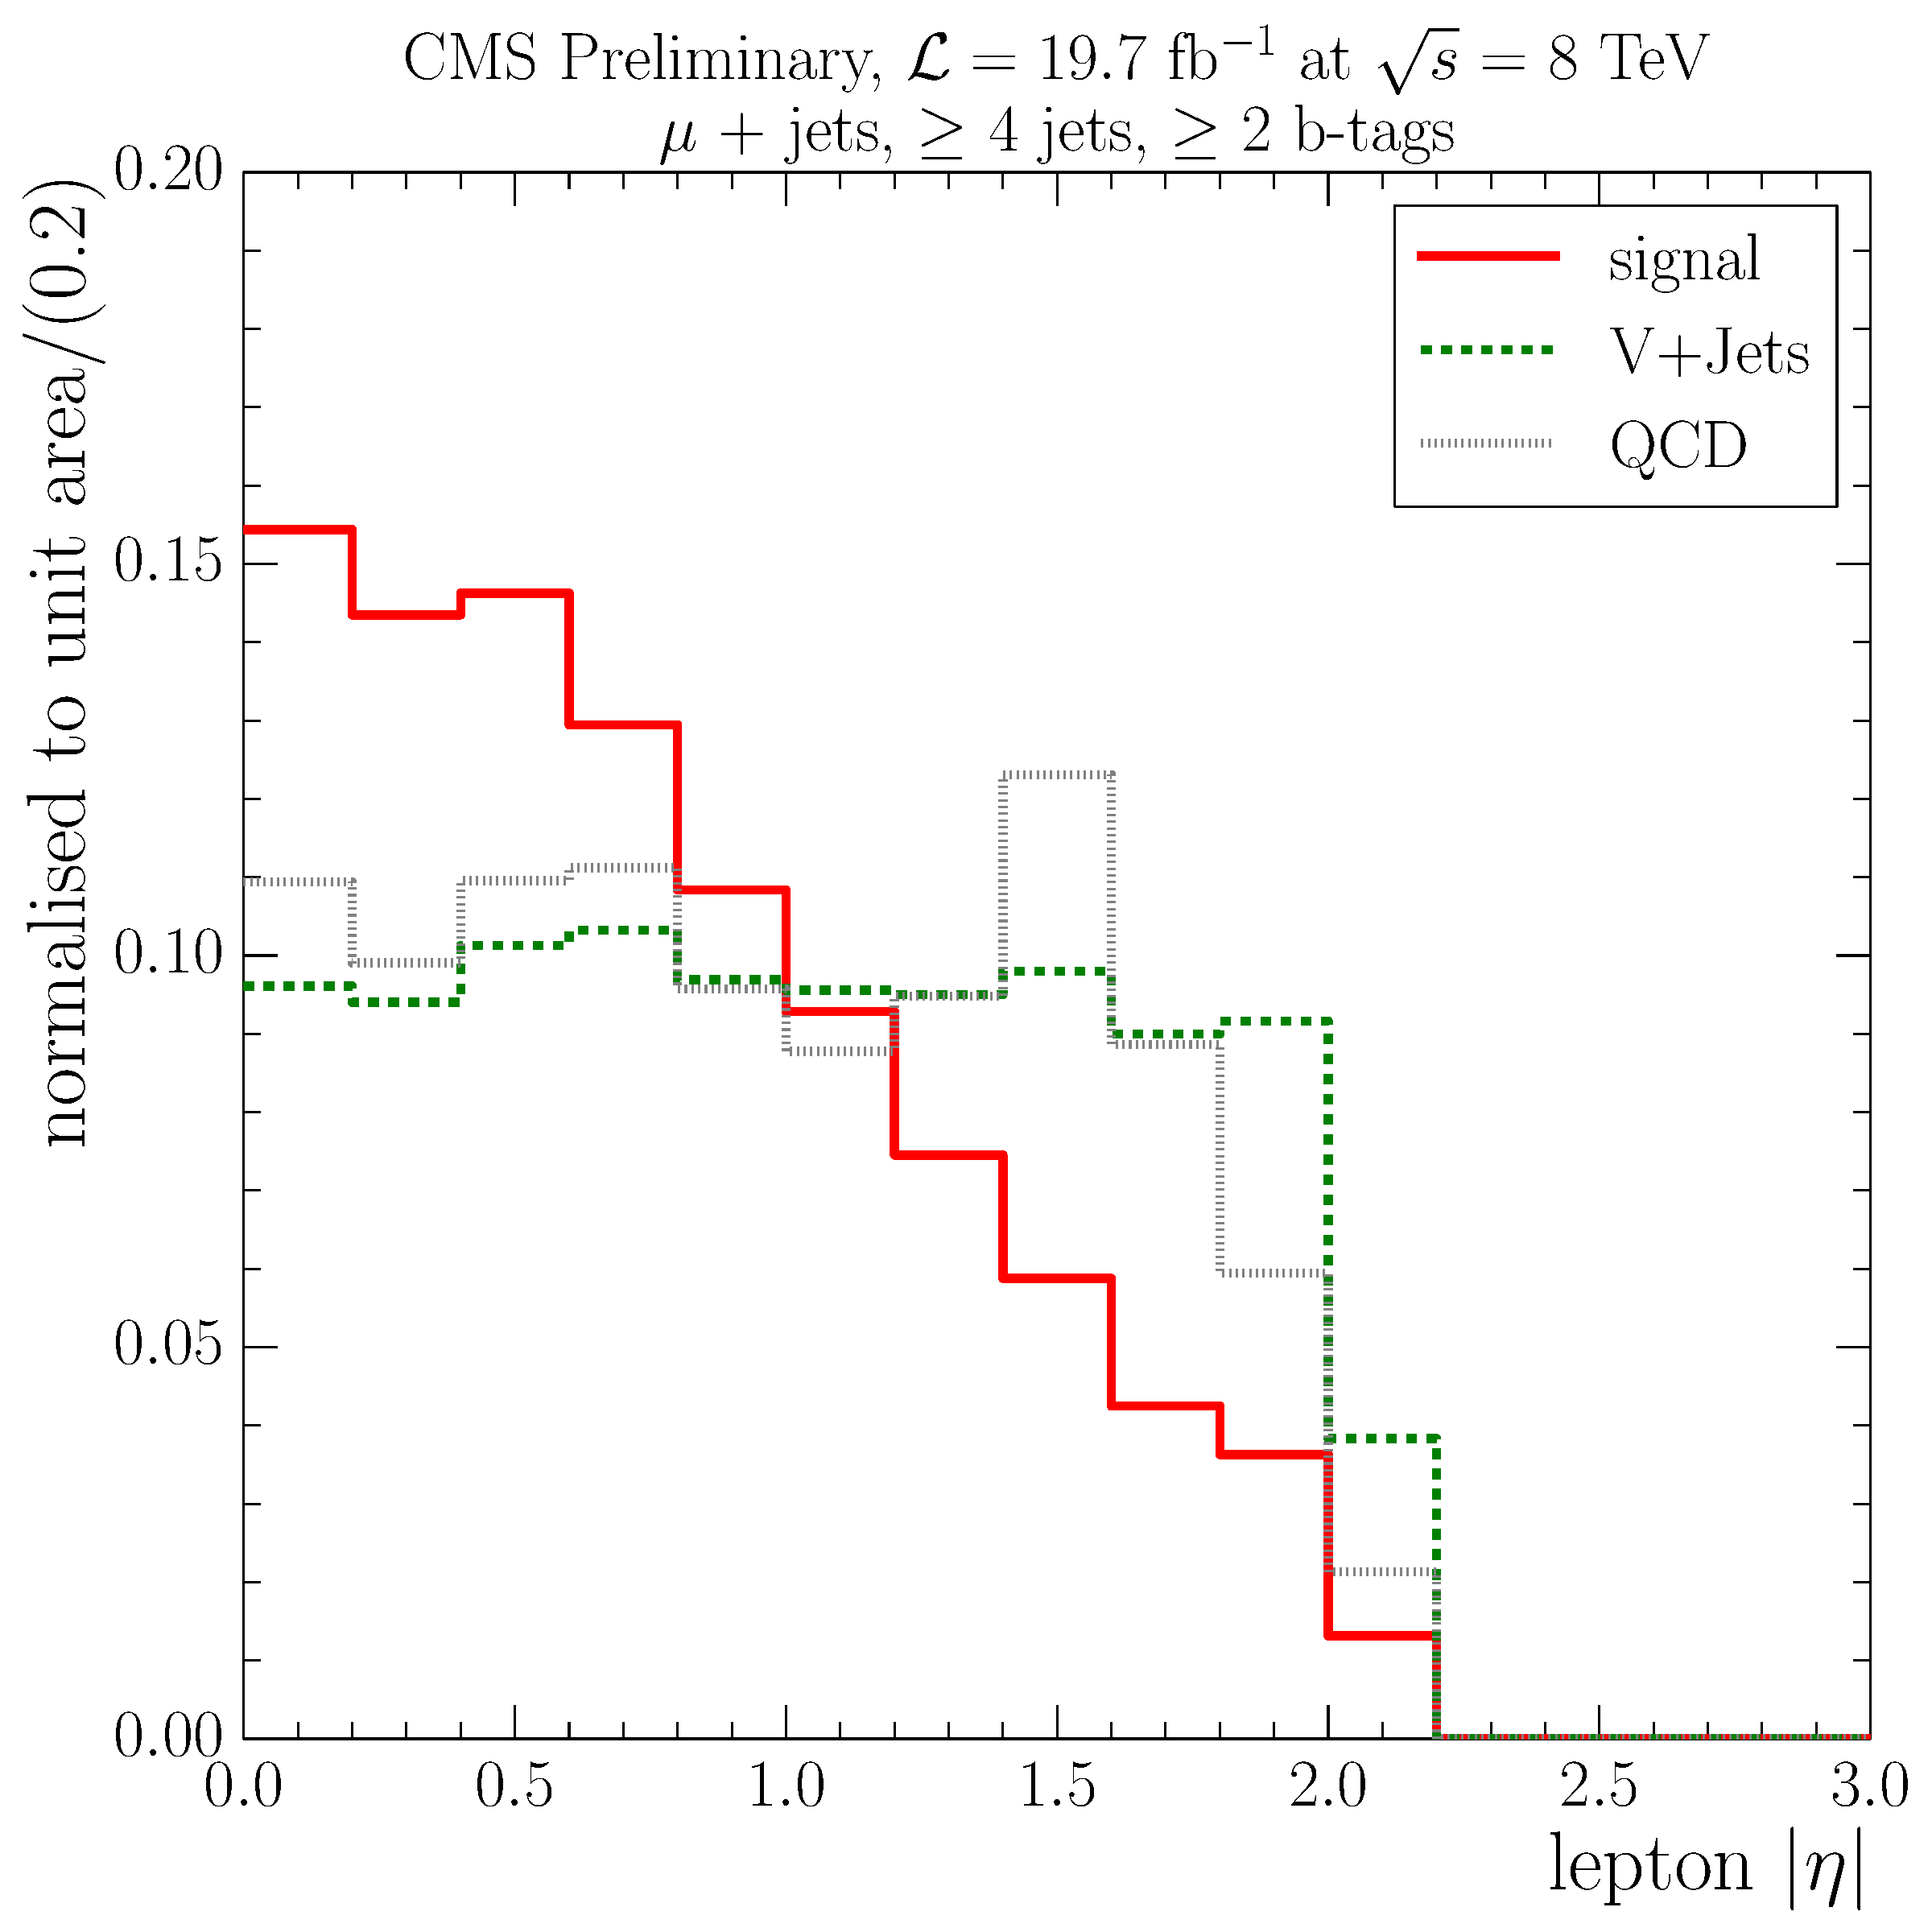
\includegraphics[width=0.42\textwidth]{measurement/MET/central/fit_templates/muon_templates_bin_45-70}}\hfill
  	{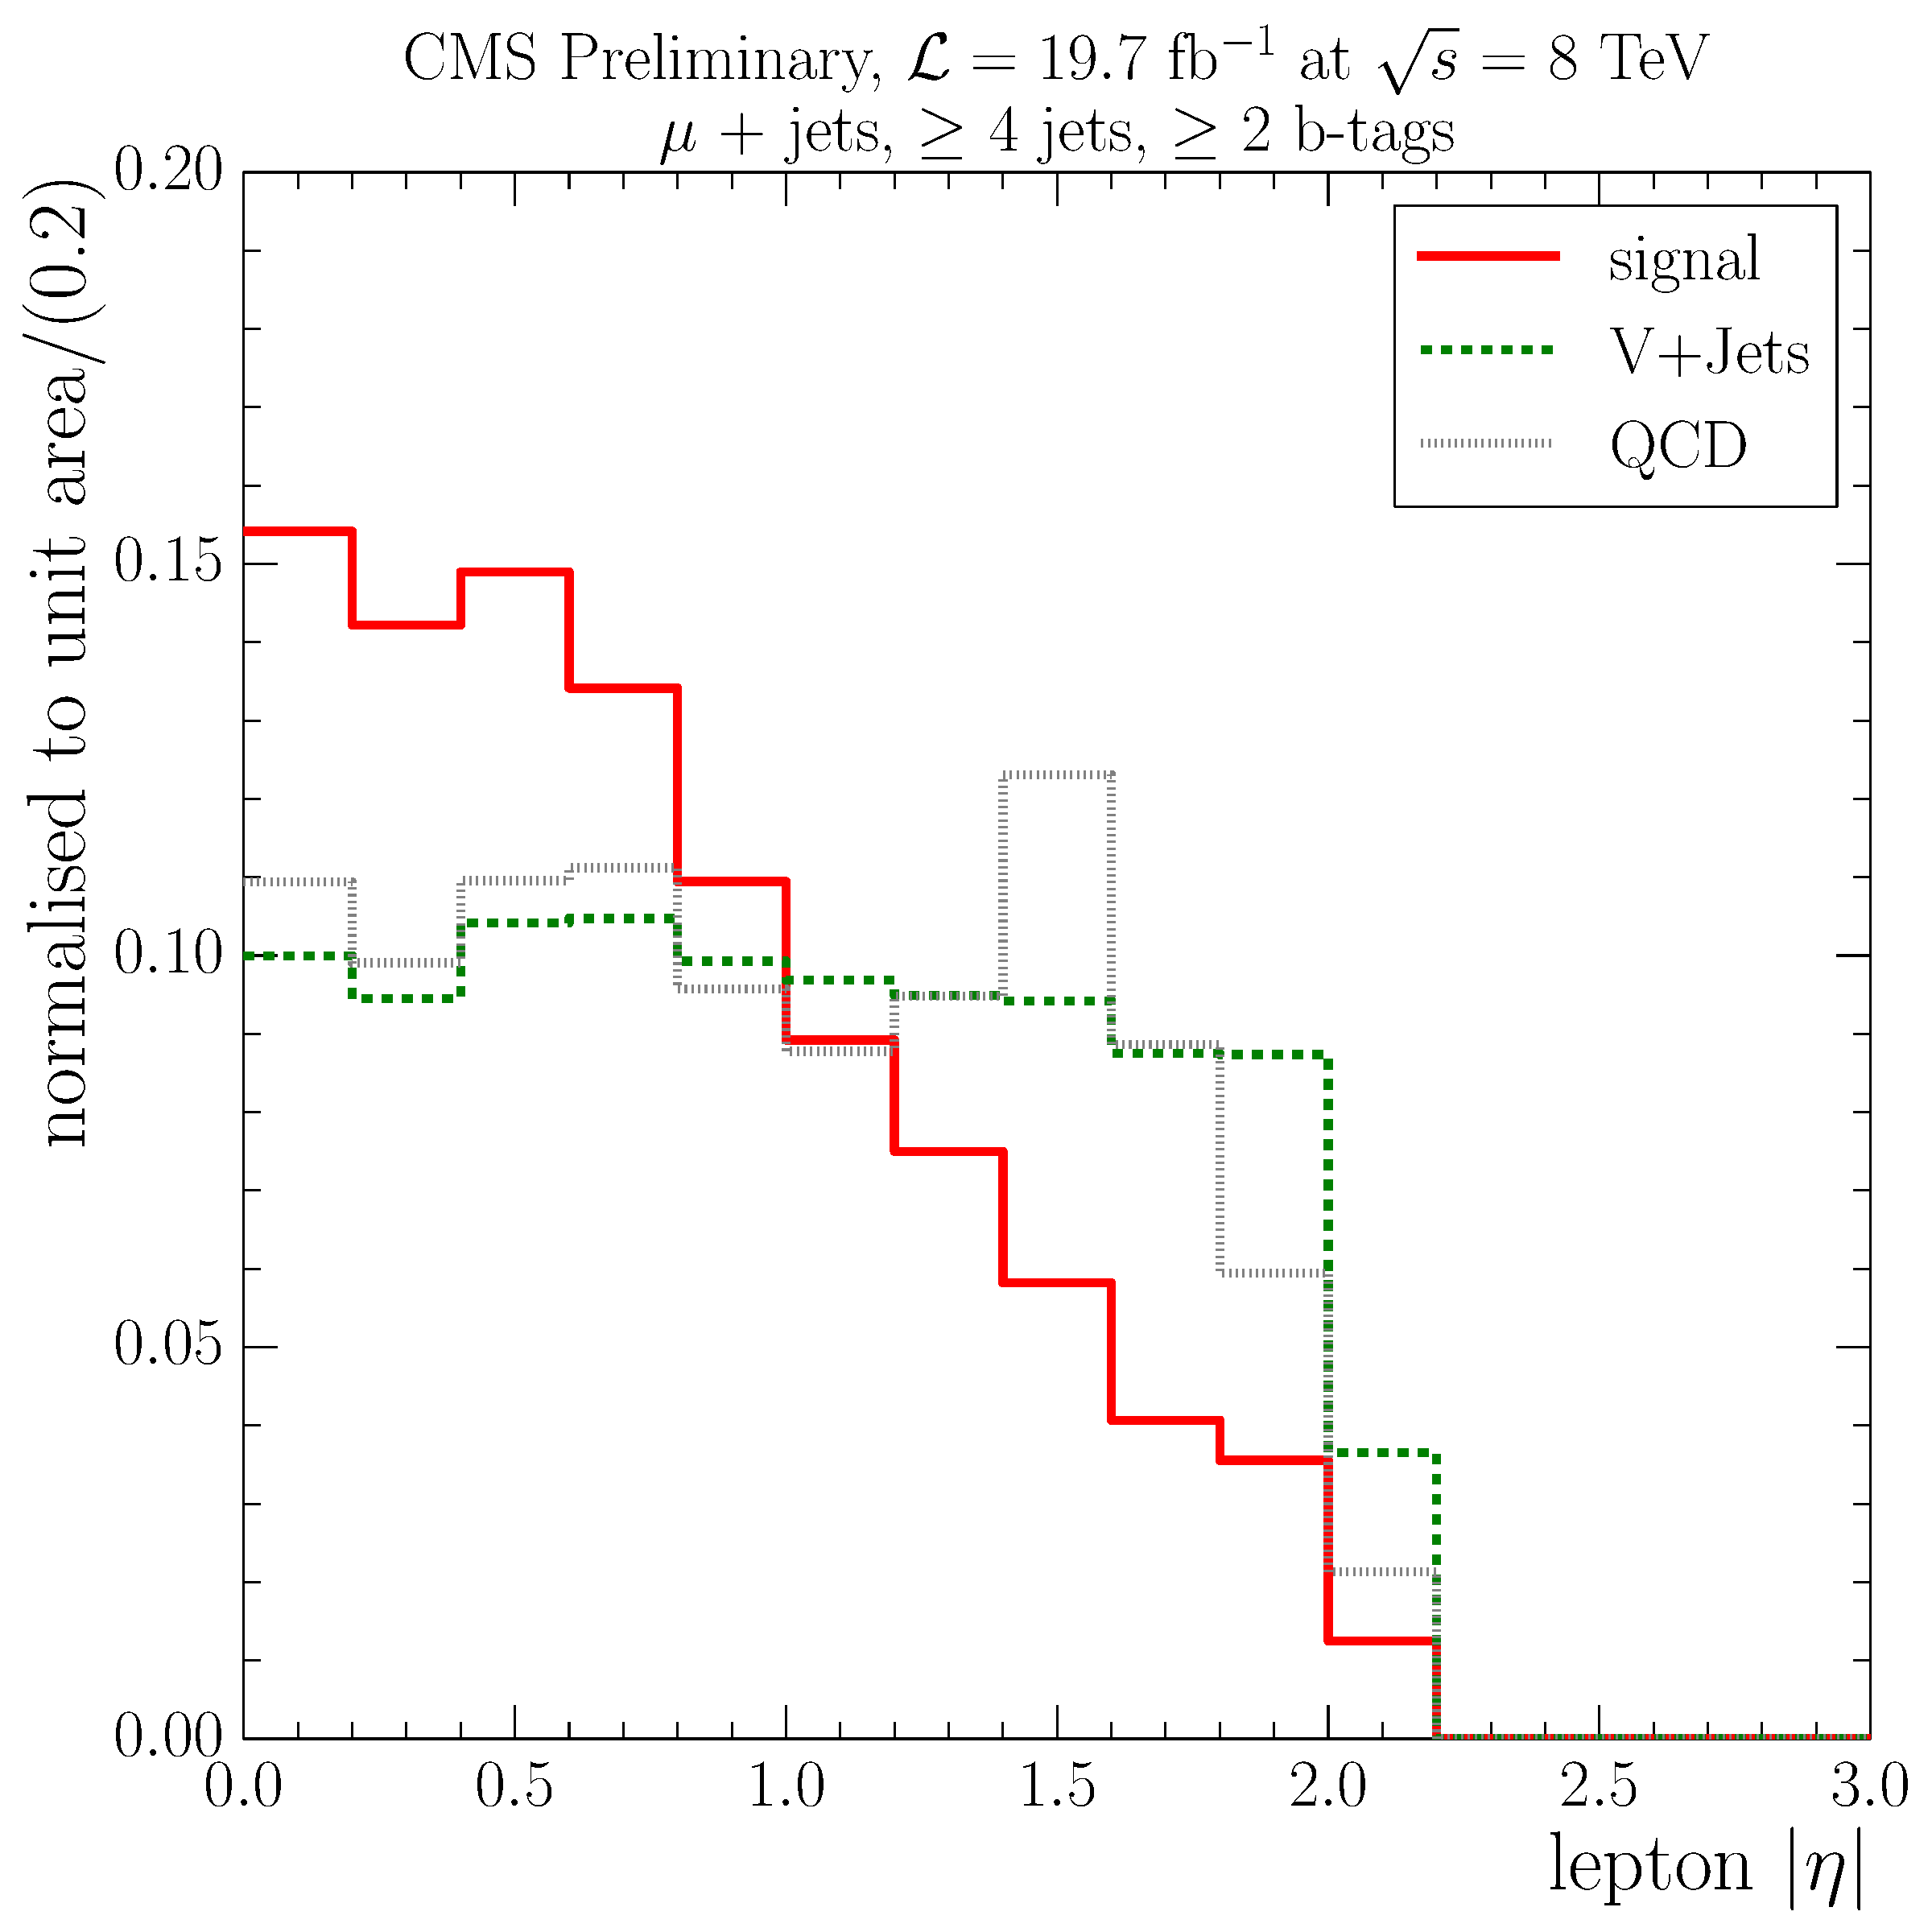
\includegraphics[width=0.42\textwidth]{measurement/MET/central/fit_templates/muon_templates_bin_70-100}}
  	\hspace*{\fill} \\
  	\hspace*{\fill}
  	{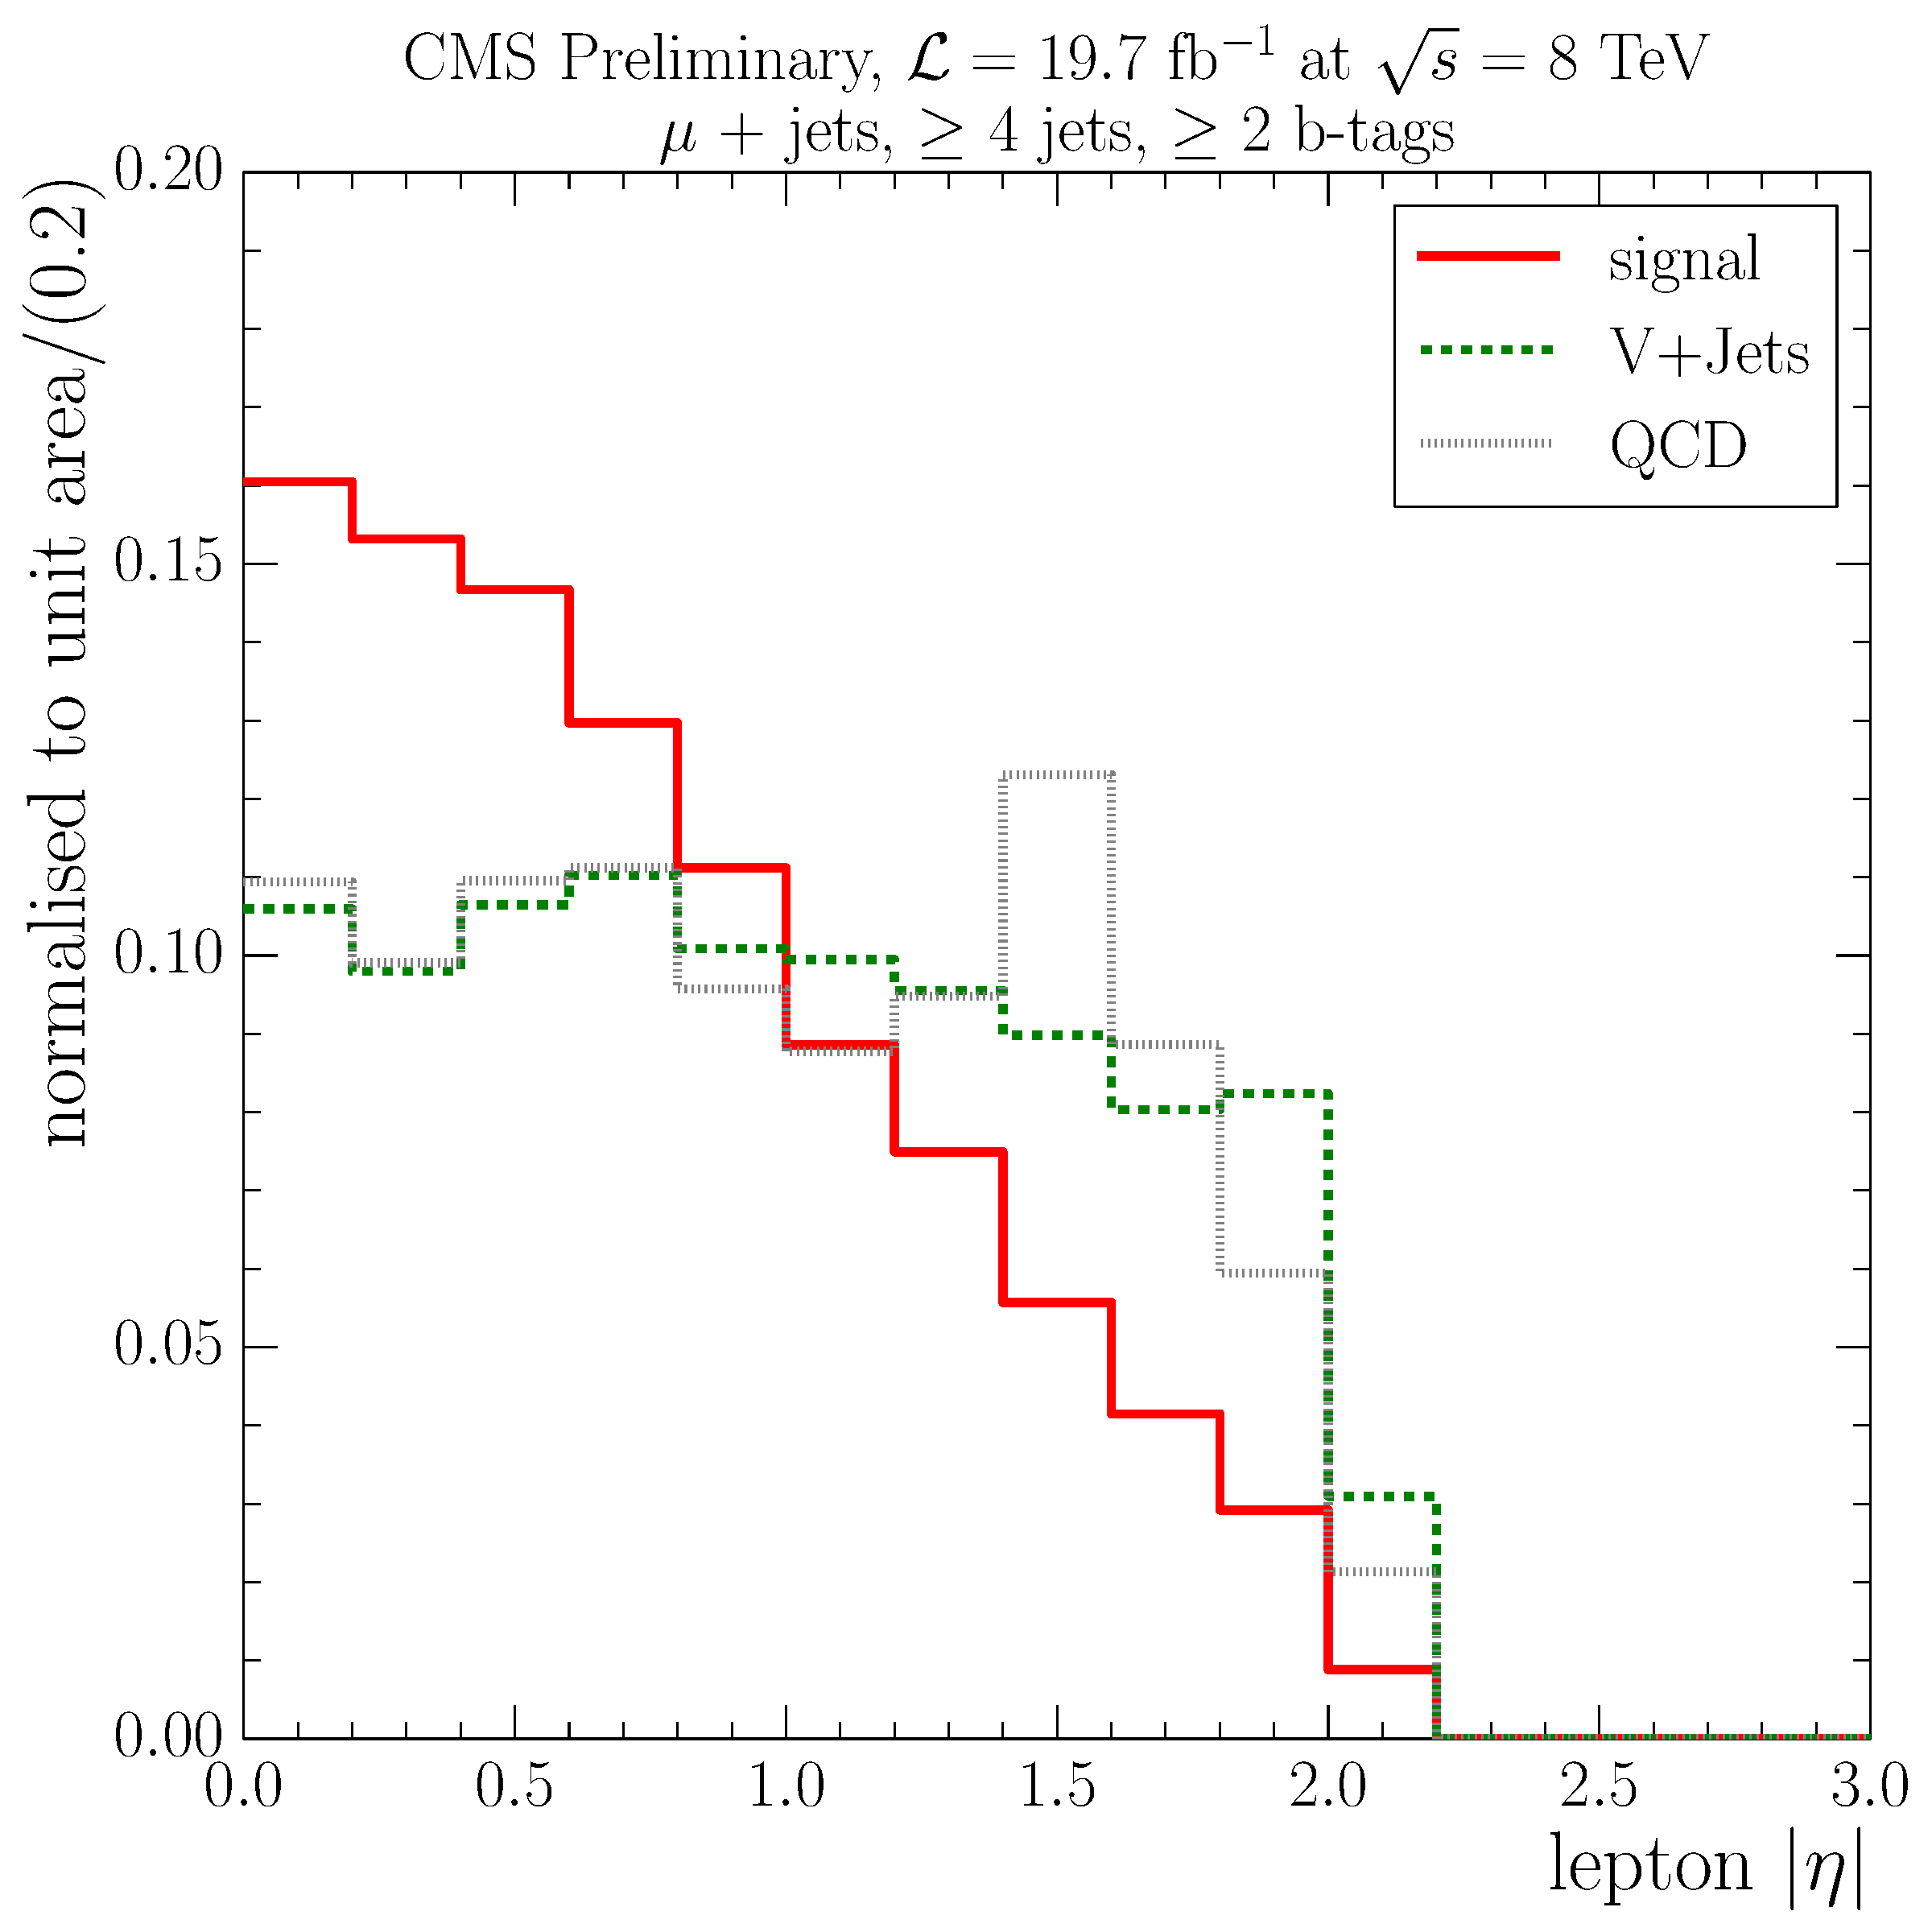
\includegraphics[width=0.42\textwidth]{measurement/MET/central/fit_templates/muon_templates_bin_100-150}}\hfill
  	{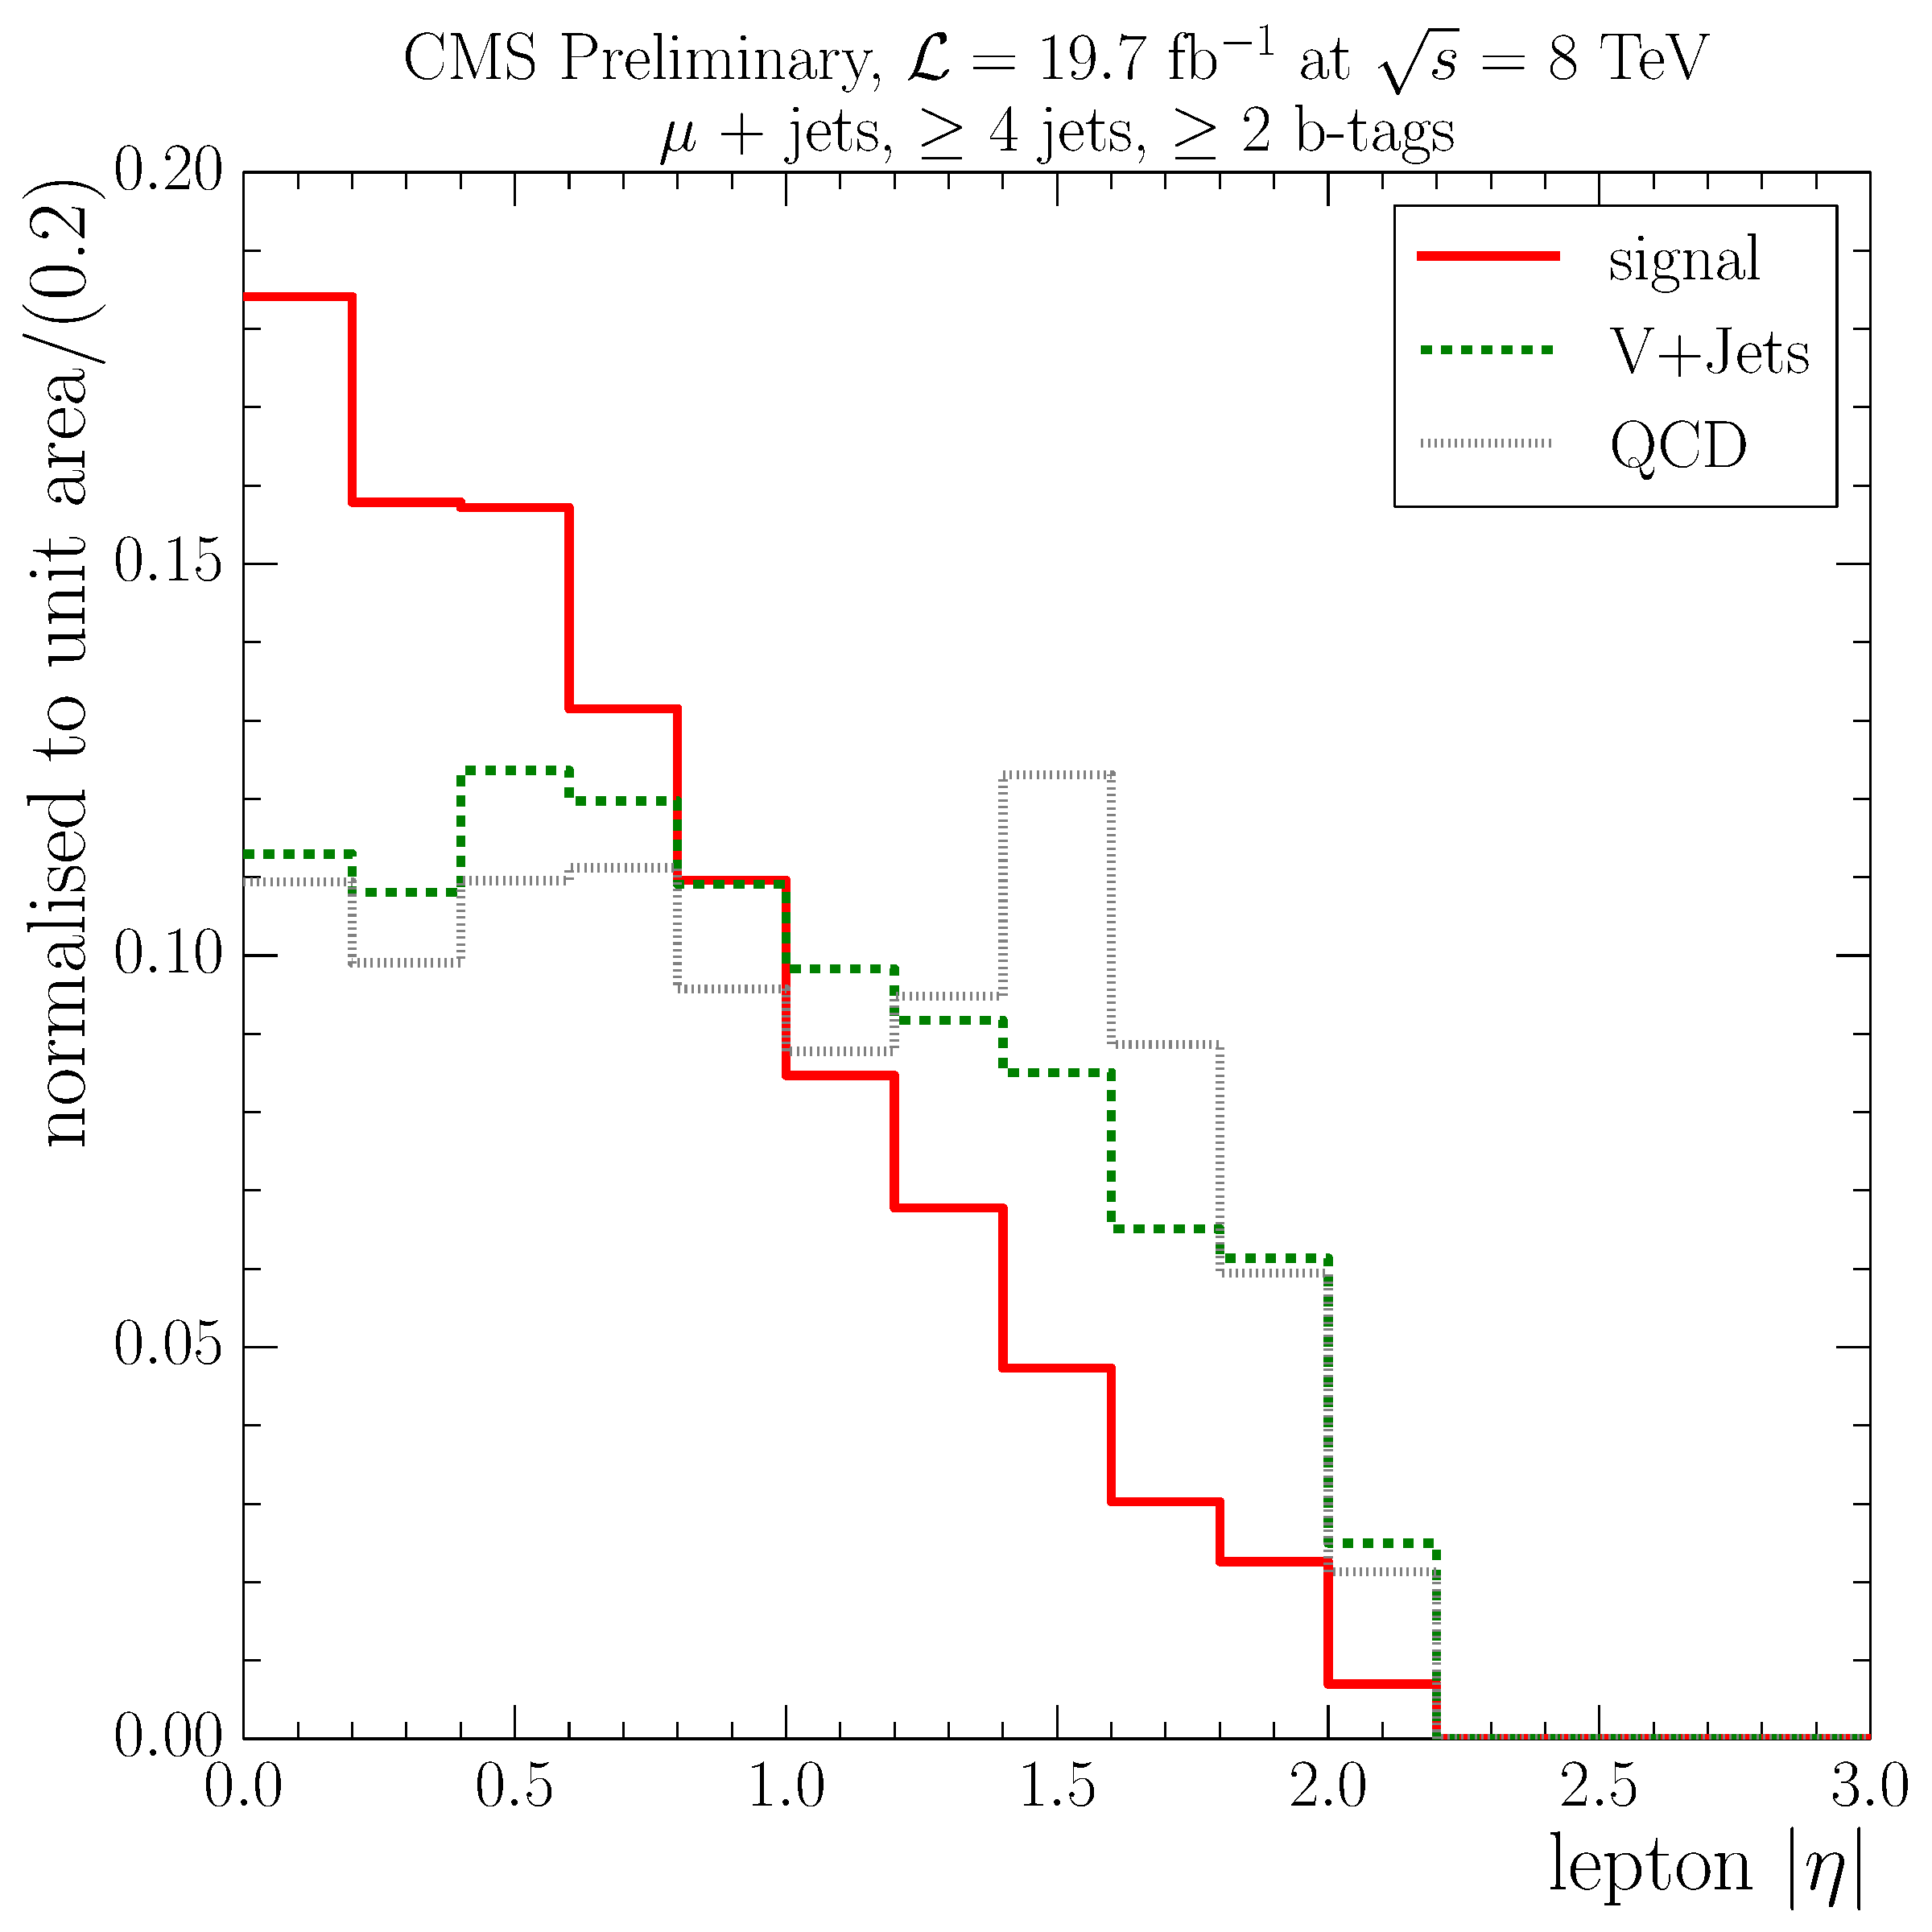
\includegraphics[width=0.42\textwidth]{measurement/MET/central/fit_templates/muon_templates_bin_150-inf}}
  	\hspace*{\fill}
    \caption[Muon $\abs \eta$ templates for the fit in different bins of \MET]{Muon $\abs \eta$ templates for the fit in
    different bins of \MET, from top left to bottom right: \SIrange{0}{25}{\GeV}, \SIrange{25}{45}{\GeV},
    \SIrange{45}{70}{\GeV}, \SIrange{70}{100}{\GeV}, \SIrange{100}{150}{\GeV} and $\geq \SI{150}{\GeV}$.}
    \label{fig:fit_templates_MET_muon}
\end{figure}

\sisetup{range-phrase = {~to~}}
\sisetup{range-units = repeat}

The template fit is performed independently in each primary variable bin by minimising the log-likelihood defined as:
% \begin{align}
% LL\left(\Niexp,N_i^\text{obs}\right) &=-2\,\log{\left(\prod\limits_{i}\frac{\left(\Niexp\right)^{\Niobs}\cdot
% e^{-\Niexp}}{\Niobs!}\right)} \\
%  & =-2\sum\limits_{i}\log{\left(\frac{\left(\Niexp\right)^{\Niobs}\cdot e^{-\Niexp}}{\Niobs!}\right)}
% \end{align}
\begin{equation}
\label{eq:xsection_loglikelihood}
LL(\lambda_i,d_i)=-2\,\log{\left(\prod\limits_{i}\frac{\lambda_i^{d_i}\cdot
e^{-\lambda_i}}{d_i!}\right)}=-2\sum\limits_{i}\log{\left(\frac{\lambda_i^{d_i}\cdot e^{-\lambda_i}}{d_i!}\right)},
\end{equation}
where $\lambda_i$ is the sum of expected events from all the templates $d_i$ is the number of data events in each bin
$i$, and summation is performed over all bins $i$ of the $\abs {\eta_l}$ distribution. The expected lepton
pseudorapidity (array of $\lambda_i$) is modelled by normalising the templates $\theta_{i\,j}$ by normalisation factors
$N_j$:

\begin{equation}
\label{eq:xsection_templates_normalisation}
\lambda_i=\sum\limits_{j}N_j\theta_{i\,j},\;\mathrm{where}\;\sum\limits_{i}\theta_{i\,j}=1~\mathrm{for~every~process}~j.
\end{equation}

The minimisation of the log-likelihood is achieved by varying the fit parameters, i.e.\ normalisation factors for each
template. Therefore, the template fit strives for equality of $\lambda_i$ and $d_i$ in all lepton pseudorapidity bins.
The initial normalisation values for the templates are taken from the expected number of events for \ttbar, single top,
\WpJets and \ZpJets as per Table~\ref{tab:xsection_mc_samples}. Although the QCD template shape is data-driven, the
initial normalisation for it is also taken from Monte Carlo simulation (Tables~\ref{tab:xsection_electron_qcd_samples}
and \ref{tab:xsection_muon_qcd_samples}).

The similarity of QCD and \VpJets templates, particularly for muon plus jets events
(Figure~\ref{fig:fit_templates_MET_muon}), can lead to unphysical bin-to-bin fluctuations of these backgrounds. To
mitigate such behaviour, the following conservative Gaussian constraints were added to the likelihood function of the
fit:

\begin{align}
\label{eq:xsection_fit_constraints}
(N_{\VpJets}^\mathrm{fit}-N_{\VpJets}^\mathrm{MC})^2/(0.5 \times N_{\VpJets}^\mathrm{MC})^2 \\
(N_\mathrm{QCD}^\mathrm{fit}-N_\mathrm{QCD}^\mathrm{MC})^2/(2\times N_\mathrm{QCD}^\mathrm{MC})^2
\end{align}

The first term represents the constraint of the number of \VpJets events to within \SI{50}{\pc} of that predicted by
theory, whereas the second term is a \SI{200}{\pc} constraint for QCD events.

Figure~\ref{fig:fitted_MET} shows the control plots of data/MC comparison for the \MET variable in both electron and
muon channels. Here the normalisation for signal and backgrounds is taken from the fitted results. Similar plots for \HT
and \ST are shown in Figure~\ref{fig:fitted_HT_ST}, whereas Figure~\ref{fig:fitted_WPT_MT} shows control plots for \WPT
and \MT. Overall, the data and simulation agree within the fit uncertainty. The observed discrepancies can be attributed
to the known issue of the event generators incorrectly modelling the \pt spectrum of the top quarks
\autocite{ttbar_differential_xsection_7TeV, ttbar_differential_xsection_8TeV}. This effect is accounted for as a source
of systematic uncertainty, as explained in Section~\ref{s_xsection:systematics}.
%https://twiki.cern.ch/twiki/bin/viewauth/CMS/TopPtReweighting

\begin{figure}[!htbp]
	\centering
  	\subfloat[]{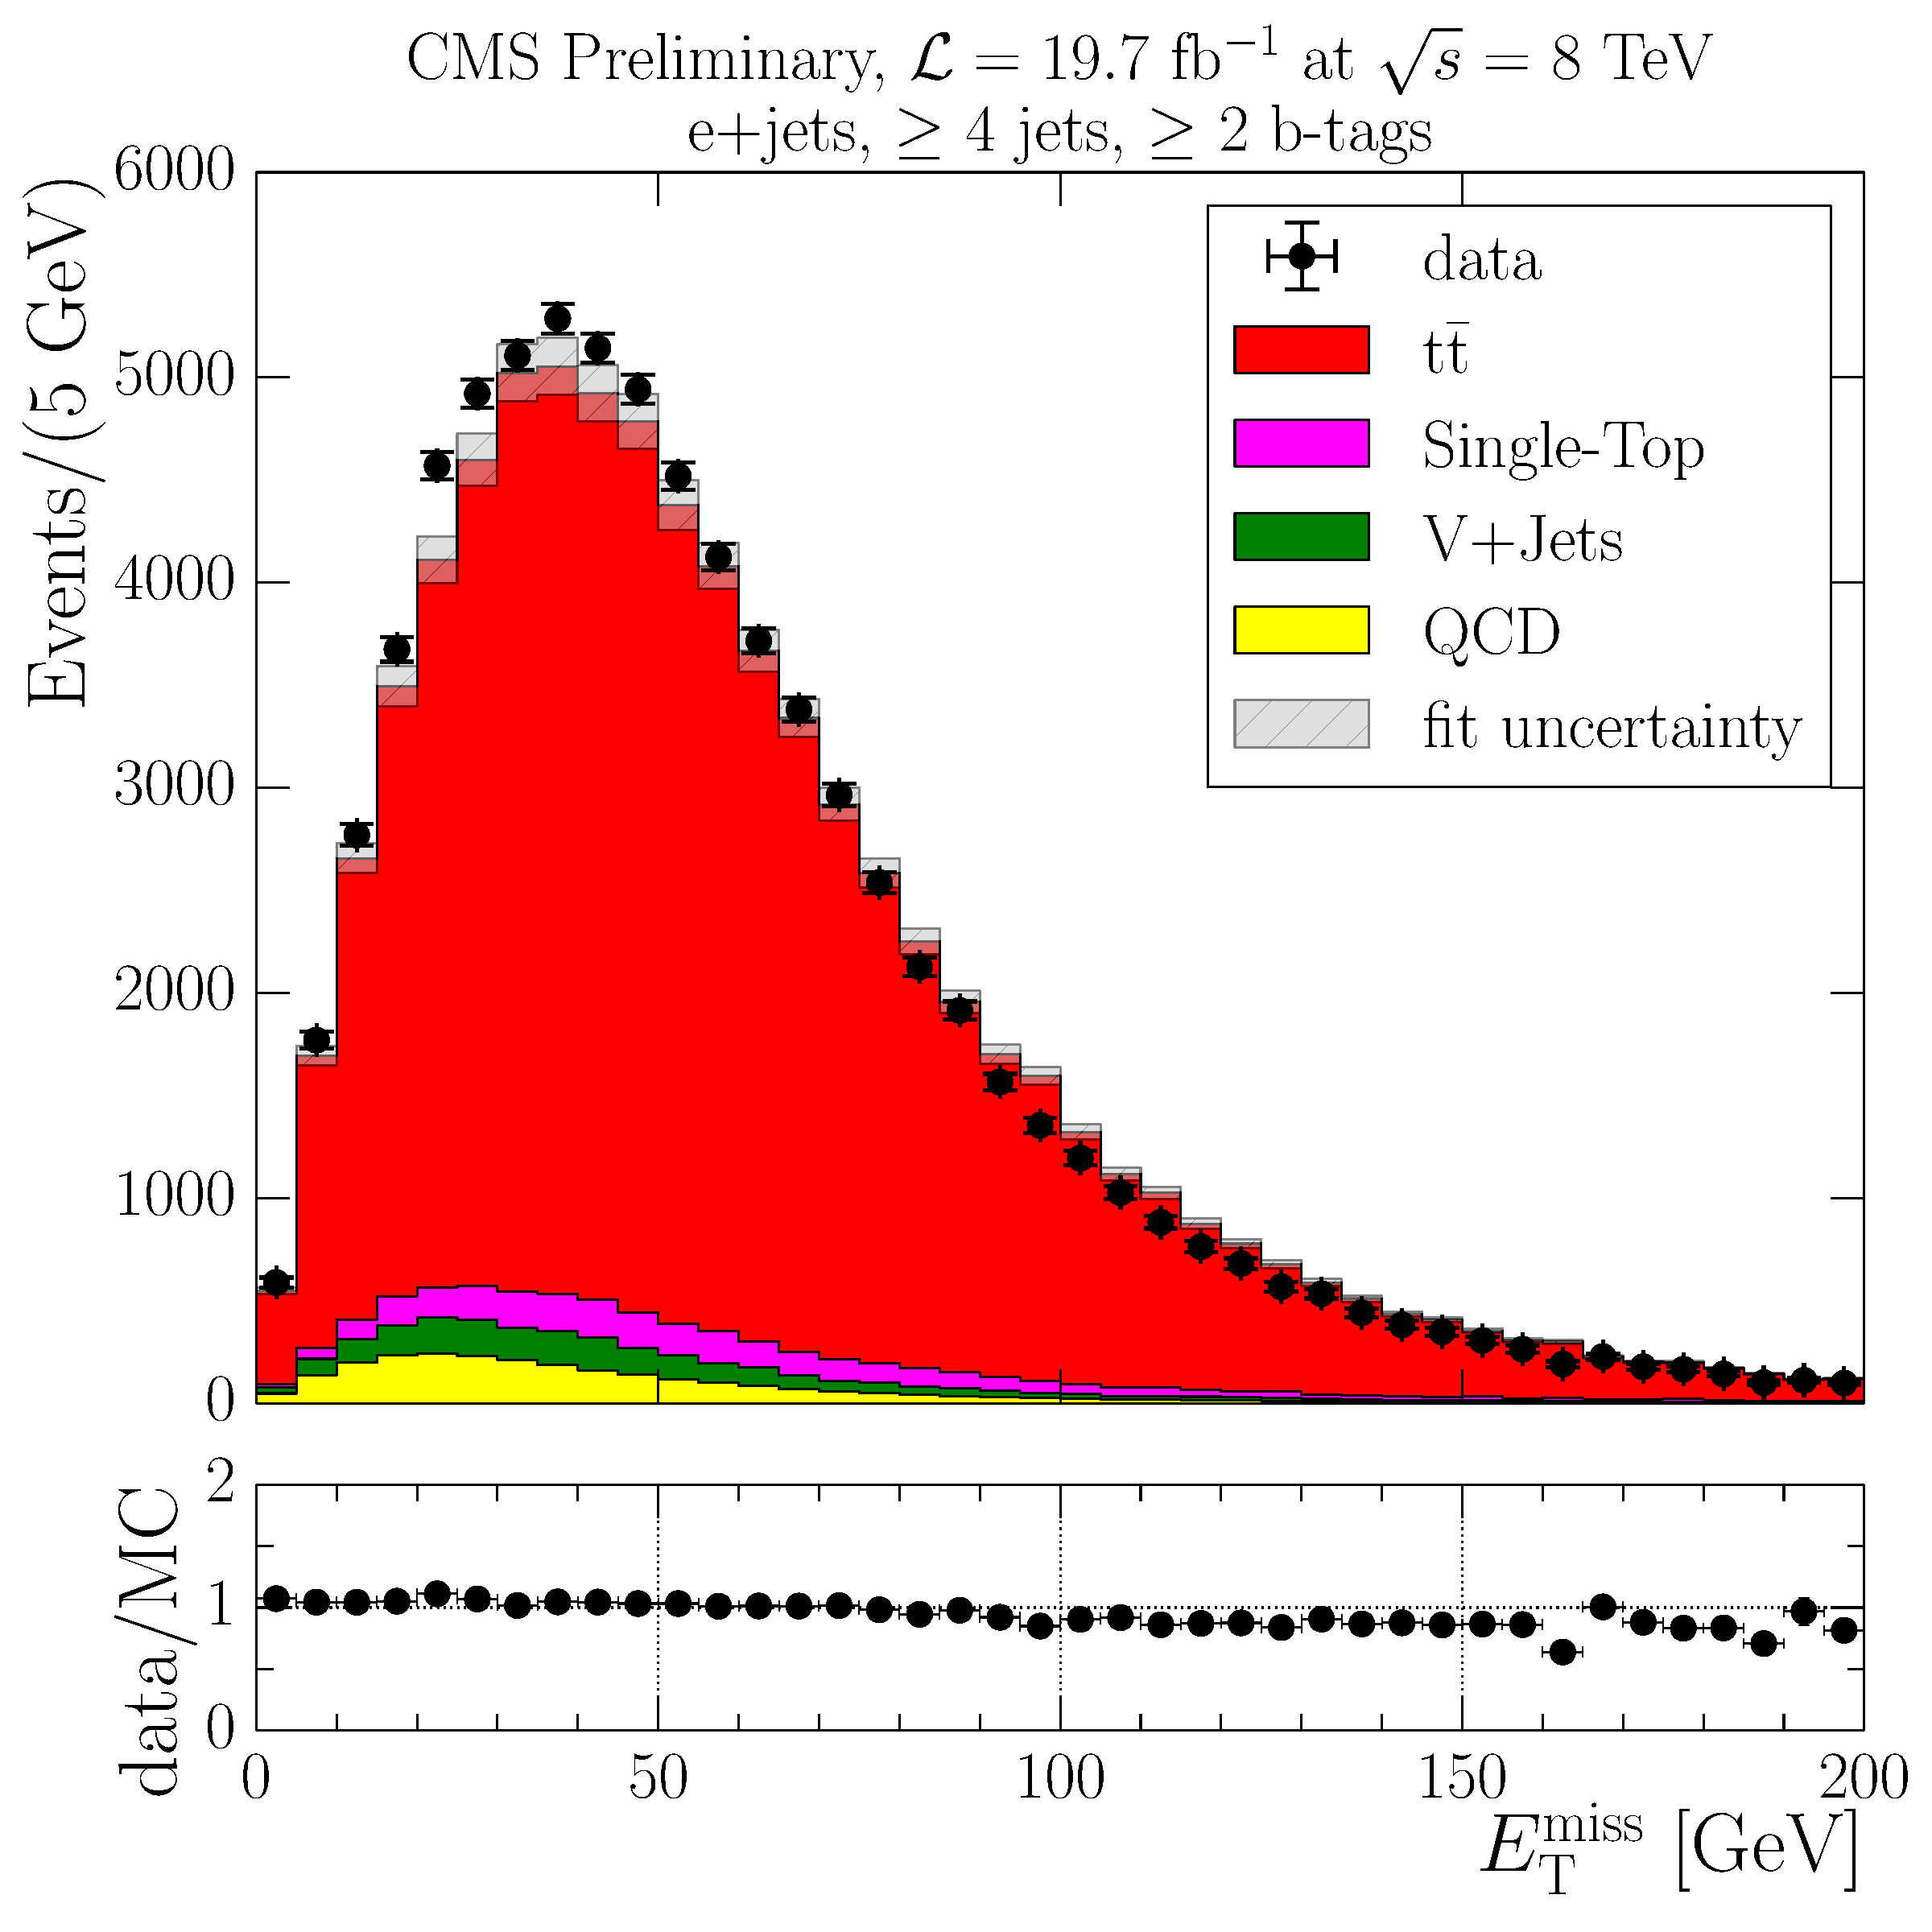
\includegraphics[width=0.5\textwidth]{fitted_primary_variables/EPlusJets_patType1CorrectedPFMet_2orMoreBtags_with_ratio}}\hfill
  	\subfloat[]{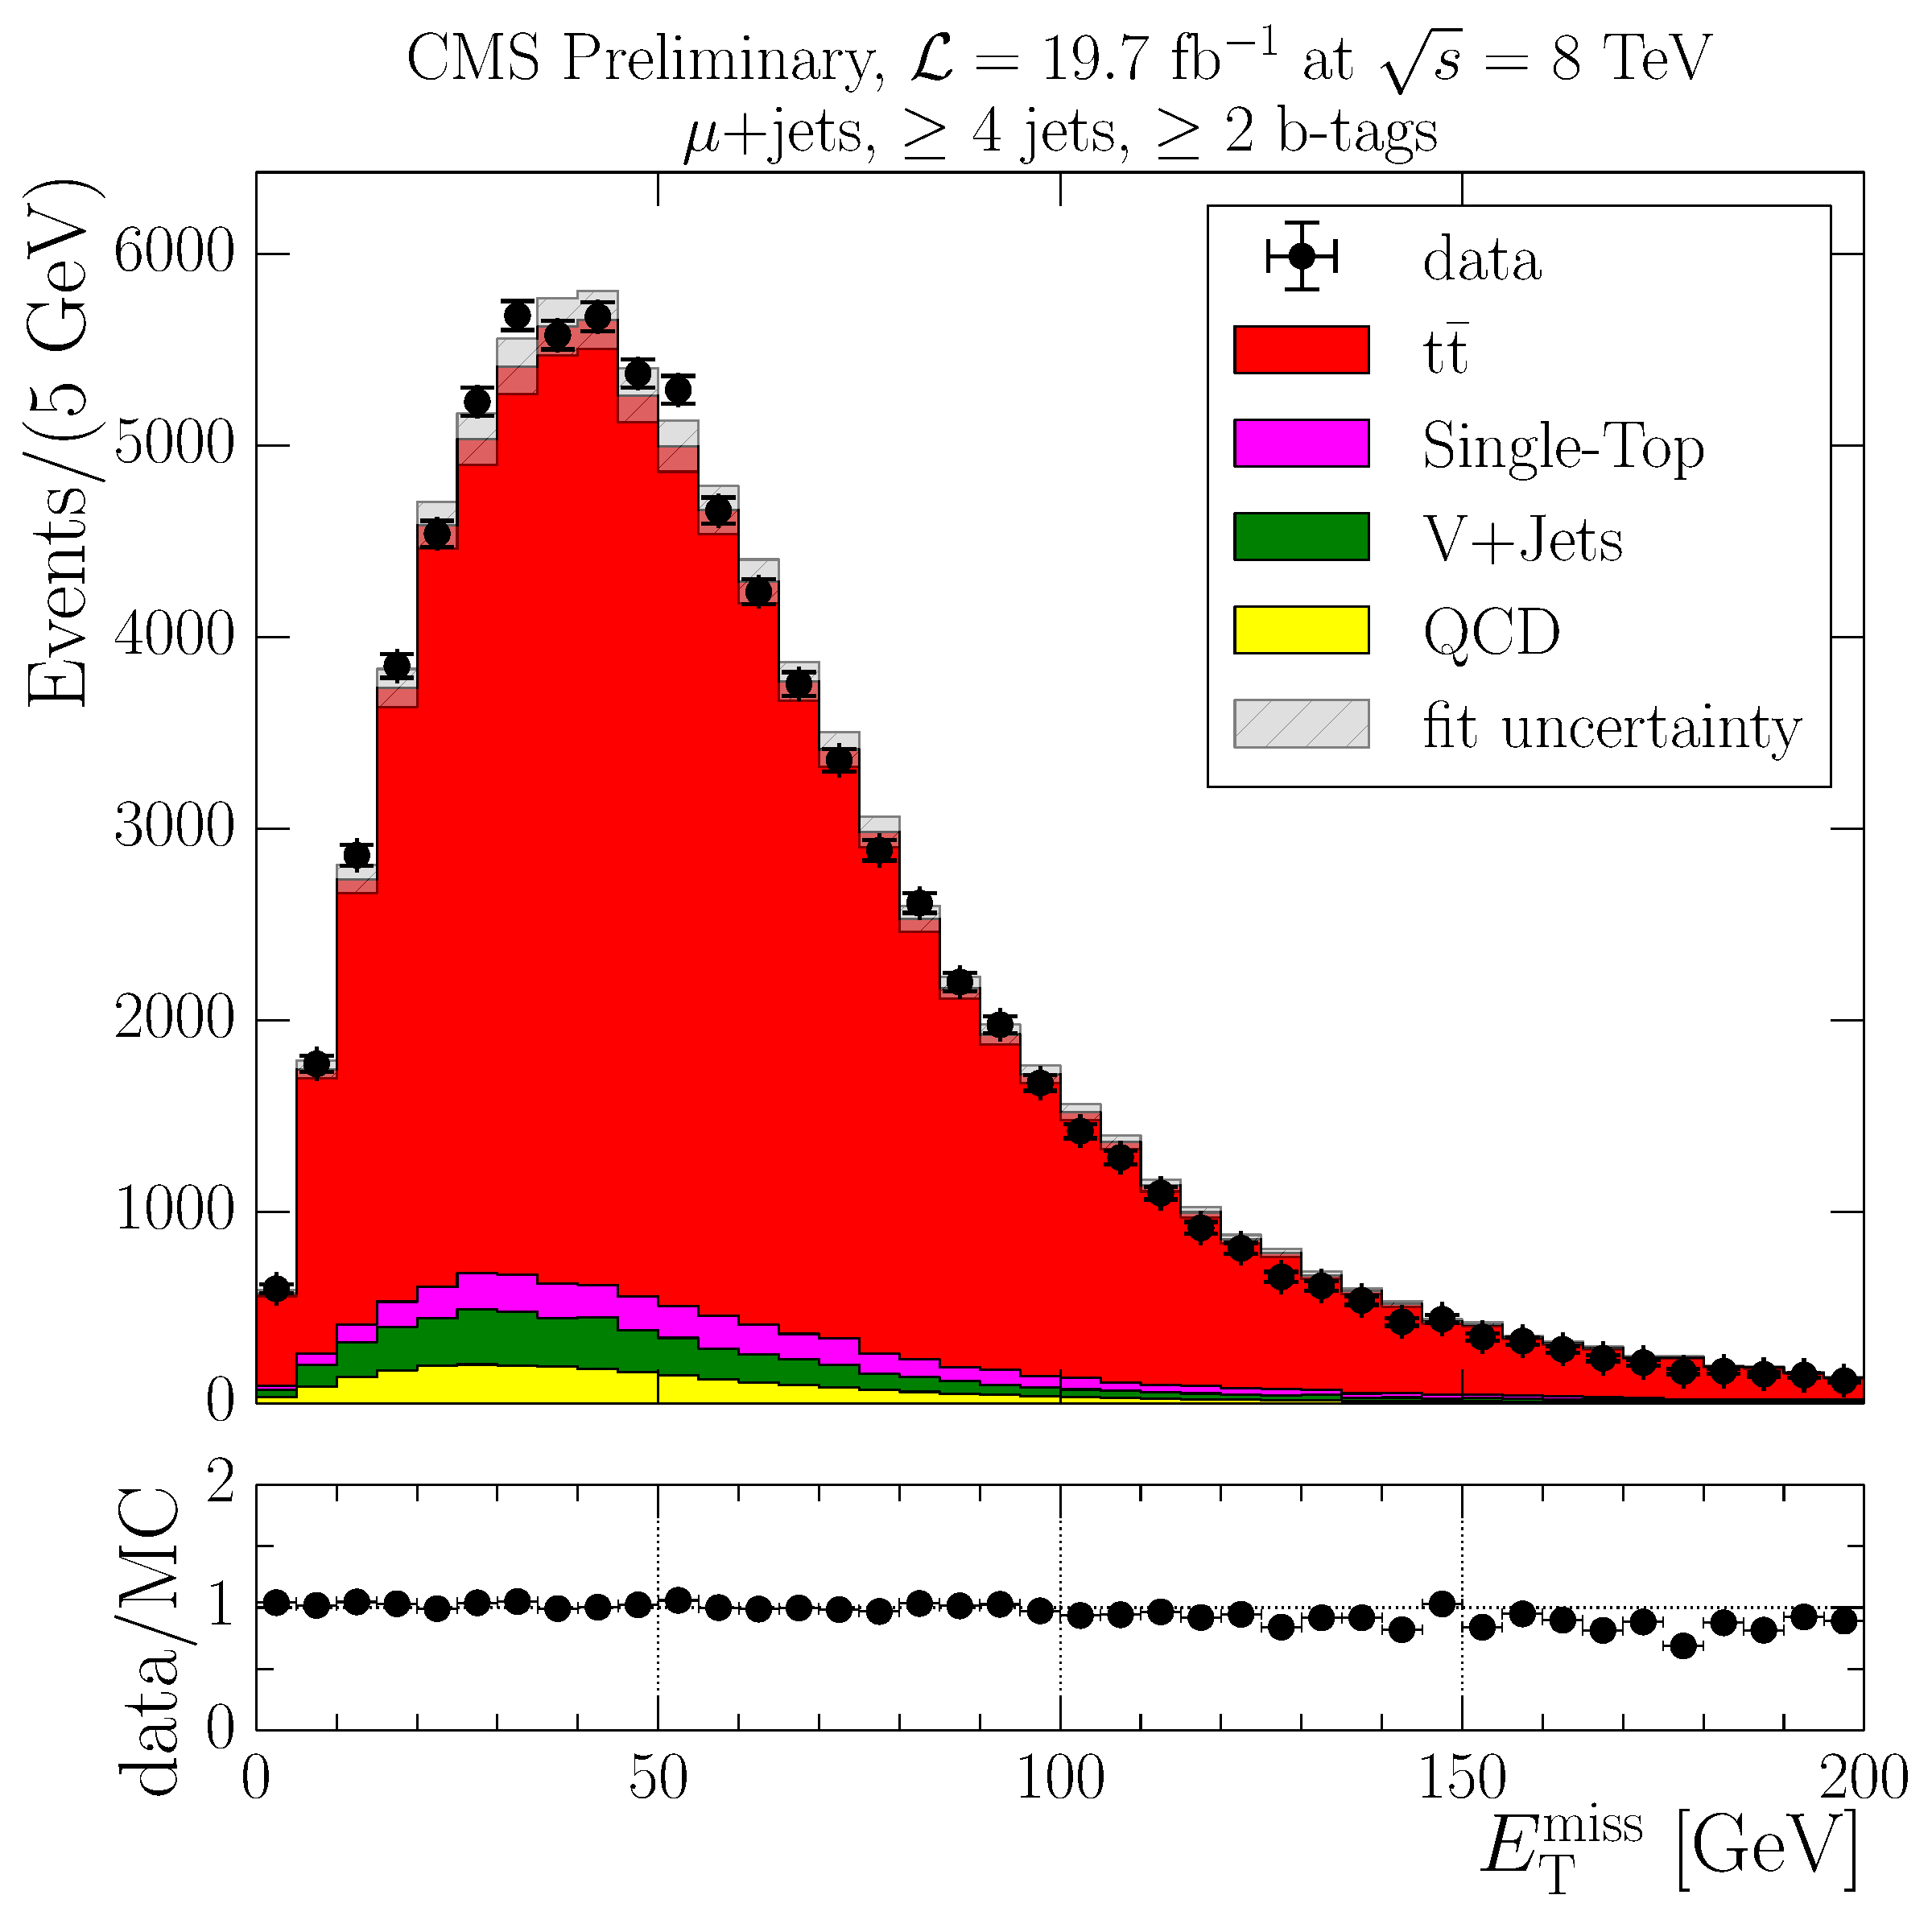
\includegraphics[width=0.5\textwidth]{fitted_primary_variables/MuPlusJets_patType1CorrectedPFMet_2orMoreBtags_with_ratio}}
    \caption[Data/MC comparison plots of \MET using the normalisation from the fitted results]{Data/MC comparison plots
    of \MET for electron plus jets (a) and muon plus jets (b) events after the final event selection using the
    normalisation from the fitted results.}
    \label{fig:fitted_MET}
\end{figure}

\begin{figure}[!htbp]
	\centering
  	\subfloat[]{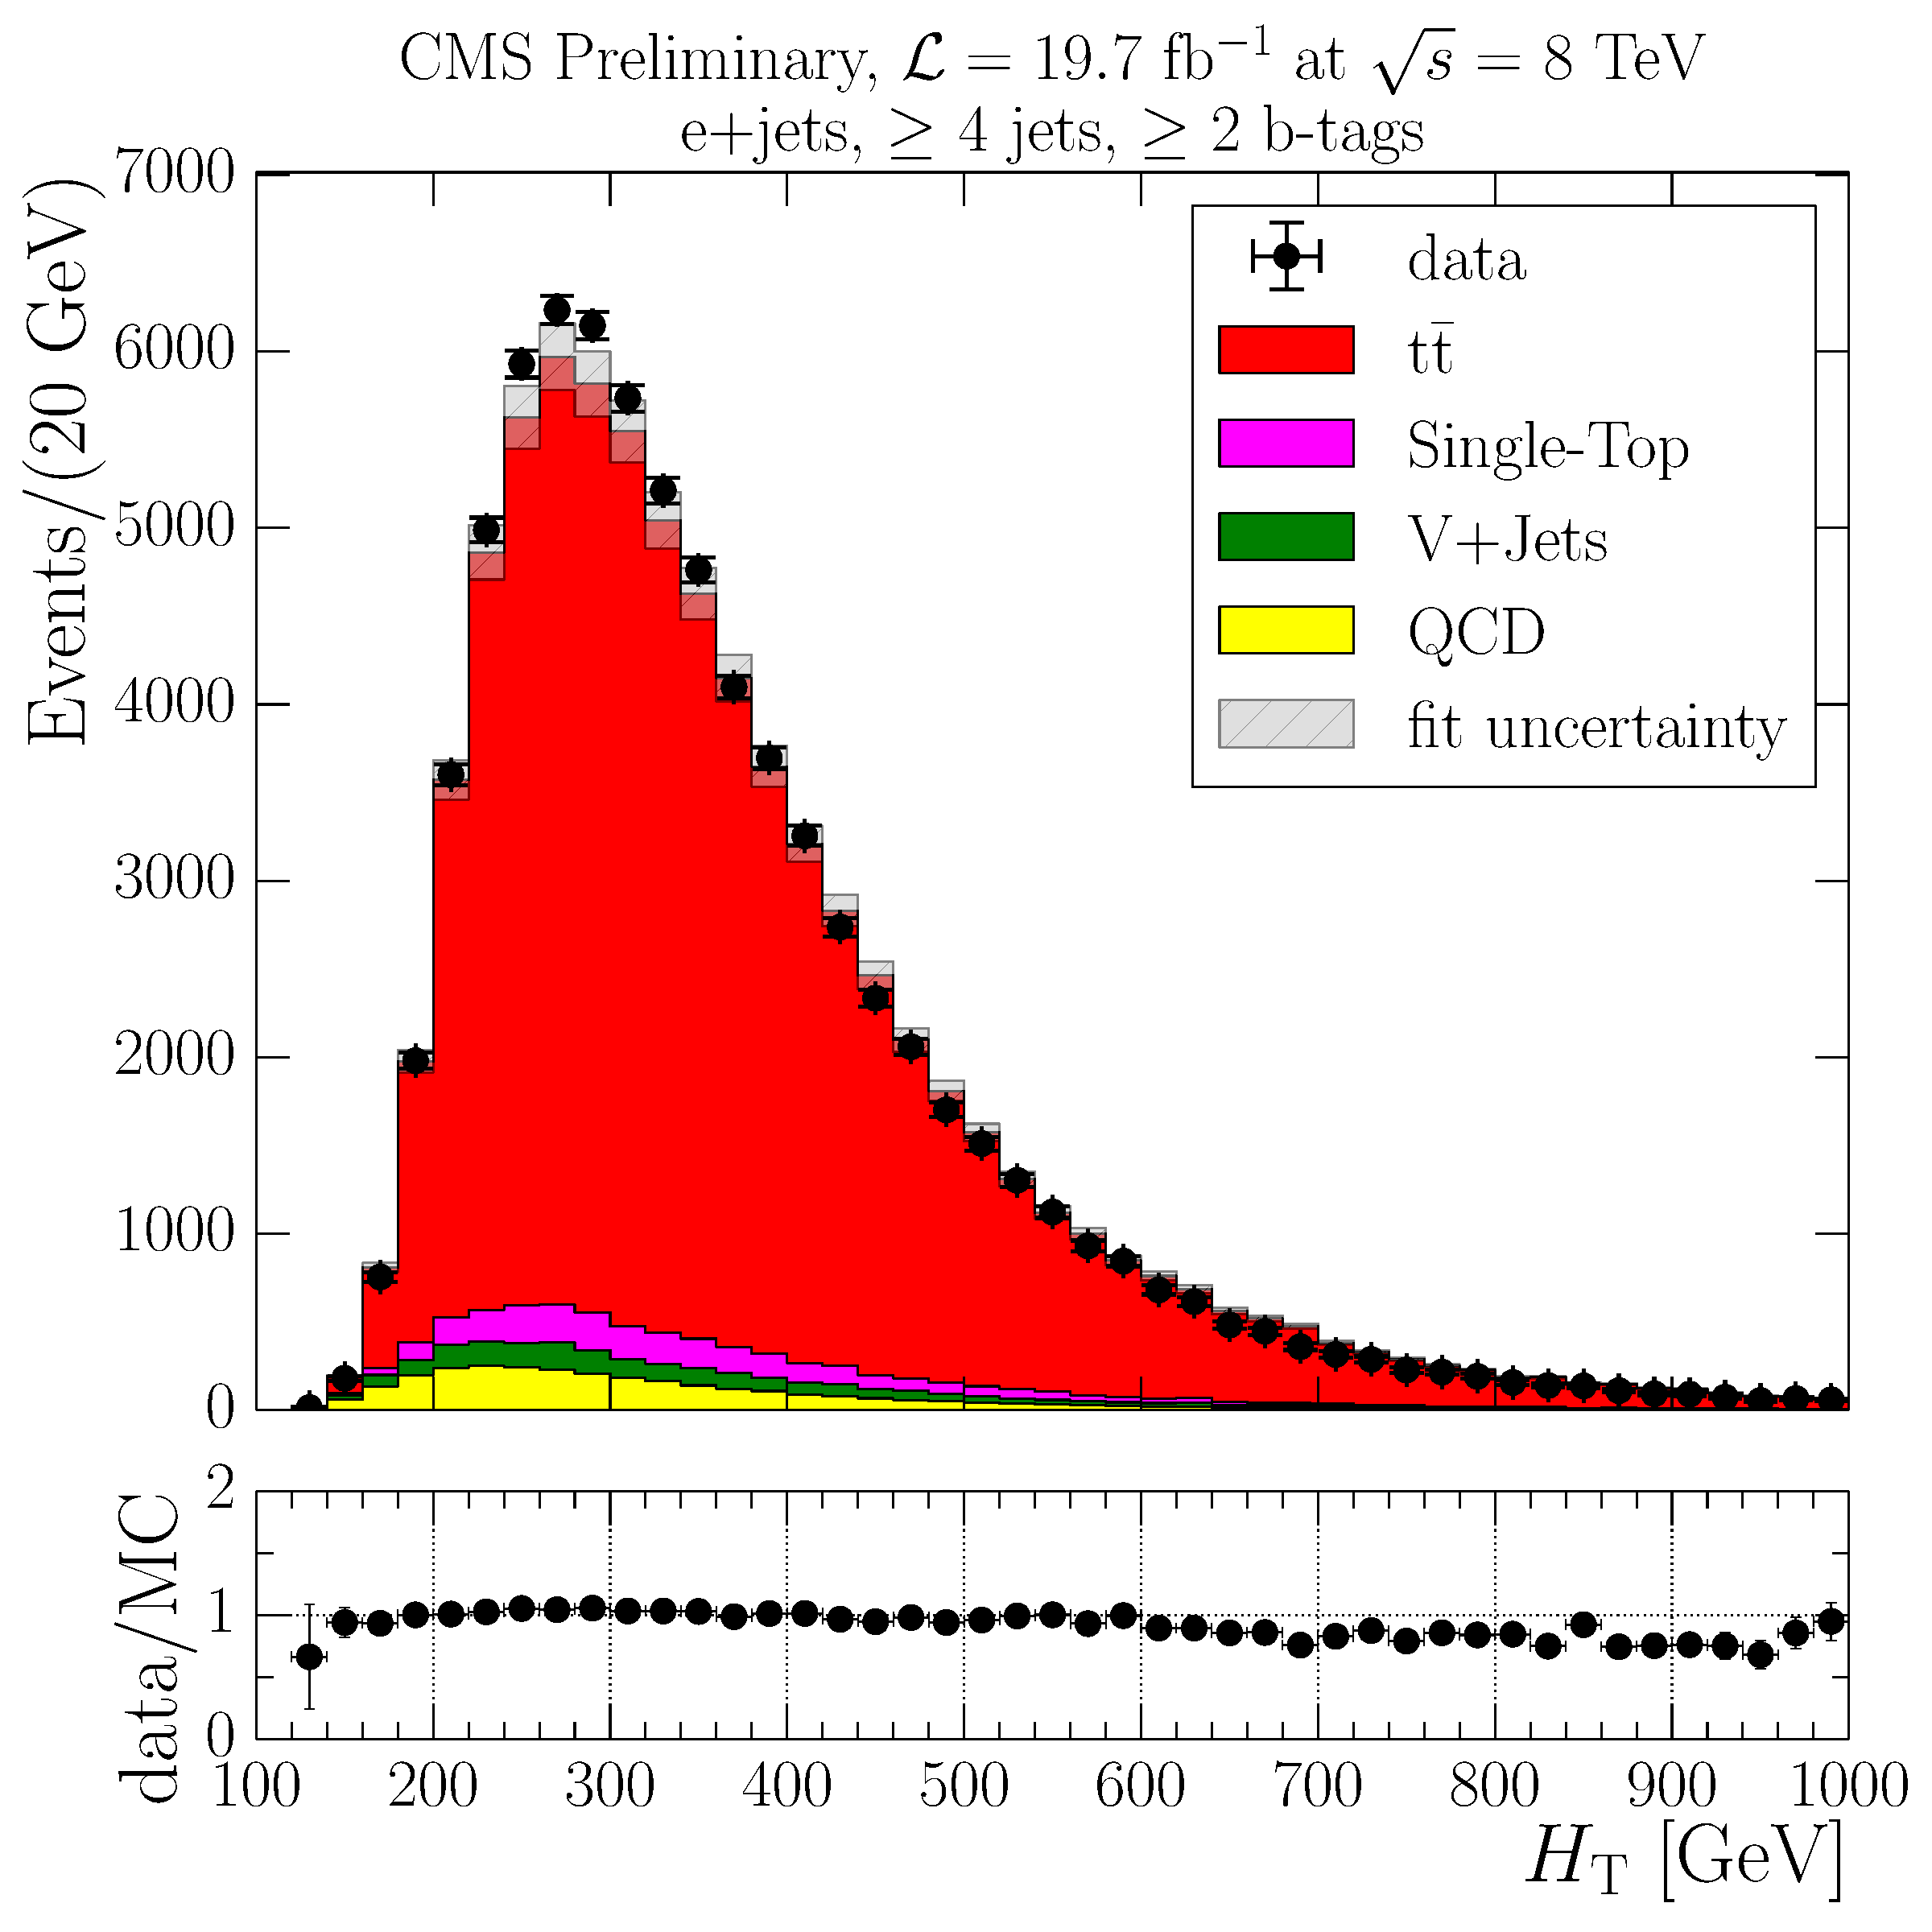
\includegraphics[width=0.5\textwidth]{fitted_primary_variables/EPlusJets_HT_2orMoreBtags_with_ratio}}\hfill
  	\subfloat[]{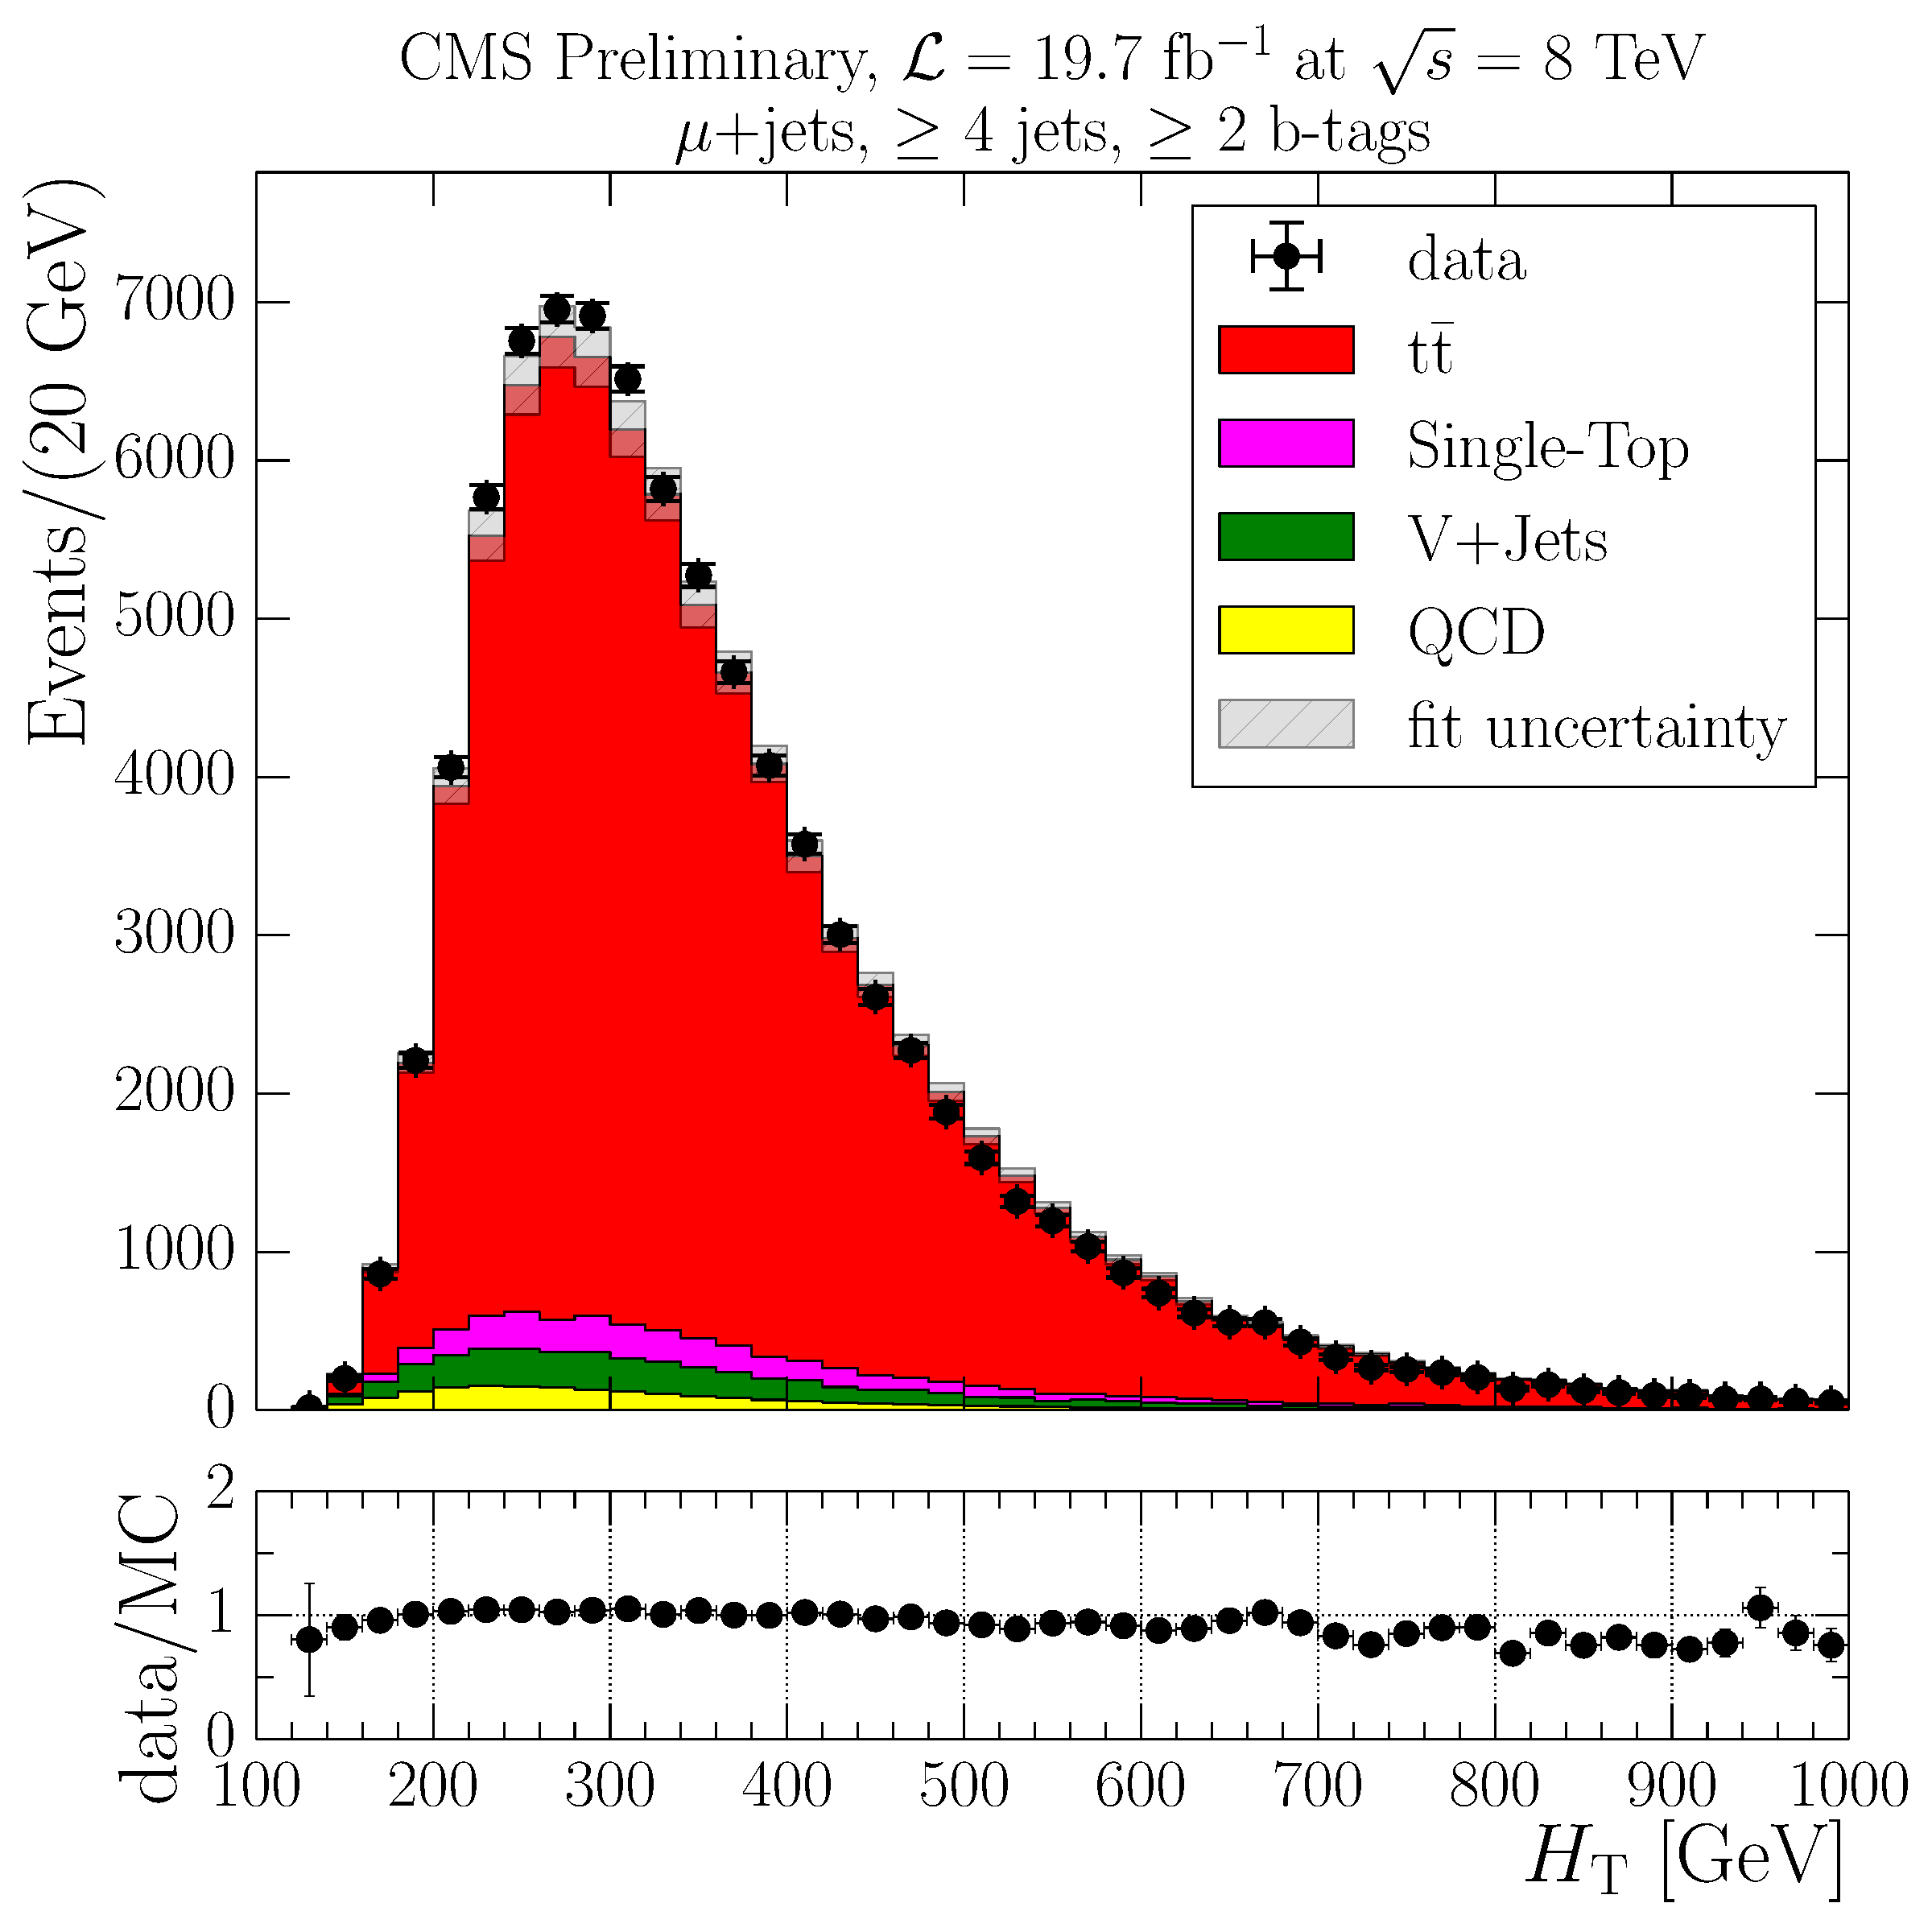
\includegraphics[width=0.5\textwidth]{fitted_primary_variables/MuPlusJets_HT_2orMoreBtags_with_ratio}} \\
  	\subfloat[]{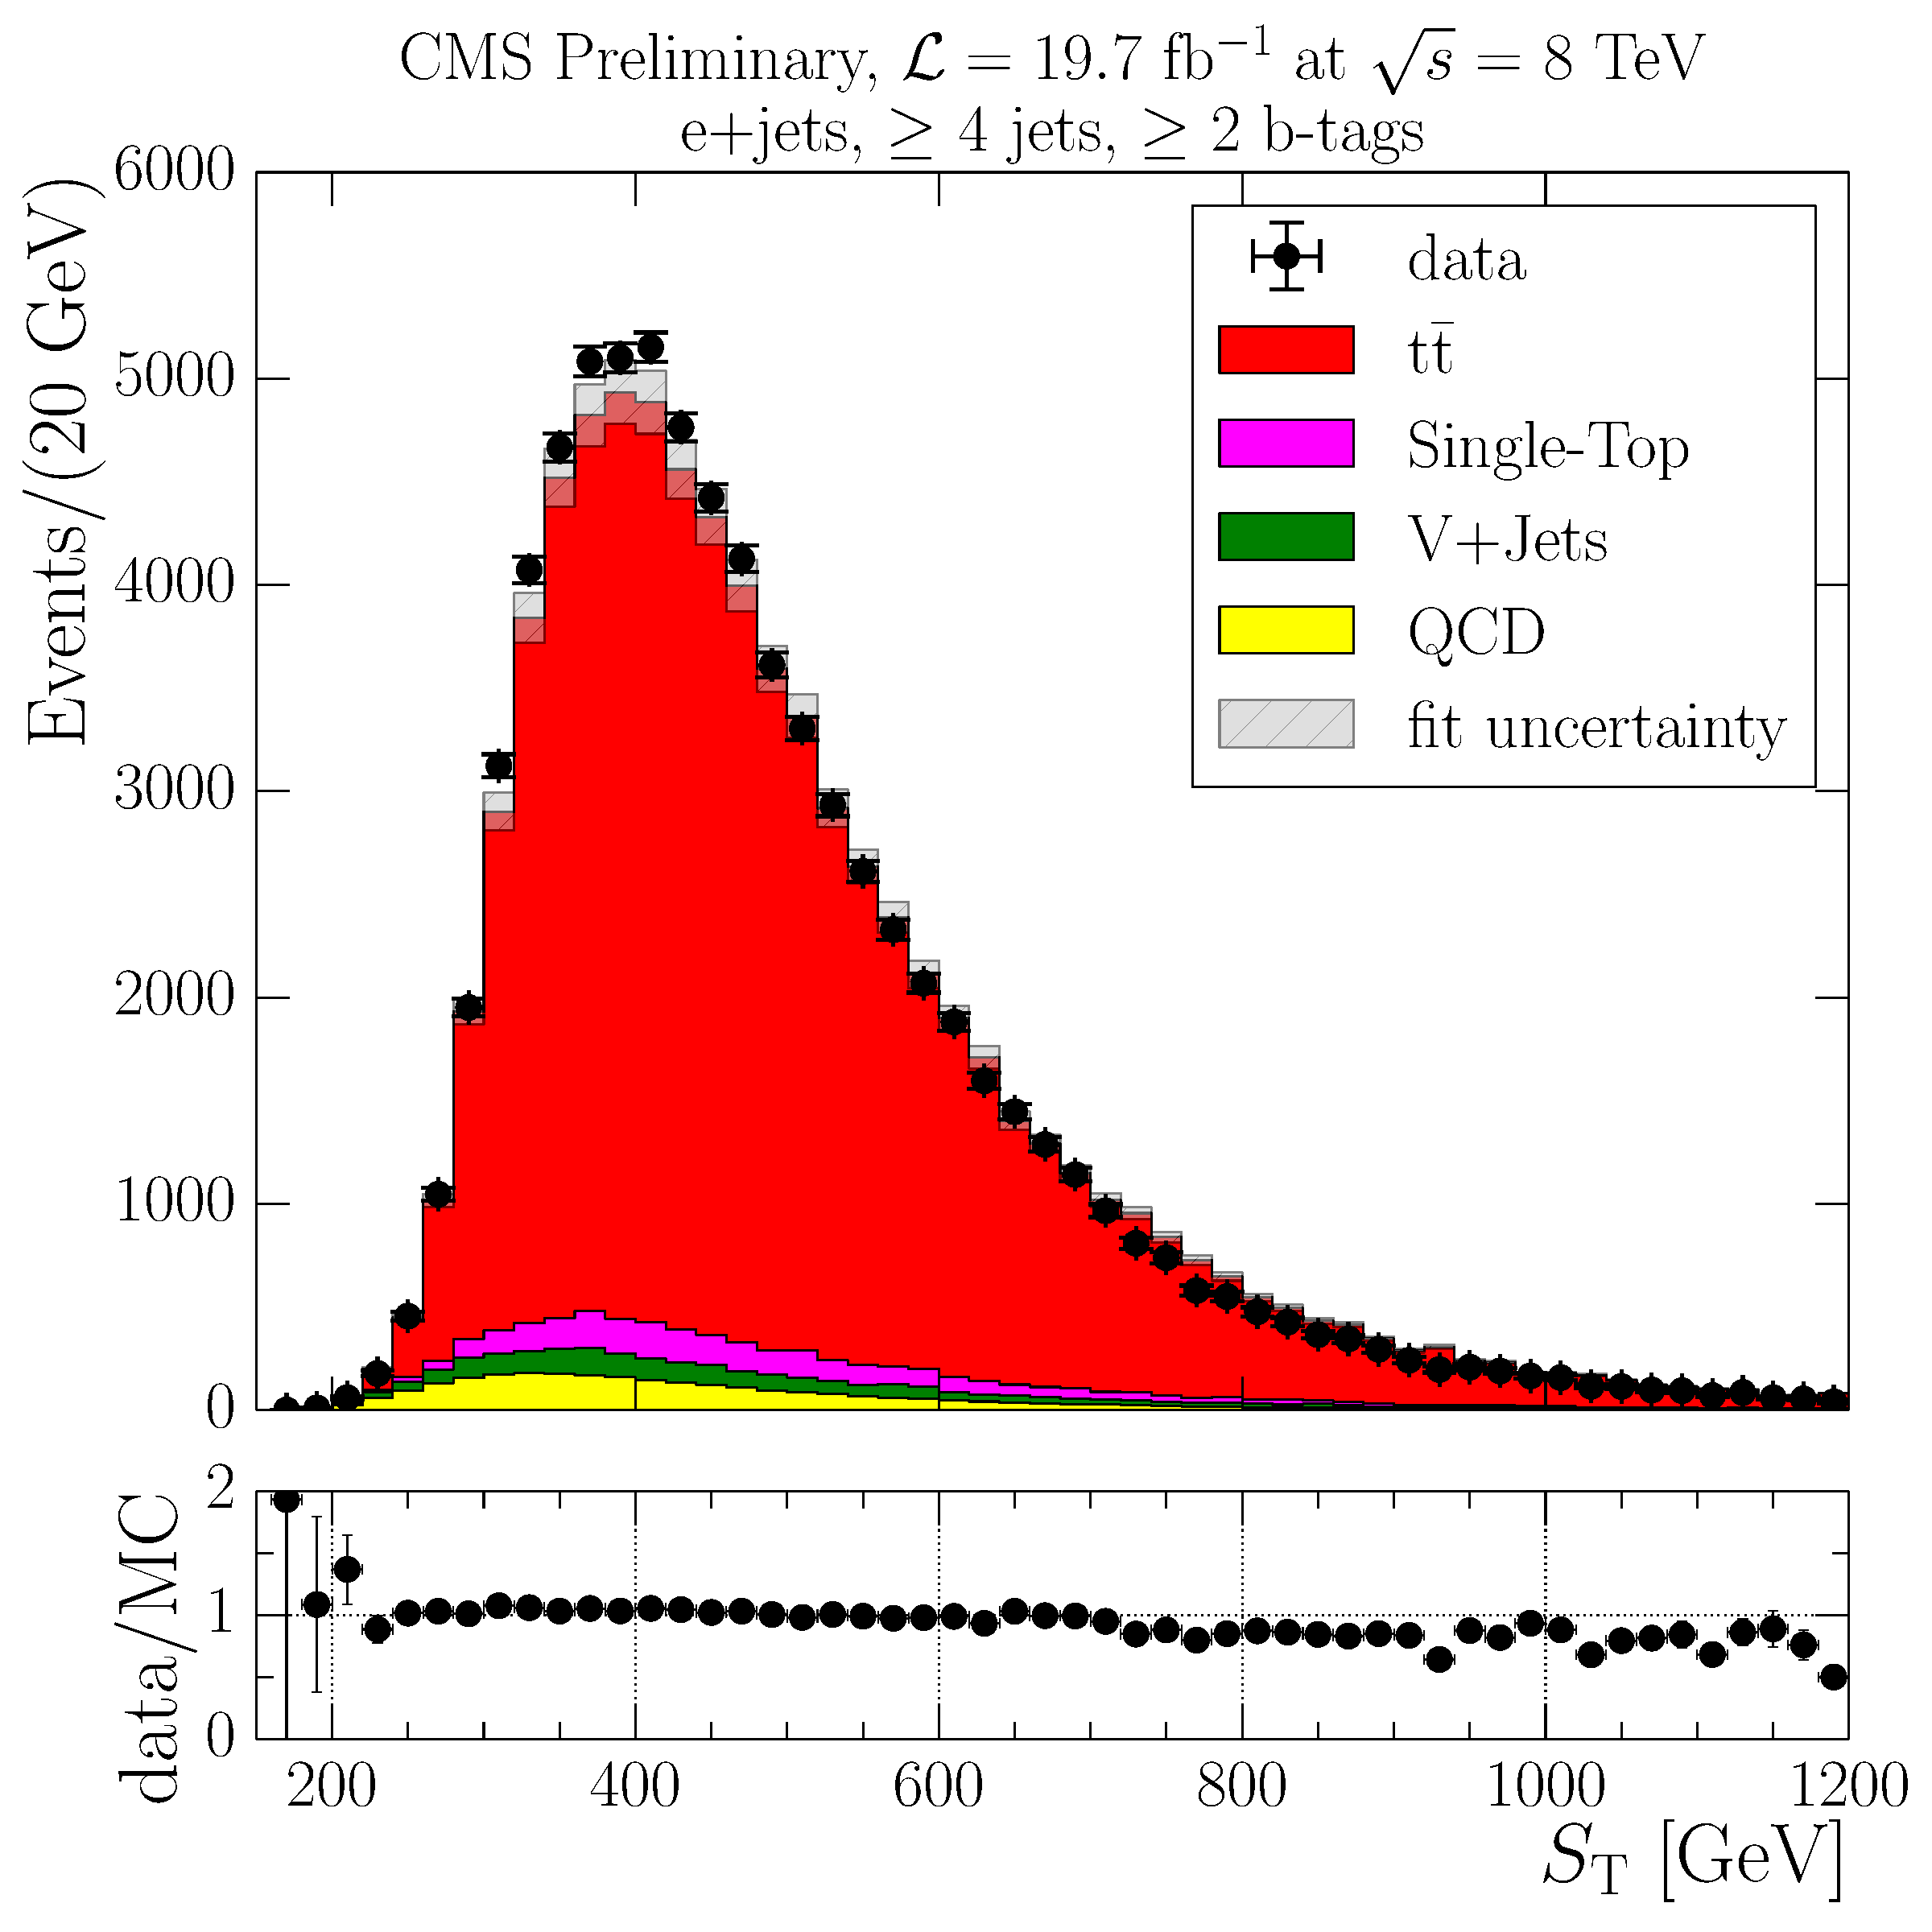
\includegraphics[width=0.5\textwidth]{fitted_primary_variables/EPlusJets_patType1CorrectedPFMet_ST_2orMoreBtags_with_ratio}}\hfill
  	\subfloat[]{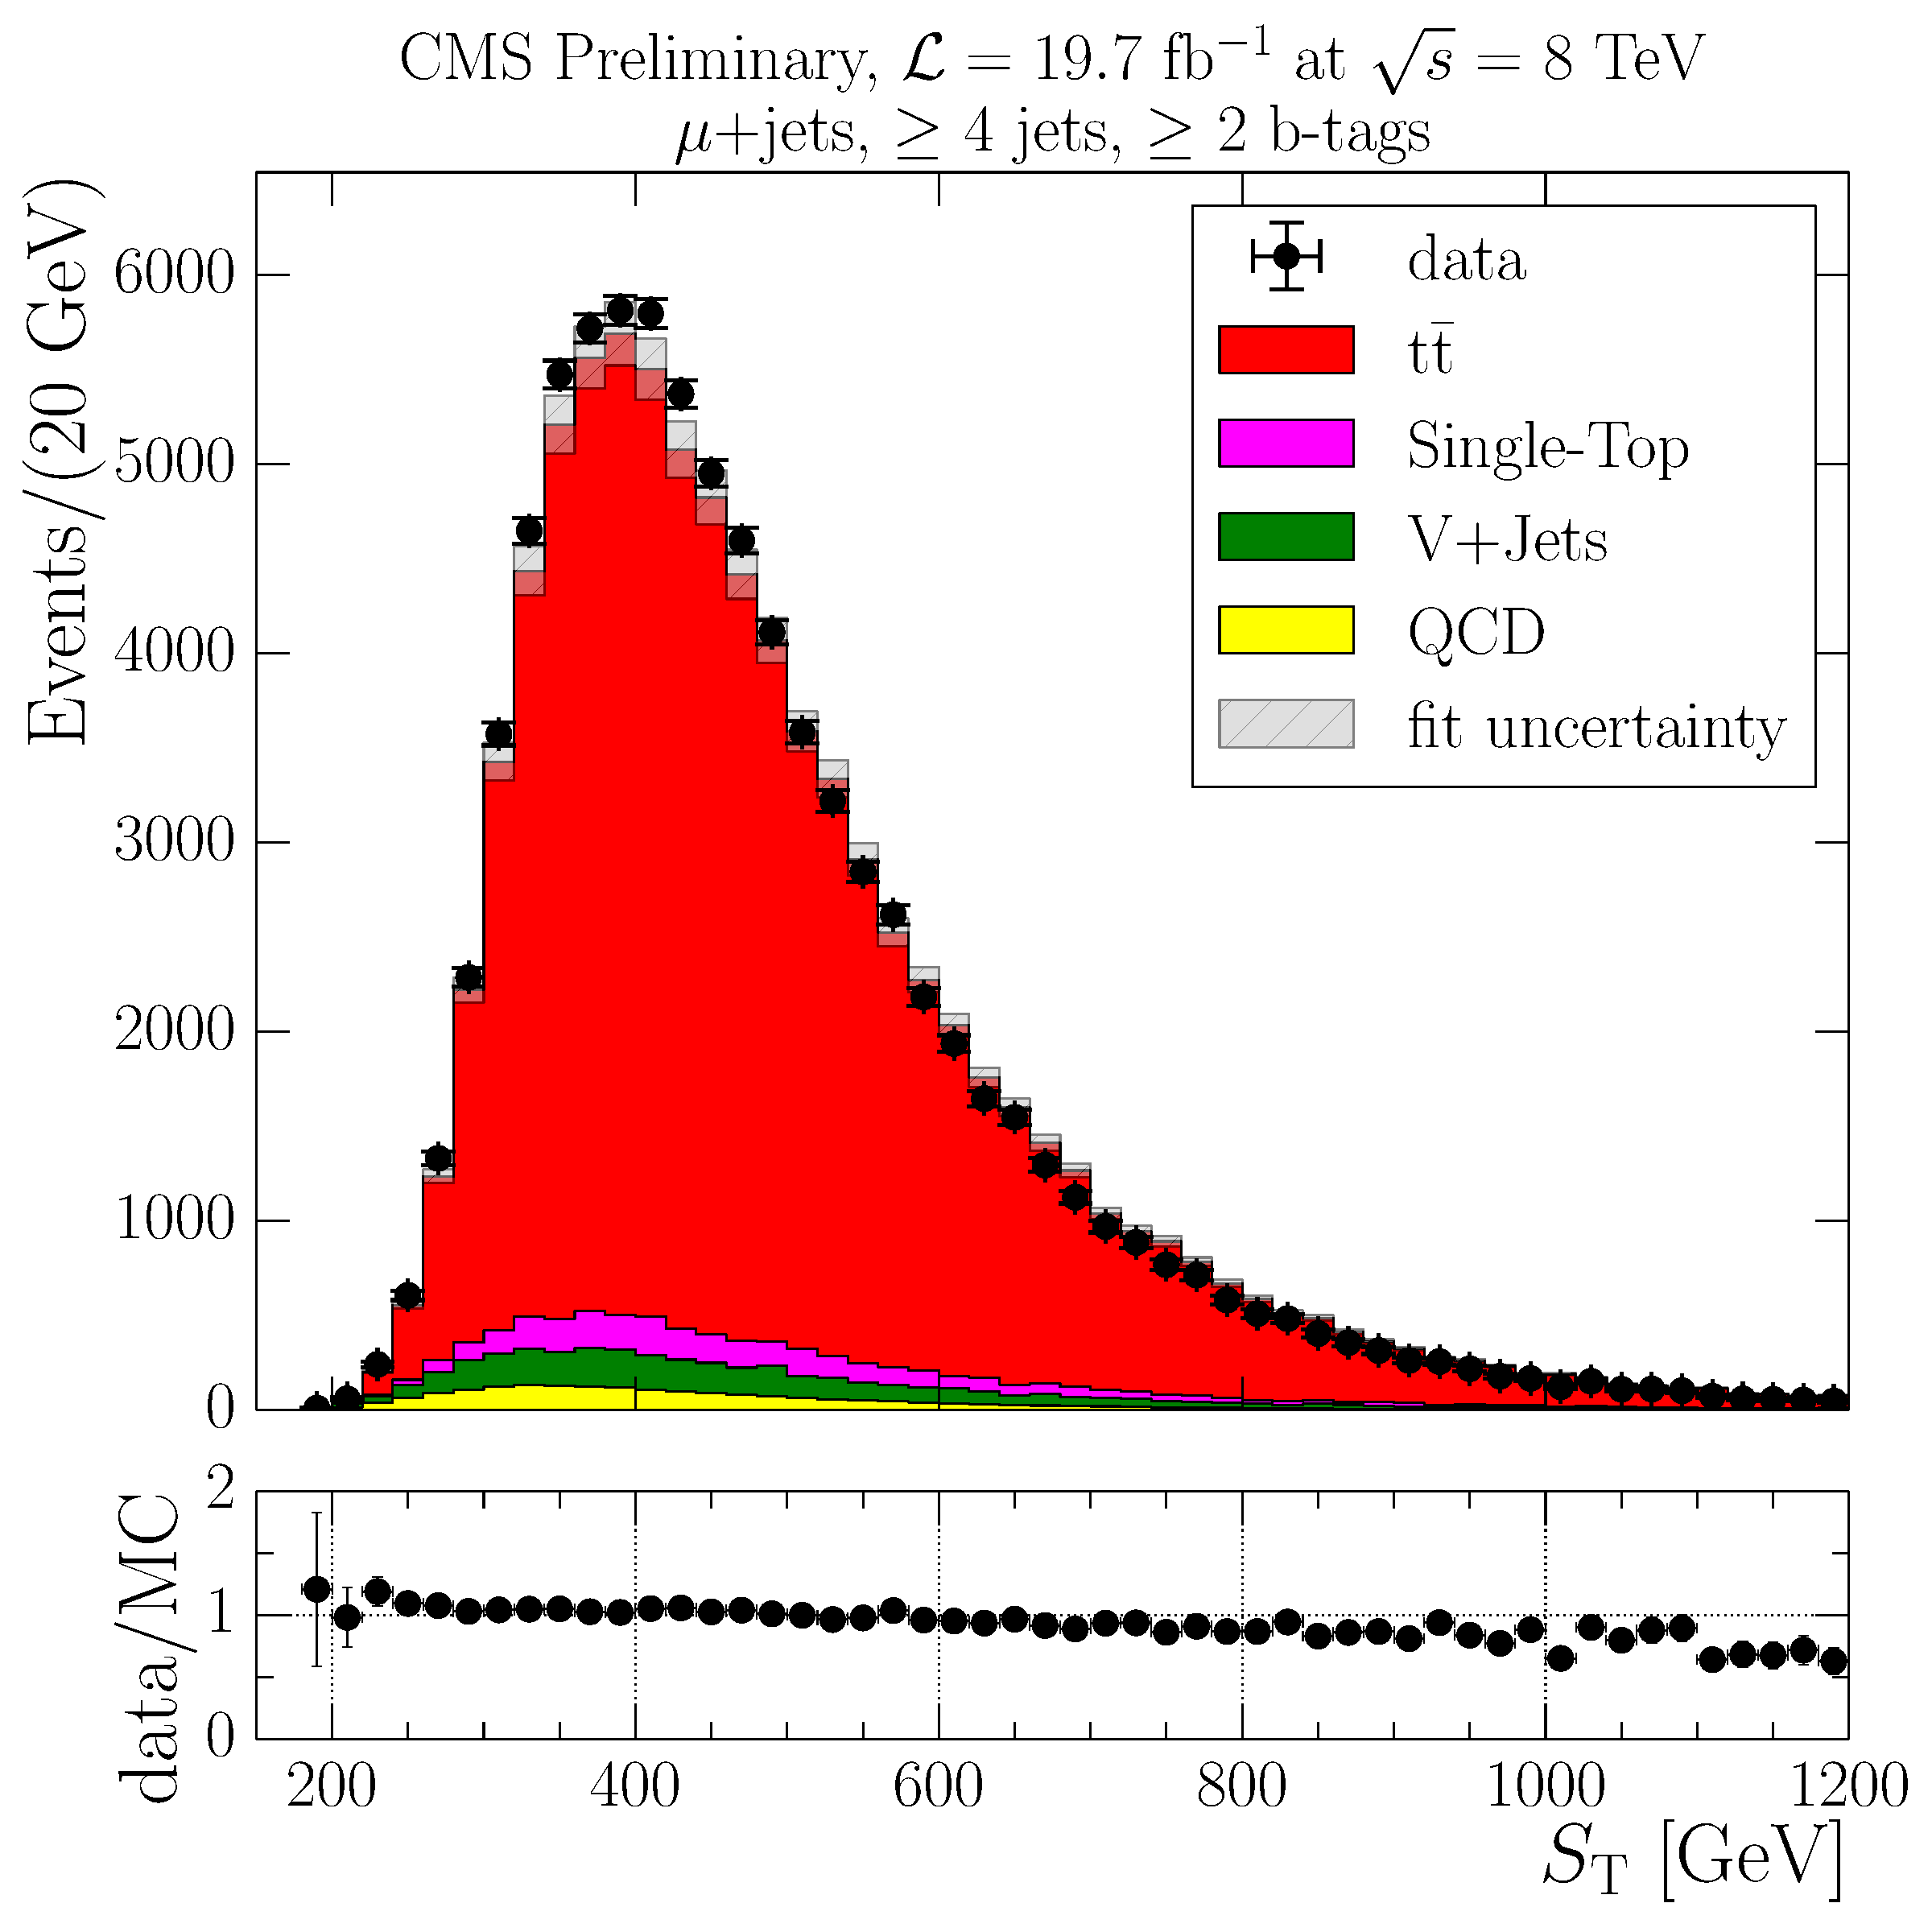
\includegraphics[width=0.5\textwidth]{fitted_primary_variables/MuPlusJets_patType1CorrectedPFMet_ST_2orMoreBtags_with_ratio}}
    \caption[Data/MC comparison plots of \HT and \ST using the normalisation from the fitted results]{Data/MC comparison
    plots of \HT (a, b) and \ST (c, d) after the final event selection using the normalisation from the fitted results.
    Left-hand plots: electron plus jets selection, right-hand plots: muon plus jets selection.}
    \label{fig:fitted_HT_ST}
\end{figure}

\begin{figure}[!htbp]
	\centering
  	\subfloat[]{\includegraphics[width=0.5\textwidth]{fitted_primary_variables/EPlusJets_patType1CorrectedPFMet_WPT_2orMoreBtags_with_ratio}}\hfill
  	\subfloat[]{\includegraphics[width=0.5\textwidth]{fitted_primary_variables/MuPlusJets_patType1CorrectedPFMet_WPT_2orMoreBtags_with_ratio}} \\
  	\subfloat[]{\includegraphics[width=0.5\textwidth]{fitted_primary_variables/EPlusJets_patType1CorrectedPFMet_MT_2orMoreBtags_with_ratio}}\hfill
  	\subfloat[]{\includegraphics[width=0.5\textwidth]{fitted_primary_variables/MuPlusJets_patType1CorrectedPFMet_MT_2orMoreBtags_with_ratio}}
    \caption[Data/MC comparison plots of \WPT and \MT using the normalisation from the fitted results]{Data/MC
    comparison plots of \WPT (a, b) and \MT (c, d) after the final event selection using the normalisation from the
    fitted results. Left-hand plots: electron plus jets selection, right-hand plots: muon plus jets selection.}
    \label{fig:fitted_WPT_MT}
\end{figure}

The output of the fit yields the number of top-like events in each bin, which includes both \ttbar and single top
processes since the lepton pseudorapidity distribution is very similar between them. The number of \ttbar events is
extracted from the signal fit result by using the expected ratio of \ttbar and single top events before the fitting
process:
\begin{equation}
\label{eq:xsection_decomposition}
\Nttbar^{\text{fit}} = N_{\text{signal}}^{\text{fit}} \times \frac{\Nttbar^{\text{exp}}}{N_{\text{signal}}^{\text{exp}}},
\end{equation}
where $N_{\ttbar}^{\text{fit}}$ ($N_{\text{signal}}^{\text{fit}}$) is the number of \ttbar (\ttbar + single top) events
as found by the fit, and $N_{\ttbar}^{\text{exp}}$ ($N_{\text{signal}}^{\text{exp}}$) is the number of \ttbar (\ttbar +
single top) events as predicted by theory.


\subsection{Unfolding}
\label{ss_xsection:unfolding}
Measurements of physical observables are inevitably distorted by various detector effects, including limited detector
resolution, experimental acceptance and selection inefficiency. Therefore, it is often very challenging to compare the
results with theory predictions, as well as other experiments. To tackle this issue, unfolding can be used to estimate
true underlying distributions of measured physical observables.

In order to describe the concept of unfolding, let us consider the distribution of a measured observable as a vector
$b$. The measurement of this observable can be usually simulated by using Monte Carlo techniques according to some
theoretical model and detector simulation. Let $x_0$ be the ``true'' generated distribution, i.e.\ unaffected by
detector effects, and $b_0$ the corresponding measured distribution obtained by performing reconstruction in simulation:

\begin{equation}
\label{eq:unfolding_MC}
\hat{A} x_0 = b_0.
\end{equation}

Here $\hat{A}$ is the response matrix of the detector, representing all aforementioned detector effects. Therefore,
the given measured observable $b$ and corresponding true distribution $x$ are similarly related:

\begin{equation}
\label{eq:unfolding_data}
\hat{A} x = b.
\end{equation}

Attempting to solve this system of equations by direct inversion of the matrix $\hat{A}$ usually results in rapidly
oscillating, unacceptable solutions. Therefore, a more sophisticated approach is needed. The process of finding the true
distribution $x$ is referred to as an unfolding, and in this particular analysis, Singular Value Decomposition (SVD)
method of unfolding \autocite{SVD_unfolding} is used.

The SVD unfolding incorporates the following factorisation of the response matrix:
\begin{equation}
\hat{A} = USV^T,
\end{equation}
where $S$ is a diagonal matrix with non-negative elements (called singular values of matrix $\hat{A}$), and $U$ and $V$
are orthogonal matrices (called the left and right singular vectors). The inverse of the response matrix then takes the
form:
\begin{equation}
\hat{A}^{-1} = VS^{-1}U^T.
\label{eq:inverse_response}
\end{equation}

Such factorisation allows simple manipulation of the response matrix and its inverse, which is particularly useful for
ill-determined cases of near-degenerate matrices when singular values of $\hat{A}$ are close to zero. Additionally, if
statistical errors of the measurement are substantial, it can result in amplification of essentially random components
in the solution. These issues can be resolved by implementing regularisation in the unfolding procedure. The
regularisation parameter $k$ is used to select the number of statistically significant equations
\autocite{SVD_unfolding}. The value of $k$ is determined by analysing the vector $d$ obtained by rotating the measured
distribution:
\begin{equation}
d = U^T \times b
\end{equation}

For a reasonably smooth measured distribution (an \textit{a priori} knowledge used for regularisation), only the first
few terms of the decomposition are expected to be significant, with the rest of the terms corresponding to quickly
oscillating vectors. This implies that the distribution $d_i$ of the vector $d$ components is expected to gradually fall
towards a Gaussian-distributed random values for large $i$. The number of first few significant components ($\abs {d_i}
\geq 1$) is therefore chosen as a regularisation parameter.

In this work, RooUnfold package \autocite{RooUnfold} is used to implement the SVD method of data unfolding. The unfolded
\MET is defined as the generated \pt of the neutrino produced in the semileptonic \ttbar decay. The underlying \HT (and
therefore \ST) distribution is calculated by applying the full jet clustering reconstruction described in
Section~\ref{ss:jet_reconstruction} to the generated particles, with the $\pt > \SI{20}{\GeV}$ requirement for the
generated jets. \MT and \WPT variables are constructed from generated \MET and leptons, as shown in
Section~\ref{ss_xsection:variables}. The response matrices are built from true and measured distributions of primary
variables, based on \ttbar Monte Carlo samples.

To test and validate the performance of the unfolding, a set of 300 pseudo-experiments (also known as toy MC) was
created by generating a random number of events in each bin of a primary variable according to a Poisson distribution
with the mean around the initial central value. This was performed for both true and measured distributions in the
unfolding, with the response matrix recalculated accordingly. Then the unfolding procedure is performed for the
measured distribution in each pseudo-experiment by using the SVD decomposition of a response matrix from every other
pseudo-experiment, making a total of $300 \times 299 = 89700$ different measurements. For each combination, a pull
is calculated:
\begin{equation}
p_i = \frac{N_i^{\text{unfolded}} -N_i^{\text{truth}} }{\sigma_i},
\end{equation}
where $\sigma_i$ is the combined statistical and unfolding uncertainty in bin $i$. The pull distributions for all bins
of the \MET variable are shown in Figure~\ref{fig:met_SVD_pull}. Clearly, there is no significant bias in the unfolding
procedure, as all the distributions are centred around zero. The width of the distributions is close to unity, meaning
that the errors are reliably calculated. The unfolding performance was similarly validated for other primary variables.

\begin{figure}[hbtp]
   	\centering
   	\vspace*{-0.8cm}
    \includegraphics[width=0.42\textwidth]{unfolding_performance/pull_from_files_bin_0_stats_89700} 
    \includegraphics[width=0.42\textwidth]{unfolding_performance/pull_from_files_bin_1_stats_89700}   \\
    \includegraphics[width=0.42\textwidth]{unfolding_performance/pull_from_files_bin_2_stats_89700} 
    \includegraphics[width=0.42\textwidth]{unfolding_performance/pull_from_files_bin_3_stats_89700}   \\
    \includegraphics[width=0.42\textwidth]{unfolding_performance/pull_from_files_bin_4_stats_89700}
    \includegraphics[width=0.42\textwidth]{unfolding_performance/pull_from_files_bin_5_stats_89700}
    \caption[Pull distributions for the SVD unfolding]{Pull distributions for the SVD unfolding method for all \MET
    bins, from top left to bottom right: \SIrange{0}{25}{\GeV}, \SIrange{25}{45}{\GeV}, \SIrange{45}{70}{\GeV},
    \SIrange{70}{100}{\GeV}, \SIrange{100}{150}{\GeV} and $\geq \SI{150}{\GeV}$.}
    \label{fig:met_SVD_pull}
\end{figure}

\subsection{Differential cross section calculation}
\label{ss_xsection:calculation}

The unfolded number of \ttbar events $\Nttbar^k$ can be converted to a partial cross section of \ttbar production in
each bin $k$ of a given variable:
\begin{equation}
\label{eq:partial_xsection}
\Delta\sigttbar^k = \frac{\Nttbar^k}{\mathrm{BR} \times {\cal L}},
\end{equation}
where $\cal L$ is the total integrated luminosity and $\mathrm{BR}$ is the theoretical branching ratio of semileptonic
\ttbar decay. These values cancel in the normalisation of the cross section, which is performed by division by the bin
width $\Delta \mathrm{X}^k$ of a given variable $\mathrm{X}$, yielding the differential cross section:

\begin{equation}
\label{eq:differential_xsection}
\frac{\mathrm{d}\sigttbar^k}{\mathrm{d} \mathrm{X}} = \frac{\Delta\sigttbar^k}{\Delta \mathrm{X}^k }.
\end{equation}

Finally, the normalised differential cross section is obtained by using the sum of the partial differential cross
sections:

\begin{equation}
\label{eq:normalised_differential_xsection}
\frac{1}{\sigttbar^\mathrm{tot}} \frac{\mathrm{d}\sigttbar^k}{\mathrm{d} \mathrm{X}} =
\frac{1}{\sum\limits_k{\frac{\mathrm{d}\sigttbar^k}{\mathrm{d} \mathrm{X}}}} \frac{\mathrm{d}\sigttbar^k}{\mathrm{d}
\mathrm{X}} = \frac{1}{\Delta \mathrm{X}^k} \frac{\Nttbar^k}{\sum\limits_k \Nttbar^k}.
\end{equation}

\section{Systematic Uncertainties}
\label{s_xsection:systematics}
The sources of systematic uncertainties considered in this analysis are largely the same to those of the top quark mass
analysis (Section~\ref{s_top_mass:systematics}). Similarly, the errors are estimated by varying the input quantities
according to their theoretical or experimental variations, and measuring the change in the final result. All systematic
errors are added to the fitting and unfolding errors in quadrature. In the total error calculation, all systematic
uncertainties are set to be symmetric, conservatively taking the larger of the upward and downward variations.

The full lists of systematic uncertainties for the normalised differential cross section measurement with respect \MET
variable is presented in Table~\ref{tab:combined_MET_systematics}, and the rest of the primary variables can be found in
Appendix~\ref{a:xsection_systematics_tables}. Rate-changing systematic uncertainties, such as luminosity uncertainty and
single top/\ttbar production cross sections, expectedly have very a low impact on all measurements. Typically, the
dominating systematic uncertainties are due to the factorisation scale and matching threshold variations in both \VpJets
and \ttbar events, mainly driven by low statistics available in corresponding Monte Carlo samples. Unfortunately, this
leads to substantial errors in fit results.

Jet energy scale is also amongst the dominating uncertainties due to the fact that it has a direct influence on the \MET
measurement as the jet energy corrections are propagated to \MET (as explained in Section~\ref{ss:MET_reconstruction}).
\HT and \ST variables are also affected by this systematic uncertainty, since they directly depend on the jet transverse
momenta.

A systematic uncertainty due to the hadronisation model is estimated by replacing the standard \MADGRAPH \ttbar signal
sample with \MCATNLO signal sample. This systematic variation has a particularly strong effect on \HT and \ST variables,
since they are sensitive to the hadronic activity in the event.

Differential cross section measurement with respect to \MET-related variables can be affected by the unclustered energy
variation, which studies the impact of the \pt\SI{>20}{\GeV} cut for the jets in \MET calculation. This cut is
motivated by the large uncertainties of jet energy corrections for soft jets. The systematic uncertainty due to the
choice of this cut has a moderate (\SI{\approx1}{\pc}) effect on distributions using \MET.

The $p_\mathrm{T}(t,\bar{t})$ reweighting systematic variation accounts for the known issue of the event generators
incorrectly modelling the \pt spectrum of the top quarks. This issue was discovered in early differential cross section
measurements \autocite{CMS_diff_xsections_7TeV}, when it was found that the data distribution of the top quark
transverse momentum is softer in the tail region than the MC prediction from most MC generators, including \MADGRAPH,
\POWHEG and \MCATNLO. The results were confirmed by a range of analyses studying different \ttbar decay modes. A set of
scale factors were derived in order to restore the data/MC agreement. These scale factors are not applied for the
central measurements in this analysis, but investigated as a systematic variation. It was found that this variation has
a very moderate effect on event-level distributions, with relative changes in the differential cross section below
\SI{1}{\pc}.

\begin{table}[htp]
	\centering
	\hspace*{-1cm}
	\caption[Systematic uncertainties for the normalised \ttbar cross section measurement with respect to
	\MET]{Systematic uncertainties for the normalised \ttbar cross section measurement with respect to \MET variable
	(combination of electron and muon channels). Dominating uncertainties are emphasised in bold.}
	\label{tab:combined_MET_systematics}
	\resizebox{\columnwidth}{!} {
	\begin{tabular}{_l^r^r^r^r^r^r}
	\toprule
	Uncertainty source & 0--25~\GeV& 25--45~\GeV& 45--70~\GeV& 70--100~\GeV& 100--150~\GeV& $\geq 150$~\GeV \\
	\midrule
	Luminosity $+1\sigma$ (\%) & -0.02 & -0.01 & 0.01 & 0.01 & 0.00 & -0.00\\ 
	Luminosity $-1\sigma$ (\%) & 0.02 & 0.01 & -0.01 & -0.01 & -0.01 & 0.00\\ 
	\midrule
	Single top cross section $+1\sigma$ (\%) & 0.00 & 0.00 & 0.00 & 0.00 & -0.02 & -0.04\\ 
	Single top cross section $-1\sigma$ (\%) & -0.00 & -0.00 & -0.00 & -0.00 & 0.01 & 0.04\\ 
	$t\bar{t}$ cross section $+1\sigma$ (\%) & -0.00 & -0.00 & -0.01 & -0.00 & 0.02 & 0.05\\ 
	$t\bar{t}$ cross section $-1\sigma$ (\%) & 0.00 & 0.00 & 0.01 & 0.00 & -0.02 & -0.05\\ 
	\midrule
	b-tagging efficiency $+1\sigma$ (\%) & 0.02 & 0.02 & 0.00 & -0.02 & -0.04 & -0.05\\ 
	b-tagging efficiency $-1\sigma$ (\%) & 0.12 & 0.05 & -0.04 & -0.08 & -0.07 & -0.03\\ 
	\midrule
	b-tagging mis-tag rate $+1\sigma$ (\%) & 0.06 & 0.04 & -0.01 & -0.05 & -0.07 & -0.06\\ 
	b-tagging mis-tag rate $-1\sigma$ (\%) & 0.08 & 0.04 & -0.03 & -0.06 & -0.04 & -0.01\\ 
	\midrule
	Jet energy resolution $+1\sigma$ (\%) & 0.06 & 0.04 & -0.01 & -0.06 & -0.07 & -0.05\\ 
	Jet energy resolution $-1\sigma$ (\%) & 0.09 & 0.04 & -0.04 & -0.07 & -0.04 & 0.01\\ 
	\midrule
	Jet energy scale $+1\sigma$ (\%) \rowstyle{\bfseries} & -1.74 & -1.03 & 0.11 & 1.30 & 2.26 & 3.00\\ 
	Jet energy scale $-1\sigma$ (\%) \rowstyle{\bfseries} & 1.78 & 1.12 & -0.03 & -1.38 & -2.58 & -3.47\\ 
	\midrule
	Pile-up $+1\sigma$ (\%) & 0.12 & 0.04 & -0.05 & -0.07 & -0.04 & 0.02\\ 
	Pile-up $-1\sigma$ (\%) & 0.06 & 0.04 & -0.01 & -0.05 & -0.07 & -0.08\\ 
	\midrule
	QCD shape uncertainty (\%) & -0.77 & -0.31 & 0.21 & 0.48 & 0.51 & 0.47\\ 
	\midrule
	hadronisation uncertainty (\%) & -1.21 & 0.32 & 0.27 & -0.23 & 0.47 & 0.80\\ 
	\midrule
	$p_\mathrm{T}(t,\bar{t})$ reweighting (\%) & 0.45 & 0.26 & -0.00 & -0.28 & -0.66 & -1.13\\ 
	\midrule
	$t\bar{t}$ (matching down) (\%) & -0.52 & 0.03 & -0.04 & 0.13 & 0.74 & -0.25\\ 
	$t\bar{t}$ (matching up) (\%) & -0.62 & -0.52 & -0.49 & 0.41 & 2.71 & 2.08\\ 
	$t\bar{t}$ ($Q^{2}$ down) (\%) \rowstyle{\bfseries} & 1.20 & 0.61 & -0.91 & -0.83 & 0.52 & 0.09\\ 
	$t\bar{t}$ ($Q^{2}$ up) (\%) \rowstyle{\bfseries} & -1.25 & -0.49 & -0.26 & 1.08 & 1.62 & 2.25\\ 
	\midrule
	V+jets (matching down) (\%) & 0.32 & 0.19 & -0.18 & -0.45 & 0.03 & 0.88\\ 
	V+jets (matching up) (\%) & 1.03 & 0.71 & -0.02 & -0.98 & -1.48 & -1.42\\ 
	V+jets ($Q^{2}$ down) (\%) \rowstyle{\bfseries} & 0.36 & -0.10 & -0.40 & -0.16 & 0.66 & 1.81\\ 
	V+jets ($Q^{2}$ up) (\%) \rowstyle{\bfseries} & 1.57 & 0.79 & -0.38 & -1.24 & -1.32 & -0.56\\ 
	\midrule
	Electron energy $+1\sigma$ (\%) & -0.08 & 0.03 & 0.10 & 0.00 & -0.18 & -0.33\\ 
	Electron energy $-1\sigma$ (\%) & 0.10 & 0.03 & -0.08 & -0.08 & 0.08 & 0.23\\ 
	Muon energy $+1\sigma$ (\%) & -0.02 & 0.01 & 0.04 & -0.00 & -0.08 & -0.12\\ 
	Muon energy $-1\sigma$ (\%) & 0.01 & -0.02 & -0.04 & 0.01 & 0.09 & 0.19\\ 
	Tau energy $+1\sigma$ (\%) & 0.06 & 0.00 & -0.04 & -0.02 & 0.02 & 0.05\\ 	
	Tau energy $-1\sigma$ (\%) & -0.02 & 0.00 & 0.01 & 0.00 & -0.01 & -0.01\\ 
	Unclustered energy $+1\sigma$ (\%) & -1.08 & -0.70 & 0.04 & 0.87 & 1.53 & 1.96\\ 
	Unclustered energy $-1\sigma$ (\%) & 1.01 & 0.67 & -0.00 & -0.85 & -1.51 & -1.87\\ 
	\midrule
	Total (\%) & 3.64  & 2.07  & 1.52  & 2.80  & 5.04  & 5.64 \\ 
	\bottomrule
	\end{tabular}
}
\end{table}

\section{Results}
\label{s_xsection:results}
The template fit explained in Section~\ref{ss_xsection:fitting} was performed for both electron and muon channels,
yielding two distributions of signal \ttbar events. These distributions are then summed together to obtain the total
distribution of \ttbar events in semileptonic production mode, which is unfolded using the SVD unfolding method
described in Section~\ref{ss_xsection:unfolding}. Finally, the normalised cross section is calculated as outlined in
Section~\ref{ss_xsection:calculation}.

The final combined results are shown in Figures~\ref{fig:results_MET_combined}--\ref{fig:results_WPT_combined} for all
primary variables. The unfolded data are compared with predictions by \MADGRAPH, \POWHEG and \MCATNLO event generators.
Results are also compared with theoretical predictions showing the effects due to variations of modelling parameters,
including matching threshold and normalisation scale. In all figures, the inner error bars represent the combined
fitting and unfolding uncertainties, whereas the outer error bars show the uncertainty due to systematic variations.
Naturally, the systematic errors due to matching threshold and normalisation scale choice are excluded from comparison
with variations due to these parameters, and the hadronisation systematic is excluded from the comparison with different
generators. Overall, the results are consistent with predictions of the Standard Model.


\begin{figure}[!htbp]
	\centering
  	{\includegraphics[width=0.5\textwidth]{measurement/MET/central/normalised_xsection_combined_different_generators}}\hfill
  	{\includegraphics[width=0.5\textwidth]{measurement/MET/central/normalised_xsection_combined_systematics_shifts}}
    \caption[Normalised semileptonic \ttbar differential cross section with respect to \MET]{Normalised semileptonic
      \ttbar differential cross section with respect to \MET. The data are compared to predictions of three different MC
      generators (left) and theoretical predictions showing the variation due to modelling uncertainties (right).}
    \label{fig:results_MET_combined}
\end{figure}

\begin{figure}[!htbp]
	\centering
  	{\includegraphics[width=0.5\textwidth]{measurement/HT/central/normalised_xsection_combined_different_generators}}\hfill
  	{\includegraphics[width=0.5\textwidth]{measurement/HT/central/normalised_xsection_combined_systematics_shifts}}
    \caption[Normalised semileptonic \ttbar differential cross section with respect to \HT]{Normalised semileptonic
      \ttbar differential cross section with respect to \HT. The data are compared to predictions of three different MC
      generators (left) and theoretical predictions showing the variation due to modelling uncertainties (right).}
    \label{fig:results_HT_combined}
\end{figure}

\begin{figure}[!htbp]
	\centering
  	{\includegraphics[width=0.5\textwidth]{measurement/ST/central/normalised_xsection_combined_different_generators}}\hfill
  	{\includegraphics[width=0.5\textwidth]{measurement/ST/central/normalised_xsection_combined_systematics_shifts}}
    \caption[Normalised semileptonic \ttbar differential cross section with respect to \ST]{Normalised semileptonic
      \ttbar differential cross section with respect to \ST. The data are compared to predictions of three different MC
      generators (left) and theoretical predictions showing the variation due to modelling uncertainties (right).}
    \label{fig:results_ST_combined}
\end{figure}

\begin{figure}[!htbp]
	\centering
  	{\includegraphics[width=0.5\textwidth]{measurement/MT/central/normalised_xsection_combined_different_generators}}\hfill
  	{\includegraphics[width=0.5\textwidth]{measurement/MT/central/normalised_xsection_combined_systematics_shifts}}
    \caption[Normalised semileptonic \ttbar differential cross section with respect to \MT]{Normalised semileptonic
      \ttbar differential cross section with respect to \MT. The data are compared to predictions of three different MC
      generators (left) and theoretical predictions showing the variation due to modelling uncertainties (right).}
    \label{fig:results_MT_combined}
\end{figure}

\begin{figure}[!htbp]
	\centering
  	{\includegraphics[width=0.5\textwidth]{measurement/WPT/central/normalised_xsection_combined_different_generators}}\hfill
  	{\includegraphics[width=0.5\textwidth]{measurement/WPT/central/normalised_xsection_combined_systematics_shifts}}
    \caption[Normalised semileptonic \ttbar differential cross section with respect to \WPT]{Normalised semileptonic
      \ttbar differential cross section with respect to \WPT. The data are compared to predictions of three different MC
      generators (left) and theoretical predictions showing the variation due to modelling uncertainties (right).}
    \label{fig:results_WPT_combined}
\end{figure}

\newpage
\section{Summary}
\label{s_xsection:summary}
A differential cross section measurement of top quark pair production with respect to \MET and other global variables
was performed in proton-proton collisions at a centre of mass energy of $\sqrt{s} = \SI{8}{\TeV}$, using the full 2012
LHC dataset corresponding to integrated luminosity of \SI{19.7}{\fbinv}, collected by the CMS experiment. The analysis
selected events with a single isolated highly-energetic electron or muon, which is assumed to come from one of the \W
bosons in top quark and anti-quark decay. The shape of QCD multi-jet events was estimated using data-driven techniques.
A template fit method was used to determine the sample composition and the number of \ttbar events, which was corrected
for misidentification, detector resolution and acceptance effects using the SVD unfolding technique. The results from
both semileptonic decay channels were combined and compared with different Monte Carlo generators, as well as with
variations in theoretical predictions due to modelling uncertainties. No significant deviations from the Standard Model
predictions were observed.

%%% Local Variables: 
%%% mode: latex
%%% TeX-master: "../thesis"
%%% End: 
